% Options for packages loaded elsewhere
\PassOptionsToPackage{unicode}{hyperref}
\PassOptionsToPackage{hyphens}{url}
\documentclass[
]{book}
\usepackage{xcolor}
\usepackage{amsmath,amssymb}
\setcounter{secnumdepth}{5}
\usepackage{iftex}
\ifPDFTeX
  \usepackage[T1]{fontenc}
  \usepackage[utf8]{inputenc}
  \usepackage{textcomp} % provide euro and other symbols
\else % if luatex or xetex
  \usepackage{unicode-math} % this also loads fontspec
  \defaultfontfeatures{Scale=MatchLowercase}
  \defaultfontfeatures[\rmfamily]{Ligatures=TeX,Scale=1}
\fi
\usepackage{lmodern}
\ifPDFTeX\else
  % xetex/luatex font selection
\fi
% Use upquote if available, for straight quotes in verbatim environments
\IfFileExists{upquote.sty}{\usepackage{upquote}}{}
\IfFileExists{microtype.sty}{% use microtype if available
  \usepackage[]{microtype}
  \UseMicrotypeSet[protrusion]{basicmath} % disable protrusion for tt fonts
}{}
\makeatletter
\@ifundefined{KOMAClassName}{% if non-KOMA class
  \IfFileExists{parskip.sty}{%
    \usepackage{parskip}
  }{% else
    \setlength{\parindent}{0pt}
    \setlength{\parskip}{6pt plus 2pt minus 1pt}}
}{% if KOMA class
  \KOMAoptions{parskip=half}}
\makeatother
\usepackage{color}
\usepackage{fancyvrb}
\newcommand{\VerbBar}{|}
\newcommand{\VERB}{\Verb[commandchars=\\\{\}]}
\DefineVerbatimEnvironment{Highlighting}{Verbatim}{commandchars=\\\{\}}
% Add ',fontsize=\small' for more characters per line
\usepackage{framed}
\definecolor{shadecolor}{RGB}{248,248,248}
\newenvironment{Shaded}{\begin{snugshade}}{\end{snugshade}}
\newcommand{\AlertTok}[1]{\textcolor[rgb]{0.94,0.16,0.16}{#1}}
\newcommand{\AnnotationTok}[1]{\textcolor[rgb]{0.56,0.35,0.01}{\textbf{\textit{#1}}}}
\newcommand{\AttributeTok}[1]{\textcolor[rgb]{0.13,0.29,0.53}{#1}}
\newcommand{\BaseNTok}[1]{\textcolor[rgb]{0.00,0.00,0.81}{#1}}
\newcommand{\BuiltInTok}[1]{#1}
\newcommand{\CharTok}[1]{\textcolor[rgb]{0.31,0.60,0.02}{#1}}
\newcommand{\CommentTok}[1]{\textcolor[rgb]{0.56,0.35,0.01}{\textit{#1}}}
\newcommand{\CommentVarTok}[1]{\textcolor[rgb]{0.56,0.35,0.01}{\textbf{\textit{#1}}}}
\newcommand{\ConstantTok}[1]{\textcolor[rgb]{0.56,0.35,0.01}{#1}}
\newcommand{\ControlFlowTok}[1]{\textcolor[rgb]{0.13,0.29,0.53}{\textbf{#1}}}
\newcommand{\DataTypeTok}[1]{\textcolor[rgb]{0.13,0.29,0.53}{#1}}
\newcommand{\DecValTok}[1]{\textcolor[rgb]{0.00,0.00,0.81}{#1}}
\newcommand{\DocumentationTok}[1]{\textcolor[rgb]{0.56,0.35,0.01}{\textbf{\textit{#1}}}}
\newcommand{\ErrorTok}[1]{\textcolor[rgb]{0.64,0.00,0.00}{\textbf{#1}}}
\newcommand{\ExtensionTok}[1]{#1}
\newcommand{\FloatTok}[1]{\textcolor[rgb]{0.00,0.00,0.81}{#1}}
\newcommand{\FunctionTok}[1]{\textcolor[rgb]{0.13,0.29,0.53}{\textbf{#1}}}
\newcommand{\ImportTok}[1]{#1}
\newcommand{\InformationTok}[1]{\textcolor[rgb]{0.56,0.35,0.01}{\textbf{\textit{#1}}}}
\newcommand{\KeywordTok}[1]{\textcolor[rgb]{0.13,0.29,0.53}{\textbf{#1}}}
\newcommand{\NormalTok}[1]{#1}
\newcommand{\OperatorTok}[1]{\textcolor[rgb]{0.81,0.36,0.00}{\textbf{#1}}}
\newcommand{\OtherTok}[1]{\textcolor[rgb]{0.56,0.35,0.01}{#1}}
\newcommand{\PreprocessorTok}[1]{\textcolor[rgb]{0.56,0.35,0.01}{\textit{#1}}}
\newcommand{\RegionMarkerTok}[1]{#1}
\newcommand{\SpecialCharTok}[1]{\textcolor[rgb]{0.81,0.36,0.00}{\textbf{#1}}}
\newcommand{\SpecialStringTok}[1]{\textcolor[rgb]{0.31,0.60,0.02}{#1}}
\newcommand{\StringTok}[1]{\textcolor[rgb]{0.31,0.60,0.02}{#1}}
\newcommand{\VariableTok}[1]{\textcolor[rgb]{0.00,0.00,0.00}{#1}}
\newcommand{\VerbatimStringTok}[1]{\textcolor[rgb]{0.31,0.60,0.02}{#1}}
\newcommand{\WarningTok}[1]{\textcolor[rgb]{0.56,0.35,0.01}{\textbf{\textit{#1}}}}
\usepackage{longtable,booktabs,array}
\usepackage{calc} % for calculating minipage widths
% Correct order of tables after \paragraph or \subparagraph
\usepackage{etoolbox}
\makeatletter
\patchcmd\longtable{\par}{\if@noskipsec\mbox{}\fi\par}{}{}
\makeatother
% Allow footnotes in longtable head/foot
\IfFileExists{footnotehyper.sty}{\usepackage{footnotehyper}}{\usepackage{footnote}}
\makesavenoteenv{longtable}
\usepackage{graphicx}
\makeatletter
\newsavebox\pandoc@box
\newcommand*\pandocbounded[1]{% scales image to fit in text height/width
  \sbox\pandoc@box{#1}%
  \Gscale@div\@tempa{\textheight}{\dimexpr\ht\pandoc@box+\dp\pandoc@box\relax}%
  \Gscale@div\@tempb{\linewidth}{\wd\pandoc@box}%
  \ifdim\@tempb\p@<\@tempa\p@\let\@tempa\@tempb\fi% select the smaller of both
  \ifdim\@tempa\p@<\p@\scalebox{\@tempa}{\usebox\pandoc@box}%
  \else\usebox{\pandoc@box}%
  \fi%
}
% Set default figure placement to htbp
\def\fps@figure{htbp}
\makeatother
\setlength{\emergencystretch}{3em} % prevent overfull lines
\providecommand{\tightlist}{%
  \setlength{\itemsep}{0pt}\setlength{\parskip}{0pt}}
\usepackage[]{natbib}
\bibliographystyle{apalike}
\usepackage{booktabs}
\usepackage{booktabs}
\usepackage{longtable}
\usepackage{array}
\usepackage{multirow}
\usepackage{wrapfig}
\usepackage{float}
\usepackage{colortbl}
\usepackage{pdflscape}
\usepackage{tabu}
\usepackage{threeparttable}
\usepackage{threeparttablex}
\usepackage[normalem]{ulem}
\usepackage{makecell}
\usepackage{xcolor}
\usepackage{bookmark}
\IfFileExists{xurl.sty}{\usepackage{xurl}}{} % add URL line breaks if available
\urlstyle{same}
\hypersetup{
  pdftitle={Bayesian latent class models for prevalence estimation and diagnostic test evaluation},
  pdfauthor={Simon Dufour and Juan Carlos Arango Sabogal},
  hidelinks,
  pdfcreator={LaTeX via pandoc}}

\title{Bayesian latent class models for prevalence estimation and diagnostic test evaluation}
\author{Simon Dufour and Juan Carlos Arango Sabogal}
\date{2026-03-26}

\begin{document}
\maketitle

{
\setcounter{tocdepth}{1}
\tableofcontents
}
\pandocbounded{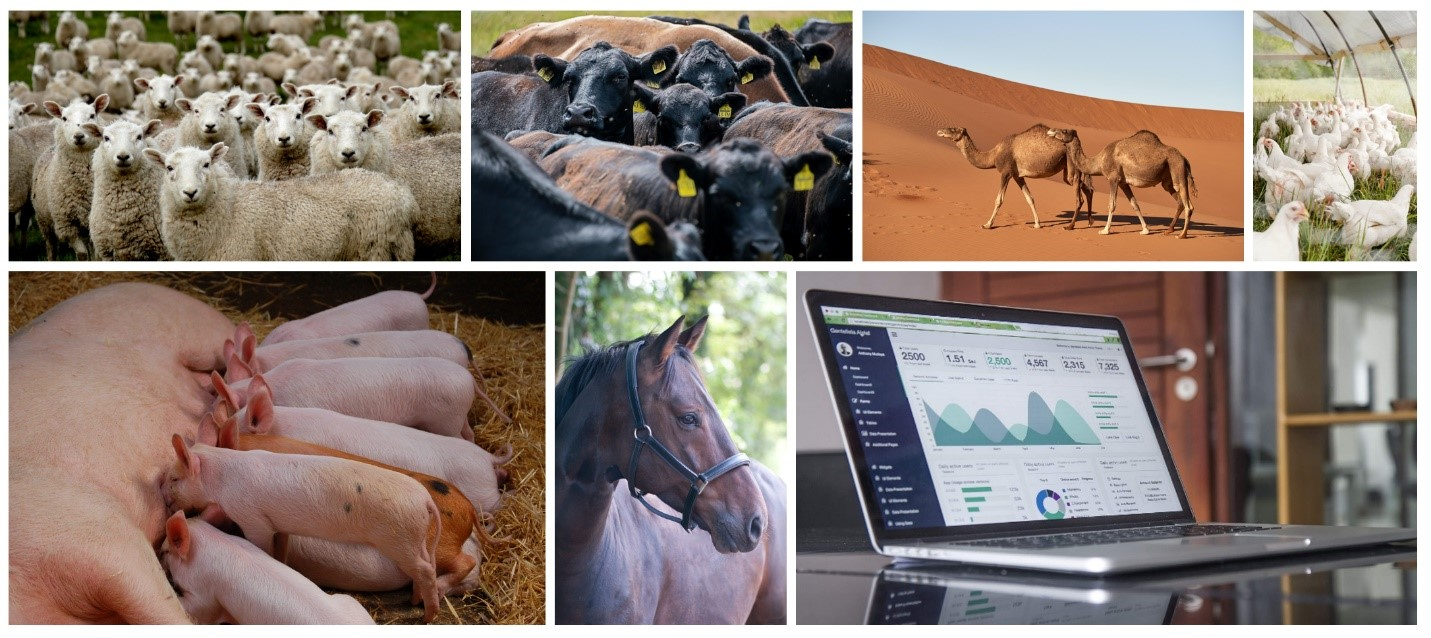
\includegraphics[keepaspectratio]{_main_files/Figures/Main_pic.jpg}}

\chapter{About this document}\label{about-this-document}

In this document you will find indications on how to use various \texttt{R} libraries and functions for estimating true disease prevalence and accuracy of diagnostic tests in a Bayesian framework, along with various exercises. We suppose that you do have some basic \texttt{R} skills. If you have not worked with \texttt{R} before or feel a bit rusty, here are some resources to help you to prepare:

\begin{itemize}
\item
  Chapters 1, 2, and 4 of the \href{https://www.codecademy.com/learn/learn-r}{CodeCademy ``Learn R'' course} will provide a good overview of the basic concepts required for this workshop.
\item
  If you are familiar with \texttt{R} and want to do some further reading, \href{https://r4ds.had.co.nz/}{Hadley Wickham's ``R for Data Science''} is a great resource.
\end{itemize}

Remember, there are often many different ways to conduct a given piece of work in \texttt{R}. Throughout this document, we tried to stick with the simpler approaches (e.g., the shortest code, the minimal number of \texttt{R} libraries).

\section{Software and libraries used}\label{software-and-libraries-used}

To conduct the exercises from this book, we will need to install three software (\texttt{R}, \texttt{RStudio}, and \texttt{JAGS}) and a few \texttt{R} packages. The installation steps are described below. These instructions are reproduced in parts from \href{https://www.r-project.org/}{R-project.org}, \href{https://posit.co/downloads/}{Rstudio.com}, and various R packages' manuals.

\subsection{R download}\label{r-download}

\texttt{R} is a language and environment for statistical computing and graphics. \texttt{R} provides a wide variety of statistical (linear and nonlinear modelling, classical statistical tests, time-series analysis, classification, clustering, \ldots) and graphical techniques, and is highly extensible.

\texttt{R} can be downloaded \href{https://cran.r-project.org/mirrors.html}{here}. You can choose in the list a CRAN mirror close to your institution; for instance, in Canada we use the mirror from \href{https://mirror.rcg.sfu.ca/mirror/CRAN/}{Simon Fraser University, Burnaby}.

\textbf{We used the 4.4.1 version of R to develop this book.}

\subsection{RStudio download}\label{rstudio-download}

\texttt{RStudio} is an integrated development environment (IDE) for \texttt{R}. It includes a console, syntax-highlighting editor that supports direct code execution, as well as tools for plotting, history, debugging and workspace management.

\texttt{RStudio} is available in open source and commercial editions and runs on the desktop (Windows, Mac, and Linux) or in a browser connected to \texttt{RStudio\ Server} or \texttt{RStudio\ Workbench}.

A free \texttt{RStudio\ Desktop\ Open\ Source\ License} can be downloaded \href{https://www.rstudio.com/products/rstudio/download/}{here}.

\textbf{We used the 2024.04.2+764 version of \texttt{RStudio} to develop this book.}

\subsection{R libraries}\label{r-libraries}

To install a given \texttt{R} library, open \texttt{RStudio}, click \texttt{Packages}, choose \texttt{load\ package}, choose the package you need (e.g., \texttt{epiR}).

For the workshop, the following \texttt{R} packages will be used:

\subsubsection{R2jags}\label{r2jags}

\textbf{Version 0.8-5} \href{/https://cran.r-project.org/web/packages/R2jags/R2jags.pdf}{R2jags manual}
The \texttt{R2JAGS} package provides convenient functions to call \texttt{rjags} (see next) and \texttt{JAGS} (a software specialized in Bayesian analyses; see below) from \texttt{R}. It automatically writes the data and scripts in a format readable by \texttt{JAGS}. After the \texttt{JAGS} process has finished, it is possible to read the resulting data into \texttt{R} using the facilities of the \texttt{coda} and \texttt{mcmcplots} packages for further analyses of the output.

\subsubsection{rjags}\label{rjags}

\textbf{Version 4-15} \href{https:/cran.r-project.org/web/packages/rjags/rjags.pdf}{rjags manual}
The \texttt{rjags} package provides an interface from \texttt{R} to the \texttt{JAGS} library for Bayesian data analysis. \texttt{JAGS} uses Markov Chain Monte Carlo (\textbf{MCMC}) to generate a sequence of dependent samples from the posterior distribution of the parameters.

\subsubsection{coda}\label{coda}

\textbf{Version 0.19-4.1} \href{https://cran.r-project.org/web/packages/coda/coda.pdf}{coda manual}\\
The \texttt{coda} package provides functions for summarizing and plotting the output from MCMC simulations, as well as diagnostic tests of convergence to the equilibrium distribution of the Markov chain.

\subsubsection{mcmcplots}\label{mcmcplots}

\textbf{Version 0.4.3} \href{https://cran.r-project.org/web/packages/mcmcplots/mcmcplots.pdf}{mcmcplots manual}\\
The \texttt{mcmcplots} package provides a function (\texttt{mcmcplot}) that produces common MCMC diagnostic plots in an html file that can be viewed from a web browser. When viewed in a web browser, hundreds of MCMC plots can be viewed efficiently by scrolling through the output as if it were any typical web page.

\subsubsection{epiR}\label{epir}

\textbf{Version 2.0.75} \href{https://cran.r-project.org/web/packages/epiR/epiR.pdf}{epiR manual}\\
The \texttt{epiR} package contains tools for the analysis of epidemiological and surveillance data. For the workshop we will mainly use \texttt{epiR} functions that can return shape parameters for different distributions, based on expert elicitation, to produce and visualize prior distributions.

\subsection{JAGS}\label{jags}

\texttt{JAGS} is a free software package for performing Bayesian inference Using Gibbs Sampling. \texttt{JAGS} stands for ``Just Another Gibbs Sampler''. It is a program for analysis of Bayesian models using MCMC simulation.

You will have to install \texttt{JAGS} on your computer for the \texttt{R2JAGS} library to work. \texttt{JAGS} can be downloaded \href{https://sourceforge.net/projects/mcmc-jags/files/}{here}.

\begin{itemize}
\tightlist
\item
  Click on the ``Download latest version JAGS-4.3.1.html'' green button;\\
\item
  Wait a few seconds;\\
\item
  Open up the JAGS-4.3.1.html file that was downloaded;\\
\item
  Pick the appropriate installation depending on the version of \texttt{R} that is installed on your computer;

  \begin{itemize}
  \tightlist
  \item
    If you have installed \texttt{R} version 4.2.0 or later, then JAGS-4.3.1 can be installed.
  \end{itemize}
\end{itemize}

\section{Some notation}\label{some-notation}

Throughout the document, you will find examples of \texttt{R} code along with comments. \textbf{The \texttt{R} code used always appear in grey boxes} (see the following example). This is the code that you will be able to use for your own analyses. \textbf{Lines that are preceded by a \# sign are comments}, they are skipped when \texttt{R} reads them. Following each grey box with \texttt{R} code, another \textbf{grey box with results from the analysis is presented}.

For instance, this is a \texttt{R} code where I am simply asking to show main descriptive statistics for the \emph{speed} variable of the \emph{cars} dataset (note that this dataset is already part of \texttt{R}).

\begin{Shaded}
\begin{Highlighting}[]
\CommentTok{\#This is a comment. R will ignore this line}

\CommentTok{\#The summary() function can be use to ask for a summary of various R objects. For a variable (here the variable speed), it shows descriptive statistics.}
\FunctionTok{summary}\NormalTok{(cars}\SpecialCharTok{$}\NormalTok{speed)}
\end{Highlighting}
\end{Shaded}

\begin{verbatim}
##    Min. 1st Qu.  Median    Mean 3rd Qu.    Max. 
##     4.0    12.0    15.0    15.4    19.0    25.0
\end{verbatim}

Throughout this document we will use:\\
- Italics for datasets or variables. For instance, the \emph{speed} variable of the dataset \emph{cars}.\\
- Shaded boxes for \texttt{R} libraries (e.g., \texttt{episensr}) and functions (e.g., \texttt{summary()}).

In \texttt{R} we can first call a given library and then use the functions related to this library or we can type the name of the library followed by \texttt{::} and then the function. For instance the two following pieces of code are equivalent:

\begin{Shaded}
\begin{Highlighting}[]
\FunctionTok{library}\NormalTok{(ggplot2)}
\FunctionTok{ggplot}\NormalTok{(}\AttributeTok{data=}\NormalTok{cars, }\AttributeTok{mapping=}\NormalTok{(}\FunctionTok{aes}\NormalTok{(}\AttributeTok{x=}\NormalTok{speed)))}\SpecialCharTok{+}
  \FunctionTok{geom\_histogram}\NormalTok{()}

\DocumentationTok{\#\#OR\#\#}

\NormalTok{ggplot2}\SpecialCharTok{::}\FunctionTok{ggplot}\NormalTok{(}\AttributeTok{data=}\NormalTok{cars, }\AttributeTok{mapping=}\NormalTok{(}\FunctionTok{aes}\NormalTok{(}\AttributeTok{x=}\NormalTok{speed)))}\SpecialCharTok{+}
  \FunctionTok{geom\_histogram}\NormalTok{()}
\end{Highlighting}
\end{Shaded}

The latter may improve reproducibility, but at the expense of longer codes. Throughout the document, we will always first call the library and then run the functions to keep codes short.

One last thing, when using a given function, it is not mandatory to name all the arguments, as long as they are presented in the sequence expected by this function. For instance, the \texttt{ggplot()} function that we used in the previous chunk of code is expecting to see first a dataset (\texttt{data=}) and then a mapping attribute (\texttt{mapping=}) and, within that mapping attribute a x variable (\texttt{x=}). We could shorten the code by omitting all of these. The two following pieces of code are, therefore, equivalent:

\begin{Shaded}
\begin{Highlighting}[]
\FunctionTok{library}\NormalTok{(ggplot2)}
\FunctionTok{ggplot}\NormalTok{(}\AttributeTok{data=}\NormalTok{cars, }\AttributeTok{mapping=}\NormalTok{(}\FunctionTok{aes}\NormalTok{(}\AttributeTok{x=}\NormalTok{speed)))}\SpecialCharTok{+}
  \FunctionTok{geom\_histogram}\NormalTok{()}

\DocumentationTok{\#\#OR\#\#  }

\FunctionTok{library}\NormalTok{(ggplot2)}
\FunctionTok{ggplot}\NormalTok{(cars, (}\FunctionTok{aes}\NormalTok{(speed)))}\SpecialCharTok{+}
  \FunctionTok{geom\_histogram}\NormalTok{()}
\end{Highlighting}
\end{Shaded}

Throughout the document, however, we will use the longer code with all the arguments being named. Since you are learning these new functions, it would be quite a challenge to use the shorter code right from the start. But you could certainly adopt the shorter codes later on.

\textbf{LET'S GET STARTED!}

\chapter{Distributions}\label{distributions}

When using latent class models (\textbf{LCM}) to estimate disease prevalence or diagnostic test accuracy, we will need to use various distributions. There are two situations where we will use distributions:

\begin{enumerate}
\def\labelenumi{\arabic{enumi})}
\tightlist
\item
  as prior distributions to describe our a priori knowledge on a given unknown parameter.\\
\item
  as a part of the likelihood function that will be used to link observed data with unknown parameters.
\end{enumerate}

Some distributions will more often be used for the first objective, others will mainly be used for the latter objective. In the following sections, we will cover the most useful distributions.

\section{Prior distributions}\label{prior-distributions}

One of the first things that we will need for any Bayesian analysis is a way to generate and visualize a prior distribution corresponding to some scientific knowledge that we have about an unknown parameter. Generally, we will use information such as the mean and variance or the mode and the 2.5th (or 97.5th) percentile to find a corresponding distribution. Here we present three of the most important distributions. We will give more details on each of them in the following sections:

\textbf{- Normal distribution:} defined by a mean (\emph{mu}) and its standard deviation (\emph{SD}) or variance (\emph{tau}). In some \texttt{R} packages and software, \texttt{rjags} and JAGS for instance, the inverse of the variance (\emph{1/tau}) is used to specify a given normal distribution.\\
\textbf{Notation: dNorm(\emph{mu}, \emph{1/tau})}

\textbf{- Uniform distribution:} defined by a minimum (\emph{min}) and maximum (\emph{max}).\\
\textbf{Notation: dUnif(\emph{min}, \emph{max})}

\textbf{- Beta distribution:} bounded between 0 and 1, beta distributions are defined by two shape parameters (\emph{a}) and (\emph{b}).\\
\textbf{Notation: dBeta(\emph{a}, \emph{b})}

\subsection{Normal distribution}\label{normal-distribution}

The \texttt{dnorm()} function can be used to generate a given Normal distribution and the \texttt{curve()} function can be used to visualize the generated distribution. These functions are already part of basic \texttt{R} functions, there is no need to upload a \texttt{R} package.

\begin{Shaded}
\begin{Highlighting}[]
\FunctionTok{curve}\NormalTok{(}\FunctionTok{dnorm}\NormalTok{(x, }
            \AttributeTok{mean=}\FloatTok{2.0}\NormalTok{, }
            \AttributeTok{sd=}\FloatTok{0.5}\NormalTok{),                                                 }\CommentTok{\# We indicate mean and SD of the distribution}
      \AttributeTok{from=}\SpecialCharTok{{-}}\DecValTok{2}\NormalTok{, }\AttributeTok{to=}\DecValTok{7}\NormalTok{,                                                 }\CommentTok{\# We indicate limits for the plot}
      \AttributeTok{main=}\StringTok{"Normal distribution with mean of 2.0 and SD of 0.5"}\NormalTok{,     }\CommentTok{\# Adding a title}
      \AttributeTok{xlab =} \StringTok{"Value"}\NormalTok{, }
      \AttributeTok{ylab =} \StringTok{"Density"}\NormalTok{)                              }\CommentTok{\# Adding titles for axes}
\end{Highlighting}
\end{Shaded}

\pandocbounded{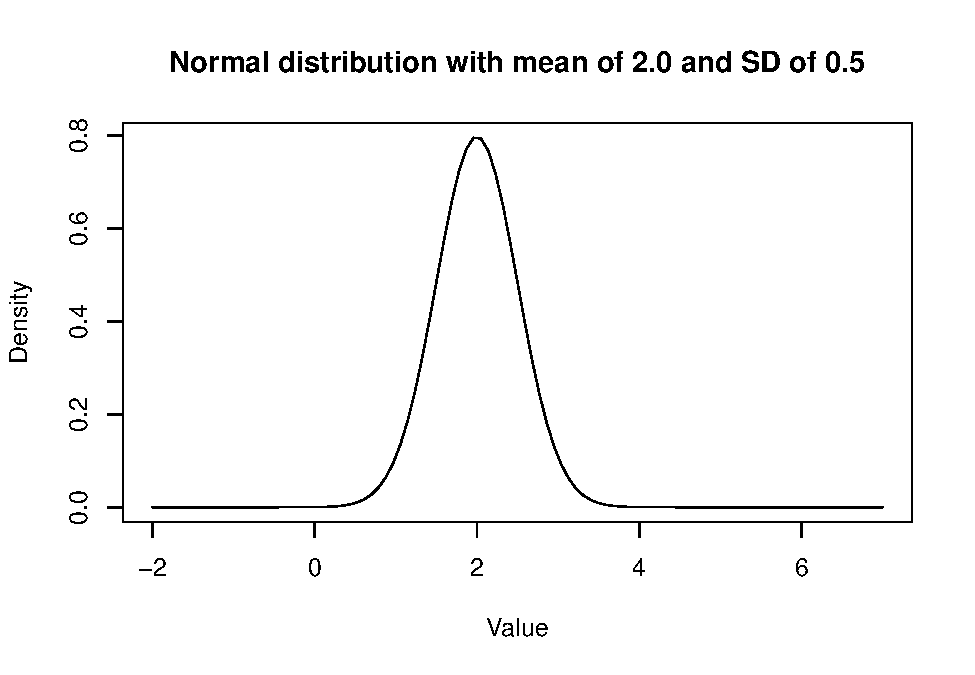
\includegraphics[keepaspectratio]{_main_files/_main_files/figure-latex/unnamed-chunk-4-1.pdf}}
Note that a Normal distribution with mean of zero and a very large \emph{SD} provides very little information. Such distribution would be referred to as \textbf{uniform or flat distribution} (A.K.A.; a vague distribution).

\begin{Shaded}
\begin{Highlighting}[]
\FunctionTok{curve}\NormalTok{(}\FunctionTok{dnorm}\NormalTok{(x, }
            \AttributeTok{mean=}\FloatTok{0.0}\NormalTok{, }
            \AttributeTok{sd=}\DecValTok{10000000000}\NormalTok{),                                    }
      \AttributeTok{from=}\SpecialCharTok{{-}}\DecValTok{100}\NormalTok{, }\AttributeTok{to=}\DecValTok{100}\NormalTok{,                                                 }
      \AttributeTok{main=}\StringTok{"A flat Normal distribution"}\NormalTok{,     }
      \AttributeTok{xlab =} \StringTok{"Value"}\NormalTok{, }
      \AttributeTok{ylab =} \StringTok{"Density"}\NormalTok{)                              }
\end{Highlighting}
\end{Shaded}

\begin{figure}
\centering
\pandocbounded{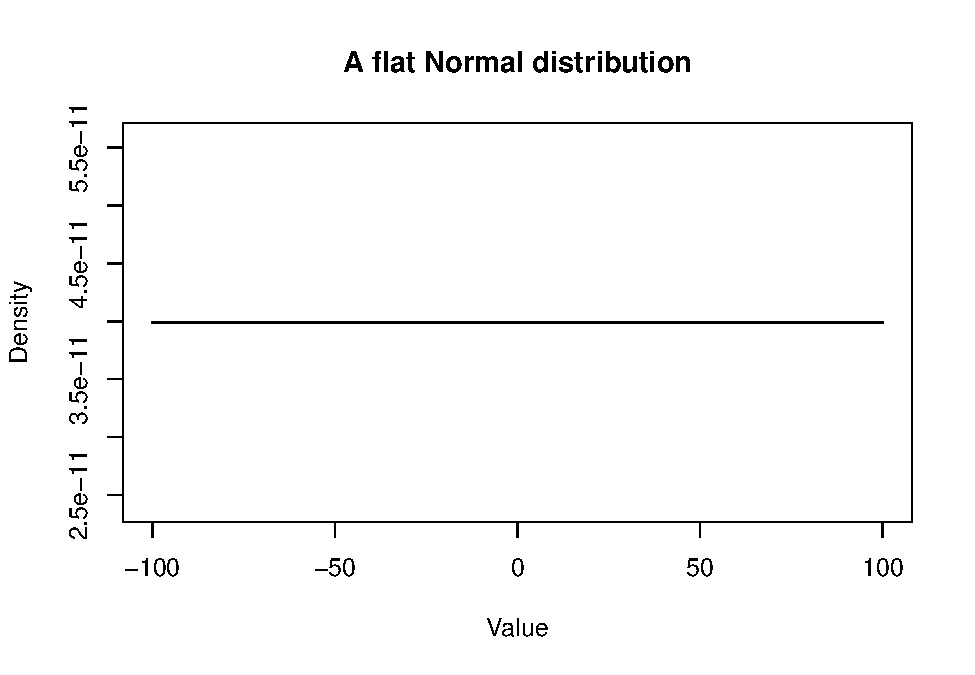
\includegraphics[keepaspectratio]{_main_files/_main_files/figure-latex/unnamed-chunk-5-1.pdf}}
\caption{\label{fig:unnamed-chunk-5}Density curve of a flat Normal distribution.}
\end{figure}

\subsection{Uniform distribution}\label{uniform-distribution}

In the same manner, we could visualize a uniform distribution using the \texttt{dunif()} function. In the following example, we assumed that any values between -5.0 and 5.0 are equally probable.

\begin{Shaded}
\begin{Highlighting}[]
\FunctionTok{curve}\NormalTok{(}\FunctionTok{dunif}\NormalTok{(x, }
            \AttributeTok{min=}\SpecialCharTok{{-}}\FloatTok{5.0}\NormalTok{, }
            \AttributeTok{max=}\FloatTok{5.0}\NormalTok{),                                    }
      \AttributeTok{from=}\SpecialCharTok{{-}}\DecValTok{10}\NormalTok{, }\AttributeTok{to=}\DecValTok{10}\NormalTok{,                                                 }
      \AttributeTok{main=}\StringTok{"Uniform distribution with {-}5.0 and 5.0 limits"}\NormalTok{,    }
      \AttributeTok{xlab =} \StringTok{"Value"}\NormalTok{, }
      \AttributeTok{ylab =} \StringTok{"Density"}\NormalTok{)                              }
\end{Highlighting}
\end{Shaded}

\begin{figure}
\centering
\pandocbounded{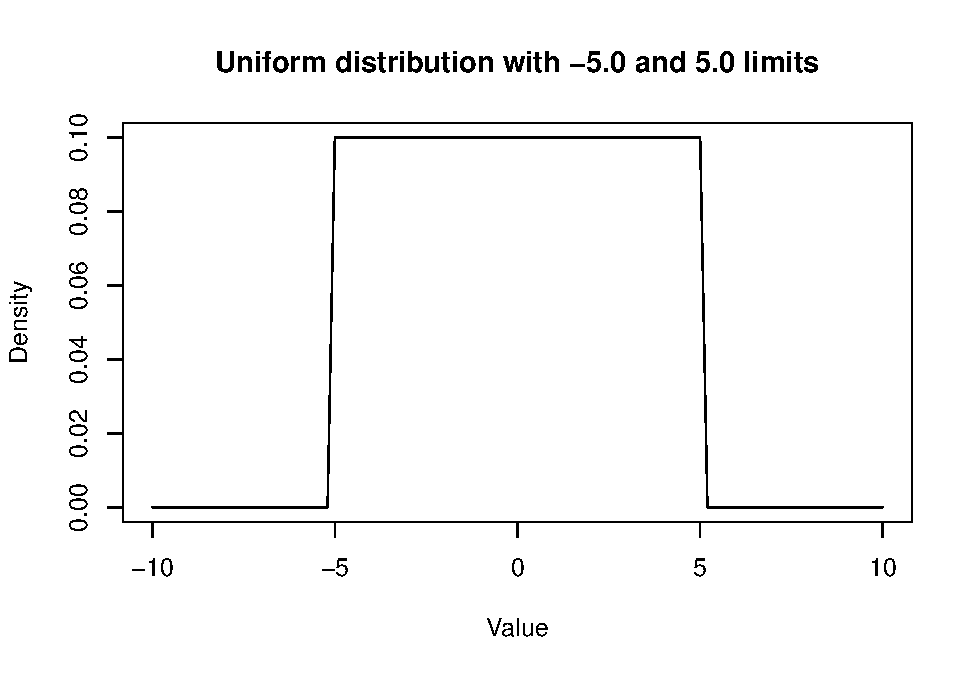
\includegraphics[keepaspectratio]{_main_files/_main_files/figure-latex/unnamed-chunk-6-1.pdf}}
\caption{\label{fig:unnamed-chunk-6}Density curve of a Uniform distribution.}
\end{figure}

\subsection{Beta distribution}\label{beta-distribution}

Beta distributions are another type of distributions that will specifically be used for parameters that are proportions (i.e., bounded between 0.0 and 1.0). For this specific workshop, they will be very handy, since sensitivity, specificity, and prevalence are all proportions. Beta distributions are defined by two shape parameters (\emph{a}) and (\emph{b}), but these parameters have no direct interpretation, as compared for instance, to the normal distribution where the first parameter is the mean and the second parameter is a measure of the variance (e.g., the standard deviation, the variance, or the inverse of the variance, depending on the software used). Nonetheless, the \emph{a} and \emph{b} parameters of a beta distribution are also related to the mean and the spread of this distribution, but as follows:

\(a = mu*psi\)\\
\(b = psi*(1-mu)\)

Where \emph{mu} is the mean of the distribution and \emph{psi} is a factor that controls the spread of the distribution. Moreover, \emph{psi} is also the sum of the \emph{a} and \emph{b} parameters of the beta distribution:

\(psi = a+b\)

From the above equations, we could also deduct that the mean of a beta distribution, \emph{mu}, can be computed as:

\(mu = a/(a+b)\)

Given that there is not direct interpretation of the \emph{a} and \emph{b} parameters of a beta distribution, it is easier to rely on a software to find the \emph{a} and \emph{b} parameters that will correspond to a desired distribution with a certain mode (or mean) and variance. The \texttt{epi.betabuster()} function from the \texttt{epiR} library can be used to define a given prior distribution based on previous knowledge. When we use the \texttt{epi.betabuster()} function, it creates a new \texttt{R} object containing different elements. Among these, one element will be named \emph{shape1} and another \emph{shape2}. These correspond to the \emph{a} and \emph{b} shape parameters of the corresponding beta distribution.

For instance, we may know that the most likely value for the sensitivity of a given test is 0.85 and that we are 97.5\% certain that it is greater than 0.75. With these values, we will be able to find the \emph{a} and \emph{b} shape parameters of the corresponding beta distribution.

Within the \texttt{epi.betabuster()} function, the \texttt{imsure=} argument will be important to indicate whether the next argument \texttt{x=0.75} describe the:\\
- 2.5th percentile (\texttt{imsure="greater\ than"}) or the\\
- 97.5th percentile (\texttt{imsure="less\ than"}).

\textbf{Typically, when the mode of a distribution is \textless50\% we suggest to use the 97.5th percentile to describe the spread of the distribution. When the mode is \textgreater50\% we suggest to use the 2.5th percentile.}

\begin{Shaded}
\begin{Highlighting}[]
\FunctionTok{library}\NormalTok{(epiR) }

\CommentTok{\# Sensitivity of a test as Mode=0.85, and we are 97.5\% sure \textgreater{}0.75 }
\NormalTok{rval }\OtherTok{\textless{}{-}} \FunctionTok{epi.betabuster}\NormalTok{(}\AttributeTok{mode=}\FloatTok{0.85}\NormalTok{,                   }\CommentTok{\# We create a new object named rval}
                       \AttributeTok{conf=}\FloatTok{0.975}\NormalTok{, }
                       \AttributeTok{imsure=}\StringTok{"greater than"}\NormalTok{, }
                       \AttributeTok{x=}\FloatTok{0.75}\NormalTok{)  }

\NormalTok{rval}\SpecialCharTok{$}\NormalTok{shape1                }\CommentTok{\#View the a shape parameter in rval}
\end{Highlighting}
\end{Shaded}

\begin{verbatim}
## [1] 62.661
\end{verbatim}

\begin{Shaded}
\begin{Highlighting}[]
\NormalTok{rval}\SpecialCharTok{$}\NormalTok{shape2                }\CommentTok{\#View the b shape parameter in rval  }
\end{Highlighting}
\end{Shaded}

\begin{verbatim}
## [1] 11.88135
\end{verbatim}

\begin{Shaded}
\begin{Highlighting}[]
\CommentTok{\#plot the prior distribution}
\FunctionTok{curve}\NormalTok{(}\FunctionTok{dbeta}\NormalTok{(x, }
            \AttributeTok{shape1=}\NormalTok{rval}\SpecialCharTok{$}\NormalTok{shape1, }
            \AttributeTok{shape2=}\NormalTok{rval}\SpecialCharTok{$}\NormalTok{shape2), }
      \AttributeTok{from=}\DecValTok{0}\NormalTok{, }\AttributeTok{to=}\DecValTok{1}\NormalTok{, }
      \AttributeTok{main=}\StringTok{"Prior for test\textquotesingle{}s sensitivity"}\NormalTok{, }
      \AttributeTok{xlab =} \StringTok{"Proportion"}\NormalTok{, }
      \AttributeTok{ylab =} \StringTok{"Density"}\NormalTok{)}
\end{Highlighting}
\end{Shaded}

\begin{figure}
\centering
\pandocbounded{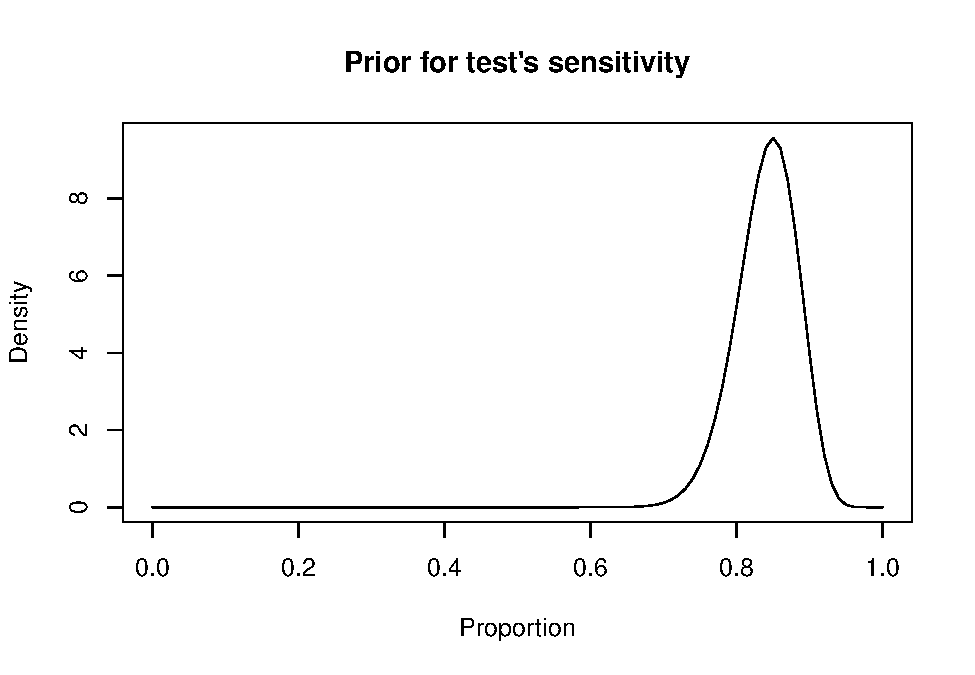
\includegraphics[keepaspectratio]{_main_files/_main_files/figure-latex/unnamed-chunk-7-1.pdf}}
\caption{\label{fig:unnamed-chunk-7}Density curve of a Beta distribution for a test sensitivity.}
\end{figure}

Note that a dBeta(1.0, 1.0) is a uniform beta distribution.

\begin{Shaded}
\begin{Highlighting}[]
\CommentTok{\#plot the prior distribution}
\FunctionTok{curve}\NormalTok{(}\FunctionTok{dbeta}\NormalTok{(x, }
            \AttributeTok{shape1=}\FloatTok{1.0}\NormalTok{, }
            \AttributeTok{shape2=}\FloatTok{1.0}\NormalTok{), }
      \AttributeTok{from=}\DecValTok{0}\NormalTok{, }\AttributeTok{to=}\DecValTok{1}\NormalTok{, }
      \AttributeTok{main=}\StringTok{"A Beta(1.0, 1.0) or flat distribution"}\NormalTok{, }
      \AttributeTok{xlab =} \StringTok{"Proportion"}\NormalTok{, }
      \AttributeTok{ylab =} \StringTok{"Density"}\NormalTok{)}
\end{Highlighting}
\end{Shaded}

\begin{figure}
\centering
\pandocbounded{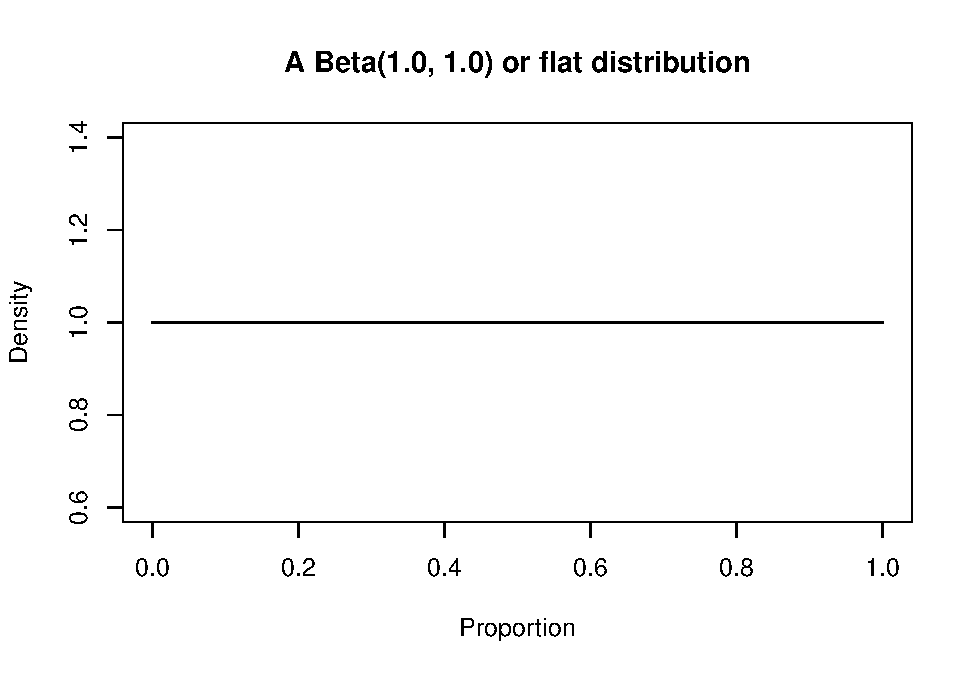
\includegraphics[keepaspectratio]{_main_files/_main_files/figure-latex/unnamed-chunk-8-1.pdf}}
\caption{\label{fig:unnamed-chunk-8}Density curve of a Beta(1.0, 1.0) distribution.}
\end{figure}

\section{Distributions for likelihood functions}\label{distributions-for-likelihood-functions}

In many situations, a distribution will be used as a part of the likelihood function to link observed data to unknown parameters. The ones we will most frequently use are:

\textbf{- Binomial distribution:} For variables that can take the value 0 or 1. Binomial distributions are defined by the probability (\emph{P}) that the variable takes the value 1 and a number of ``trials'' (\emph{n}).\\
\textbf{Notation: dBin(\emph{P}, \emph{n})}

\textbf{- Multinomial distribution:} For qualitative variables that can take more than 2 values. We can use the multinomial distribution to represent multiple probabilities, all bounded between 0 and 1, and that together will add up to 1. Multinomial distributions are defined by k probabilities (\emph{P1}, \emph{P2}, \ldots, \emph{Pk}) and the number of observations (\emph{n}).\\
\textbf{Notation: dmulti(\emph{P{[}1:k{]}}, \emph{n})}

\subsection{Binomial distribution}\label{binomial-distribution}

If we have a variable that can take only two values, healthy or diseased (0 or 1), we can estimate an unknown parameter such as the proportion (\emph{P}) of diseased individuals (i.e., the disease prevalence), based on the observed data (a number of positive individuals (\emph{T}) AND a total number of individuals (\emph{n})). For instance, if we had 30 diseased (\emph{T} = 30) out of 100 tested individuals (\emph{n} = 100) we could estimate the unknown parameter \emph{P} using this very simple likelihood function:

\(T \sim dbin(P, n)\)

\subsection{Multinomial distribution}\label{multinomial-distribution}

A last type of distribution that we will use in our LCM is the multinomial distribution. When an outcome is categorical with \textgreater2 categories, we could use a multinomial distribution to describe the probability that an individual has the value ``A'', or ``B'', or ``C'', etc. In our context, the main application of this distribution will be for describing the combined results of two (or more than two) diagnostic tests. For instance, if we cross-tabulate the results of Test A and Test B, we have four potential outcomes:

-Test A+ and Test B+ (lets call \emph{n1} the number of individuals with that combination of tests results and \emph{P1} the probability of falling in that cell)\\
-Test A+ and Test B- (\emph{n2} and \emph{P2})\\
-Test A- and Test B+ (\emph{n3} and \emph{P3})\\
-Test A- and Test B- (\emph{n4} and \emph{P4})

We can illustrate this as follow:

\begin{table}
\centering
\caption{Cross-classified results from two diagnostic tests}
\centering
\begin{tabular}[t]{l|l|l}
\hline
  & Test A+ & Test A-\\
\hline
Test B+ & n1 & n3\\
\hline
Test B- & n2 & n4\\
\hline
\end{tabular}
\end{table}

Thus we could describe the probabilities (\emph{P1} to \emph{P4}) of an individual falling into one of these cells of the 2x2 table as a multinomial distribution. In this specific case, we would say that the combined results of the 2 tests (\emph{n1} to \emph{n4}) and the total number of individual tested (\emph{n}), which are the observed data, are linked to the 4 probabilities (\emph{P1} to \emph{P4}; the unknown parameters) as follows:

\(n[1:4] \sim dmulti(P[1:4], n)\)

Which means: the value of \emph{n1} (or \emph{n2}, \emph{n3}, or \emph{n4}) is determined by the probability of falling into the ``Test A+ and Test B+'' cell, which is \emph{P1} (or \emph{P2}, \emph{P3}, or \emph{P4} for the other cells), and by the total number of individuals tested (\emph{n}). Nothing too surprising here\ldots{} If I have a probability of 0.30 to fall in a given cell, and I have tested 100 individuals, I should find 30 individuals in that cell. Wow! Still, the multinomial distribution is nice because it will ensure that all our probabilities (\emph{P1} to \emph{P4}) will sum up to exactly 1.0.

\chapter{Running Bayesian models}\label{running-bayesian-models}

Different software and \texttt{R} packages can be used to run Bayesian models. Whether it is a LCM or a more conventional regression model is not very important at this stage. In this document we will use a software called \texttt{JAGS} and the \texttt{R2jags} package. \textbf{So, if not already done, you will have to download JAGS \href{https://sourceforge.net/projects/mcmc-jags/files/}{here} and install it on your computer.}

Basically, to run any Bayesian model, we will always need the same three things:

\begin{itemize}
\tightlist
\item
  Data
\item
  A model containing:

  \begin{itemize}
  \tightlist
  \item
    A likelihood function linking observed data to unknown parameters
  \item
    A prior distribution for each unknown parameter
  \end{itemize}
\item
  An initial value for each unknown parameter to start the Markov chains

  \begin{itemize}
  \tightlist
  \item
    These values can also be generated randomly by the software, but specifying them will improve reproducibility
  \end{itemize}
\end{itemize}

\section{The data}\label{the-data}

This is the easy part. If we were to run, for instance, a ``conventional'' regression analysis, we would have to import in \texttt{R} a complete dataset (e.g., a CSV file) with a row for each observation and a column for each variable. However, when using LCM to estimate disease prevalence or diagnostic accuracy, the dataset is simply the number of individuals in each category. For instance, to estimate a simple prevalence (\emph{Prev}), we could have 30 individuals that tested positive (variable \emph{T}) out of a total of 100 individuals (variable \emph{n}). In such case, the dataset could be created as follow:

\begin{Shaded}
\begin{Highlighting}[]
\CommentTok{\#Creating a dataset}
\NormalTok{datalist }\OtherTok{\textless{}{-}} \FunctionTok{list}\NormalTok{(}\AttributeTok{T=}\DecValTok{30}\NormalTok{, }\AttributeTok{n=}\DecValTok{100}\NormalTok{)}
\end{Highlighting}
\end{Shaded}

If we want to check that it works, we could ask to see this new \texttt{R} object.

\begin{Shaded}
\begin{Highlighting}[]
\NormalTok{datalist}
\end{Highlighting}
\end{Shaded}

\begin{verbatim}
## $T
## [1] 30
## 
## $n
## [1] 100
\end{verbatim}

\section{The model}\label{the-model}

\subsection{The likelihood function}\label{the-likelihood-function}

Let's start with a simple example, estimating a single proportion. For estimating a proportion we could describe the likelihood function linking unknown parameters to observed data as follows:

\(T \sim dbin(Prev, n)\)

In other words: the disease prevalence (\emph{Prev}), an unknown parameter, can be linked to the observed number of positive individuals (\emph{T}) and the total number of tested individual (\emph{n}) through the binomial function.

In this case, the values of \emph{T} and \emph{n} are the observed data and \emph{Prev} is the only unknown parameter.

\subsection{Priors for unkown parameters}\label{priors-for-unkown-parameters}

We will have to specify a prior distribution for each unknown parameter (using the \(\sim\) sign).

In the preceding example, we only have one unkown parameter, \emph{Prev}, which is a proportion. Theoretically such parameter could take values from 0 to 1, so a beta distribution would be one way to describe its prior distribution. We could use the \texttt{epi.betabuster()} function from the \texttt{epiR} library to define a given beta distribution based on previous knowledge, as described in the previous sections. Moreover, if we want to use a flat prior, we could simply choose the value 1.0 for the a and b shape parameters.

In the following code, I am creating \texttt{R} objects for a and b for \emph{Prev} beta prior distributions.

\begin{Shaded}
\begin{Highlighting}[]
\NormalTok{Prev.shapea }\OtherTok{\textless{}{-}} \DecValTok{1}         \CommentTok{\#a shape parameter for Prev    }
\NormalTok{Prev.shapeb }\OtherTok{\textless{}{-}} \DecValTok{1}         \CommentTok{\#b shape parameter for Prev }
\end{Highlighting}
\end{Shaded}

With informative priors, for instance, if we know from the literature that the prevalence is expected to be 0.25 with 95CI of (0.20, 0.30), we could instead use the following code and assign these values to \emph{Prev.shapea} and \emph{Prev.shapeb}:

\begin{Shaded}
\begin{Highlighting}[]
\FunctionTok{library}\NormalTok{(epiR) }

\CommentTok{\# Prevalence as Mode=0.25, and we are 97.5\% sure \textless{}0.30 }
\NormalTok{rval }\OtherTok{\textless{}{-}} \FunctionTok{epi.betabuster}\NormalTok{(}\AttributeTok{mode=}\FloatTok{0.25}\NormalTok{, }
                       \AttributeTok{conf=}\FloatTok{0.975}\NormalTok{, }
                       \AttributeTok{imsure=}\StringTok{"less than"}\NormalTok{, }
                       \AttributeTok{x=}\FloatTok{0.30}\NormalTok{)  }

\NormalTok{rval}\SpecialCharTok{$}\NormalTok{shape1                }\CommentTok{\#View the a shape parameter in rval}
\end{Highlighting}
\end{Shaded}

\begin{verbatim}
## [1] 81.872
\end{verbatim}

\begin{Shaded}
\begin{Highlighting}[]
\NormalTok{rval}\SpecialCharTok{$}\NormalTok{shape2                }\CommentTok{\#View the b shape parameter in rval}
\end{Highlighting}
\end{Shaded}

\begin{verbatim}
## [1] 243.616
\end{verbatim}

\begin{Shaded}
\begin{Highlighting}[]
\CommentTok{\#The two lines below would be used to assign the generated values for later usage. Below we decided to rename this parameters Prev.shapea and Prev.shapeb since they will represent the a and b shape parameters for the Beta distribution describing the disease prevalence}
\NormalTok{Prev.shapea }\OtherTok{\textless{}{-}}\NormalTok{ rval}\SpecialCharTok{$}\NormalTok{shape1}
\NormalTok{Prev.shapeb }\OtherTok{\textless{}{-}}\NormalTok{ rval}\SpecialCharTok{$}\NormalTok{shape2}
\end{Highlighting}
\end{Shaded}

\subsection{Creating the JAGS model}\label{creating-the-jags-model}

Our Bayesian model has to be presented to JAGS as a text file (i.e., a .txt document). To create this text file, we will use the \texttt{paste0()} function to write down the model and then the \texttt{write.table()} function to save it as a .txt file.

\textbf{An interesting feature of the \texttt{paste0()} function is the possibility to include \texttt{R} objects in the text.} For instance, we may want to have a generic model that will not be modified, but within which we would like to change the values used to describe the priors. We could include these ``external'' values within our \texttt{paste0()} function. Thus, we just have to change the value of the \texttt{R} object that our model is using, rather than rewriting a new model. In the previous section, we created two \texttt{R} objects called \emph{Prev.shapea} and \emph{Prev.shapeb} (which were the a and b shape parameters for the prior distribution of our proportion \emph{Prev}). To describe our prior distribution, we can ignore this previous work that we have done and directly create a short text as follows:

\begin{Shaded}
\begin{Highlighting}[]
\NormalTok{text1 }\OtherTok{\textless{}{-}} \FunctionTok{paste0}\NormalTok{(}\StringTok{"Prev \textasciitilde{} dbeta(1, 1)"}\NormalTok{)       }\CommentTok{\#Creating a short text named "text1"}
\NormalTok{text1                                       }\CommentTok{\#Asking to see the text1 object}
\end{Highlighting}
\end{Shaded}

\begin{verbatim}
## [1] "Prev ~ dbeta(1, 1)"
\end{verbatim}

However, if the same model is to be applied later with a different prior distribution, it may be more convenient to leave the \emph{a} and \emph{b} shape parameters as \texttt{R} objects. Thus, if we change the prior distribution and run the script again, we would run the entire analyses with the newly created distribution. For instance, the code below would use the a and b shape parameters that we created above.

\begin{Shaded}
\begin{Highlighting}[]
\NormalTok{text2 }\OtherTok{\textless{}{-}} \FunctionTok{paste0}\NormalTok{(}\StringTok{"Prev \textasciitilde{} dbeta("}\NormalTok{,Prev.shapea,}\StringTok{", "}\NormalTok{,Prev.shapeb,}\StringTok{")"}\NormalTok{)            }\CommentTok{\#Creating a short text named "text2" and containing other already created R objects}
\NormalTok{text2                                                                        }\CommentTok{\#Asking to see the text2 object}
\end{Highlighting}
\end{Shaded}

\begin{verbatim}
## [1] "Prev ~ dbeta(81.872, 243.616)"
\end{verbatim}

When using \texttt{paste0()}, any text appearing outside of sets of quotation marks (e.g., \emph{Prev.shapea} and \emph{Prev.shapeb} in the preceding script) will be considered as \texttt{R} objects that need to be included in the text. Thus, later, we could just change the values for \emph{Prev.shapea} and \emph{Prev.shapeb} and our model will be automatically modified.

\textbf{Some important notes about the text file containing the model before we start with \texttt{R2jags}:}

\begin{itemize}
\item
  JAGS is expecting to see the word ``model'' followed by curly brackets \{ \}. The curly brackets will contain the likelihood function \textbf{AND} the priors.
\item
  Similarly to \texttt{R}, any line starting with a \# will be ignored (these are comments).
\item
  Similarly to \texttt{R}, \textless- means equal.
\item
  The \textasciitilde{} symbol means ``follows a distribution''.
\item
  Similarly to \texttt{R}, \texttt{JAGS} is case sensitive (i.e., \emph{P} does not equal \emph{p}).
\item
  Loops can be used with keyword ``for'' followed by curly brackets.
\item
  Array can be indicated using squared brackets {[} {]}.
\end{itemize}

In the example below, we create an \texttt{R} object called \emph{model\_single\_prop} using the \texttt{paste0()} function and then save it as a text file using the \texttt{write.table()} function. We will check this text file below and then explain the code for the model.

\begin{Shaded}
\begin{Highlighting}[]
\CommentTok{\# Specify the model}
\NormalTok{model\_single\_prop }\OtherTok{\textless{}{-}} \FunctionTok{paste0}\NormalTok{(}\StringTok{"model\{}

\StringTok{\#=== LIKELIHOOD ===\#}

\StringTok{  T \textasciitilde{} dbin(Prev, n)}


\StringTok{\#=== PRIOR  ===\#}

\StringTok{  Prev \textasciitilde{} dbeta("}\NormalTok{,Prev.shapea,}\StringTok{", "}\NormalTok{,Prev.shapeb,}\StringTok{")    \#\# Prior for Prev}

\StringTok{\}"}\NormalTok{)}

\CommentTok{\#write as a text (.txt) file}
\FunctionTok{write.table}\NormalTok{(model\_single\_prop, }
            \AttributeTok{file=}\StringTok{"model\_single\_prop.txt"}\NormalTok{, }
            \AttributeTok{quote=}\ConstantTok{FALSE}\NormalTok{, }
            \AttributeTok{sep=}\StringTok{""}\NormalTok{, }
            \AttributeTok{row.names=}\ConstantTok{FALSE}\NormalTok{,}
            \AttributeTok{col.names=}\ConstantTok{FALSE}\NormalTok{)}
\end{Highlighting}
\end{Shaded}

Here is a snapshot of the final result (i.e., the text file):

\begin{figure}
\centering
\pandocbounded{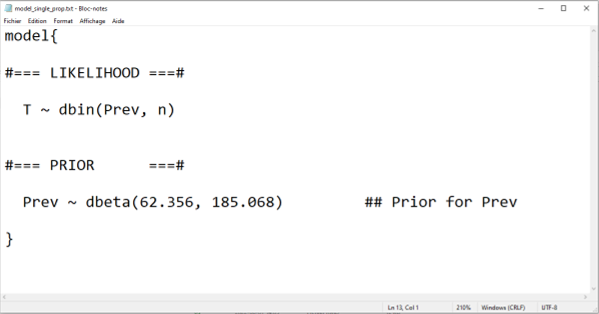
\includegraphics[keepaspectratio]{_main_files/Figures/Model_single_prop.png}}
\caption{\textbf{Text file with the model for estimating a single proportion.}}
\end{figure}

\strut \\
In the preceding script, the \texttt{paste0()} function was used to create the text, as an \texttt{R} object, that will be needed for the .txt file. This text is mainly ``static'', except for the \emph{a} and \emph{b} parameters of the beta distribution used to describe our prior knowledge on disease prevalence. We can see that, if we were to modify and then run the preceding script where we assigned values to these parameters, and then run again the \texttt{paste0()} function, our text file would be updated with new values for our prior distribution. This is a feature that we will use a lot, especially with more complex LCM, to minimize the amount of work and the risk of typographic errors..

The \texttt{write.table()} function was simply used to save, as a .txt file, the \texttt{R} object containing the text we just created.

Both the \texttt{paste0()} and \texttt{write.table()} functions are part of basic \texttt{R}, no need to install or call a given library.

\section{Generating initial values}\label{generating-initial-values}

The initial value is the first value where each Markov chain will start.\\
- We have to specify one initial value for each unknown parameter in the model.\\
- If we decide to run three Markov chains, we will need three different sets of initial values.\\
- We can also let the software choose a random value to start each chain, but it will then be impossible to \textbf{exactly} reproduce a given result. For instance, if we have obtained a very awkward Markov chain, we may not be able to reproduce this result to investigate what went wrong. Note, though, that it would be quite uncommon for a Markov chain to be extremely ``sensitive'' to the chosen starting value. But we will see during the workshop that it will sometimes happen.

In our preceding example we have one unknown parameter (\emph{Prev}). If we were to run three Markov chains, we could generate three sets of initial values for this parameter as follows. Of course, the chosen values could be changed. In the case of a proportion, we can specify any value between 0 and 1.

\begin{Shaded}
\begin{Highlighting}[]
\CommentTok{\#Initializing values for the parameter "Prev" for the 3 chains}
\NormalTok{inits }\OtherTok{\textless{}{-}} \FunctionTok{list}\NormalTok{(}
  \FunctionTok{list}\NormalTok{(}\AttributeTok{Prev=}\FloatTok{0.10}\NormalTok{),}
  \FunctionTok{list}\NormalTok{(}\AttributeTok{Prev=}\FloatTok{0.50}\NormalTok{),}
  \FunctionTok{list}\NormalTok{(}\AttributeTok{Prev=}\FloatTok{0.90}\NormalTok{)}
\NormalTok{  )}
\end{Highlighting}
\end{Shaded}

We now have an \texttt{R} object called \emph{inits} that contains the three values where each Markov chains will start.

\section{Running a model in JAGS}\label{running-a-model-in-jags}

We now have the three elements that we needed: the data, the model, and a set of initial values. We can now use the \texttt{R2jags} library to run our Bayesian analysis. The \texttt{R2jags} package provides an interface from \texttt{R} to the \texttt{JAGS} software for Bayesian data analysis. \texttt{JAGS} uses Markov Chain Monte Carlo (\textbf{MCMC}) simulation to generate a sample from the posterior distribution of the parameters.

The \texttt{R2jags} function that we will use for that purpose is the \texttt{jags()} function. Here are the arguments that we need to specify:

\begin{itemize}
\tightlist
\item
  The dataset using \texttt{data=}\\
\item
  The text file containing the model written in \texttt{JAGS} code using \texttt{model.file=}\\
\item
  The names of the parameters which should be monitored using \texttt{parameters.to.save=}\\
\item
  The number of Markov chains using \texttt{n.chains=}. The default is 3\\
\item
  The sets of initial values using \texttt{inits=}. If inits is NULL, \texttt{JAGS} will randomly generate values\\
\item
  The number of total iterations per chain (including burn-in; default: 2000) using \texttt{n.iter=}
\item
  The length of burn-in (i.e., number of iterations to discard at the beginning) using \texttt{n.burnin=}
\item
  The thinning rate, which represent how many of the values sampled by the MCMC will be retained. The default is 5 (1 out of 5). Since there is no \emph{a priori} need for thinning, we can specify \texttt{n.thin}=1 in most situations
\item
  The last argument \texttt{DIC=TRUE} or \texttt{DIC=FALSE} will determine whether to compute the deviance, pD, and deviance information criteria (\textbf{DIC}). These could sometimes be useful for model selection/comparison. We could leave that to \texttt{DIC=FALSE} since we will not be using these values during the workshop
\end{itemize}

With the following code, we will create an \texttt{R} object named \emph{bug.out}. This object will contain the results of running our model with the specified priors using the available data, and the sets of initial values that we have created. For this analysis, we have asked to run 3 Markov chains for 6000 iterations each and we discarded the first 1000 iterations of each chain. Finally, we will monitor our only unknown parameter: \emph{Prev}.

\begin{Shaded}
\begin{Highlighting}[]
\FunctionTok{library}\NormalTok{(R2jags)}
\FunctionTok{library}\NormalTok{(coda)}

\CommentTok{\#Run the Bayesian model}
\NormalTok{bug.out }\OtherTok{\textless{}{-}} \FunctionTok{jags}\NormalTok{(}\AttributeTok{data=}\NormalTok{datalist,                             }\CommentTok{\#Specifying the R object containing the data}
               \AttributeTok{model.file=}\StringTok{"model\_single\_prop.txt"}\NormalTok{,         }\CommentTok{\#Specifying the .txt file containing the model}
               \AttributeTok{parameters.to.save=}\FunctionTok{c}\NormalTok{(}\StringTok{"Prev"}\NormalTok{),               }\CommentTok{\#Specifying the parameters to monitor. When \textgreater{}1 parameter, it will be a list, ex: c("Prev", "Se", "Sp")}
               \AttributeTok{n.chains=}\DecValTok{3}\NormalTok{,                                 }\CommentTok{\#Number of chains}
               \AttributeTok{inits=}\NormalTok{inits,                                }\CommentTok{\#Specifying the R object containing the initial values  }
               \AttributeTok{n.iter=}\DecValTok{6000}\NormalTok{,                                }\CommentTok{\#Specifying the number of iterations}
               \AttributeTok{n.burnin=}\DecValTok{1000}\NormalTok{,                              }\CommentTok{\#Specifying the number of iterations to remove at the beginning}
               \AttributeTok{n.thin=}\DecValTok{1}\NormalTok{,                                   }\CommentTok{\#Specifying the thinning rate}
               \AttributeTok{DIC=}\ConstantTok{FALSE}\NormalTok{)                                  }\CommentTok{\#Indicating that we do not request the deviance, pD, nor DIC }
\end{Highlighting}
\end{Shaded}

\begin{verbatim}
## Compiling model graph
##    Resolving undeclared variables
##    Allocating nodes
## Graph information:
##    Observed stochastic nodes: 1
##    Unobserved stochastic nodes: 1
##    Total graph size: 5
## 
## Initializing model
\end{verbatim}

As we can see, we received a few messages. It looks good, don't you think?

\section{Model diagnostic}\label{model-diagnostic}

Before jumping to the results, we should first verify that:\\
- The chains have converged,\\
- The burn-in period was long enough,\\
- We have a sample of values large enough to describe the posterior distribution with sufficient precision,\\
- The Markov chains behaved well (mainly their auto-correlation).

There are many diagnostic methods available for Bayesian analyses, but, for this workshop, we will mainly use basic methods relying on plots.

Diagnostics are available when we convert our model output into a MCMC object using the \texttt{as.mcmc()} function of the \texttt{mcmcplots} library.

\begin{Shaded}
\begin{Highlighting}[]
\FunctionTok{library}\NormalTok{(mcmcplots)}
\NormalTok{bug.mcmc }\OtherTok{\textless{}{-}} \FunctionTok{as.mcmc}\NormalTok{(bug.out)          }\CommentTok{\#Converting the model output into a MCMC object (for diagnostic plots)}
\end{Highlighting}
\end{Shaded}

Then, we can apply the \texttt{mcmcplot()} function on this newly created MCMC object.

\begin{Shaded}
\begin{Highlighting}[]
\FunctionTok{mcmcplot}\NormalTok{(bug.mcmc, }\AttributeTok{title=}\StringTok{"Diagnostic plots"}\NormalTok{)        }\CommentTok{\#Asking for the diagnostic plots}
\end{Highlighting}
\end{Shaded}

When we do that, a HTML document will be created and our web browser will automatically open it. Here is a snapshot of the HTML file in our browser:

\begin{figure}
\centering
\pandocbounded{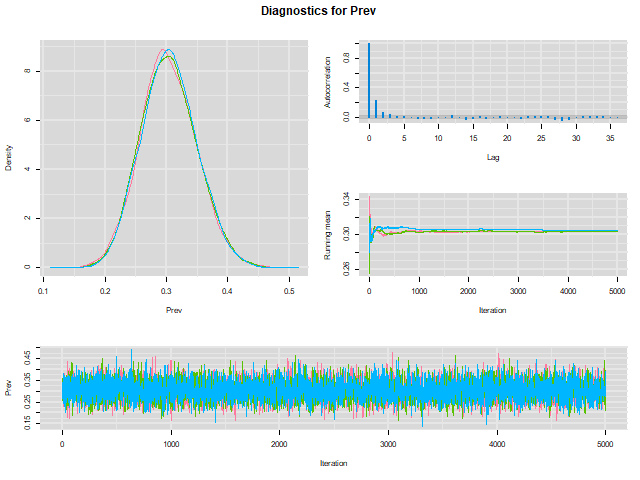
\includegraphics[keepaspectratio]{_main_files/Figures/Nice chains RM.png}}
\caption{\textbf{Diagnostic plots.}}
\end{figure}

\subsection{Convergence and burn-in}\label{convergence-and-burn-in}

To check whether convergence of the Markov chains was achieved we can inspect the ``trace plot'' (the bottom figure) presenting the values that were picked by each chain on each iteration. The different chains that we used (three in the preceding example) will be overlaid on the trace plot. We should inspect the trace plot to \textbf{evaluate whether the different chains all converged in the same area}. If so, after a number of iterations they should be moving in a relatively restricted area and this area should be the same for all chains.

The plots above would be a good example of the trace plot of three ``nice'' Markov chains (lucky us!). In this preceding example, we can see on the trace plot that the chains had already converged (probably way before the end of the first 1000 iterations that were excluded) toward the same area. On the trace plot, we can only see the values that were stored after the burn-in period. The chains were then moving freely within this limited area (thus sampling from the posterior distribution).

We could conclude based on the trace plot that:\\
- The Markov chains did converge\\
- A short burn-in period of less than a 1000 iterations would have been sufficient. Note that we will often use a longer burn-in (e.g., 5,000 or even more) just to be sure and because it only costs a few more seconds on our computer\ldots{}

Here is another example where two chains (the red and green) converged in the same area, but a third one (the blue) also converged, but in a different area. \textbf{We should be worried in such case}. We will see later the reason for such behavior.

\begin{figure}
\centering
\pandocbounded{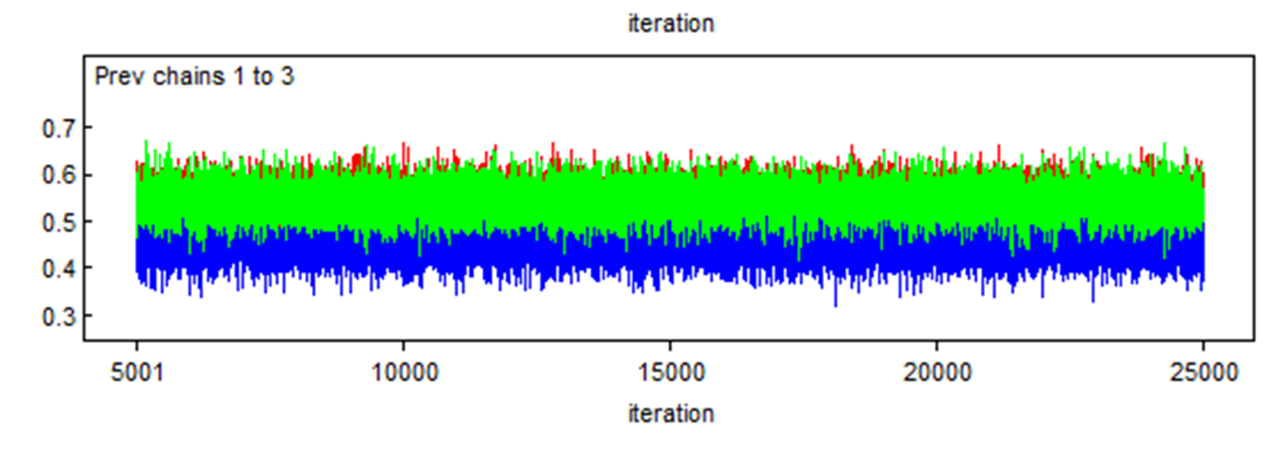
\includegraphics[keepaspectratio]{_main_files/Figures/2 nice 1 bad chain.png}}
\caption{\textbf{Trace plot - chains converging in different areas.}}
\end{figure}

\strut \\
Finally, here is a last example with just one Markov chain which clearly did not converge, even after 25,000 iterations. \textbf{We should be terrified by that!!! ;-)}.

\begin{figure}
\centering
\pandocbounded{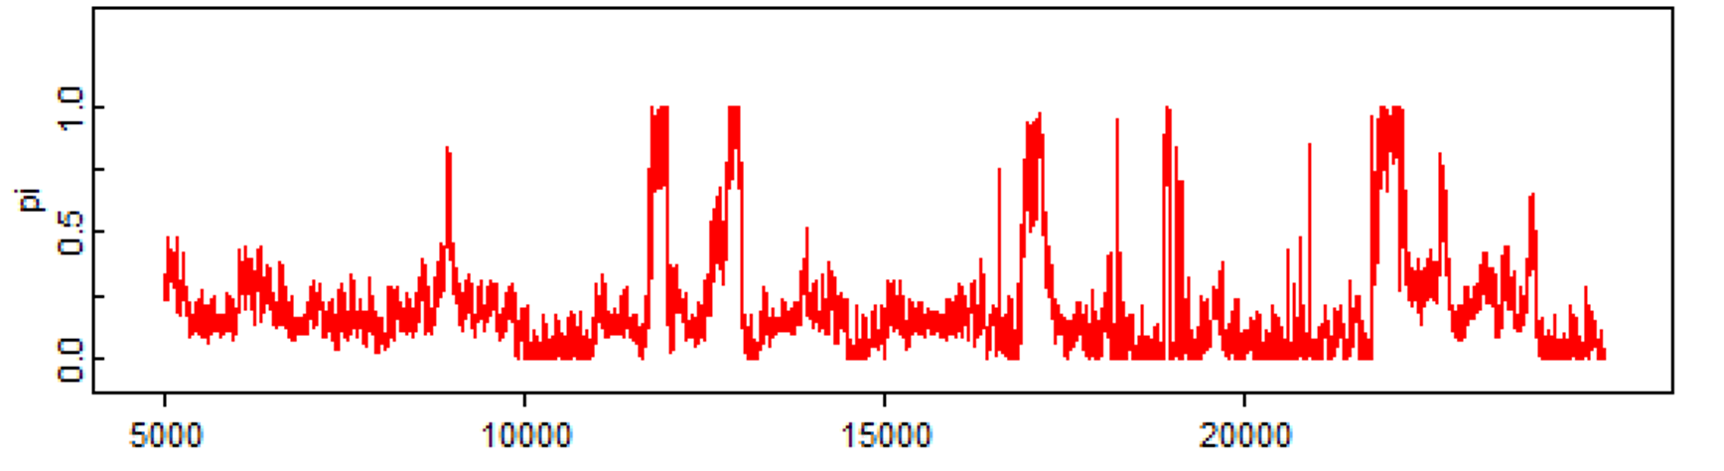
\includegraphics[keepaspectratio]{_main_files/Figures/non-conv chain.png}}
\caption{\textbf{Trace plot - a non-converging chain.}}
\end{figure}

\subsection{Number of iterations}\label{number-of-iterations}

Next, we can inspect the posterior distributions to determine if we have a large enough sample of independent values to describe with precision the median estimate and the 2.5th and 97.5th percentiles. The effective sample size (\textbf{EES}) takes into account the number of values generated by the Markov chains \textbf{AND} whether these values were auto-correlated, to compute the number of ``effective'' independent values that are used to describe the posterior distribution. Chains that are auto-correlated will generate a smaller number of ``effective values'' than chains that are not auto-correlated.

The \texttt{effectiveSize()} function of the \texttt{coda} library provide a way to appraise whether we had enough iterations. In the current example, we already created a \texttt{mcmc} object named \texttt{bug.mcmc}. We can ask for the effective sample size as follows:

\begin{Shaded}
\begin{Highlighting}[]
\FunctionTok{effectiveSize}\NormalTok{(bug.mcmc)         }\CommentTok{\#Asking for the ESS}
\end{Highlighting}
\end{Shaded}

\begin{verbatim}
##     Prev 
## 9577.497
\end{verbatim}

So we see here that, despite having stored 3 times 5,000 values (15,000 values), we have the equivalent of roughly 10,000 independent values. What to do with this information? Well, we could, for instance, decide on an arbitrary rule for ESS (say 10,000 values) and then adapt the length of the chains to achieve such an ESS \textbf{for each of the selected parameters}, because the effective sample sizes will not be the same for all parameters.

\subsection{Auto-correlation}\label{auto-correlation}

Remember that a feature of Markov chains is to have some auto-correlation between two immediately subsequent iterations, and then a correlation that quickly goes down to zero (i.e., they have a short memory). The auto-correlation plot can be used to assess if this feature is respected.

From our previous example (check the upper right figure in the plot below), it seems that it is the case.

\begin{figure}
\centering
\pandocbounded{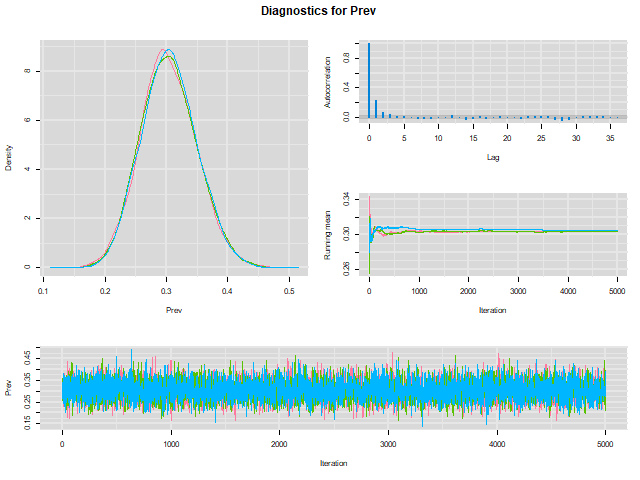
\includegraphics[keepaspectratio]{_main_files/Figures/Nice chains RM.png}}
\caption{\textbf{Autocorrelation plot with Markov chains exhibiting a short memory.}}
\end{figure}

\strut \\
Here is another example where we do have an auto-correlation that is persisting.

\begin{figure}
\centering
\pandocbounded{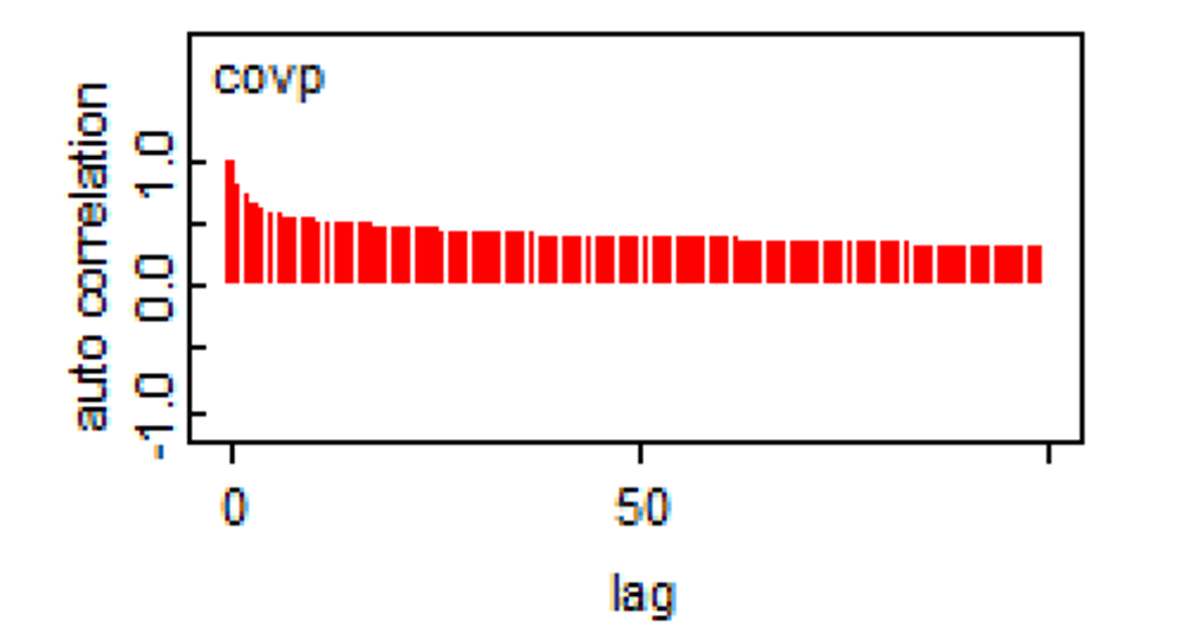
\includegraphics[keepaspectratio]{_main_files/Figures/Autocor bad.png}}
\caption{\textbf{Autocorrelation plot with Markov chains exhibiting a long memory.}}
\end{figure}

\strut \\
When such a behavior is observed, running the chains for more iterations will help achieve the desire ESS. In some situations, specifying different priors (i.e., increasing the amount of information in priors) may also help. In the past, thinning of the Markov chains (i.e., discarding all but every k\textsuperscript{th} sampled value) was often used when autocorrelation was detected, but this method is not recommended anymore, except for rare instances where computer memory limitations would be a problem \href{https://besjournals.onlinelibrary.wiley.com/doi/full/10.1111/j.2041-210X.2011.00131.x}{Link et Eaton, 2012}.

\section{Getting our estimates}\label{getting-our-estimates}

Now, if we are happy with the behavior of our Markov chains, the number of iterations, and burn-in period, we can summarize our results (i.e., report the median, 2.5th and 97.5th percentiles) very easily with the \texttt{print()} function. Below, we also indicated \texttt{digits.summary=3} to adjust the precision of the estimates that are reported (the default is 1).

\begin{Shaded}
\begin{Highlighting}[]
\FunctionTok{print}\NormalTok{(bug.out,                  }\CommentTok{\#Asking to see the mean, median, etc of the unknown parameters that were monitored}
      \AttributeTok{digits.summary=}\DecValTok{3}\NormalTok{)         }\CommentTok{\#Requiring a precision of 3 digits}
\end{Highlighting}
\end{Shaded}

\begin{verbatim}
## Inference for Bugs model at "model_single_prop.txt", fit using jags,
##  3 chains, each with 6000 iterations (first 1000 discarded)
##  n.sims = 15000 iterations saved. Running time = 0.03 secs
##      mu.vect sd.vect  2.5%   25%   50%   75% 97.5%  Rhat n.eff
## Prev   0.262   0.021 0.223 0.248 0.262 0.277 0.304 1.001 15000
## 
## For each parameter, n.eff is a crude measure of effective sample size,
## and Rhat is the potential scale reduction factor (at convergence, Rhat=1).
\end{verbatim}

Here we see that the median \emph{Prev} estimate (95BCI) was 26\% (22, 31).

We can also plot the \emph{bug.mcmc} object that we have created using the \texttt{plot()} function to produce the trace plot and a density plot presenting the posterior distributions of each unknown parameter.

\begin{Shaded}
\begin{Highlighting}[]
\FunctionTok{plot}\NormalTok{(bug.mcmc)              }\CommentTok{\#Asking for trace plot and plots of prior and posterior distributions}
\end{Highlighting}
\end{Shaded}

\begin{figure}
\centering
\pandocbounded{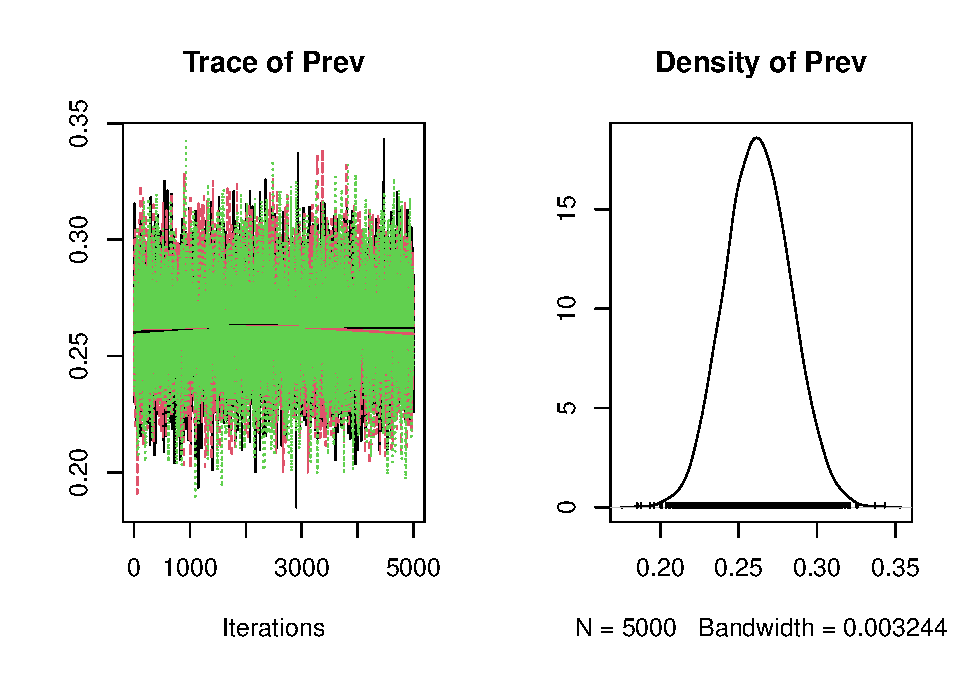
\includegraphics[keepaspectratio]{_main_files/_main_files/figure-latex/unnamed-chunk-25-1.pdf}}
\caption{\label{fig:unnamed-chunk-25}Trace plot and density plot produced using the plot() function.}
\end{figure}

If we prefer to work on our own plots, note that all the values sampled from our posterior distributions were stored in the \emph{bug.out} object that we have created. If we inspect the \emph{bug.out} object, we will notice an element named \emph{BUGSoutput}, inside this element, there is another object named \emph{sims.list}, within this \emph{sims.list}, there is an element named \emph{Prev}. As we can see below, this element is made of a list of 15,000 values. This correspond to the 5,000 values sampled (1/iteration) by each Markov chain (3 chains) for the unknown parameter \emph{Prev}. \textbf{So this element is simply all the sampled values assembled together}.

\begin{figure}
\centering
\pandocbounded{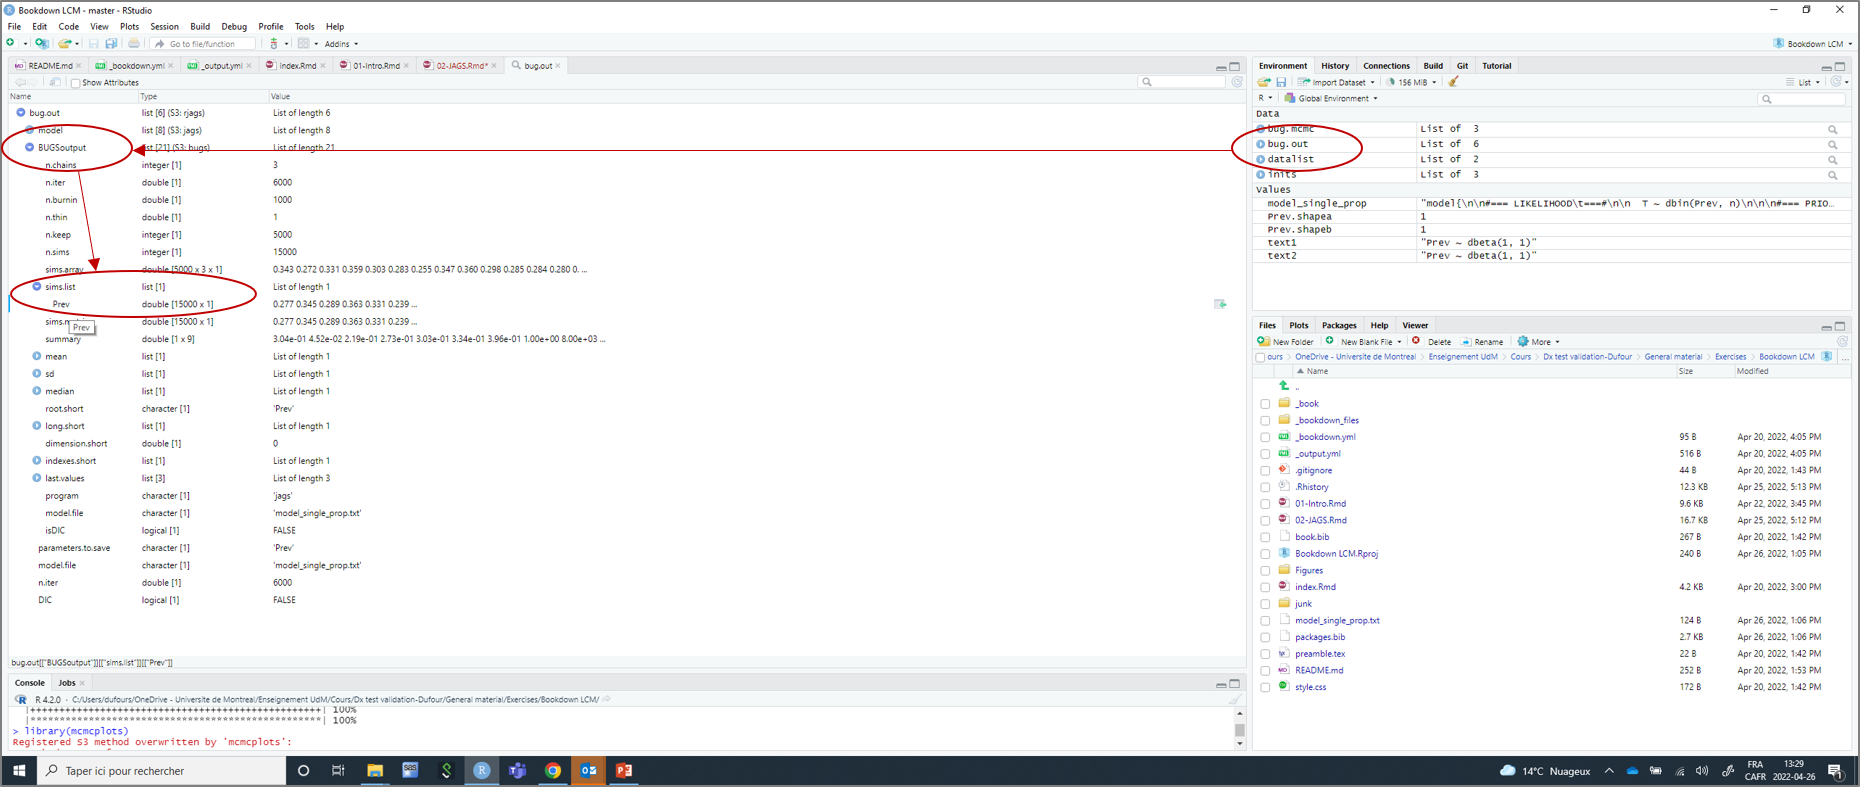
\includegraphics[keepaspectratio]{_main_files/Figures/sims list.png}}
\caption{\textbf{sims.list object located in the \emph{bug.out} output.}}
\end{figure}

\strut \\
We could use this element, for instance, to plot together the prior and posterior distributions on a same figure. On the figure below, the prior distribution is not obvious, it is the flat dashed red line just above the x axis (remember, we used a flat prior for \emph{Prev}).

\begin{Shaded}
\begin{Highlighting}[]
\CommentTok{\#Plot the posterior distribution}
\FunctionTok{plot}\NormalTok{(}\FunctionTok{density}\NormalTok{(}\AttributeTok{x=}\NormalTok{bug.out}\SpecialCharTok{$}\NormalTok{BUGSoutput}\SpecialCharTok{$}\NormalTok{sims.list}\SpecialCharTok{$}\NormalTok{Prev),      }\CommentTok{\#Indicating variable to plot}
     \AttributeTok{main=}\StringTok{"Disease prevalence"}\NormalTok{,                         }\CommentTok{\#Title for the plot}
     \AttributeTok{xlab=}\StringTok{"Prevalence"}\NormalTok{, }\AttributeTok{ylab=}\StringTok{"Density"}\NormalTok{,                 }\CommentTok{\#x and y axis titles}
\NormalTok{     )}

\CommentTok{\#plot the prior distribution}
\FunctionTok{curve}\NormalTok{(}\FunctionTok{dbeta}\NormalTok{(x, }
            \AttributeTok{shape1=}\NormalTok{Prev.shapea, }
            \AttributeTok{shape2=}\NormalTok{Prev.shapeb), }
      \AttributeTok{from=}\DecValTok{0}\NormalTok{, }\AttributeTok{to=}\DecValTok{1}\NormalTok{,          }
      \AttributeTok{lty=}\DecValTok{2}\NormalTok{,                    }\CommentTok{\#Asking for a dashed line pattern}
      \AttributeTok{col=}\StringTok{"red"}\NormalTok{,                }\CommentTok{\#Asking for a red line  }
      \AttributeTok{add=}\ConstantTok{TRUE}\NormalTok{)                }\CommentTok{\#Asking to add this plot to the preceding one}
\end{Highlighting}
\end{Shaded}

\begin{figure}
\centering
\pandocbounded{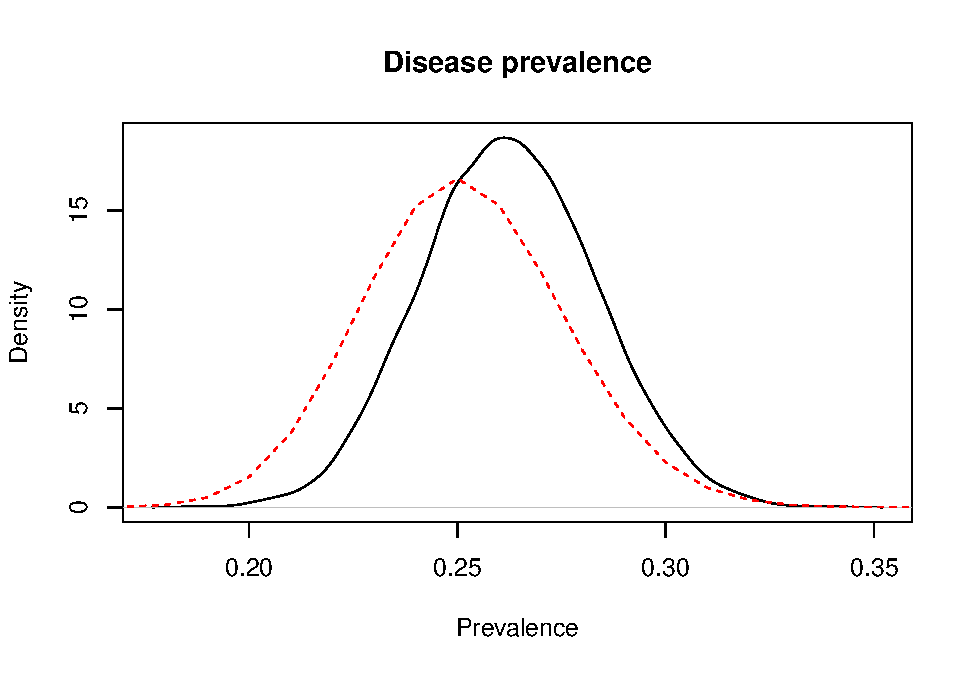
\includegraphics[keepaspectratio]{_main_files/_main_files/figure-latex/unnamed-chunk-26-1.pdf}}
\caption{\label{fig:unnamed-chunk-26}Prior (dashed red line) and posterior (full black line) distribution of the prevalence of disease.}
\end{figure}

\chapter{Exercise 1 - Proportions}\label{exercise-1---proportions}

\section{Data}\label{data}

The data used for the following exercises came from a study aiming at estimating diagnostic accuracy of a milk pregnancy associated glycoprotein (\textbf{PAG}) ELISA and transrectal ultrasonographic (\textbf{US}) exam when used for determining pregnancy status of individual dairy cows 28 to 45 days post-insemination. In that study, the new test under investigation was the PAG test and US was used for comparison, but was considered as an imperfect test.

In the original study, data from 519 cows from 18 commercial dairy herds were used. For the following exercises, the dataset was modified so that we have data from 519 cows from 3 herds (i.e., the data from 16 herds were collapsed together so they appear to be from one large herd). Note that there are some cows with missing values for one of the tests, so we will not always work with 519 cows. The complete original publication can be found here: \href{https://www.sciencedirect.com/science/article/pii/S016758771630527X?casa_token=jmHY9HiOdEYAAAAA:kGdiIujRzrAQjjFRbGqtUxIBalDGvXllp6ja9w4T2s6c7yPbgc0asnak79bJ5GWWXI8InhCg0sg}{Dufour et al., 2017}.

The dataset \emph{Preg.xlsx} contains the results from the study. However, \textbf{for the exercises we will always simply use the cross-tabulated data and these will be already organized for you and presented at the beginning of each exercise}. The dataset is still provided so you can further explore additional comparisons. The list of variables in the \emph{Preg.xlsx} dataset are described in the table below.

\textbf{Table}. List of variables in the \emph{Preg.xlsx} dataset.

\begin{longtable}[]{@{}
  >{\raggedright\arraybackslash}p{(\linewidth - 4\tabcolsep) * \real{0.1505}}
  >{\raggedright\arraybackslash}p{(\linewidth - 4\tabcolsep) * \real{0.5054}}
  >{\raggedright\arraybackslash}p{(\linewidth - 4\tabcolsep) * \real{0.3441}}@{}}
\toprule\noalign{}
\begin{minipage}[b]{\linewidth}\raggedright
\textbf{Variable}
\end{minipage} & \begin{minipage}[b]{\linewidth}\raggedright
\textbf{Description}
\end{minipage} & \begin{minipage}[b]{\linewidth}\raggedright
\textbf{Range}
\end{minipage} \\
\midrule\noalign{}
\endhead
\bottomrule\noalign{}
\endlastfoot
Obs & An observation unique ID number & 1 to 519 \\
Herd & Herd ID number & 1 to 3 \\
Cow & Cow ID number & NA \\
T1\_DOP & Number of days since insemination at testing & 28 to 45 \\
PAG\_DX & Results from the PAG test & 0 (not pregnant); 1 (pregnant) \\
US\_DX & Results from the ultrasound test & 0 (not pregnant); 1 (pregnant) \\
TRE\_DX & Results from the transrectal exam (TRE) test & 0 (not pregnant); 1 (pregnant) \\
\end{longtable}

\section{Questions}\label{questions}

We will use data from one population (herd \#1). In this herd, we had the following proportion of apparently pregnant cows (based on the US exam).

\textbf{139 US+/262 exams}

Open up the \texttt{R} project for Exercise 1 (i.e., the R project file named \emph{Exercise 1.Rproj}).

In the Exercise 1 folder, you will find partially completed \texttt{R} scripts. To answer the questions, try to complete the missing parts (they are highlighted by a \textbf{\#TO COMPLETE\#} comment). We also provided complete \texttt{R} scripts, but try to work it out on your own first!

\textbf{1. Start from the partially completed \emph{Question 1.R} script located in Exercise 1 folder.} What would be the proportion of pregnant cows? Use a Bayesian approach to compute that proportion and a credible interval (\textbf{CI}). For this first computation, assume that we have no prior knowledge on the expected proportion of pregnant cows in a Canadian herd. Run three Markov chains with different sets of initial values. Look at the trace plot. Do you think convergence was achieved? Do you need a longer burn-in period? Are all 3 chains converging in the same space? Compute the effective sample size (\textbf{ESS}), do you feel that number of iterations was sufficient to describe the posterior distribution with enough precision? What about auto-correlation of the Markov chains, any issues there?

\textbf{2.} If we were to compute a Frequentist estimate with 95\% CI, would it differ a lot from our Bayesian estimates? Why? As a refresher, the formula for a Frequentist 95\%CI for a proportion is below (where \emph{P} is the actual observed proportion and \emph{n} is the denominator for that proportion):

\(95CI=P \pm 1.96* \sqrt{\frac{P*(1-P)}{n}}\)

\textbf{3. Start from the partially completed \emph{Question 3.R} script located in Exercise 1 folder.} We just found that \href{https://www.sciencedirect.com/science/article/pii/S0093691X06001543?via\%3Dihub}{Romano et al.~(2006)} reported, for a US exam conducted between 28-45 days post-insemination:\\
-Sensitivity (\textbf{Se}) = 0.90 (95CI: 0.85, 0.95)\\
-Specificity (\textbf{Sp}) = 0.95 (95CI: 0.90, 0.97)

We now realized that, since a US exam is not a gold-standard test, in the previous exercises we rather computed an apparent prevalence (\textbf{AP}), not the true prevalence (\textbf{P}). From the literature, we know that these two parameters are linked as follow:

\(AP= Se*P + (1-Sp)*(1-P)\)

Knowing that we had the following proportion of apparently pregnant cows (based on the US exam).

\textbf{139 US+/262 exams}

And assuming, again, that we have no prior knowledge on the expected proportion of pregnant cows in a Canadian herd.

Can you think of a way to estimate the true prevalence, rather than the apparent prevalence, using that formulae?

\textbf{4. Start from the \texttt{R} script that you completed in Question 1.} In the literature, we saw a recent study conducted on 30 Canadian herds and reporting an expected pregnancy prevalence of 42\% with 97.5\% percentile of 74\%. What kind of distribution could we use to represent this information? Use these information as a pregnancy prevalence prior distribution to compute an apparent prevalence. Are your results very different from those of Question 1?

\textbf{5. Start from the partially completed \emph{Question 5.R} script located in Exercise 1 folder.} When comparing PAG to US results in herd \#1, we got the following 2x2 table.

\textbf{Table.} Cross-classified results of the PAG and US tests in herd \#1.

\begin{longtable}[]{@{}cccc@{}}
\toprule\noalign{}
& \textbf{US+} & \textbf{US-} & \textbf{Total} \\
\midrule\noalign{}
\endhead
\bottomrule\noalign{}
\endlastfoot
\textbf{PAG+} & 138 & 10 & 148 \\
\textbf{PAG-} & 1 & 113 & 114 \\
\textbf{Total} & 139 & 123 & 262 \\
\end{longtable}

\textbf{Assuming that US is a gold-standard test} could we compute PAG sensitivity (\textbf{Se}) and specificity (\textbf{Sp})? Use vague priors for PAG \emph{Se} and \emph{Sp} since it is the first ever study on this topic (i.e., we do not have any prior knowledge on these unknown parameters).

\section{Answers}\label{answers}

\textbf{1.} What would be the proportion of pregnant cows? Use a Bayesian approach to compute that proportion and a Bayesian credible interval (\textbf{BCI}). For this first computation, assume that we have no prior knowledge on the expected proportion of pregnant cows in a Canadian herd. Run three Markov chains with different sets of initial values. Look at the trace plot. Do you think convergence was achieved? Do you need a longer burn-in period? Are all 3 chains converging in the same space? Compute the effective sample size (\textbf{ESS}), do you feel that number of iterations was sufficient to describe the posterior distribution with enough precision? What about auto-correlation of the Markov chains, any issues there?

\textbf{Answer:} I chose to run a model with 3 chains of 10,000 iterations each (11,000 iterations minus a burn-in of 1,000). I have obtained the following diagnostic plots:

\begin{figure}
\centering
\pandocbounded{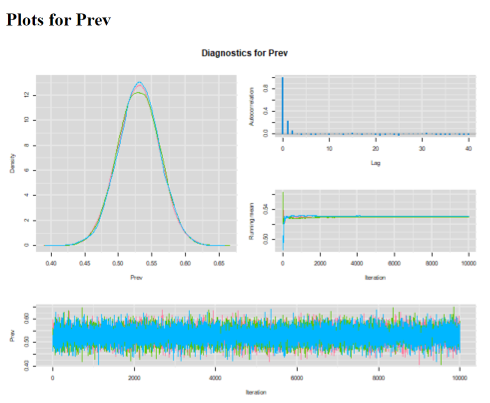
\includegraphics[keepaspectratio]{_main_files/Figures/Ex1_Q1_Dx.png}}
\caption{\textbf{Diagnostic plot}}
\end{figure}

\strut \\
Convergence of the 3 chains was achieved, all three chains appear to be moving in the same space (see trace plot). The 1,000 iterations burn-in period is probably more than needed for this very simple problem. Autocorrelation plot is just perfect with correlation declining very rapidly close to zero at lag of 1! The effective sample size for the \emph{Prev} parameter is \textgreater18,000 values. So, plenty of precision to report the median and 2.5th and 97.5th percentiles.

The median pregnancy prevalence estimate (95\% CI) was 53.0\% (46.9, 59.0).

\textbf{2.} If we were to compute a Frequentist estimate with 95\% CI, would it differ a lot from our Bayesian estimates? Why?

\textbf{Answer:} It should not differ much from the Bayesian median estimate and 95CI because these latter estimates were generated using vague priors. In such cases, Bayesian and Frequentist estimates should be quite similar. Actually, if we use the Frequentist formula for computing 95CI and the observed data (i.e., 139/262) we get:

\(P = 139/262 = 0.531\)

\(95CI=0.531 \pm 1.96* \sqrt{\frac{0.531*(1-0.531)}{262}} = 0.531 \pm 0.060\)

Thus, we have a Frequentist estimated proportion of 53.1\% with a Frequentist 95 CI of 47.1 to 59.1 (virtually unchanged compared to the Bayesian estimates).

\textbf{3.} Can we think of a way to estimate the true prevalence, rather than the apparent prevalence, using that formulae?

\textbf{Answer:} That was a tricky question don't we think? Below is the model we used for that:

\begin{figure}
\centering
\pandocbounded{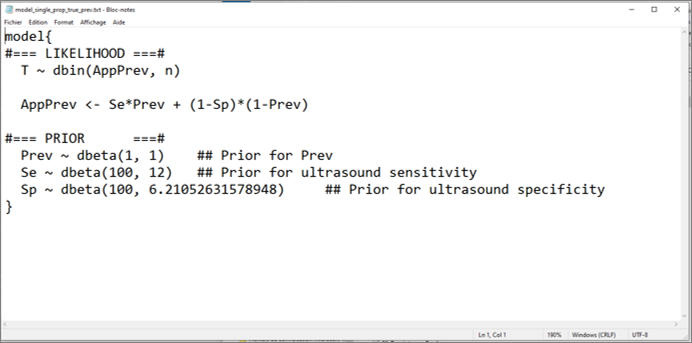
\includegraphics[keepaspectratio]{_main_files/Figures/model_single_prop_true_prev.png}}
\caption{\textbf{Model used to estimate true prevalence}}
\end{figure}

\strut \\
It may a bit disturbing at first sight, but we did not try to isolate the true prevalence (\emph{Prev}) to the left side of the equation relating the apparent (\emph{AppPrev}) and true prevalence (\emph{Prev}). This is because Bayesian models are not necessarily read from left to right, but rather as a big ``spaghetti bowl''. In short, there is no need for a left to right form of mathematical writing. As long as we explain how the two parameters \emph{AppPrev} and \emph{Prev} are linked, the model will make sense of this.

Then, you may also have noticed that we provided prior distributions for \emph{Prev}, an unknown parameter, and also for US sensitivity and specificity (\emph{Se} and \emph{Sp}). But we did not specify any prior distribution for the apparent prevalence (\emph{AppPrev}). Indeed, \emph{AppPrev} is also an unknown parameter, but it was directly defined by the equation linking the true (\emph{Prev}) and apparent prevalence (\emph{AppPrev}). Therefore, there is no need for specifying a prior distribution for \emph{AppPrev}.

Using this model, we were able to estimate that the \textbf{median (95\% BCI) true prevalence was 56.7\% (48.4, 65.4)}. As a comparison, the \textbf{median (95\% BCI) apparent prevalence was estimated at 53.1\% (47.1, 59.1)}. You may have noted that the width of the 95\% BCI for the true prevalence (17.0 percentage-points) is larger than that of the apparent prevalence (12 percentage-points). It is because we combined the uncertainty regarding the prevalence with the uncertainty regarding ultrasound sensitivity and specificity, when computing the true prevalence. For computing the apparent prevalence, we only considered the uncertainty regarding this latter proportion.

\textbf{4.} In the literature, we saw a recent study conducted on 30 Canadian herds and reporting an expected pregnancy prevalence of 42\% with 97.5\% percentile of 74\%. What kind of distribution could we use to represent this information? Use these information as a pregnancy prevalence prior distribution to compute an apparent prevalence. Are our results very different from those of Question 1?

\textbf{Answer:} A beta(4.2, 5.4) distribution would have a mode of 0.42 and a 97.5th percentile of 0.74. Using this information as prior, I get a prevalence of pregnancy of 52.7\% (95 CI: 46.8, 58.6). Actually, we observe very little difference between the models using vague \emph{vs.} informative priors. This is because this informative prior contains only the equivalent of 10 observations \((4.2+5.4)\). In the dataset, there are 262 cows. Therefore, the estimation process is still mainly driven by our dataset.

\textbf{5.} Assuming that US is a gold-standard test could you compute PAG sensitivity (\textbf{Se}) and specificity (\textbf{Sp})? Use vague priors for PAG \emph{Se} and \emph{Sp} since it is the first ever study on this topic (i.e., we do not have any prior knowledge on these unknown parameters).

\textbf{Answer:} The sensitivity and specificity are simple proportions. Sensitivity is simply the number of test positive among the number of truly diseased individuals. We have data for these in the 2x2 table. If we assume that \emph{US} is a gold-standard test, then the number of truly diseased cows is 139. Of them, 138 tested positive to the \emph{PAG} test. Similarly, the specificity is simply the number of test negative among the number of truly healthy individuals. From the 2x2 table, the number of true negative cows was 123 and 113 of them tested negative to the \emph{PAG} test. The likelihood functions (one for each parameter in this case) linking the unknown parameters (\emph{Se} and \emph{Sp}) to these observed data would be:

\(Test+ \sim dbin(Se, True+)\)

\(Test- \sim dbin(Sp, True-)\)

Using vague beta(1, 1) priors on the \emph{Se} and \emph{Sp}, I got an estimated \emph{Se} of 98.8\% (95 CI: 96.1, 99.8) and a \emph{Sp} of 91.5\% (95CI: 85.9, 95.5). \textbf{But be cautious with these numbers.} We know very well that an \emph{US} exam is not a perfect diagnostic test for pregnancy in dairy cows. With the current approach, we are attributing all disagreements between tests to a failure of the \emph{PAG} test\ldots{} But it could be the \emph{US} test that was wrong in many instances. Moreover, animals for which the two tests agreed could still be misdiagnosed as pregnant or open, but by both tests (i.e., a failure of the \emph{PAG} \textbf{AND} the \emph{US} tests). We wil see in the next sections of the course how to account for the fact that neither of the tests are gold-standards.

\chapter{Two imperfect tests}\label{two-imperfect-tests}

When using two imperfect diagnostic tests on the same population, we will have to use a Bayesian latent class model (\textbf{LCM}) to estimate the true disease prevalence, and the sensitivity and specificity of both diagnostic tests. Two different approaches could be used. The simplest approach would be to consider that the two diagnostic tests are independent conditionally on the true health status of the individuals. Conditional independence can be defined as:

\emph{Two tests are conditionally independent when the sensitivity (or specificity) of one test does not depend on whether the results of another test are positive or negative among infected (or non-infected) individuals.} \href{https://doi.org/10.20506/rst.40.1.3224}{Cheung et al., 2021}

In many situations, however, we will use two diagnostic tests that make use of the same biological process. For instance, an ELISA test could measure antibodies against a given pathogen in blood and another test could also measure antibodies, but in milk. In such case, it would be difficult to pretend that:

\emph{The sensitivity of the milk test does not depend on whether the results of the blood test are positive or negative among infected individuals.}

Therefore, it would be better to consider a LCM where conditional dependence between tests is possible. Note that, even for tests that make use of very different biological processes, it is rather difficult (or, actually, often impossible) to ``demonstrate'' conditional independence between them. So, if doable, allowing for a potential conditional dependence between tests would be a more robust strategy.

\section{Assuming conditional independence}\label{assuming-conditional-independence}

When two tests are conditionally independent, then obtaining a given combination of results to Test A and Test B, as function of the true disease prevalence (\emph{P}) and of the accuracy of each test (\emph{SeA}, \emph{SpA}, \emph{SeB}, \emph{SpB}) can be described as illustrated below:

\begin{figure}
\centering
\pandocbounded{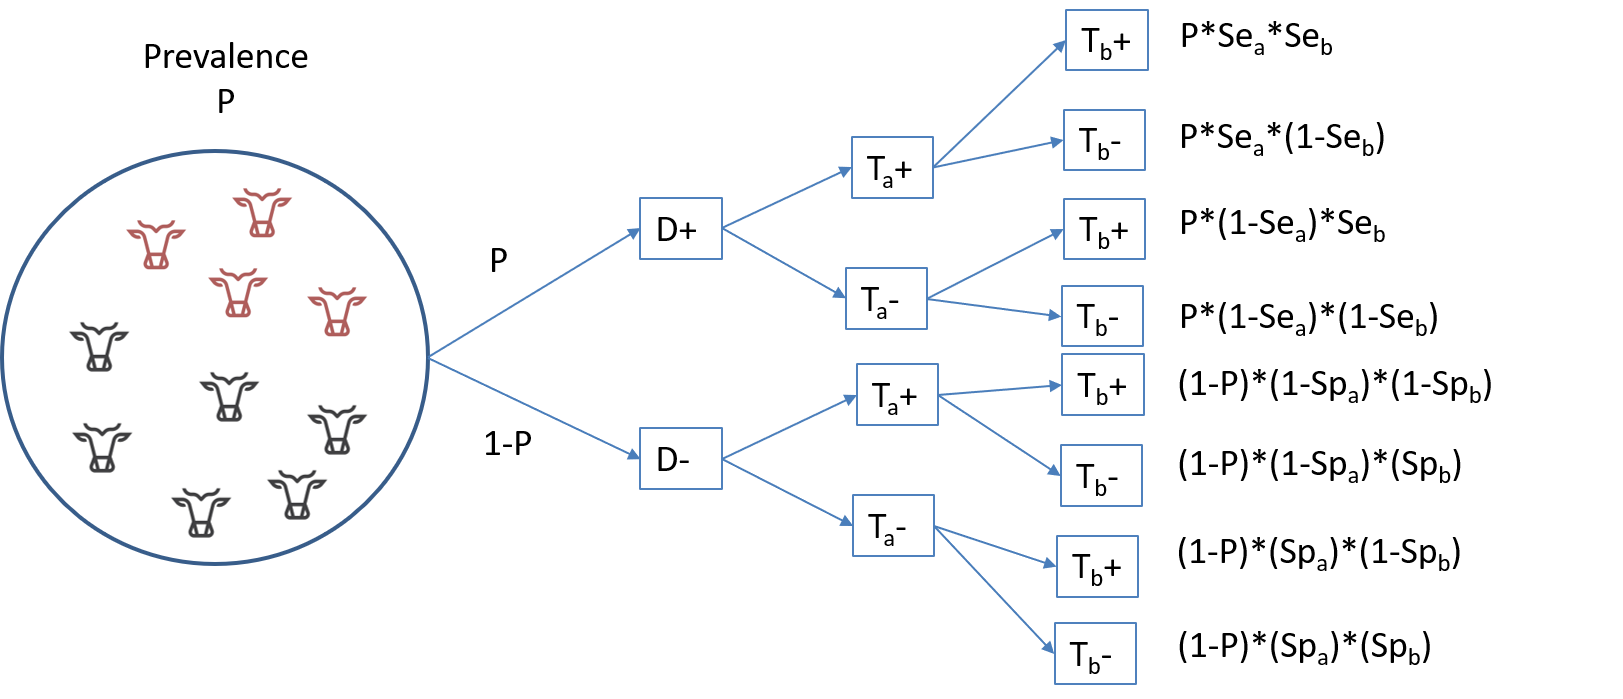
\includegraphics[keepaspectratio]{_main_files/Figures/cond_indep.png}}
\caption{\textbf{Illustration of the different potential results when applying two conditionally independent tests in a population.}}
\end{figure}

\strut \\
From that illustration, we can deduce that the probability of testing positive to both tests is the sum of the first and fifth rows:

\(P(TestA+ TestB+) = P*SeA*SeB + (1-P)*(1-SpA)*(1-SpB)\)

Or, putted in words, it is the probability of being a truly diseased individual and of being identified as such by both tests (\(P*SeA*SeB\)), plus the probability of being a healthy individual and being misdiagnosed as diseased by both tests (\((1-P)*(1-SpA)*(1-SpB)\)). If we extend this reasoning to all tests combination possibilities, we get:

\(P(TestA+TestB+) = P*SeA*SeB + (1-P)*(1-SpA)*(1-SpB)\)\\
\(P(TestA+TestB-) = P*SeA*(1-SeB) + (1-P)*(1-SpA)*SpB\)\\
\(P(TestA-TestB+) = P*(1-SeA)*SeB + (1-P)*SpA*(1-SpB)\)\\
\(P(TestA-TestB-) = P*(1-SeA)*(1-SeB) + (1-P)*SpA*SpB\)

When applying two diagnostic tests on a given population, the data generated can be presented very simply as the number of individuals in each cell of the 2x2 table presenting the cross-classified results of the two tests:

\begin{table}
\centering
\caption{Cross-classified results from two diagnostic tests}
\centering
\begin{tabular}[t]{l|l|l}
\hline
  & Test A+ & Test A-\\
\hline
Test B+ & n1 & n3\\
\hline
Test B- & n2 & n4\\
\hline
\end{tabular}
\end{table}

Thus, the likelihood function that could link the observed data (\emph{n1}, \emph{n2}, \emph{n3}, \emph{n4}) to the unknown parameters (\emph{P}, \emph{SeA}, \emph{SeB}, \emph{SpA}, \emph{SpB}) could be defined as follows, using a multinomial distribution:

\(n[1:4] \sim dmulti(P[1:4], n)\)

\(P1 = P*SeA*SeB + (1-P)*(1-SpA)*(1-SpB)\)\\
\(P2 = P*SeA*(1-SeB) + (1-P)*(1-SpA)*SpB\)\\
\(P3 = P*(1-SeA)*SeB + (1-P)*SpA*(1-SpB)\)\\
\(P4 = P*(1-SeA)*(1-SeB) + (1-P)*SpA*SpB\)

Again, if we put that in words, the number of individuals in cell \emph{n1} (i.e., TestA+ and TestB+) is determined by the number of individuals tested (\emph{n}) and the probability (\emph{P1}) of falling in that cell. The latter itself depends on the true prevalence of disease in the population (\emph{P}), and on each of the two tests sensitivity (\emph{SeA} and \emph{SeB}) and specificity (\emph{SpA} and \emph{SpB}). We can use similar reasoning for \emph{n2}, \emph{n3}, and \emph{n4}. Finally, the multinomial distribution would further impose that the four probabilities (\emph{P1}, \emph{P2}, \emph{P3}, and \emph{P4}) have to sum up to 1.0 (i.e., 100\%).

In such a model, we will have five unknown parameters to estimate (\emph{P}, \emph{SeA}, \emph{SeB}, \emph{SpA}, \emph{SpB}), but only four equations. Thus, the model will be ``non-identifiable'', and we will need to provide informative priors on, at least, two parameters. Often, we will provide priors on the Se and Sp of one of the tests, and/or on disease prevalence.

To run such a model, we simply need to provide a dataset where \emph{n1}, \emph{n2}, \emph{n3}, and \emph{n4} are listed (in that order).

\begin{Shaded}
\begin{Highlighting}[]
\CommentTok{\#n is of the form : (TestA pos and TestB pos), (TestA pos and TestB neg), (TestA neg and TestB pos), then (TestA neg and TestB neg)}
\NormalTok{datalist }\OtherTok{\textless{}{-}} \FunctionTok{list}\NormalTok{(}\AttributeTok{n=}\FunctionTok{c}\NormalTok{(}\DecValTok{138}\NormalTok{,}\DecValTok{1}\NormalTok{,}\DecValTok{10}\NormalTok{,}\DecValTok{113}\NormalTok{))}
\end{Highlighting}
\end{Shaded}

Moreover, we will need the following information to generate the \emph{a} and \emph{b} shape parameters of the various distributions. These values will be included in the text file presenting the \texttt{JAGS} model. Note that we used below the \texttt{paste0()} function to produce a model in which we could modify the tests ``labels''. We could thus use the \texttt{JAGS} model that will be described next as a generic model for various diagnostic tests, and still obtain ``meaningful'' outputs.

\begin{Shaded}
\begin{Highlighting}[]
\CommentTok{\#We could first create labels for TestA and TestB}
\NormalTok{TestA }\OtherTok{\textless{}{-}} \StringTok{"US"}
\NormalTok{TestB }\OtherTok{\textless{}{-}} \StringTok{"PAG"}

\CommentTok{\#Provide information for the prior distributions (all beta distributions) for the 5 unknown parameters }
\CommentTok{\#Below, we have used informative priors for Prev, and Se and Sp of Test A. The values used are not seldom important at this stage.}
\NormalTok{Prev.shapea }\OtherTok{\textless{}{-}} \FloatTok{4.2}         \CommentTok{\#a shape parameter for Prev    }
\NormalTok{Prev.shapeb }\OtherTok{\textless{}{-}} \FloatTok{5.4}         \CommentTok{\#b shape parameter for Prev}

\NormalTok{Se.TestA.shapea }\OtherTok{\textless{}{-}} \DecValTok{131}     \CommentTok{\#a shape parameter for Se of TestA}
\NormalTok{Se.TestA.shapeb }\OtherTok{\textless{}{-}} \DecValTok{15}      \CommentTok{\#b shape parameter for Se of TestA}
\NormalTok{Sp.TestA.shapea }\OtherTok{\textless{}{-}} \DecValTok{100}     \CommentTok{\#a shape parameter for Sp of TestA}
\NormalTok{Sp.TestA.shapeb }\OtherTok{\textless{}{-}} \DecValTok{6}       \CommentTok{\#b shape parameter for Sp of TestA}

\NormalTok{Se.TestB.shapea }\OtherTok{\textless{}{-}} \DecValTok{1}       \CommentTok{\#a shape parameter for Se of TestB}
\NormalTok{Se.TestB.shapeb }\OtherTok{\textless{}{-}} \DecValTok{1}       \CommentTok{\#b shape parameter for Se of TestB}
\NormalTok{Sp.TestB.shapea }\OtherTok{\textless{}{-}} \DecValTok{1}       \CommentTok{\#a shape parameter for Sp of TestB}
\NormalTok{Sp.TestB.shapeb }\OtherTok{\textless{}{-}} \DecValTok{1}       \CommentTok{\#b shape parameter for Sp of TestB}

\CommentTok{\#We will also need the total number of individuals tested (n)}
\NormalTok{n }\OtherTok{\textless{}{-}} \FunctionTok{sapply}\NormalTok{(datalist, sum)}
\end{Highlighting}
\end{Shaded}

With that, we have everything that is needed to write the \texttt{JAGS} model.

\begin{Shaded}
\begin{Highlighting}[]
\CommentTok{\#Create the JAGS text file}
\NormalTok{model\_2tests\_1pop\_indep }\OtherTok{\textless{}{-}} \FunctionTok{paste0}\NormalTok{(}\StringTok{"model\{}

\StringTok{\#=== LIKELIHOOD ===\#}

\StringTok{  n[1:4] \textasciitilde{} dmulti(p[1:4], "}\NormalTok{,n,}\StringTok{")}
\StringTok{  p[1] \textless{}{-} Prev*Se\_"}\NormalTok{, TestA, }\StringTok{"*Se\_"}\NormalTok{, TestB, }\StringTok{" + (1{-}Prev)*(1{-}Sp\_"}\NormalTok{, TestA, }\StringTok{")*(1{-}Sp\_"}\NormalTok{, TestB, }\StringTok{")}
\StringTok{  p[2] \textless{}{-} Prev*Se\_"}\NormalTok{, TestA, }\StringTok{"*(1{-}Se\_"}\NormalTok{, TestB, }\StringTok{") + (1{-}Prev)*(1{-}Sp\_"}\NormalTok{, TestA, }\StringTok{")*Sp\_"}\NormalTok{, TestB, }\StringTok{"}
\StringTok{  p[3] \textless{}{-} Prev*(1{-}Se\_"}\NormalTok{, TestA, }\StringTok{")*Se\_"}\NormalTok{, TestB, }\StringTok{" + (1{-}Prev)*Sp\_"}\NormalTok{, TestA, }\StringTok{"*(1{-}Sp\_"}\NormalTok{, TestB, }\StringTok{")}
\StringTok{  p[4] \textless{}{-} Prev*(1{-}Se\_"}\NormalTok{, TestA, }\StringTok{")*(1{-}Se\_"}\NormalTok{, TestB, }\StringTok{") + (1{-}Prev)*Sp\_"}\NormalTok{, TestA, }\StringTok{"*Sp\_"}\NormalTok{, TestB, }\StringTok{"}

\StringTok{\#=== PRIOR  ===\#}

\StringTok{  Prev \textasciitilde{} dbeta("}\NormalTok{,Prev.shapea,}\StringTok{", "}\NormalTok{,Prev.shapeb,}\StringTok{")    \#\# Prior for Prev}
\StringTok{  Se\_"}\NormalTok{, TestA, }\StringTok{" \textasciitilde{} dbeta("}\NormalTok{,Se.TestA.shapea,}\StringTok{", "}\NormalTok{,Se.TestA.shapeb,}\StringTok{")  \#\# Prior for Se of Test A}
\StringTok{  Sp\_"}\NormalTok{, TestA, }\StringTok{" \textasciitilde{} dbeta("}\NormalTok{,Sp.TestA.shapea,}\StringTok{", "}\NormalTok{,Sp.TestA.shapeb,}\StringTok{")  \#\# Prior for Sp of Test A}
\StringTok{  Se\_"}\NormalTok{, TestB, }\StringTok{" \textasciitilde{} dbeta("}\NormalTok{,Se.TestB.shapea,}\StringTok{", "}\NormalTok{,Se.TestB.shapeb,}\StringTok{")  \#\# Prior for Se of Test B}
\StringTok{  Sp\_"}\NormalTok{, TestB, }\StringTok{" \textasciitilde{} dbeta("}\NormalTok{,Sp.TestB.shapea,}\StringTok{", "}\NormalTok{,Sp.TestB.shapeb,}\StringTok{")  \#\# Prior for Sp of Test B}
\StringTok{  }
\StringTok{\}"}\NormalTok{)}

\CommentTok{\#write as a text (.txt) file}
\FunctionTok{write.table}\NormalTok{(model\_2tests\_1pop\_indep, }
            \AttributeTok{file=}\StringTok{"model\_2tests\_1pop\_indep.txt"}\NormalTok{, }
            \AttributeTok{quote=}\ConstantTok{FALSE}\NormalTok{, }
            \AttributeTok{sep=}\StringTok{""}\NormalTok{, }
            \AttributeTok{row.names=}\ConstantTok{FALSE}\NormalTok{,}
            \AttributeTok{col.names=}\ConstantTok{FALSE}\NormalTok{)}
\end{Highlighting}
\end{Shaded}

With this code, we could simply modify the labels for Test A and Test B, and the shape parameters for the prior distributions and the text file with the \texttt{JAGS} model will automatically be updated. Currently, it looks like this:

\begin{figure}
\centering
\pandocbounded{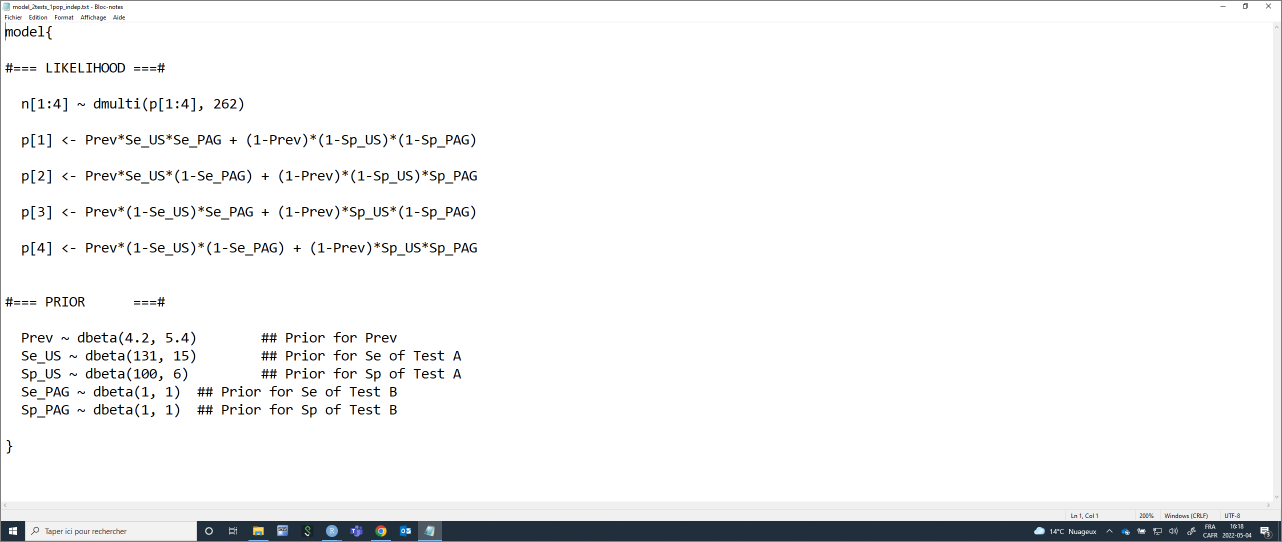
\includegraphics[keepaspectratio]{_main_files/Figures/model_2tests_1pop_indep.png}}
\caption{\textbf{Text file with the model for 2 independent diagnostic tests in 1 single population.}}
\end{figure}

\strut \\
We will also need to provide a list of initial values (one per Markov chain) for all unknown parameters.

\begin{Shaded}
\begin{Highlighting}[]
\CommentTok{\#Initializing values for the parameters Prev, and the Ses and Sps of the two tests for the 3 chains.}
\NormalTok{inits }\OtherTok{\textless{}{-}} \FunctionTok{list}\NormalTok{(}\FunctionTok{list}\NormalTok{(}\AttributeTok{Prev=}\FloatTok{0.50}\NormalTok{,}
              \AttributeTok{Se\_US=}\FloatTok{0.90}\NormalTok{,}
              \AttributeTok{Sp\_US=}\FloatTok{0.90}\NormalTok{,}
              \AttributeTok{Se\_PAG=}\FloatTok{0.90}\NormalTok{,}
              \AttributeTok{Sp\_PAG=}\FloatTok{0.90}\NormalTok{),}
              
              \FunctionTok{list}\NormalTok{(}\AttributeTok{Prev=}\FloatTok{0.70}\NormalTok{,}
              \AttributeTok{Se\_US=}\FloatTok{0.10}\NormalTok{,}
              \AttributeTok{Sp\_US=}\FloatTok{0.10}\NormalTok{,}
              \AttributeTok{Se\_PAG=}\FloatTok{0.10}\NormalTok{,}
              \AttributeTok{Sp\_PAG=}\FloatTok{0.10}\NormalTok{),}
              
              \FunctionTok{list}\NormalTok{(}\AttributeTok{Prev=}\FloatTok{0.50}\NormalTok{,}
              \AttributeTok{Se\_US=}\FloatTok{0.50}\NormalTok{,}
              \AttributeTok{Sp\_US=}\FloatTok{0.50}\NormalTok{,}
              \AttributeTok{Se\_PAG=}\FloatTok{0.50}\NormalTok{,}
              \AttributeTok{Sp\_PAG=}\FloatTok{0.50}\NormalTok{)}
\NormalTok{              )}
\end{Highlighting}
\end{Shaded}

Now we can run the model using \texttt{jags()} function.

\begin{Shaded}
\begin{Highlighting}[]
\FunctionTok{library}\NormalTok{(R2jags)}
\FunctionTok{library}\NormalTok{(coda)}

\CommentTok{\#Run the Bayesian model}
\NormalTok{bug.out }\OtherTok{\textless{}{-}} \FunctionTok{jags}\NormalTok{(}\AttributeTok{data=}\NormalTok{datalist,                             }
               \AttributeTok{model.file=}\StringTok{"model\_2tests\_1pop\_indep.txt"}\NormalTok{,     }
               \AttributeTok{parameters.to.save=}\FunctionTok{c}\NormalTok{(}\StringTok{"Prev"}\NormalTok{, }\StringTok{"Se\_US"}\NormalTok{, }\StringTok{"Sp\_US"}\NormalTok{, }\StringTok{"Se\_PAG"}\NormalTok{, }\StringTok{"Sp\_PAG"}\NormalTok{),               }
               \AttributeTok{n.chains=}\DecValTok{3}\NormalTok{,                                 }
               \AttributeTok{inits=}\NormalTok{inits,                                }
               \AttributeTok{n.iter=}\DecValTok{11000}\NormalTok{,                                }
               \AttributeTok{n.burnin=}\DecValTok{1000}\NormalTok{,                              }
               \AttributeTok{n.thin=}\DecValTok{1}\NormalTok{,                                   }
               \AttributeTok{DIC=}\ConstantTok{FALSE}\NormalTok{)                                   }
\end{Highlighting}
\end{Shaded}

\begin{verbatim}
## Compiling model graph
##    Resolving undeclared variables
##    Allocating nodes
## Graph information:
##    Observed stochastic nodes: 1
##    Unobserved stochastic nodes: 5
##    Total graph size: 32
## 
## Initializing model
\end{verbatim}

Then we could produce the diagnostic plots, compute the ESS, and print out our results as we did previously (results not shown).

\begin{Shaded}
\begin{Highlighting}[]
\FunctionTok{library}\NormalTok{(mcmcplots)}
\NormalTok{bug.mcmc }\OtherTok{\textless{}{-}} \FunctionTok{as.mcmc}\NormalTok{(bug.out)          }
\FunctionTok{mcmcplot}\NormalTok{(bug.mcmc, }\AttributeTok{title=}\StringTok{"Diagnostic plots"}\NormalTok{) }
\FunctionTok{effectiveSize}\NormalTok{(bug.mcmc)}
\FunctionTok{print}\NormalTok{(bug.out, }\AttributeTok{digits.summary=}\DecValTok{3}\NormalTok{) }
\end{Highlighting}
\end{Shaded}

Or we could ask to plot the prior and posterior distributions of one (or many) of the parameters. Here, we asked for the prior and posterior distributions of \emph{US} sensitivity.

\begin{Shaded}
\begin{Highlighting}[]
\CommentTok{\#Plot the posterior distribution}
\FunctionTok{plot}\NormalTok{(}\FunctionTok{density}\NormalTok{(}\AttributeTok{x=}\NormalTok{bug.out}\SpecialCharTok{$}\NormalTok{BUGSoutput}\SpecialCharTok{$}\NormalTok{sims.list}\SpecialCharTok{$}\NormalTok{Se\_US),      }
     \AttributeTok{main=}\StringTok{"US sensitivity"}\NormalTok{,                         }
     \AttributeTok{xlab=}\StringTok{"Sensitivity"}\NormalTok{, }\AttributeTok{ylab=}\StringTok{"Density"}\NormalTok{,                }
\NormalTok{     )}

\CommentTok{\#plot the prior distribution}
\FunctionTok{curve}\NormalTok{(}\FunctionTok{dbeta}\NormalTok{(x, }\AttributeTok{shape1=}\NormalTok{Se.TestA.shapea, }\AttributeTok{shape2=}\NormalTok{Se.TestA.shapeb), }\AttributeTok{from=}\DecValTok{0}\NormalTok{, }\AttributeTok{to=}\DecValTok{1}\NormalTok{,          }
      \AttributeTok{lty=}\DecValTok{2}\NormalTok{,                                                                   }
      \AttributeTok{col=}\StringTok{"red"}\NormalTok{,                                                                }
      \AttributeTok{add=}\ConstantTok{TRUE}\NormalTok{)                                                                }
\end{Highlighting}
\end{Shaded}

\begin{figure}
\centering
\pandocbounded{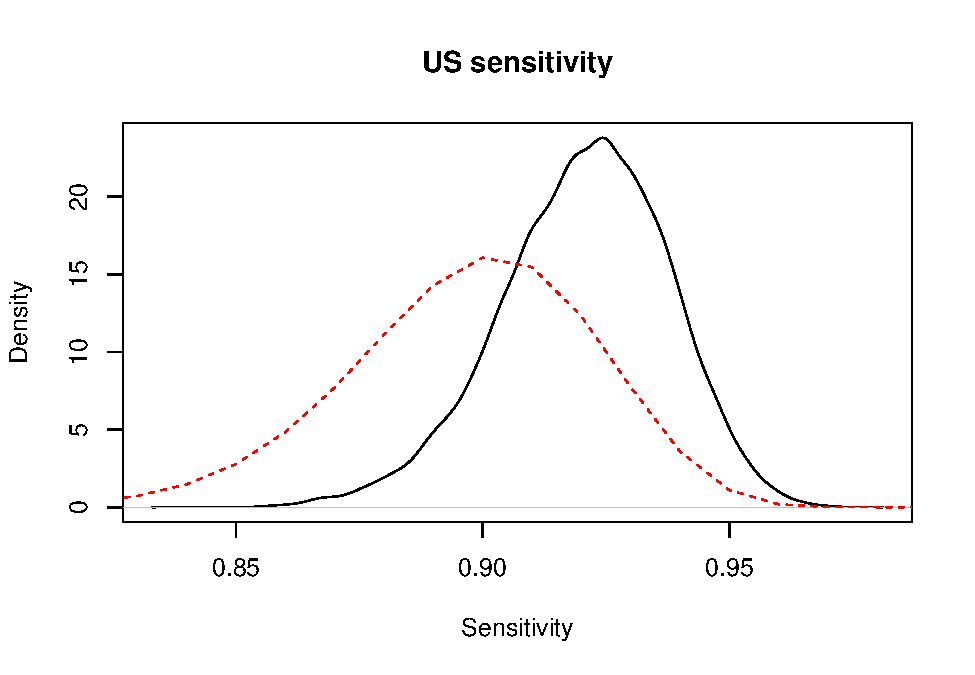
\includegraphics[keepaspectratio]{_main_files/_main_files/figure-latex/unnamed-chunk-37-1.pdf}}
\caption{\label{fig:unnamed-chunk-37}Prior (dashed red line) and posterior (full black line) distribution of US sensitivity.}
\end{figure}

\section{Allowing for conditional dependence}\label{allowing-for-conditional-dependence}

We will not go into the exact details, but \href{https://onlinelibrary.wiley.com/doi/10.1111/j.0006-341X.2001.00158.x}{Dendukuri and Joseph (2001)} developed a highly generalisable model structure that can account for conditional dependence between diagnostic tests. To allow for conditional dependence between tests, the likelihood function would be modified as follows, by adding covariance terms representing the conditional dependence between tests:

\(n[1:4] \sim dmulti(P[1:4], n)\)

\(P1 = P*(SeA*SeB+covp) + (1-P)*((1-SpA)*(1-SpB)+covn)\)\\
\(P2 = P*(SeA*(1-SeB)-covp) + (1-P)*((1-SpA)*SpB-covn)\)\\
\(P3 = P*((1-SeA)*SeB-covp) + (1-P)*(SpA*(1-SpB)-covn)\)\\
\(P3 = P*((1-SeA)*(1-SeB)+covp) + (1-P)*(SpA*SpB+covn)\)

Thus, a small quantity (\emph{covp}) is added to the sensitivities of the tests when they agree on a positive individual, and that same quantity is substracted when the tests disagree. \emph{covp} thus represents the positive covariance between tests. Similarly, \emph{covn} represents the negative covariance between tests. The effect of these covariances, if greater than zero, will be to penalize our estimates of the tests sensitivities and specificities to account for their conditional dependence. Note that having covariance terms equal to 0.0 (i.e., conditional independence) is a possibility. This model, therefore, \textbf{is not imposing a conditional dependence between tests, it rather allows for conditional dependence}.

Moreover, \href{https://onlinelibrary.wiley.com/doi/10.1111/j.0006-341X.2001.00158.x}{Dendukuri and Joseph (2001)} proposed constraints on these covariance terms based on the inferred test sensitivities and specificities. This latter aspect allows to specify ``natural limits'' for the covariance terms prior distributions. Briefly, they demonstrated that:

\begin{itemize}
\tightlist
\item
  \emph{covp} \textgreater{} \((1-SeA)*(SeB-1)\)\\
\item
  \emph{covp} \textless{} (the minimum between \(SeA\) and \(SeB\)) minus \(SeA*SeB\)\\
\item
  \emph{covn} \textgreater{} \((SpA-1)*(1-SpB)\)\\
\item
  \emph{covn} \textless{} (the minimum between \(SpA\) and \(SpB\)) minus \(SpA*SpB\)
\end{itemize}

Thus, we can use these as the minimum and maximum for \emph{covp} and \emph{covn}. For instance, we could use uniform distributions with these limits to describe the prior distributions for \emph{covp} and \emph{covn}. Our LCM would thus become:

\begin{Shaded}
\begin{Highlighting}[]
\CommentTok{\#Create the JAGS text file}
\NormalTok{model\_2tests\_1pop\_dep }\OtherTok{\textless{}{-}} \FunctionTok{paste0}\NormalTok{(}\StringTok{"model\{}

\StringTok{\#=== LIKELIHOOD ===\#}

\StringTok{  n[1:4] \textasciitilde{} dmulti(p[1:4], "}\NormalTok{,n,}\StringTok{")}
\StringTok{  p[1] \textless{}{-} Prev*(Se\_"}\NormalTok{, TestA, }\StringTok{"*Se\_"}\NormalTok{, TestB, }\StringTok{" + covp) + (1{-}Prev)*((1{-}Sp\_"}\NormalTok{, TestA, }\StringTok{")*(1{-}Sp\_"}\NormalTok{, TestB, }\StringTok{") + covn)}
\StringTok{  p[2] \textless{}{-} Prev*(Se\_"}\NormalTok{, TestA, }\StringTok{"*(1{-}Se\_"}\NormalTok{, TestB, }\StringTok{") {-} covp) + (1{-}Prev)*((1{-}Sp\_"}\NormalTok{, TestA, }\StringTok{")*Sp\_"}\NormalTok{, TestB, }\StringTok{" {-} covn)}
\StringTok{  p[3] \textless{}{-} Prev*((1{-}Se\_"}\NormalTok{, TestA, }\StringTok{")*Se\_"}\NormalTok{, TestB, }\StringTok{" {-} covp) + (1{-}Prev)*(Sp\_"}\NormalTok{, TestA, }\StringTok{"*(1{-}Sp\_"}\NormalTok{, TestB, }\StringTok{") {-} covn)}
\StringTok{  p[4] \textless{}{-} Prev*((1{-}Se\_"}\NormalTok{, TestA, }\StringTok{")*(1{-}Se\_"}\NormalTok{, TestB, }\StringTok{") + covp) + (1{-}Prev)*(Sp\_"}\NormalTok{, TestA, }\StringTok{"*Sp\_"}\NormalTok{, TestB, }\StringTok{" + covn)}

\StringTok{\#=== PRIOR  ===\#}

\StringTok{  Prev \textasciitilde{} dbeta("}\NormalTok{,Prev.shapea,}\StringTok{", "}\NormalTok{,Prev.shapeb,}\StringTok{")    \#\# Prior for Prev}
\StringTok{  Se\_"}\NormalTok{, TestA, }\StringTok{" \textasciitilde{} dbeta("}\NormalTok{,Se.TestA.shapea,}\StringTok{", "}\NormalTok{,Se.TestA.shapeb,}\StringTok{")  \#\# Prior for Se of Test A}
\StringTok{  Sp\_"}\NormalTok{, TestA, }\StringTok{" \textasciitilde{} dbeta("}\NormalTok{,Sp.TestA.shapea,}\StringTok{", "}\NormalTok{,Sp.TestA.shapeb,}\StringTok{")  \#\# Prior for Sp of Test A}
\StringTok{  Se\_"}\NormalTok{, TestB, }\StringTok{" \textasciitilde{} dbeta("}\NormalTok{,Se.TestB.shapea,}\StringTok{", "}\NormalTok{,Se.TestB.shapeb,}\StringTok{")  \#\# Prior for Se of Test B}
\StringTok{  Sp\_"}\NormalTok{, TestB, }\StringTok{" \textasciitilde{} dbeta("}\NormalTok{,Sp.TestB.shapea,}\StringTok{", "}\NormalTok{,Sp.TestB.shapeb,}\StringTok{")  \#\# Prior for Sp of Test B}
\StringTok{  }
\StringTok{\#=== CONDITIONAL DEPENDENCE STRUCTURE ===\#}

\StringTok{  covp \textasciitilde{} dunif(minp,maxp)}
\StringTok{  covn \textasciitilde{} dunif(minn,maxn)}
\StringTok{  minp \textless{}{-} (1{-}Se\_"}\NormalTok{, TestA, }\StringTok{")*(Se\_"}\NormalTok{, TestB, }\StringTok{"{-}1)}
\StringTok{  minn \textless{}{-} (Sp\_"}\NormalTok{, TestA, }\StringTok{"{-}1)*(1{-}Sp\_"}\NormalTok{, TestB, }\StringTok{")}
\StringTok{  maxp \textless{}{-} min(Se\_"}\NormalTok{, TestA, }\StringTok{",Se\_"}\NormalTok{, TestB, }\StringTok{") {-} Se\_"}\NormalTok{, TestA, }\StringTok{"*Se\_"}\NormalTok{, TestB, }\StringTok{"    }
\StringTok{  maxn \textless{}{-} min(Sp\_"}\NormalTok{, TestA, }\StringTok{",Sp\_"}\NormalTok{, TestB, }\StringTok{") {-} Sp\_"}\NormalTok{, TestA, }\StringTok{"*Sp\_"}\NormalTok{, TestB, }\StringTok{"  }
\StringTok{  }
\StringTok{\}"}\NormalTok{)}

\CommentTok{\#write as a text (.txt) file}
\FunctionTok{write.table}\NormalTok{(model\_2tests\_1pop\_dep, }
            \AttributeTok{file=}\StringTok{"model\_2tests\_1pop\_dep.txt"}\NormalTok{, }
            \AttributeTok{quote=}\ConstantTok{FALSE}\NormalTok{, }
            \AttributeTok{sep=}\StringTok{""}\NormalTok{, }
            \AttributeTok{row.names=}\ConstantTok{FALSE}\NormalTok{,}
             \AttributeTok{col.names=}\ConstantTok{FALSE}\NormalTok{)}
\end{Highlighting}
\end{Shaded}

Again, with this code, we could simply modify the labels for Test A and Test B, and the shape parameters for the prior distributions and the text file with the \texttt{JAGS} model will automatically be updated. Currently, it looks like this:

\begin{figure}
\centering
\pandocbounded{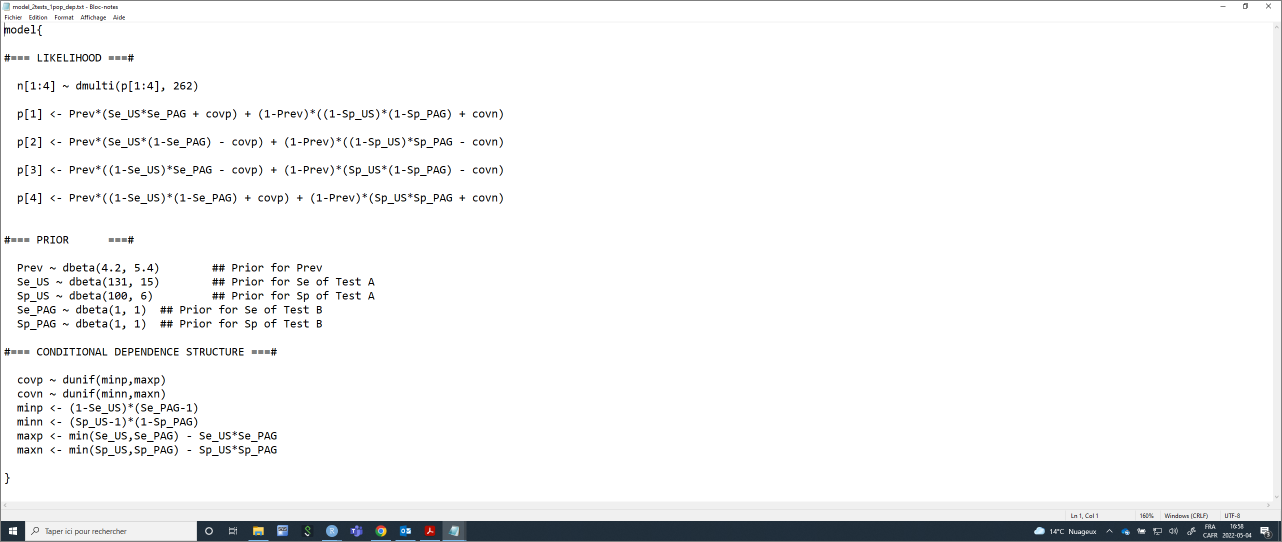
\includegraphics[keepaspectratio]{_main_files/Figures/model_2tests_1pop_dep.png}}
\caption{\textbf{Text file with the model for 2 possibly conditionally dependent diagnostic tests in 1 single population.}}
\end{figure}

\strut \\
If we do not modify the other priors nor the dataset used previously we could run this model using the \texttt{jags()} function. However, we now have to add initial values for \emph{covp} and \emph{covn}. Also, note that we have added \emph{covp} and \emph{covn} to the list of parameters that we would like to monitor and we have increased substantially the number of iterations. The model allowing for conditional dependence between tests tends to be more difficult to solve. We will thus need a substantial number of iterations to get a decent ESS.

\begin{Shaded}
\begin{Highlighting}[]
\CommentTok{\#Initializing values for the parameters Prev, and the Ses and Sps of the two tests for the 3 chains.}
\NormalTok{inits }\OtherTok{\textless{}{-}} \FunctionTok{list}\NormalTok{(}\FunctionTok{list}\NormalTok{(}\AttributeTok{Prev=}\FloatTok{0.50}\NormalTok{,}
              \AttributeTok{Se\_US=}\FloatTok{0.90}\NormalTok{,}
              \AttributeTok{Sp\_US=}\FloatTok{0.90}\NormalTok{,}
              \AttributeTok{Se\_PAG=}\FloatTok{0.90}\NormalTok{,}
              \AttributeTok{Sp\_PAG=}\FloatTok{0.90}\NormalTok{,}
              \AttributeTok{covp=}\DecValTok{0}\NormalTok{,}
              \AttributeTok{covn=}\DecValTok{0}\NormalTok{),}
              
              \FunctionTok{list}\NormalTok{(}\AttributeTok{Prev=}\FloatTok{0.70}\NormalTok{,}
              \AttributeTok{Se\_US=}\FloatTok{0.10}\NormalTok{,}
              \AttributeTok{Sp\_US=}\FloatTok{0.10}\NormalTok{,}
              \AttributeTok{Se\_PAG=}\FloatTok{0.10}\NormalTok{,}
              \AttributeTok{Sp\_PAG=}\FloatTok{0.10}\NormalTok{,}
              \AttributeTok{covp=}\FloatTok{0.01}\NormalTok{,}
              \AttributeTok{covn=}\FloatTok{0.01}\NormalTok{),}
              
              \FunctionTok{list}\NormalTok{(}\AttributeTok{Prev=}\FloatTok{0.50}\NormalTok{,}
              \AttributeTok{Se\_US=}\FloatTok{0.50}\NormalTok{,}
              \AttributeTok{Sp\_US=}\FloatTok{0.50}\NormalTok{,}
              \AttributeTok{Se\_PAG=}\FloatTok{0.50}\NormalTok{,}
              \AttributeTok{Sp\_PAG=}\FloatTok{0.50}\NormalTok{,}
              \AttributeTok{covp=}\FloatTok{0.05}\NormalTok{,}
              \AttributeTok{covn=}\FloatTok{0.05}\NormalTok{)}
\NormalTok{              )}


\FunctionTok{library}\NormalTok{(R2jags)}
\FunctionTok{library}\NormalTok{(coda)}

\CommentTok{\#Run the Bayesian model}
\NormalTok{bug.out }\OtherTok{\textless{}{-}} \FunctionTok{jags}\NormalTok{(}\AttributeTok{data=}\NormalTok{datalist,                             }
               \AttributeTok{model.file=}\StringTok{"model\_2tests\_1pop\_dep.txt"}\NormalTok{,     }
               \AttributeTok{parameters.to.save=}\FunctionTok{c}\NormalTok{(}\StringTok{"Prev"}\NormalTok{, }\StringTok{"Se\_US"}\NormalTok{, }\StringTok{"Sp\_US"}\NormalTok{, }\StringTok{"Se\_PAG"}\NormalTok{, }\StringTok{"Sp\_PAG"}\NormalTok{, }\StringTok{"covp"}\NormalTok{, }\StringTok{"covn"}\NormalTok{),               }
               \AttributeTok{n.chains=}\DecValTok{3}\NormalTok{,                                 }
               \AttributeTok{inits=}\NormalTok{inits,                                }
               \AttributeTok{n.iter=}\DecValTok{101000}\NormalTok{,                                }
               \AttributeTok{n.burnin=}\DecValTok{1000}\NormalTok{,                              }
               \AttributeTok{n.thin=}\DecValTok{1}\NormalTok{,                                   }
               \AttributeTok{DIC=}\ConstantTok{FALSE}\NormalTok{)                                   }
\end{Highlighting}
\end{Shaded}

\begin{verbatim}
## Compiling model graph
##    Resolving undeclared variables
##    Allocating nodes
## Graph information:
##    Observed stochastic nodes: 1
##    Unobserved stochastic nodes: 7
##    Total graph size: 58
## 
## Initializing model
\end{verbatim}

Then we could produce the diagnostic plots, compute the ESS, and print out our results as we did previously (the diagnostic plots are not shown).

\begin{Shaded}
\begin{Highlighting}[]
\FunctionTok{library}\NormalTok{(mcmcplots)}
\NormalTok{bug.mcmc }\OtherTok{\textless{}{-}} \FunctionTok{as.mcmc}\NormalTok{(bug.out)          }
\FunctionTok{mcmcplot}\NormalTok{(bug.mcmc, }\AttributeTok{title=}\StringTok{"Diagnostic plots"}\NormalTok{) }
\FunctionTok{effectiveSize}\NormalTok{(bug.mcmc)}
\FunctionTok{print}\NormalTok{(bug.out, }\AttributeTok{digits.summary=}\DecValTok{3}\NormalTok{) }
\end{Highlighting}
\end{Shaded}

\begin{Shaded}
\begin{Highlighting}[]
\FunctionTok{effectiveSize}\NormalTok{(bug.mcmc)}
\end{Highlighting}
\end{Shaded}

\begin{verbatim}
##      Prev    Se_PAG     Se_US    Sp_PAG     Sp_US      covn      covp 
## 15812.487  2167.916  6168.379  7883.295  6853.168  6822.977  2149.342
\end{verbatim}

\begin{Shaded}
\begin{Highlighting}[]
\FunctionTok{print}\NormalTok{(bug.out, }\AttributeTok{digits.summary=}\DecValTok{3}\NormalTok{) }
\end{Highlighting}
\end{Shaded}

\begin{verbatim}
## Inference for Bugs model at "model_2tests_1pop_dep.txt", fit using jags,
##  3 chains, each with 101000 iterations (first 1000 discarded)
##  n.sims = 300000 iterations saved. Running time = 6.46 secs
##        mu.vect sd.vect  2.5%   25%   50%   75% 97.5%  Rhat n.eff
## Prev     0.555   0.039 0.480 0.529 0.555 0.581 0.632 1.001 18000
## Se_PAG   0.949   0.035 0.872 0.925 0.954 0.979 0.998 1.002  2100
## Se_US    0.906   0.023 0.856 0.892 0.908 0.922 0.944 1.001  9700
## Sp_PAG   0.923   0.040 0.836 0.897 0.927 0.953 0.990 1.001 16000
## Sp_US    0.950   0.021 0.902 0.938 0.953 0.965 0.982 1.001 14000
## covn     0.033   0.020 0.002 0.018 0.031 0.045 0.077 1.001 22000
## covp     0.037   0.029 0.000 0.012 0.033 0.058 0.099 1.002  2000
## 
## For each parameter, n.eff is a crude measure of effective sample size,
## and Rhat is the potential scale reduction factor (at convergence, Rhat=1).
\end{verbatim}

The ESS is still just around 2,000 for some parameters (e.g., \emph{Se\_PAG}), if it was for publication, we would possibly let it run for more iterations.

The model proposed by \href{https://onlinelibrary.wiley.com/doi/10.1111/j.0006-341X.2001.00158.x}{Dendukuri and Joseph (2001)} can be used to model conditional dependence between two tests only. In Chapter 9 we will see that we can also used models where \textgreater{} 2 tests are compared (e.g., 3, 4, 5 tests). In such cases, the method described above could be used to evaluate pairwise dependence between tests (i.e., \emph{TestA vs.~TestB}, then \emph{TestA vs.~TestC}, and, finally, \emph{TestB vs.~TestC}).

\chapter{Exercise 2 - Two tests}\label{exercise-2---two-tests}

\section{Questions}\label{questions-1}

Open up the \texttt{R} project for Exercise 2 (i.e., the R project file named \emph{Exercise 2.Rproj}).

In the Exercise 2 folder, you will find partially completed \texttt{R} scripts. To answer the questions, try to complete the missing parts (they are highlighted by a \textbf{\#TO COMPLETE\#} comment). We also provided complete \texttt{R} scripts, but try to work it out on your own first!

\textbf{1. Start from the partially completed \emph{Question 1.R} script located in Exercise 2 folder.} We could try to estimate the Se and Sp of the PAG-based ELISA test when compared to US. We could, however, explicitly acknowledge that the US exam is not a gold-standard test. At first, we could assume that these tests are conditionally independent. We will use data from one population (herd \#1). In herd \#1, the cross-tabulated PAG by US results were as follows:

\textbf{Table.} Cross-classified results of the PAG and US tests in herd \#1.

\begin{longtable}[]{@{}cccc@{}}
\toprule\noalign{}
& \textbf{US+} & \textbf{US-} & \textbf{Total} \\
\midrule\noalign{}
\endhead
\bottomrule\noalign{}
\endlastfoot
\textbf{PAG+} & 138 & 10 & 148 \\
\textbf{PAG-} & 1 & 113 & 114 \\
\textbf{Total} & 139 & 123 & 262 \\
\end{longtable}

How many unknown parameters do you have to estimate and how many degrees of freedom do you have? Therefore, how many informative priors will you need? Estimate PAG's Se and Sp, and true pregnancy prevalence using informative priors on US' Se and Sp, and on pregnancy's prevalence. Compare your results to those of Exercise 1 (question 4) where you estimated PAG's Se and Sp, but assuming that US was a gold standard test.

\textbf{Some literature to help you with Informative priors:}\\
In 2006, \href{https://www.sciencedirect.com/science/article/pii/S0093691X06001543?via\%3Dihub}{Romano et al.} reported, for a US exam conducted between 28-45 days post-insemination:\\
-Se = 0.90 (95CI: 0.85, 0.95)\\
-Sp = 0.95 (95CI: 0.90, 0.97)

Moreover, in a recent study conducted on 30 Canadian herds they reported an expected pregnancy prevalence of 42\% with 97.5\% percentile of 74\%.

\textbf{2. Start from the \texttt{R} script that you completed in Question 1.} Now run the same model, but use vague priors on all unknown parameters. Do you think it will work? What do you observe regarding the Markov chains?

\textbf{3. Start from the partially completed \emph{Question 3.R} script located in Exercise 2 folder.} Now, we could consider that some conditional dependency exist between the two tests. For instance, it was reported that PAG concentration is higher in first parity cows (\href{https://doi.org/10.3168/jds.2014-8974}{Ricci et al., 2015}, \href{https://doi.org/10.3168/jds.2015-10595}{Mercadante et al., 2016}). US exams may also be easier to
conduct on first parity cows and, thus, Se of both tests may be higher in first parity cows and lower in older cows. Build a model where conditional dependency is a possibility. How many unknown parameters and degrees of freedom do you have? Are your Markov chains behaving OK? What do you observe? Try to play with the number of iterations to reach an effective sample size (\textbf{ESS}) \textgreater{} 3,000. How are your results differing from that of question 1 (where you assumed conditional independence)?

\section{Answers}\label{answers-1}

\textbf{1.} We could try to estimate the Se and Sp of the PAG-based ELISA test using US as comparison. We could, however, explicitly acknowledge that the US exam is not a gold-standard test. At first, we could assume that these tests are conditionally independent. How many unknown parameters do you have to estimate and how many degrees of freedom do you have? Therefore, how many informative priors will you need? Estimate PAG's Se and Sp, and true pregnancy prevalence using informative priors on US' Se and Sp, and on pregnancy's prevalence. Compare your results to those of Exercise 1 (question 4) where you estimated PAG's Se and Sp, but assuming that US was a gold standard test.

\textbf{Answer:} We now have 5 unknown parameters (PAG's \emph{Se} and \emph{Sp}, US' \emph{Se} and \emph{Sp}, and pregnancy prevalence, \emph{P}) and we have 3 degrees of freedom (i.e., one 2x2 table where three cells are providing valuable information and the content of the 4th cell can be deduced from the total number of observations minus the content of the other three cells). Thus, we need informative priors for at least 2 parameters. As suggested, we will use informative priors for 3 parameters ( US' \emph{Se} and \emph{Sp}, and \emph{P}), so the model is identifiable.

\textbf{Table.} Results assuming \textbf{US is not perfect}

\begin{longtable}[]{@{}ccc@{}}
\toprule\noalign{}
\textbf{Parameters} & \textbf{Median} & \textbf{95CI} \\
\midrule\noalign{}
\endhead
\bottomrule\noalign{}
\endlastfoot
\textbf{PAG Se} & 0.993 & 0.968, 1.000 \\
\textbf{PAG Sp} & 0.979 & 0.922, 0.999 \\
\textbf{US Se} & 0.923 & 0.885, 0.955 \\
\textbf{US Sp} & 0.970 & 0.941, 0.987 \\
\textbf{Prevalence} & 0.554 & 0.493, 0.614 \\
\end{longtable}

As a comparison, in question 4 of Exercise 1, where we considered that US was a perfect test, we assumed that US \emph{Se} and \emph{Sp} was 1.0 and we estimated accuracy of PAG as:

\textbf{Table.} Results assuming \textbf{US is perfect}

\begin{longtable}[]{@{}ccc@{}}
\toprule\noalign{}
\textbf{Parameters} & \textbf{Median} & \textbf{95CI} \\
\midrule\noalign{}
\endhead
\bottomrule\noalign{}
\endlastfoot
\textbf{PAG Se} & 0.988 & 0.961, 0.998 \\
\textbf{PAG Sp} & 0.915 & 0.859, 0.955 \\
\end{longtable}

Thus, the 10 cows that were PAG+ and US- where all considered to be a failure of the PAG test (i.e., False+ on PAG). This resulted in a lower estimated PAG specificity. Now that we indicated that US is not perfect, these disagreements are not exclusively attributed to the PAG test, hence the higher estimated PAG specificity.

\textbf{2.} Now run the same model, but use vague priors on all unknown parameters. Do you think it will work? What do you observe regarding the Markov chains?

\textbf{Answer:} Beforehand, we would say no, it will not work! We have 5 unknown parameters and only 3 degrees of freedom. The model is non-identifiable. With some data sets, though, it will sometimes work (if the number of potential solutions is very limited). This is the case here, there is so little disagreement between tests that the Markov chains were able to converge. However, they have a strange behaviour, for all parameters, we always have two chains converging in one area and another one converging at the exact opposite (see figure below). This is a case where we have a mirror solution. When such situation arise, we could consider adding informative priors for at least one other parameter (to make the model identifiable). However, remember that \textbf{mirror solutions may arise even in LCM that are identifiable}. In this latter case, we would have to exclude the Markov chain producing the ``biologically impossible'' results or to modify the set of initial values of the problematic Markov chain.

\begin{figure}
\centering
\pandocbounded{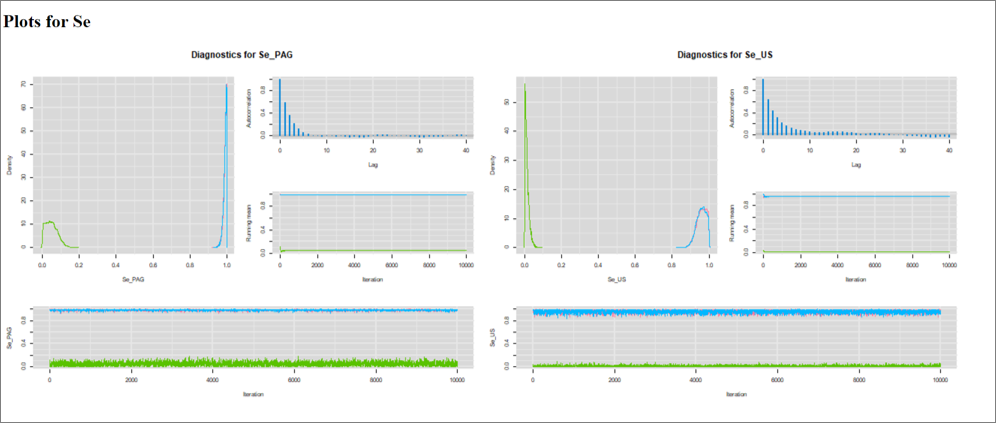
\includegraphics[keepaspectratio]{_main_files/Figures/mirror.png}}
\caption{\textbf{Diagnostic plot - Mirror solution}}
\end{figure}

\strut \\
\textbf{3.} Build a model where conditional dependency is a possibility. How many unknown parameters and degrees of freedom do you have? Are your Markov chains behaving OK? What do you observe? Try to play with the number of iterations to reach an effective sample size (\textbf{ESS}) \textgreater{} 3,000. How are your results differing from that of question 1 (where you assumed conditional independence)?

\textbf{Answer:} We have 7 unkown parameters (PAG's \emph{Se} and \emph{Sp}, US' \emph{Se} and \emph{Sp}, \emph{P}, \emph{covp}, and \emph{covn}). We still only have 3 degrees of freedom, so we need informative priors on 4 parameters. We can use the \href{https://www.sciencedirect.com/science/article/pii/S0093691X06001543?via\%3Dihub}{Romano et al.~(2006)} derived priors for US' \emph{Se} and \emph{Sp}, and use our pregnancy prevalence informative prior. We can use the natural bounds of \emph{covp} and \emph{covn} proposed by \href{https://onlinelibrary.wiley.com/doi/10.1111/j.0006-341X.2001.00158.x}{Dendukuri and Joseph (2001)} as priors for these parameters.

We initially ran the LCM for 11,000 iterations (with a burn-in of 1,000). The Markov chains were still cycling up and down for some of the parameters (\emph{Se\_PAG} and \emph{covp} were the worst; see \emph{Se\_PAG} below). But it is still cycling in a very tight space (i.e., check the Y-axis scale). Autocorrelation seems to be a problem (especially for \emph{Se\_pag} and \emph{covp}, again).

\begin{figure}
\centering
\pandocbounded{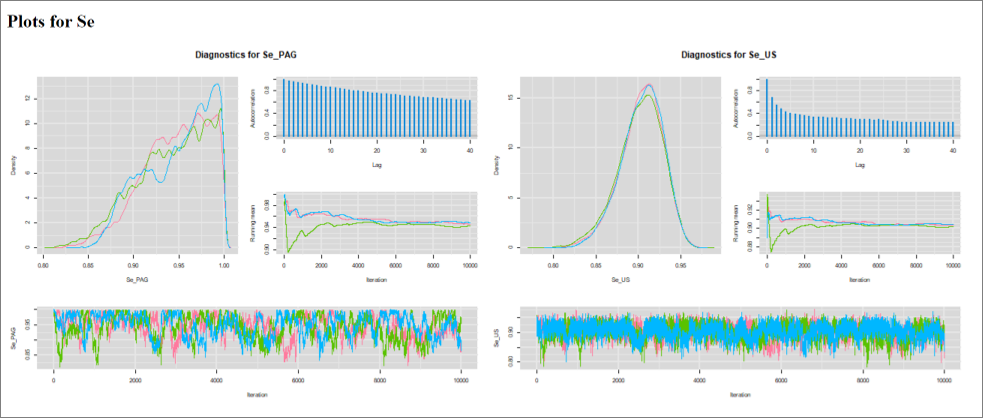
\includegraphics[keepaspectratio]{_main_files/Figures/Ex2 Q3 11000 it.png}}
\caption{\textbf{Diagnostic plot - 11,000 iterations}}
\end{figure}

\strut \\
The ESS for these two parameters were both around 170. So, despite the 30,000 values (3 chains times 11,000 iterations, minus the 1,000 burn-in of each chain) stored during the Monte Carlo simulation, there is just the equivalent of 170 independent values. This would be quite a small sample to report with precision the median, 2.5th, and 97.5th estimates. Using the exact same model, but with a number of iteration of 201,000, we obtained ESS \textgreater3,500 for all parameters.

\textbf{Table.} Results of the LCM assuming or not conditional independence between diagnostic tests.

\begin{longtable}[]{@{}
  >{\centering\arraybackslash}p{(\linewidth - 10\tabcolsep) * \real{0.1416}}
  >{\centering\arraybackslash}p{(\linewidth - 10\tabcolsep) * \real{0.3009}}
  >{\centering\arraybackslash}p{(\linewidth - 10\tabcolsep) * \real{0.1239}}
  >{\centering\arraybackslash}p{(\linewidth - 10\tabcolsep) * \real{0.0265}}
  >{\centering\arraybackslash}p{(\linewidth - 10\tabcolsep) * \real{0.2832}}
  >{\centering\arraybackslash}p{(\linewidth - 10\tabcolsep) * \real{0.1239}}@{}}
\toprule\noalign{}
\begin{minipage}[b]{\linewidth}\centering
\end{minipage} & \begin{minipage}[b]{\linewidth}\centering
\textbf{Conditional independence LCM}
\end{minipage} & \begin{minipage}[b]{\linewidth}\centering
\end{minipage} & \begin{minipage}[b]{\linewidth}\centering
\end{minipage} & \begin{minipage}[b]{\linewidth}\centering
\textbf{Conditional dependence LCM}
\end{minipage} & \begin{minipage}[b]{\linewidth}\centering
\end{minipage} \\
\midrule\noalign{}
\endhead
\bottomrule\noalign{}
\endlastfoot
\textbf{Parameters} & \textbf{Median} & \textbf{95CI} & & \textbf{Median} & \textbf{95CI} \\
\textbf{PAG Se} & 0.993 & 0.968, 1.00 & & 0.952 & 0.866, 0.998 \\
\textbf{PAG Sp} & 0.979 & 0.922, 0.999 & & 0.924 & 0.833, 0.988 \\
\textbf{US Se} & 0.923 & 0.885, 0.955 & & 0.906 & 0.847, 0.947 \\
\textbf{US Sp} & 0.970 & 0.941, 0.987 & & 0.951 & 0.899, 0.981 \\
\textbf{covp} & NA & NA & & 0.035 & 0.000, 0.104 \\
\textbf{covn} & NA & NA & & 0.032 & 0.002, 0.079 \\
\textbf{Prevalence} & 0.554 & 0.493, 0.614 & & 0.555 & 0.479, 0.634 \\
\end{longtable}

When we compare the LCM assuming conditional independence \emph{vs.} the one allowing conditional dependence, we can see that the tests' Se and Sp estimates are slightly lower in the model allowing conditional dependence. Indeed, in that model the covariance terms, \emph{covp} and \emph{covn}, where small, but positive. Remember, in the model allowing for conditional dependence, the agreement between tests is now due to the PAG and US accuracy parameters (e.g., their Se) \textbf{plus a small value} due to their covariance (e.g., \emph{covp}). Therefore, the tests accuracy parameters estimates will be reduced as their covariance is increased.

\chapter{Multiple populations}\label{multiple-populations}

In some situations, the diagnostic tests will be apply to two or more populations with different disease prevalence. In such cases, it could be reasonable to assume that:

\begin{itemize}
\tightlist
\item
  The prevalence varies from one population to another\\
\item
  The tests Se and Sp are constant across populations
\end{itemize}

It could then be advantageous to model the different populations simultaneously in the same LCM as described by \href{https://www.jstor.org/stable/2530508?seq=1}{Hui and Walter (1980)}. With two populations, we would have six unknown parameters (\emph{SeA} and \emph{SpA}, \emph{SeB} and \emph{SpB}, and each population's prevalence, \emph{P1} and \emph{P2}). When conducting two diagnostic tests in two populations, the data generated can be presented as two 2x2 tables presenting the cross-classified results of the two tests.

\textbf{Table.} Cross-classified results from two diagnostic tests in two populations.

\begin{longtable}[]{@{}
  >{\centering\arraybackslash}p{(\linewidth - 12\tabcolsep) * \real{0.1731}}
  >{\centering\arraybackslash}p{(\linewidth - 12\tabcolsep) * \real{0.1250}}
  >{\centering\arraybackslash}p{(\linewidth - 12\tabcolsep) * \real{0.1250}}
  >{\centering\arraybackslash}p{(\linewidth - 12\tabcolsep) * \real{0.1538}}
  >{\centering\arraybackslash}p{(\linewidth - 12\tabcolsep) * \real{0.1731}}
  >{\centering\arraybackslash}p{(\linewidth - 12\tabcolsep) * \real{0.1250}}
  >{\centering\arraybackslash}p{(\linewidth - 12\tabcolsep) * \real{0.1250}}@{}}
\toprule\noalign{}
\begin{minipage}[b]{\linewidth}\centering
\textbf{Population 1}
\end{minipage} & \begin{minipage}[b]{\linewidth}\centering
\end{minipage} & \begin{minipage}[b]{\linewidth}\centering
\end{minipage} & \begin{minipage}[b]{\linewidth}\centering
\end{minipage} & \begin{minipage}[b]{\linewidth}\centering
\textbf{Population 2}
\end{minipage} & \begin{minipage}[b]{\linewidth}\centering
\end{minipage} & \begin{minipage}[b]{\linewidth}\centering
\end{minipage} \\
\midrule\noalign{}
\endhead
\bottomrule\noalign{}
\endlastfoot
& \textbf{Test A+} & \textbf{Test A-} & & & \textbf{Test A+} & \textbf{Test A-} \\
\textbf{Test B+} & Pop1 n1 & Pop1 n3 & & \textbf{Test B+} & Pop2 n1 & Pop2 n3 \\
\textbf{Test B-} & Pop1 n2 & Pop1 n4 & & \textbf{Test B-} & Pop2 n2 & Pop2 n4 \\
\end{longtable}

We can see from these 2x2 tables that we have 6 degrees of freedom available. Indeed, in each of the 2x2 table, we have three cells that do contribute a valuable information and the information in the 4th cell can be ``guessed'' using the total number of observations minus the content of the other three cells. The model proposed by \href{https://www.jstor.org/stable/2530508?seq=1}{Hui and Walter (1980)} is, therefore, barely identifiable.

\href{https://doi.org/10.20506/rst.40.1.3224}{Cheung et al.~(2021)} have described how the number of unknown parameters and degrees of freedom vary as function of the number of populations studied when comparing two conditionally independent diagnostic tests (see below).

\textbf{Table.} Number of degrees of freedom and of unknown parameters when comparing two conditionally independent diagnostic tests across various number of populations (adapted from \href{https://doi.org/10.20506/rst.40.1.3224}{Cheung et al.~(2021)}).

\begin{longtable}[]{@{}
  >{\centering\arraybackslash}p{(\linewidth - 6\tabcolsep) * \real{0.1753}}
  >{\centering\arraybackslash}p{(\linewidth - 6\tabcolsep) * \real{0.2532}}
  >{\centering\arraybackslash}p{(\linewidth - 6\tabcolsep) * \real{0.2532}}
  >{\centering\arraybackslash}p{(\linewidth - 6\tabcolsep) * \real{0.3182}}@{}}
\toprule\noalign{}
\begin{minipage}[b]{\linewidth}\centering
\textbf{Number of Populations}
\end{minipage} & \begin{minipage}[b]{\linewidth}\centering
\textbf{Number of unknown parameters (np)}
\end{minipage} & \begin{minipage}[b]{\linewidth}\centering
\textbf{Number of degrees of freedom (df)}
\end{minipage} & \begin{minipage}[b]{\linewidth}\centering
\textbf{Minimum number of informative priors needed}
\end{minipage} \\
\midrule\noalign{}
\endhead
\bottomrule\noalign{}
\endlastfoot
1 & 5 & 3 & 2 \\
2 & 6 & 6 & 0 \\
3 & 7 & 9 & 0 \\
4 & 8 & 12 & 0 \\
p & 4+p & 3*p & if df \textless{} np, then np-df \\
\end{longtable}

\section{Likelihood function with 2 populations}\label{likelihood-function-with-2-populations}

With two populations, the likelihood function that could be used to link the observed data (\emph{Pop1 n1}, \emph{Pop1 n2}, \ldots, \emph{Pop2 n4}) to the unknown parameters (\emph{SeA} and \emph{SpA}, \emph{SeB} and \emph{SpB}, and \emph{P1} and \emph{P2}) can be described as follows:

\(Ppop1[1:4] \sim dmulti(Pop1[1:4], nPop1)\)\\
\(Ppop1_1 = P1*SeA*SeB + (1-P1)*(1-SpA)*(1-SpB)\)\\
\(Ppop1_2 = P1*SeA*(1-SeB) + (1-P1)*(1-SpA)*SpB\)\\
\(Ppop1_3 = P1*(1-SeA)*SeB + (1-P1)*SpA*(1-SpB)\)\\
\(Ppop1_4 = P1*(1-SeA)*(1-SeB) + (1-P1)*SpA*SpB\)

\(Ppop2[1:4] \sim dmulti(Pop2[1:4], nPop2)\)\\
\(Ppop2_1 = P2*SeA*SeB + (1-P2)*(1-SpA)*(1-SpB)\)\\
\(Ppop2_2 = P2*SeA*(1-SeB) + (1-P2)*(1-SpA)*SpB\)\\
\(Ppop2_3 = P2*(1-SeA)*SeB + (1-P2)*SpA*(1-SpB)\)\\
\(Ppop2_4 = P2*(1-SeA)*(1-SeB) + (1-P2)*SpA*SpB\)

Where \(Ppop1_1\) to \(Ppop1_4\) and \(Ppop2_1\) to \(Ppop2_4\) are the probabilities of falling in a given cell of the 2x2 table in population 1 and population 2, respectively; and \(nPop1\) and \(nPop2\) are the number of individuals tested in population 1 and 2, respectively. Thus, if you look carefully, \textbf{we simply duplicated the likelihood function used before and we added subscripts to differentiate the cells, probabilities, and disease prevalence of the two populations.} Pretty cool right? If you have three, four, etc populations, you can then extend the likelihood function to include them.

\section{Organizing the data with 2 populations}\label{organizing-the-data-with-2-populations}

To run such a model, we simply need to provide, for each population, a dataset where \emph{n1}, \emph{n2}, \emph{n3}, and \emph{n4} are listed (in that order). For instance, if we use herd \#1 and herd \#2 from the PAG \emph{vs.} US study, we will have the following 2x2 tables:

\textbf{Table.} Cross-classified results from the PAG and US diagnostic tests in herd \#1 and herd \#2.

\begin{longtable}[]{@{}
  >{\centering\arraybackslash}p{(\linewidth - 16\tabcolsep) * \real{0.1277}}
  >{\centering\arraybackslash}p{(\linewidth - 16\tabcolsep) * \real{0.0957}}
  >{\centering\arraybackslash}p{(\linewidth - 16\tabcolsep) * \real{0.0957}}
  >{\centering\arraybackslash}p{(\linewidth - 16\tabcolsep) * \real{0.1170}}
  >{\centering\arraybackslash}p{(\linewidth - 16\tabcolsep) * \real{0.1277}}
  >{\centering\arraybackslash}p{(\linewidth - 16\tabcolsep) * \real{0.1277}}
  >{\centering\arraybackslash}p{(\linewidth - 16\tabcolsep) * \real{0.0957}}
  >{\centering\arraybackslash}p{(\linewidth - 16\tabcolsep) * \real{0.0957}}
  >{\centering\arraybackslash}p{(\linewidth - 16\tabcolsep) * \real{0.1170}}@{}}
\toprule\noalign{}
\begin{minipage}[b]{\linewidth}\centering
\textbf{Herd 1}
\end{minipage} & \begin{minipage}[b]{\linewidth}\centering
\end{minipage} & \begin{minipage}[b]{\linewidth}\centering
\end{minipage} & \begin{minipage}[b]{\linewidth}\centering
\textbf{Total}
\end{minipage} & \begin{minipage}[b]{\linewidth}\centering
\end{minipage} & \begin{minipage}[b]{\linewidth}\centering
\textbf{Herd 2}
\end{minipage} & \begin{minipage}[b]{\linewidth}\centering
\end{minipage} & \begin{minipage}[b]{\linewidth}\centering
\end{minipage} & \begin{minipage}[b]{\linewidth}\centering
\textbf{Total}
\end{minipage} \\
\midrule\noalign{}
\endhead
\bottomrule\noalign{}
\endlastfoot
& \textbf{US+} & \textbf{US-} & & & & \textbf{US+} & \textbf{US-} & \\
\textbf{PAG+} & 138 & 10 & & & \textbf{PAG+} & 71 & 8 & \\
\textbf{PAG-} & 1 & 113 & & & \textbf{PAG-} & 0 & 69 & \\
\textbf{Total} & & & 262 & & \textbf{Total} & & & 148 \\
\end{longtable}

The dataset could, thus be created as follows:

\begin{Shaded}
\begin{Highlighting}[]
\CommentTok{\#n is of the form : (TestA pos and TestB pos), (TestA pos and TestB neg), (TestA neg and TestB pos), then (TestA neg and TestB neg)}
\NormalTok{datalist }\OtherTok{\textless{}{-}} \FunctionTok{list}\NormalTok{(}\AttributeTok{Pop1=}\FunctionTok{c}\NormalTok{(}\DecValTok{138}\NormalTok{,}\DecValTok{1}\NormalTok{,}\DecValTok{10}\NormalTok{,}\DecValTok{113}\NormalTok{),}
                 \AttributeTok{Pop2=}\FunctionTok{c}\NormalTok{(}\DecValTok{71}\NormalTok{, }\DecValTok{0}\NormalTok{, }\DecValTok{8}\NormalTok{, }\DecValTok{69}\NormalTok{)}
\NormalTok{                 )}
\end{Highlighting}
\end{Shaded}

\section{The JAGS model with 2 populations}\label{the-jags-model-with-2-populations}

We could provide the values that will be used to described the prior distributions as we did before (so they are included in the model text file). The only difference is that we now have two prevalence parameters (\emph{P1} and \emph{P2}) to describe. In the example below, I will use vague priors for all parameters (just because we can!).

\begin{Shaded}
\begin{Highlighting}[]
\CommentTok{\#We could first create labels for TestA and TestB}
\NormalTok{TestA }\OtherTok{\textless{}{-}} \StringTok{"US"}
\NormalTok{TestB }\OtherTok{\textless{}{-}} \StringTok{"PAG"}

\CommentTok{\#Provide information for the prior distributions (all beta distributions) for the 6 unknown parameters }
\NormalTok{Prev1.shapea }\OtherTok{\textless{}{-}} \DecValTok{1}         \CommentTok{\#a shape parameter for Prev in population 1    }
\NormalTok{Prev1.shapeb }\OtherTok{\textless{}{-}} \DecValTok{1}         \CommentTok{\#b shape parameter for Prev in population 1}

\NormalTok{Prev2.shapea }\OtherTok{\textless{}{-}} \DecValTok{1}         \CommentTok{\#a shape parameter for Prev in population 2    }
\NormalTok{Prev2.shapeb }\OtherTok{\textless{}{-}} \DecValTok{1}         \CommentTok{\#b shape parameter for Prev in population 2}

\NormalTok{Se.TestA.shapea }\OtherTok{\textless{}{-}} \DecValTok{1}     \CommentTok{\#a shape parameter for Se of TestA}
\NormalTok{Se.TestA.shapeb }\OtherTok{\textless{}{-}} \DecValTok{1}     \CommentTok{\#b shape parameter for Se of TestA}
\NormalTok{Sp.TestA.shapea }\OtherTok{\textless{}{-}} \DecValTok{1}     \CommentTok{\#a shape parameter for Sp of TestA}
\NormalTok{Sp.TestA.shapeb }\OtherTok{\textless{}{-}} \DecValTok{1}     \CommentTok{\#b shape parameter for Sp of TestA}

\NormalTok{Se.TestB.shapea }\OtherTok{\textless{}{-}} \DecValTok{1}     \CommentTok{\#a shape parameter for Se of TestB}
\NormalTok{Se.TestB.shapeb }\OtherTok{\textless{}{-}} \DecValTok{1}     \CommentTok{\#b shape parameter for Se of TestB}
\NormalTok{Sp.TestB.shapea }\OtherTok{\textless{}{-}} \DecValTok{1}     \CommentTok{\#a shape parameter for Sp of TestB}
\NormalTok{Sp.TestB.shapeb }\OtherTok{\textless{}{-}} \DecValTok{1}     \CommentTok{\#b shape parameter for Sp of TestB}

\CommentTok{\#We will also need the total number of individuals tested in each population (nPop1 and nPop2)}
\NormalTok{n }\OtherTok{\textless{}{-}} \FunctionTok{sapply}\NormalTok{(datalist, sum)}
\NormalTok{nPop1 }\OtherTok{\textless{}{-}}\NormalTok{ n[}\DecValTok{1}\NormalTok{]}
\NormalTok{nPop2 }\OtherTok{\textless{}{-}}\NormalTok{ n[}\DecValTok{2}\NormalTok{]}
\end{Highlighting}
\end{Shaded}

With that, we have everything that is needed to write the \texttt{JAGS} model.

\begin{Shaded}
\begin{Highlighting}[]
\CommentTok{\#Create the JAGS text file}
\NormalTok{model\_2tests\_2pop\_indep }\OtherTok{\textless{}{-}} \FunctionTok{paste0}\NormalTok{(}\StringTok{"model\{}

\StringTok{\#=== LIKELIHOOD ===\#}

\StringTok{  \#=== POPULATION 1 ===\#}
\StringTok{  Pop1[1:4] \textasciitilde{} dmulti(p1[1:4], "}\NormalTok{,nPop1,}\StringTok{")}
\StringTok{  p1[1] \textless{}{-} Prev1*Se\_"}\NormalTok{, TestA, }\StringTok{"*Se\_"}\NormalTok{, TestB, }\StringTok{" + (1{-}Prev1)*(1{-}Sp\_"}\NormalTok{, TestA, }\StringTok{")*(1{-}Sp\_"}\NormalTok{, TestB, }\StringTok{")}
\StringTok{  p1[2] \textless{}{-} Prev1*Se\_"}\NormalTok{, TestA, }\StringTok{"*(1{-}Se\_"}\NormalTok{, TestB, }\StringTok{") + (1{-}Prev1)*(1{-}Sp\_"}\NormalTok{, TestA, }\StringTok{")*Sp\_"}\NormalTok{, TestB, }\StringTok{"}
\StringTok{  p1[3] \textless{}{-} Prev1*(1{-}Se\_"}\NormalTok{, TestA, }\StringTok{")*Se\_"}\NormalTok{, TestB, }\StringTok{" + (1{-}Prev1)*Sp\_"}\NormalTok{, TestA, }\StringTok{"*(1{-}Sp\_"}\NormalTok{, TestB, }\StringTok{")}
\StringTok{  p1[4] \textless{}{-} Prev1*(1{-}Se\_"}\NormalTok{, TestA, }\StringTok{")*(1{-}Se\_"}\NormalTok{, TestB, }\StringTok{") + (1{-}Prev1)*Sp\_"}\NormalTok{, TestA, }\StringTok{"*Sp\_"}\NormalTok{, TestB, }\StringTok{"}

\StringTok{  \#=== POPULATION 2 ===\#  }
\StringTok{  Pop2[1:4] \textasciitilde{} dmulti(p2[1:4], "}\NormalTok{,nPop2,}\StringTok{")}
\StringTok{  p2[1] \textless{}{-} Prev2*Se\_"}\NormalTok{, TestA, }\StringTok{"*Se\_"}\NormalTok{, TestB, }\StringTok{" + (1{-}Prev2)*(1{-}Sp\_"}\NormalTok{, TestA, }\StringTok{")*(1{-}Sp\_"}\NormalTok{, TestB, }\StringTok{")}
\StringTok{  p2[2] \textless{}{-} Prev2*Se\_"}\NormalTok{, TestA, }\StringTok{"*(1{-}Se\_"}\NormalTok{, TestB, }\StringTok{") + (1{-}Prev2)*(1{-}Sp\_"}\NormalTok{, TestA, }\StringTok{")*Sp\_"}\NormalTok{, TestB, }\StringTok{"}
\StringTok{  p2[3] \textless{}{-} Prev2*(1{-}Se\_"}\NormalTok{, TestA, }\StringTok{")*Se\_"}\NormalTok{, TestB, }\StringTok{" + (1{-}Prev2)*Sp\_"}\NormalTok{, TestA, }\StringTok{"*(1{-}Sp\_"}\NormalTok{, TestB, }\StringTok{")}
\StringTok{  p2[4] \textless{}{-} Prev2*(1{-}Se\_"}\NormalTok{, TestA, }\StringTok{")*(1{-}Se\_"}\NormalTok{, TestB, }\StringTok{") + (1{-}Prev2)*Sp\_"}\NormalTok{, TestA, }\StringTok{"*Sp\_"}\NormalTok{, TestB, }\StringTok{"}
\StringTok{  }
\StringTok{  }
\StringTok{\#=== PRIOR  ===\#}

\StringTok{  Prev1 \textasciitilde{} dbeta("}\NormalTok{,Prev1.shapea,}\StringTok{", "}\NormalTok{,Prev1.shapeb,}\StringTok{")     \#\# Prior for Prevalence in population 1}
\StringTok{  Prev2 \textasciitilde{} dbeta("}\NormalTok{,Prev2.shapea,}\StringTok{", "}\NormalTok{,Prev2.shapeb,}\StringTok{")     \#\# Prior for Prevalence in population 2}
\StringTok{  Se\_"}\NormalTok{, TestA, }\StringTok{" \textasciitilde{} dbeta("}\NormalTok{,Se.TestA.shapea,}\StringTok{", "}\NormalTok{,Se.TestA.shapeb,}\StringTok{")  \#\# Prior for Se of Test A}
\StringTok{  Sp\_"}\NormalTok{, TestA, }\StringTok{" \textasciitilde{} dbeta("}\NormalTok{,Sp.TestA.shapea,}\StringTok{", "}\NormalTok{,Sp.TestA.shapeb,}\StringTok{")  \#\# Prior for Sp of Test A}
\StringTok{  Se\_"}\NormalTok{, TestB, }\StringTok{" \textasciitilde{} dbeta("}\NormalTok{,Se.TestB.shapea,}\StringTok{", "}\NormalTok{,Se.TestB.shapeb,}\StringTok{")  \#\# Prior for Se of Test B}
\StringTok{  Sp\_"}\NormalTok{, TestB, }\StringTok{" \textasciitilde{} dbeta("}\NormalTok{,Sp.TestB.shapea,}\StringTok{", "}\NormalTok{,Sp.TestB.shapeb,}\StringTok{")  \#\# Prior for Sp of Test B}
\StringTok{  }
\StringTok{\}"}\NormalTok{)}

\CommentTok{\#write as a text (.txt) file}
\FunctionTok{write.table}\NormalTok{(model\_2tests\_2pop\_indep, }
            \AttributeTok{file=}\StringTok{"model\_2tests\_2pop\_indep.txt"}\NormalTok{, }
            \AttributeTok{quote=}\ConstantTok{FALSE}\NormalTok{, }
            \AttributeTok{sep=}\StringTok{""}\NormalTok{, }
            \AttributeTok{row.names=}\ConstantTok{FALSE}\NormalTok{,}
            \AttributeTok{col.names=}\ConstantTok{FALSE}\NormalTok{)}
\end{Highlighting}
\end{Shaded}

With this code, you could, again, simply modify the labels for Test A and Test B, and the shape parameters for the prior distributions. The text file with the \texttt{JAGS} model will automatically be updated. Currently, it looks like this:

\begin{figure}
\centering
\pandocbounded{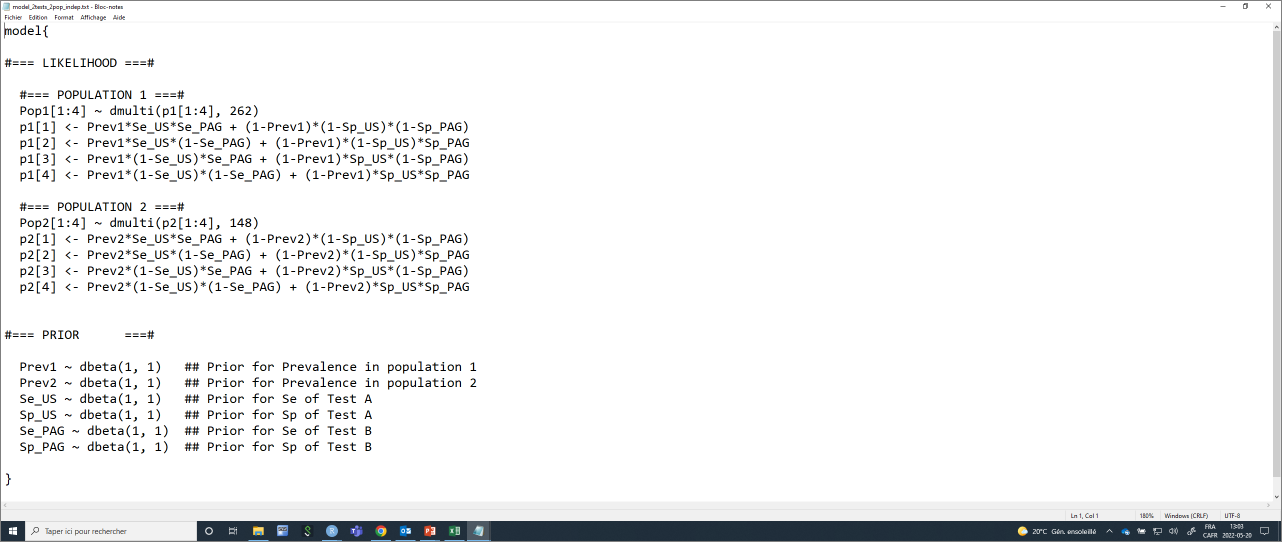
\includegraphics[keepaspectratio]{_main_files/Figures/model_2tests_2pop_indep.png}}
\caption{\textbf{Text file with the model for 2 independent diagnostic tests applied to two populations.}}
\end{figure}

\strut \\
Again, we will need to provide a list of initial values (one per Markov chain) for all unknown parameters. Careful again, we now have two prevalence (\emph{Prev1} and \emph{Prev2}).

\begin{Shaded}
\begin{Highlighting}[]
\CommentTok{\#Initializing values for the parameters Prev, and the Ses and Sps of the two tests for the 3 chains.}
\NormalTok{inits }\OtherTok{\textless{}{-}} \FunctionTok{list}\NormalTok{(}\FunctionTok{list}\NormalTok{(}\AttributeTok{Prev1=}\FloatTok{0.50}\NormalTok{,}
              \AttributeTok{Prev2=}\FloatTok{0.50}\NormalTok{,}
              \AttributeTok{Se\_US=}\FloatTok{0.90}\NormalTok{,}
              \AttributeTok{Sp\_US=}\FloatTok{0.90}\NormalTok{,}
              \AttributeTok{Se\_PAG=}\FloatTok{0.90}\NormalTok{,}
              \AttributeTok{Sp\_PAG=}\FloatTok{0.90}\NormalTok{),}
              
              \FunctionTok{list}\NormalTok{(}\AttributeTok{Prev1=}\FloatTok{0.60}\NormalTok{,}
              \AttributeTok{Prev2=}\FloatTok{0.60}\NormalTok{,}
              \AttributeTok{Se\_US=}\FloatTok{0.80}\NormalTok{,}
              \AttributeTok{Sp\_US=}\FloatTok{0.80}\NormalTok{,}
              \AttributeTok{Se\_PAG=}\FloatTok{0.80}\NormalTok{,}
              \AttributeTok{Sp\_PAG=}\FloatTok{0.80}\NormalTok{),}
              
              \FunctionTok{list}\NormalTok{(}\AttributeTok{Prev1=}\FloatTok{0.40}\NormalTok{,}
              \AttributeTok{Prev2=}\FloatTok{0.40}\NormalTok{,}
              \AttributeTok{Se\_US=}\FloatTok{0.70}\NormalTok{,}
              \AttributeTok{Sp\_US=}\FloatTok{0.70}\NormalTok{,}
              \AttributeTok{Se\_PAG=}\FloatTok{0.70}\NormalTok{,}
              \AttributeTok{Sp\_PAG=}\FloatTok{0.70}\NormalTok{)}
\NormalTok{              )}
\end{Highlighting}
\end{Shaded}

We can run the model using \texttt{jags()} function as seen before.

\begin{Shaded}
\begin{Highlighting}[]
\FunctionTok{library}\NormalTok{(R2jags)}
\FunctionTok{library}\NormalTok{(coda)}

\CommentTok{\#Run the Bayesian model}
\NormalTok{bug.out }\OtherTok{\textless{}{-}} \FunctionTok{jags}\NormalTok{(}\AttributeTok{data=}\NormalTok{datalist,                             }
               \AttributeTok{model.file=}\StringTok{"model\_2tests\_2pop\_indep.txt"}\NormalTok{,     }
               \AttributeTok{parameters.to.save=}\FunctionTok{c}\NormalTok{(}\StringTok{"Prev1"}\NormalTok{, }\StringTok{"Prev2"}\NormalTok{, }\StringTok{"Se\_US"}\NormalTok{, }\StringTok{"Sp\_US"}\NormalTok{, }\StringTok{"Se\_PAG"}\NormalTok{, }\StringTok{"Sp\_PAG"}\NormalTok{),               }
               \AttributeTok{n.chains=}\DecValTok{3}\NormalTok{,                                 }
               \AttributeTok{inits=}\NormalTok{inits,                                }
               \AttributeTok{n.iter=}\DecValTok{11000}\NormalTok{,                                }
               \AttributeTok{n.burnin=}\DecValTok{1000}\NormalTok{,                              }
               \AttributeTok{n.thin=}\DecValTok{1}\NormalTok{,                                   }
               \AttributeTok{DIC=}\ConstantTok{FALSE}\NormalTok{)                                   }
\end{Highlighting}
\end{Shaded}

Then we could produce the diagnostic plots, compute the ESS, and print out our results as we did previously (results not shown).

\begin{Shaded}
\begin{Highlighting}[]
\FunctionTok{library}\NormalTok{(mcmcplots)}
\NormalTok{bug.mcmc }\OtherTok{\textless{}{-}} \FunctionTok{as.mcmc}\NormalTok{(bug.out)          }
\FunctionTok{mcmcplot}\NormalTok{(bug.mcmc, }\AttributeTok{title=}\StringTok{"Diagnostic plots"}\NormalTok{) }
\FunctionTok{effectiveSize}\NormalTok{(bug.mcmc)}
\FunctionTok{print}\NormalTok{(bug.out, }\AttributeTok{digits.summary=}\DecValTok{3}\NormalTok{) }
\end{Highlighting}
\end{Shaded}

\section{Conditional dependence}\label{conditional-dependence}

As discussed before, an important assumption of the LCM described in the previous section is that diagnostic tests are conditionally independent. This assumption, however, can be relaxed using the method proposed by \href{https://onlinelibrary.wiley.com/doi/10.1111/j.0006-341X.2001.00158.x}{Dendukuri and Joseph (2001)}. Note that, we are now increasing the number of unknown parameters and we will, therefore, have to provide additional informative distributions.

\textbf{Table.} Number of degrees of freedom and of unknown parameters when comparing two \textbf{conditionally dependent} diagnostic tests across various number of populations (adapted from \href{https://doi.org/10.20506/rst.40.1.3224}{Cheung et al.~(2021)}).

\begin{longtable}[]{@{}
  >{\centering\arraybackslash}p{(\linewidth - 6\tabcolsep) * \real{0.1753}}
  >{\centering\arraybackslash}p{(\linewidth - 6\tabcolsep) * \real{0.2532}}
  >{\centering\arraybackslash}p{(\linewidth - 6\tabcolsep) * \real{0.2532}}
  >{\centering\arraybackslash}p{(\linewidth - 6\tabcolsep) * \real{0.3182}}@{}}
\toprule\noalign{}
\begin{minipage}[b]{\linewidth}\centering
\textbf{Number of Populations}
\end{minipage} & \begin{minipage}[b]{\linewidth}\centering
\textbf{Number of unknown parameters (np)}
\end{minipage} & \begin{minipage}[b]{\linewidth}\centering
\textbf{Number of degrees of freedom (df)}
\end{minipage} & \begin{minipage}[b]{\linewidth}\centering
\textbf{Minimum number of informative priors needed}
\end{minipage} \\
\midrule\noalign{}
\endhead
\bottomrule\noalign{}
\endlastfoot
1 & 7 & 3 & 4 \\
2 & 8 & 6 & 2 \\
3 & 9 & 9 & 0 \\
4 & 10 & 12 & 0 \\
p & 4+2+p & 3*p & if df \textless{} np, then np-df \\
\end{longtable}

For this example, in addition to specifying priors for \emph{covp} and \emph{covn}, we will add informative priors on US \emph{Se} and \emph{Sp}.

\begin{Shaded}
\begin{Highlighting}[]
\FunctionTok{library}\NormalTok{(epiR)}
\CommentTok{\# US sensitivity {-}{-}{-}{-}{-}{-}{-}{-}{-}{-}{-}{-}{-}{-}{-}{-}{-}{-}{-}{-}{-}{-}{-}{-}{-}{-}{-}{-}{-}{-}{-}{-}{-}{-}{-}{-}{-}{-}{-}{-}{-}{-}{-}{-}{-}{-}{-}{-}{-}{-}{-}{-}{-}{-}{-}{-}{-}{-}}
\CommentTok{\# Sensitivity of US:  Mode=0.90, and we are 97.5\% sure \textgreater{}0.85 }
\NormalTok{Se.US }\OtherTok{\textless{}{-}} \FunctionTok{epi.betabuster}\NormalTok{(}\AttributeTok{mode=}\FloatTok{0.90}\NormalTok{, }\AttributeTok{conf=}\FloatTok{0.975}\NormalTok{, }\AttributeTok{imsure=}\StringTok{"greater than"}\NormalTok{, }\AttributeTok{x=}\FloatTok{0.85}\NormalTok{)  }

\CommentTok{\# US specificity {-}{-}{-}{-}{-}{-}{-}{-}{-}{-}{-}{-}{-}{-}{-}{-}{-}{-}{-}{-}{-}{-}{-}{-}{-}{-}{-}{-}{-}{-}{-}{-}{-}{-}{-}{-}{-}{-}{-}{-}{-}{-}{-}{-}{-}{-}{-}{-}{-}{-}{-}{-}{-}{-}{-}{-}{-}{-}}
\CommentTok{\# Specificity of US:  Mode=0.95, and we are 97.5\% sure \textgreater{}0.90 }
\NormalTok{Sp.US }\OtherTok{\textless{}{-}} \FunctionTok{epi.betabuster}\NormalTok{(}\AttributeTok{mode=}\FloatTok{0.95}\NormalTok{, }\AttributeTok{conf=}\FloatTok{0.975}\NormalTok{, }\AttributeTok{imsure=}\StringTok{"greater than"}\NormalTok{, }\AttributeTok{x=}\FloatTok{0.90}\NormalTok{)  }

\NormalTok{Se.TestA.shapea }\OtherTok{\textless{}{-}}\NormalTok{ Se.US}\SpecialCharTok{$}\NormalTok{shape1     }\CommentTok{\#a shape parameter for Se of TestA}
\NormalTok{Se.TestA.shapeb }\OtherTok{\textless{}{-}}\NormalTok{ Se.US}\SpecialCharTok{$}\NormalTok{shape2     }\CommentTok{\#b shape parameter for Se of TestA}
\NormalTok{Sp.TestA.shapea }\OtherTok{\textless{}{-}}\NormalTok{ Sp.US}\SpecialCharTok{$}\NormalTok{shape1     }\CommentTok{\#a shape parameter for Sp of TestA}
\NormalTok{Sp.TestA.shapeb }\OtherTok{\textless{}{-}}\NormalTok{ Sp.US}\SpecialCharTok{$}\NormalTok{shape2     }\CommentTok{\#b shape parameter for Sp of TestA}
\end{Highlighting}
\end{Shaded}

Now, we could add the \emph{covp} and \emph{covn} parameters in the likelihood function, and specified prior distributions for these as we did before:

\begin{Shaded}
\begin{Highlighting}[]
\CommentTok{\#Create the JAGS text file}
\NormalTok{model\_2tests\_2pop\_dep }\OtherTok{\textless{}{-}} \FunctionTok{paste0}\NormalTok{(}\StringTok{"model\{}

\StringTok{\#=== LIKELIHOOD ===\#}

\StringTok{  \#=== POPULATION 1 ===\#}
\StringTok{  Pop1[1:4] \textasciitilde{} dmulti(p1[1:4], "}\NormalTok{,nPop1,}\StringTok{")}
\StringTok{  p1[1] \textless{}{-} Prev1*(Se\_"}\NormalTok{, TestA, }\StringTok{"*Se\_"}\NormalTok{, TestB, }\StringTok{" + covp) + (1{-}Prev1)*((1{-}Sp\_"}\NormalTok{, TestA, }\StringTok{")*(1{-}Sp\_"}\NormalTok{, TestB, }\StringTok{") + covn)}
\StringTok{  p1[2] \textless{}{-} Prev1*(Se\_"}\NormalTok{, TestA, }\StringTok{"*(1{-}Se\_"}\NormalTok{, TestB, }\StringTok{") {-} covp) + (1{-}Prev1)*((1{-}Sp\_"}\NormalTok{, TestA, }\StringTok{")*Sp\_"}\NormalTok{, TestB, }\StringTok{" {-} covn)}
\StringTok{  p1[3] \textless{}{-} Prev1*((1{-}Se\_"}\NormalTok{, TestA, }\StringTok{")*Se\_"}\NormalTok{, TestB, }\StringTok{" {-} covp) + (1{-}Prev1)*(Sp\_"}\NormalTok{, TestA, }\StringTok{"*(1{-}Sp\_"}\NormalTok{, TestB, }\StringTok{") {-} covn)}
\StringTok{  p1[4] \textless{}{-} Prev1*((1{-}Se\_"}\NormalTok{, TestA, }\StringTok{")*(1{-}Se\_"}\NormalTok{, TestB, }\StringTok{") + covp) + (1{-}Prev1)*(Sp\_"}\NormalTok{, TestA, }\StringTok{"*Sp\_"}\NormalTok{, TestB, }\StringTok{" + covn)}

\StringTok{  \#=== POPULATION 2 ===\#  }
\StringTok{  Pop2[1:4] \textasciitilde{} dmulti(p2[1:4], "}\NormalTok{,nPop2,}\StringTok{")}
\StringTok{  p2[1] \textless{}{-} Prev2*(Se\_"}\NormalTok{, TestA, }\StringTok{"*Se\_"}\NormalTok{, TestB, }\StringTok{" + covp) + (1{-}Prev2)*((1{-}Sp\_"}\NormalTok{, TestA, }\StringTok{")*(1{-}Sp\_"}\NormalTok{, TestB, }\StringTok{") + covn)}
\StringTok{  p2[2] \textless{}{-} Prev2*(Se\_"}\NormalTok{, TestA, }\StringTok{"*(1{-}Se\_"}\NormalTok{, TestB, }\StringTok{") {-} covp) + (1{-}Prev2)*((1{-}Sp\_"}\NormalTok{, TestA, }\StringTok{")*Sp\_"}\NormalTok{, TestB, }\StringTok{" {-} covn)}
\StringTok{  p2[3] \textless{}{-} Prev2*((1{-}Se\_"}\NormalTok{, TestA, }\StringTok{")*Se\_"}\NormalTok{, TestB, }\StringTok{" {-} covp) + (1{-}Prev2)*(Sp\_"}\NormalTok{, TestA, }\StringTok{"*(1{-}Sp\_"}\NormalTok{, TestB, }\StringTok{") {-} covn)}
\StringTok{  p2[4] \textless{}{-} Prev2*((1{-}Se\_"}\NormalTok{, TestA, }\StringTok{")*(1{-}Se\_"}\NormalTok{, TestB, }\StringTok{") + covp) + (1{-}Prev2)*(Sp\_"}\NormalTok{, TestA, }\StringTok{"*Sp\_"}\NormalTok{, TestB, }\StringTok{" + covn)}

\StringTok{  }
\StringTok{  }
\StringTok{\#=== PRIOR  ===\#}

\StringTok{  Prev1 \textasciitilde{} dbeta("}\NormalTok{,Prev1.shapea,}\StringTok{", "}\NormalTok{,Prev1.shapeb,}\StringTok{")     \#\# Prior for Prevalence in population 1}
\StringTok{  Prev2 \textasciitilde{} dbeta("}\NormalTok{,Prev2.shapea,}\StringTok{", "}\NormalTok{,Prev2.shapeb,}\StringTok{")     \#\# Prior for Prevalence in population 2}
\StringTok{  Se\_"}\NormalTok{, TestA, }\StringTok{" \textasciitilde{} dbeta("}\NormalTok{,Se.TestA.shapea,}\StringTok{", "}\NormalTok{,Se.TestA.shapeb,}\StringTok{")  \#\# Prior for Se of Test A}
\StringTok{  Sp\_"}\NormalTok{, TestA, }\StringTok{" \textasciitilde{} dbeta("}\NormalTok{,Sp.TestA.shapea,}\StringTok{", "}\NormalTok{,Sp.TestA.shapeb,}\StringTok{")  \#\# Prior for Sp of Test A}
\StringTok{  Se\_"}\NormalTok{, TestB, }\StringTok{" \textasciitilde{} dbeta("}\NormalTok{,Se.TestB.shapea,}\StringTok{", "}\NormalTok{,Se.TestB.shapeb,}\StringTok{")  \#\# Prior for Se of Test B}
\StringTok{  Sp\_"}\NormalTok{, TestB, }\StringTok{" \textasciitilde{} dbeta("}\NormalTok{,Sp.TestB.shapea,}\StringTok{", "}\NormalTok{,Sp.TestB.shapeb,}\StringTok{")  \#\# Prior for Sp of Test B}
\StringTok{  }
\StringTok{  \#=== CONDITIONAL DEPENDENCE STRUCTURE ===\#}

\StringTok{  covp \textasciitilde{} dunif(minp,maxp)}
\StringTok{  covn \textasciitilde{} dunif(minn,maxn)}
\StringTok{  minp \textless{}{-} (1{-}Se\_"}\NormalTok{, TestA, }\StringTok{")*(Se\_"}\NormalTok{, TestB, }\StringTok{"{-}1)}
\StringTok{  minn \textless{}{-} (Sp\_"}\NormalTok{, TestA, }\StringTok{"{-}1)*(1{-}Sp\_"}\NormalTok{, TestB, }\StringTok{")}
\StringTok{  maxp \textless{}{-} min(Se\_"}\NormalTok{, TestA, }\StringTok{",Se\_"}\NormalTok{, TestB, }\StringTok{") {-} Se\_"}\NormalTok{, TestA, }\StringTok{"*Se\_"}\NormalTok{, TestB, }\StringTok{"    }
\StringTok{  maxn \textless{}{-} min(Sp\_"}\NormalTok{, TestA, }\StringTok{",Sp\_"}\NormalTok{, TestB, }\StringTok{") {-} Sp\_"}\NormalTok{, TestA, }\StringTok{"*Sp\_"}\NormalTok{, TestB, }\StringTok{"  }
\StringTok{  }
\StringTok{\}"}\NormalTok{)}

\CommentTok{\#write as a text (.txt) file}
\FunctionTok{write.table}\NormalTok{(model\_2tests\_2pop\_dep, }
            \AttributeTok{file=}\StringTok{"model\_2tests\_2pop\_dep.txt"}\NormalTok{, }
            \AttributeTok{quote=}\ConstantTok{FALSE}\NormalTok{, }
            \AttributeTok{sep=}\StringTok{""}\NormalTok{, }
            \AttributeTok{row.names=}\ConstantTok{FALSE}\NormalTok{,}
            \AttributeTok{col.names=}\ConstantTok{FALSE}\NormalTok{)}
\end{Highlighting}
\end{Shaded}

This text file looks like this:

\begin{figure}
\centering
\pandocbounded{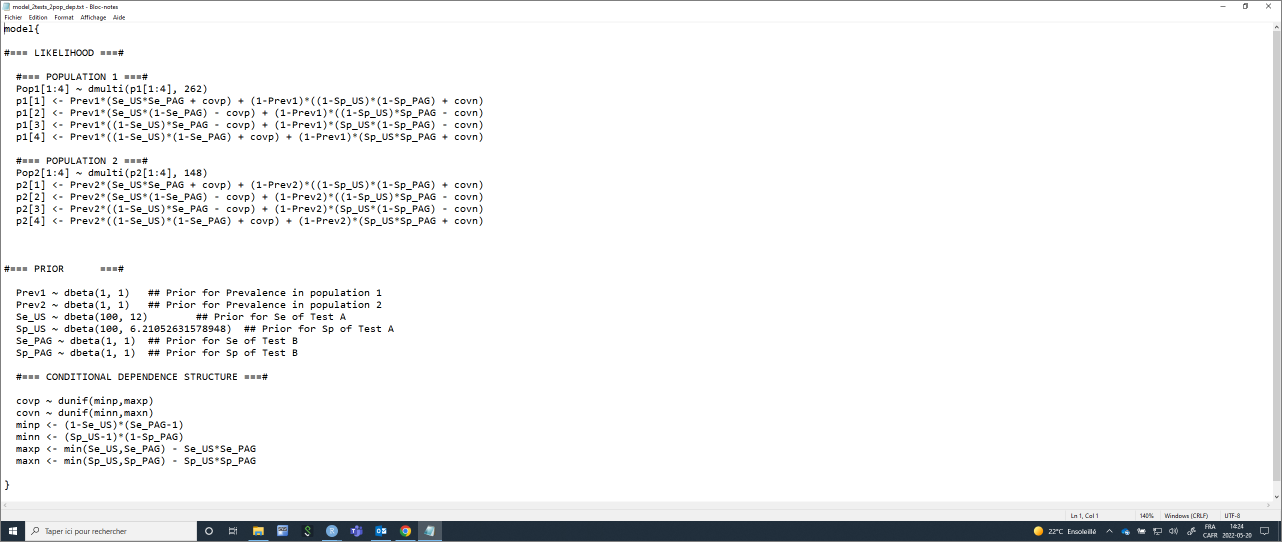
\includegraphics[keepaspectratio]{_main_files/Figures/model_2tests_2pop_dep.png}}
\caption{\textbf{Text file with the model for 2 DEPENDENT diagnostic tests applied to two populations.}}
\end{figure}

\strut \\
Again, the list of initial values will have to be modified to include (\emph{covp} and \emph{covn}).

\begin{Shaded}
\begin{Highlighting}[]
\CommentTok{\#Initializing values for the parameters Prev, and the Ses and Sps of the two tests for the 3 chains.}
\NormalTok{inits }\OtherTok{\textless{}{-}} \FunctionTok{list}\NormalTok{(}\FunctionTok{list}\NormalTok{(}\AttributeTok{Prev1=}\FloatTok{0.50}\NormalTok{,}
              \AttributeTok{Prev2=}\FloatTok{0.50}\NormalTok{,}
              \AttributeTok{Se\_US=}\FloatTok{0.90}\NormalTok{,}
              \AttributeTok{Sp\_US=}\FloatTok{0.90}\NormalTok{,}
              \AttributeTok{Se\_PAG=}\FloatTok{0.90}\NormalTok{,}
              \AttributeTok{Sp\_PAG=}\FloatTok{0.90}\NormalTok{,}
              \AttributeTok{covp=}\FloatTok{0.0}\NormalTok{,}
              \AttributeTok{covn=}\FloatTok{0.0}\NormalTok{),}
              
              \FunctionTok{list}\NormalTok{(}\AttributeTok{Prev1=}\FloatTok{0.60}\NormalTok{,}
              \AttributeTok{Prev2=}\FloatTok{0.60}\NormalTok{,}
              \AttributeTok{Se\_US=}\FloatTok{0.80}\NormalTok{,}
              \AttributeTok{Sp\_US=}\FloatTok{0.80}\NormalTok{,}
              \AttributeTok{Se\_PAG=}\FloatTok{0.80}\NormalTok{,}
              \AttributeTok{Sp\_PAG=}\FloatTok{0.80}\NormalTok{,}
              \AttributeTok{covp=}\FloatTok{0.01}\NormalTok{,}
              \AttributeTok{covn=}\FloatTok{0.01}\NormalTok{),}
              
              \FunctionTok{list}\NormalTok{(}\AttributeTok{Prev1=}\FloatTok{0.40}\NormalTok{,}
              \AttributeTok{Prev2=}\FloatTok{0.40}\NormalTok{,}
              \AttributeTok{Se\_US=}\FloatTok{0.70}\NormalTok{,}
              \AttributeTok{Sp\_US=}\FloatTok{0.70}\NormalTok{,}
              \AttributeTok{Se\_PAG=}\FloatTok{0.70}\NormalTok{,}
              \AttributeTok{Sp\_PAG=}\FloatTok{0.70}\NormalTok{,}
              \AttributeTok{covp=}\FloatTok{0.05}\NormalTok{,}
              \AttributeTok{covn=}\FloatTok{0.05}\NormalTok{)}
\NormalTok{              )}
\end{Highlighting}
\end{Shaded}

And, when running the model using \texttt{jags()}, we would also ask to monitor \emph{covp} and \emph{covn}. Note that we have increased the number of iterations / burn-in period (remember the autocorrelation problem seen with LCM with a covariance between tests?).

\begin{Shaded}
\begin{Highlighting}[]
\FunctionTok{library}\NormalTok{(R2jags)}
\FunctionTok{library}\NormalTok{(coda)}

\CommentTok{\#Run the Bayesian model}
\NormalTok{bug.out }\OtherTok{\textless{}{-}} \FunctionTok{jags}\NormalTok{(}\AttributeTok{data=}\NormalTok{datalist,                             }
               \AttributeTok{model.file=}\StringTok{"model\_2tests\_2pop\_dep.txt"}\NormalTok{,     }
               \AttributeTok{parameters.to.save=}\FunctionTok{c}\NormalTok{(}\StringTok{"Prev1"}\NormalTok{, }\StringTok{"Prev2"}\NormalTok{, }\StringTok{"Se\_US"}\NormalTok{, }\StringTok{"Sp\_US"}\NormalTok{, }\StringTok{"Se\_PAG"}\NormalTok{, }\StringTok{"Sp\_PAG"}\NormalTok{, }\StringTok{"covp"}\NormalTok{, }\StringTok{"covn"}\NormalTok{),               }
               \AttributeTok{n.chains=}\DecValTok{3}\NormalTok{,                                 }
               \AttributeTok{inits=}\NormalTok{inits,                                }
               \AttributeTok{n.iter=}\DecValTok{210000}\NormalTok{,                                }
               \AttributeTok{n.burnin=}\DecValTok{10000}\NormalTok{,                              }
               \AttributeTok{n.thin=}\DecValTok{1}\NormalTok{,                                   }
               \AttributeTok{DIC=}\ConstantTok{FALSE}\NormalTok{)                                   }
\end{Highlighting}
\end{Shaded}

\begin{verbatim}
## Compiling model graph
##    Resolving undeclared variables
##    Allocating nodes
## Graph information:
##    Observed stochastic nodes: 2
##    Unobserved stochastic nodes: 8
##    Total graph size: 72
## 
## Initializing model
\end{verbatim}

Then we could produce the diagnostic plots, compute the ESS, and print out our results as we did previously (results not shown).

\begin{Shaded}
\begin{Highlighting}[]
\FunctionTok{library}\NormalTok{(mcmcplots)}
\NormalTok{bug.mcmc }\OtherTok{\textless{}{-}} \FunctionTok{as.mcmc}\NormalTok{(bug.out)          }
\FunctionTok{mcmcplot}\NormalTok{(bug.mcmc, }\AttributeTok{title=}\StringTok{"Diagnostic plots"}\NormalTok{) }
\FunctionTok{effectiveSize}\NormalTok{(bug.mcmc)}
\FunctionTok{print}\NormalTok{(bug.out, }\AttributeTok{digits.summary=}\DecValTok{3}\NormalTok{) }
\end{Highlighting}
\end{Shaded}

\section{Hierarchical latent class models}\label{hierarchical-latent-class-models}

\subsection{The general idea}\label{the-general-idea}

In a given study, you may have measured individuals from a substantial number of sub-populations. For instance, in the \href{https://www.sciencedirect.com/science/article/pii/S016758771630527X?via\%3Dihub}{Dufour et al.~(2017)} original study comparing the PAG-ELISA and ultrasound tests for diagnosing pregnancy in dairy cows, cows from 18 commercial dairy herds were studied. In such case, we could, for instance, split the data in 18 sub-populations and use the models described in the preceding sections, with 18 likelihood functions, and where we would estimate 18 prevalence (one for each herd). This approach is totally fine, but it may not be the most elegant, nor efficient model for that type of study. If we were to use this approach, and assuming conditional independence between tests, we would have:

\begin{itemize}
\tightlist
\item
  22 unknown parameters to estimate (\emph{SeA} and \emph{SpA}, \emph{SeB} and \emph{SpB}, and each sub-population's prevalence, \emph{P1} to \emph{P18} in this case);\\
\item
  54 degrees of freedom (3 degrees of freedom for each 2x2 table, and 18 2x2 tables).
\end{itemize}

Nevertheless, this would be an identifiable model and we would not necessarily require informative priors.

On the other hand, \href{https://link.springer.com/article/10.1198/1085711031526}{Hanson et al.~(2003)} have proposed a slightly different, and possibly more elegant and efficient, modelling approach named the hierarchical latent class model. Actually, in most cases, \textbf{estimating the disease prevalence in each of the sub-populations (e.g., in each of the 18 herds in the PAG study) is not a primary objective as compared to estimating} test accuracy and/or \textbf{the distribution of within-herd prevalence in the population of herds from which these herds were sampled (i.e., the source population)}. In such case, we could use the model described in the figure below.

\begin{figure}
\centering
\pandocbounded{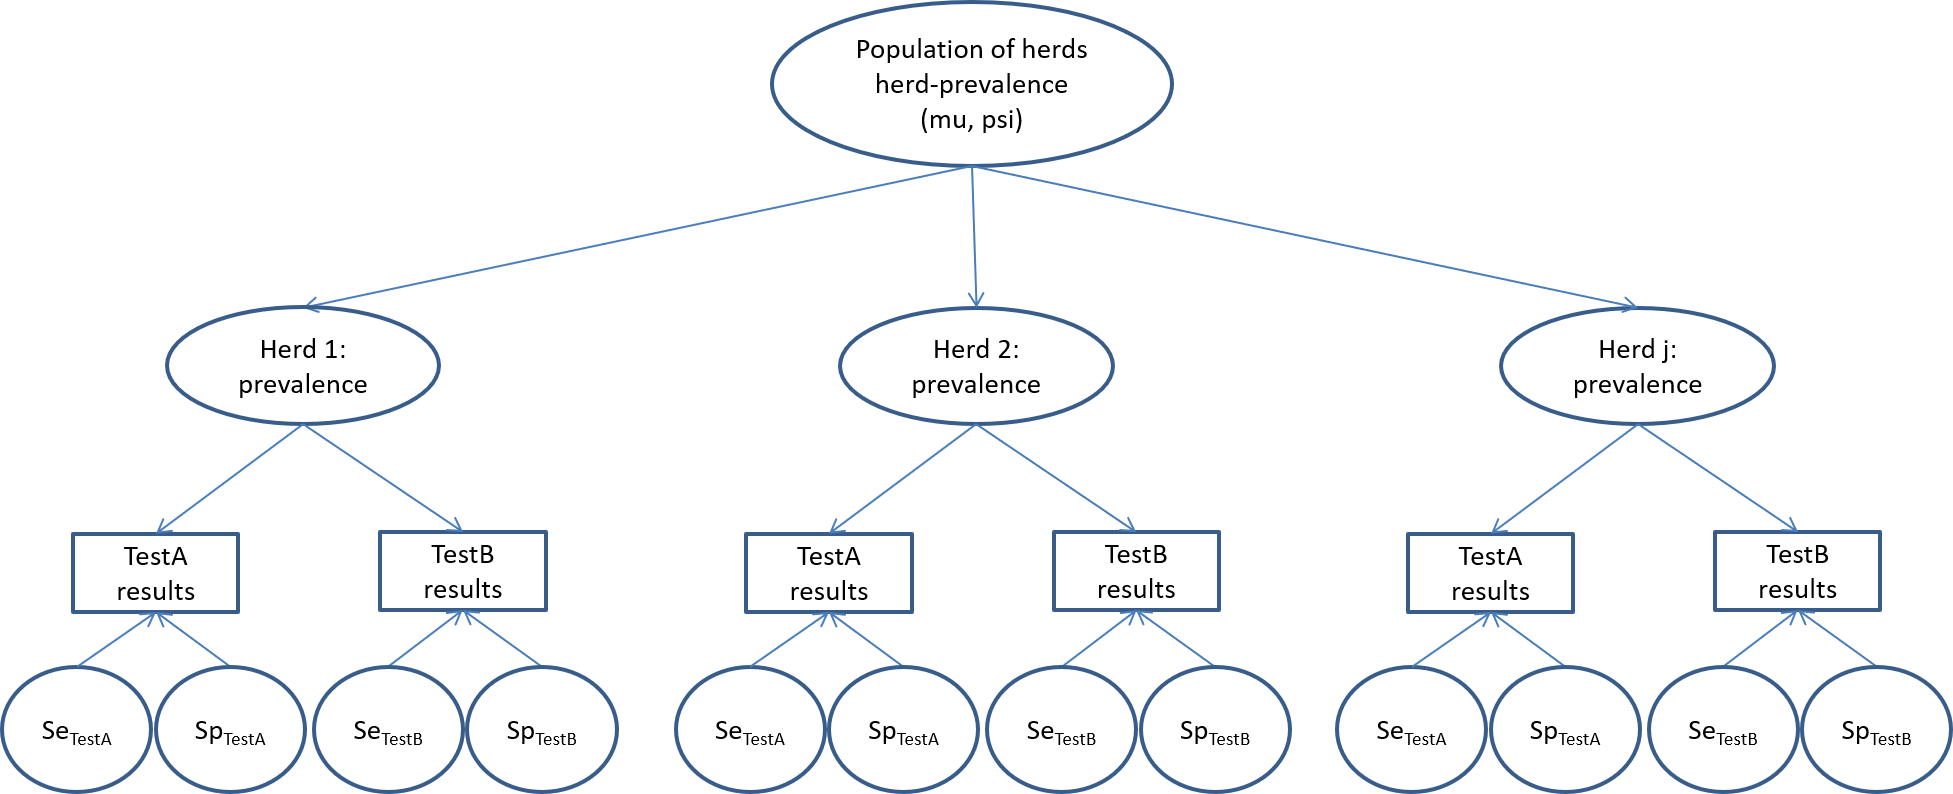
\includegraphics[keepaspectratio]{_main_files/Figures/Hierarchical model.png}}
\caption{\textbf{Diagrammatic representation of Hanson et al.~(2005) hierarchical latent class model. Rectangles represent observed variables (results of the two tests), ovals represent latent variable (individual herd's disease prevalence and population's distribution of within-herd prevalence), and circles represent the unknown accuracy parameters (Se and Sp of the two tests).}}
\end{figure}

\strut \\
Briefly, in this model we would assume that each of the recruited herds originated from a large population of herds (the source population). We would then only need to describe the distribution of within-herd prevalence of the source population (rather than the prevalence of sick individuals of each herd, as we did so far). We could propose a \emph{beta(a, b)} distribution as prior for this distribution of within-herd prevalence. Given the hierarchical nature of the priors (i.e., the priors are on the source population, not on the studied sub-populations), we will rather refer to them as \textbf{hyperpriors}. In the hierarchical model, instead of providing hyperpriors for \emph{a} and \emph{b}, we will instead provide hyperpriors for \emph{mu} and \emph{psi}. Remember from Chapter 2 that:

\begin{itemize}
\tightlist
\item
  \emph{mu} represents how the mean within-herd prevalence varies in the source population of herds;\\
\item
  \emph{psi} describes the spread of the distribution around the mean within-herd prevalence in the source population of herds.
\end{itemize}

And also, in a \emph{beta(a,b)} distribution:

\(a = mu*psi\)\\
\(b = psi*(1-mu)\)

For \emph{mu}, it would be quite natural to use a beta distribution as hyperprior, given that the mean within-herd prevalence need to be bounded by 0.0 and 1.0. For \emph{psi}, which represent a variance, a gamma distribution would be a better option for this hyperprior.

We have not discussed gamma distributions in Chapter 2, since they are not used in the other BLCM presented in this document. Briefly, the gamma distribution is also defined by two parameters \emph{α} and \emph{β}. The \emph{α} parameter is also known as the \emph{shape} parameter and the \emph{β} parameter is known as the \emph{rate} parameter. Gamma distributions can take different forms, but are bounded to values between 0 and ∞. Moreover, a \textbf{Gamma(0.001, 0.001) would correspond to a vague gamma distribution.}

\subsection{The likelihood function}\label{the-likelihood-function-1}

We could described the likelihood function for the hierarchical model as follow:

\(\text{for i in  }1:NumberOfHerds\)\\
\(n[i,1:4] \sim dmulti(p[i,1:4], NumAnimInHerd[i])\)

\(p[i,1] = prevInHerd[i]*SeA*SeB + (1-prevInHerd[i])*(1-SpA)*(1-SpB)\)\\
\(p[i,2] = prevInHerd[i]*SeA*(1-SeB) + (1-prevInHerd[i])*(1-SpA)*SpB\)\\
\(p[i,3] = prevInHerd[i]*(1-SeA)*SeB + (1-prevInHerd[i])*SpA*(1-SpB)\)\\
\(p[i,4] = prevInHerd[i]*(1-SeA)*(1-SeB) + (1-prevInHerd[i])*SpA*SpB\)

\(prevInHerd[i] \sim dbeta(alpha, beta)\)\\
\(alpha = mu*psi\)\\
\(beta = psi*(1-mu)\)

Where \emph{NumberOfHerds} is the number of sub-populations in the study, \emph{n{[}i,1:4{]}} is the content, for each sub-population, of the 4 cells (\emph{n1}, \emph{n2}, \emph{n3}, and \emph{n4}) from the 2x2 tables with cross-classified tests results (i.e., the observed data), \emph{NumAnimInHerd{[}i{]}} is the number of individuals tested in each sub-population, and \emph{prevInHerd{[}i{]}} is the prevalence of disease in each sub-population. \emph{dbeta(alpha, beta)} is the distribution of within-herd prevalence in the source population (assumed to follow a beta distribution) and is defined by two unknown parameters, \emph{mu} and \emph{psi}, for which we will have to propose hyperpriors. We could use a beta hyperprior for \emph{mu} and a gamma hyperprior for \emph{psi}. These hyperpriors could be vague (e.g., beta(1.0, 1.0) and gamma(0.001, 0.001)) or informative (we will see in a following section how to propose informative hyperpriors for \emph{mu} and \emph{psi}).

If we examine the hierarchical model more carefully, we see one important difference between this model and the models we have used so far, the inclusion of a loop in the likelihood function. Briefly, we are asking to repeat this likelihood function for each sub-population (i.e., \emph{for (i in 1:NumberOfHerds)}). Again, if we try to translate this likelihood function in words, and focusing on Herd \#1 (to simplify) the number of individuals in cell \emph{n1} (i.e., TestA+ and TestB+) is determined by the number of individuals tested in Herd \#1 (\emph{NumAnimInHerd{[}1{]}}) and the probability (\emph{p{[}1{]}}) of falling in that cell. The latter itself depends on the true prevalence of disease in Herd \#1 (\emph{prevInHerd{[}1{]}}; which can be drawn from the source population distribution of within-herd prevalence, \emph{dbeta(alpha, beta)}), and on each of the two tests sensitivity (\emph{SeA} and \emph{SeB}) and specificity (\emph{SpA} and \emph{SpB}). We can use similar reasoning for \emph{n2}, \emph{n3}, and \emph{n4}. Finally, the multinomial distribution would further impose that the four probabilities (\emph{p{[}1{]}}, \emph{p{[}2{]}}, \emph{p{[}3{]}}, and \emph{p{[}4{]}}) have to sum up to 1.0 (i.e., 100\%) within a given herd.

Note that we now have:

\begin{itemize}
\tightlist
\item
  6 unknown parameters to estimate (\emph{SeA} and \emph{SpA}, \emph{SeB} and \emph{SpB}, \emph{mu}, and \emph{psi}), as compared to 4 parameters plus one parameter for each sub-population for the approach described in the preceding sections;\\
\item
  3 degrees of freedom for each sub-population.
\end{itemize}

For instance, with the 18 commercial herds available in the \href{https://www.sciencedirect.com/science/article/pii/S016758771630527X?via\%3Dihub}{Dufour et al.~(2017)} original study, we would have 6 unknown parameters and 54 degrees of freedom. If we were to use 30 herds, we would still have 6 unknown parameters, but now 90 degrees of freedom, etc. This is the reason why we described the \href{https://link.springer.com/article/10.1198/1085711031526}{Hanson et al.~(2003)} hierarchical model as ``more efficient''.

\subsection{The data}\label{the-data-1}

Data for the hierarchical model will have to be organized as follow. Briefly, we will first need a \textbf{dataset where we report, for each sub-population, the number of individuals with a given combination of tests results}. For instance, below we are importing an Excel sheet with the organized results. The example below is reproduced from \href{https://www.sciencedirect.com/science/article/pii/S016758771630527X?via\%3Dihub}{Dufour et al.~(2017; Table 1)}.

\begin{Shaded}
\begin{Highlighting}[]
\FunctionTok{library}\NormalTok{(readxl)   }\CommentTok{\#A library that can import .xlsx documents }
\NormalTok{obs }\OtherTok{\textless{}{-}} \FunctionTok{read\_excel}\NormalTok{(}\StringTok{"Data/Herd level results.xlsx"}\NormalTok{)}
\CommentTok{\#Check the data}
\NormalTok{obs}
\end{Highlighting}
\end{Shaded}

\begin{verbatim}
## # A tibble: 18 x 4
##    `TestA+TestB+` `TestA+TestB-` `TestA-TestB+` `TestA-TestB-`
##             <dbl>          <dbl>          <dbl>          <dbl>
##  1             20              0              2             14
##  2              7              0              0              4
##  3             10              0              0             10
##  4             12              0              1             21
##  5             17              0              2              9
##  6              2              0              0              3
##  7             46              1              3             37
##  8              0              0              0              1
##  9              7              0              1              5
## 10              7              0              0              3
## 11             12              1              2             12
## 12              8              0              1              7
## 13             11              0              0              9
## 14              5              0              1             10
## 15             71              0              8             69
## 16             10              0              0              3
## 17              5              0              0              1
## 18              5              0              0              1
\end{verbatim}

You can see that we have used this order:

\begin{itemize}
\tightlist
\item
  \emph{TestA} + and \emph{TestB} +\\
\item
  \emph{TestA} + and \emph{TestB} -\\
\item
  \emph{TestA} - and \emph{TestB} +\\
\item
  \emph{TestA} - and \emph{TestB} -
\end{itemize}

This will be important, because we will use the same order for the 4 probabilities in the likelihood function.

Then, we will need a \textbf{second dataset where we report the total number of individual tested by sub-population}. This can be computed from the above dataset as follow:

\begin{Shaded}
\begin{Highlighting}[]
\CommentTok{\#Compute total number of animals by herd}
\NormalTok{totals }\OtherTok{\textless{}{-}} \FunctionTok{rowSums}\NormalTok{(obs)}
\CommentTok{\#Check the total number of animals per herd}
\NormalTok{totals}
\end{Highlighting}
\end{Shaded}

\begin{verbatim}
##  [1]  36  11  20  34  28   5  87   1  13  10  27  16  20  16 148  13   6   6
\end{verbatim}

The previous two pieces of data will have to be reunited together. We can do this using:

\begin{Shaded}
\begin{Highlighting}[]
\NormalTok{datalist }\OtherTok{\textless{}{-}} \FunctionTok{list}\NormalTok{(}\AttributeTok{obs=}\NormalTok{obs, }\AttributeTok{totals=}\NormalTok{totals)}
\CommentTok{\#Check the datalist}
\NormalTok{datalist}
\end{Highlighting}
\end{Shaded}

\begin{verbatim}
## $obs
## # A tibble: 18 x 4
##    `TestA+TestB+` `TestA+TestB-` `TestA-TestB+` `TestA-TestB-`
##             <dbl>          <dbl>          <dbl>          <dbl>
##  1             20              0              2             14
##  2              7              0              0              4
##  3             10              0              0             10
##  4             12              0              1             21
##  5             17              0              2              9
##  6              2              0              0              3
##  7             46              1              3             37
##  8              0              0              0              1
##  9              7              0              1              5
## 10              7              0              0              3
## 11             12              1              2             12
## 12              8              0              1              7
## 13             11              0              0              9
## 14              5              0              1             10
## 15             71              0              8             69
## 16             10              0              0              3
## 17              5              0              0              1
## 18              5              0              0              1
## 
## $totals
##  [1]  36  11  20  34  28   5  87   1  13  10  27  16  20  16 148  13   6   6
\end{verbatim}

Finally, we will need to know the \textbf{number of sub-populations studied}. Again, this can be computed as follow:

\begin{Shaded}
\begin{Highlighting}[]
\CommentTok{\#Compute number of herds}
\NormalTok{numherd }\OtherTok{\textless{}{-}} \FunctionTok{dim}\NormalTok{(obs)[}\DecValTok{1}\NormalTok{]}
\CommentTok{\#Check number of herd}
\NormalTok{numherd}
\end{Highlighting}
\end{Shaded}

\begin{verbatim}
## [1] 18
\end{verbatim}

We could also assign labels to the tests for future usage, as we did before:

\begin{Shaded}
\begin{Highlighting}[]
\NormalTok{TestA }\OtherTok{\textless{}{-}} \StringTok{"US"}
\NormalTok{TestB }\OtherTok{\textless{}{-}} \StringTok{"PAG"}
\end{Highlighting}
\end{Shaded}

\subsection{The priors}\label{the-priors}

We will need to assign priors (or hyperpriors) for \emph{mu}, \emph{psi}, \emph{SeA} and \emph{SpA}, \emph{SeB} and \emph{SpB}. Below, we have used vague priors (or hyperpriors) for all these unknown parameters. If we were to use informative priors for \emph{SeA}, \emph{SpA}, \emph{SeB}, or \emph{SpB}, we could implement this as in the previous chapters. Informative priors for \emph{mu} and \emph{psi} are bit more tedious to generate; we will describe in a following section how to achieve this.

\begin{Shaded}
\begin{Highlighting}[]
\NormalTok{mu.shapea }\OtherTok{\textless{}{-}} \FloatTok{1.0}           \CommentTok{\# a shape parameter for mu}
\NormalTok{mu.shapeb }\OtherTok{\textless{}{-}} \FloatTok{1.0}           \CommentTok{\# b shape parameter for mu}

\NormalTok{psi.shapea }\OtherTok{\textless{}{-}} \FloatTok{0.001}        \CommentTok{\# α (shape) parameter for gamma}
\NormalTok{psi.shapeb }\OtherTok{\textless{}{-}} \FloatTok{0.001}        \CommentTok{\# β (rate) parameter for gamma}

\NormalTok{Se.TestA.shapea }\OtherTok{\textless{}{-}} \DecValTok{1}       \CommentTok{\#a shape parameter for Se of TestA}
\NormalTok{Se.TestA.shapeb }\OtherTok{\textless{}{-}} \DecValTok{1}       \CommentTok{\#b shape parameter for Se of TestA}
\NormalTok{Sp.TestA.shapea }\OtherTok{\textless{}{-}} \DecValTok{1}       \CommentTok{\#a shape parameter for Sp of TestA}
\NormalTok{Sp.TestA.shapeb }\OtherTok{\textless{}{-}} \DecValTok{1}       \CommentTok{\#b shape parameter for Sp of TestA}

\NormalTok{Se.TestB.shapea }\OtherTok{\textless{}{-}} \DecValTok{1}       \CommentTok{\#a shape parameter for Se of TestB}
\NormalTok{Se.TestB.shapeb }\OtherTok{\textless{}{-}} \DecValTok{1}       \CommentTok{\#b shape parameter for Se of TestB}
\NormalTok{Sp.TestB.shapea }\OtherTok{\textless{}{-}} \DecValTok{1}       \CommentTok{\#a shape parameter for Sp of TestB}
\NormalTok{Sp.TestB.shapeb }\OtherTok{\textless{}{-}} \DecValTok{1}       \CommentTok{\#b shape parameter for Sp of TestB}
\end{Highlighting}
\end{Shaded}

\subsection{Write the JAGS model}\label{write-the-jags-model}

The text file we would like to generate would look as the screen capture below.

\begin{figure}
\centering
\pandocbounded{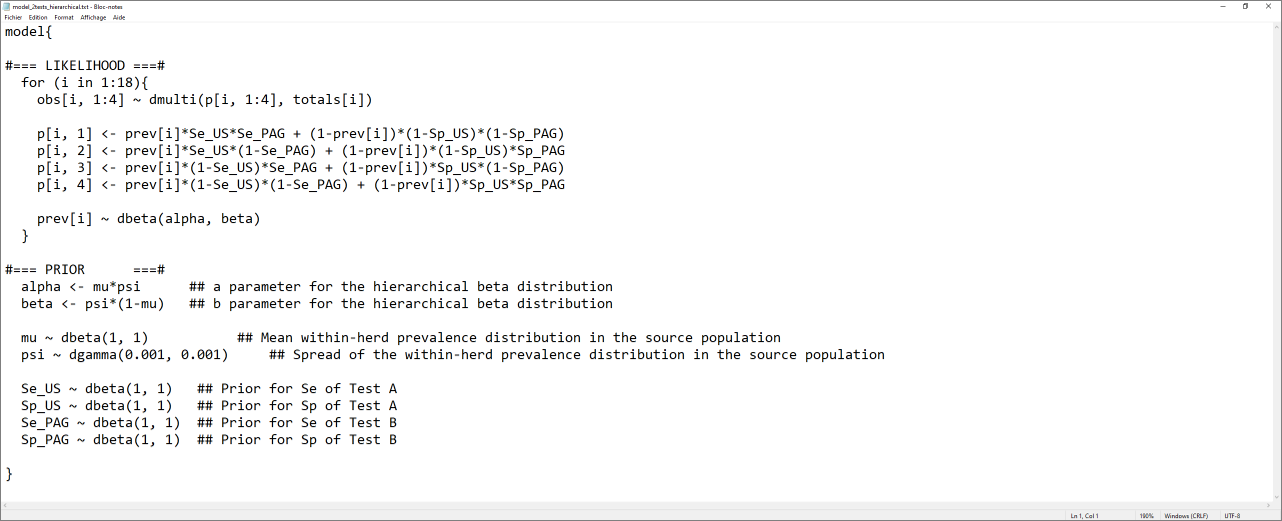
\includegraphics[keepaspectratio]{_main_files/Figures/Hierarchical model text file.png}}
\caption{\textbf{Text file for the hierarchical model.}}
\end{figure}

\strut \\
The script below can be used to generate this text file.

\begin{Shaded}
\begin{Highlighting}[]
\CommentTok{\#Create the JAGS text file}
\NormalTok{model\_2tests\_hierarchical }\OtherTok{\textless{}{-}} \FunctionTok{paste0}\NormalTok{(}\StringTok{"model\{}

\StringTok{\#=== LIKELIHOOD ===\#}
\StringTok{  for (i in 1:"}\NormalTok{, numherd,}\StringTok{")\{}
\StringTok{    obs[i, 1:4] \textasciitilde{} dmulti(p[i, 1:4], totals[i])}
\StringTok{    }
\StringTok{    p[i, 1] \textless{}{-} prev[i]*Se\_"}\NormalTok{, TestA, }\StringTok{"*Se\_"}\NormalTok{, TestB, }\StringTok{" + (1{-}prev[i])*(1{-}Sp\_"}\NormalTok{, TestA, }\StringTok{")*(1{-}Sp\_"}\NormalTok{, TestB, }\StringTok{")}
\StringTok{    p[i, 2] \textless{}{-} prev[i]*Se\_"}\NormalTok{, TestA, }\StringTok{"*(1{-}Se\_"}\NormalTok{, TestB, }\StringTok{") + (1{-}prev[i])*(1{-}Sp\_"}\NormalTok{, TestA, }\StringTok{")*Sp\_"}\NormalTok{, TestB, }\StringTok{"}
\StringTok{    p[i, 3] \textless{}{-} prev[i]*(1{-}Se\_"}\NormalTok{, TestA, }\StringTok{")*Se\_"}\NormalTok{, TestB, }\StringTok{" + (1{-}prev[i])*Sp\_"}\NormalTok{, TestA, }\StringTok{"*(1{-}Sp\_"}\NormalTok{, TestB, }\StringTok{")}
\StringTok{    p[i, 4] \textless{}{-} prev[i]*(1{-}Se\_"}\NormalTok{, TestA, }\StringTok{")*(1{-}Se\_"}\NormalTok{, TestB, }\StringTok{") + (1{-}prev[i])*Sp\_"}\NormalTok{, TestA, }\StringTok{"*Sp\_"}\NormalTok{, TestB, }\StringTok{"}
\StringTok{    }
\StringTok{    prev[i] \textasciitilde{} dbeta(alpha, beta)}
\StringTok{  \}}
\StringTok{  }
\StringTok{\#=== PRIOR  ===\#}
\StringTok{  alpha \textless{}{-} mu*psi      \#\# a parameter for the hierarchical beta distribution}
\StringTok{  beta \textless{}{-} psi*(1{-}mu)   \#\# b parameter for the hierarchical beta distribution}
\StringTok{  }
\StringTok{  mu \textasciitilde{} dbeta("}\NormalTok{, mu.shapea, }\StringTok{", "}\NormalTok{, mu.shapeb, }\StringTok{")       \#\# Mean within{-}herd prevalence distribution in the source population}
\StringTok{  psi \textasciitilde{} dgamma("}\NormalTok{, psi.shapea, }\StringTok{", "}\NormalTok{, psi.shapeb, }\StringTok{")   \#\# Spread of the within{-}herd prevalence distribution in the source population  }

\StringTok{  Se\_"}\NormalTok{, TestA, }\StringTok{" \textasciitilde{} dbeta("}\NormalTok{, Se.TestA.shapea, }\StringTok{", "}\NormalTok{, Se.TestA.shapeb, }\StringTok{")  \#\# Prior for Se of Test A}
\StringTok{  Sp\_"}\NormalTok{, TestA, }\StringTok{" \textasciitilde{} dbeta("}\NormalTok{, Sp.TestA.shapea, }\StringTok{", "}\NormalTok{, Sp.TestA.shapeb, }\StringTok{")  \#\# Prior for Sp of Test A}
\StringTok{  Se\_"}\NormalTok{, TestB, }\StringTok{" \textasciitilde{} dbeta("}\NormalTok{, Se.TestB.shapea, }\StringTok{", "}\NormalTok{, Se.TestB.shapeb, }\StringTok{")  \#\# Prior for Se of Test B}
\StringTok{  Sp\_"}\NormalTok{, TestB, }\StringTok{" \textasciitilde{} dbeta("}\NormalTok{, Sp.TestB.shapea, }\StringTok{", "}\NormalTok{, Sp.TestB.shapeb, }\StringTok{")  \#\# Prior for Sp of Test B}
\StringTok{ }
\StringTok{\}"}\NormalTok{)}


\CommentTok{\#write as a text (.txt) file}
\FunctionTok{write.table}\NormalTok{(model\_2tests\_hierarchical, }
            \AttributeTok{file=}\StringTok{"model\_2tests\_hierarchical.txt"}\NormalTok{, }
            \AttributeTok{quote=}\ConstantTok{FALSE}\NormalTok{, }
            \AttributeTok{sep=}\StringTok{""}\NormalTok{, }
            \AttributeTok{row.names=}\ConstantTok{FALSE}\NormalTok{,}
            \AttributeTok{col.names=}\ConstantTok{FALSE}\NormalTok{)}
\end{Highlighting}
\end{Shaded}

\subsection{Generating initial values}\label{generating-initial-values-1}

Remember, the initial value is the first value where each Markov chain will start.\\
- You have to specify one initial value for each unknown parameter in the model (here \emph{mu}, \emph{psi}, and the tests' accuracy parameters);\\
- If you decide to run three Markov chains, you will need three different sets of initial values;\\
- You can also let the software choose a random value to start each chain.

\begin{Shaded}
\begin{Highlighting}[]
\CommentTok{\#Initializing values for the unknown parameters for the 3 chains.}
\NormalTok{inits }\OtherTok{\textless{}{-}} \FunctionTok{list}\NormalTok{(}\FunctionTok{list}\NormalTok{(}\AttributeTok{mu=}\FloatTok{0.50}\NormalTok{,}
                   \AttributeTok{psi=}\DecValTok{1}\NormalTok{,}
                   \AttributeTok{Se\_US=}\FloatTok{0.90}\NormalTok{,}
                   \AttributeTok{Sp\_US=}\FloatTok{0.90}\NormalTok{,}
                   \AttributeTok{Se\_PAG=}\FloatTok{0.90}\NormalTok{,}
                   \AttributeTok{Sp\_PAG=}\FloatTok{0.90}\NormalTok{),}
              
              \FunctionTok{list}\NormalTok{(}\AttributeTok{mu=}\FloatTok{0.40}\NormalTok{,}
                   \AttributeTok{psi=}\DecValTok{2}\NormalTok{,}
                   \AttributeTok{Se\_US=}\FloatTok{0.80}\NormalTok{,}
                   \AttributeTok{Sp\_US=}\FloatTok{0.80}\NormalTok{,}
                   \AttributeTok{Se\_PAG=}\FloatTok{0.80}\NormalTok{,}
                   \AttributeTok{Sp\_PAG=}\FloatTok{0.80}\NormalTok{),}
              
              \FunctionTok{list}\NormalTok{(}\AttributeTok{mu=}\FloatTok{0.60}\NormalTok{,}
                   \AttributeTok{psi=}\FloatTok{0.5}\NormalTok{,}
                   \AttributeTok{Se\_US=}\FloatTok{0.95}\NormalTok{,}
                   \AttributeTok{Sp\_US=}\FloatTok{0.95}\NormalTok{,}
                   \AttributeTok{Se\_PAG=}\FloatTok{0.95}\NormalTok{,}
                   \AttributeTok{Sp\_PAG=}\FloatTok{0.95}\NormalTok{)}
\NormalTok{)}
\end{Highlighting}
\end{Shaded}

\subsection{Running the model}\label{running-the-model}

As we did before, we could use the following script to run the model. Note that the tests accuracy parameters, along with \emph{mu} and \emph{psi} are the main parameters that you could monitor for that model.

\begin{Shaded}
\begin{Highlighting}[]
\FunctionTok{library}\NormalTok{(R2jags)}
\FunctionTok{library}\NormalTok{(coda)}

\CommentTok{\#Run the Bayesian model}
\NormalTok{bug.out }\OtherTok{\textless{}{-}} \FunctionTok{jags}\NormalTok{(}\AttributeTok{data=}\NormalTok{datalist,                             }
                \AttributeTok{model.file=}\StringTok{"model\_2tests\_hierarchical.txt"}\NormalTok{,     }
                \AttributeTok{parameters.to.save=}\FunctionTok{c}\NormalTok{(}\StringTok{"Se\_US"}\NormalTok{, }\StringTok{"Sp\_US"}\NormalTok{, }\StringTok{"Se\_PAG"}\NormalTok{, }\StringTok{"Sp\_PAG"}\NormalTok{,}
                                     \StringTok{"mu"}\NormalTok{, }\StringTok{"psi"}\NormalTok{),               }
                \AttributeTok{n.chains=}\DecValTok{3}\NormalTok{,                                 }
                \AttributeTok{inits=}\NormalTok{inits,                                }
                \AttributeTok{n.iter=}\DecValTok{25000}\NormalTok{,                                }
                \AttributeTok{n.burnin=}\DecValTok{5000}\NormalTok{,                              }
                \AttributeTok{n.thin=}\DecValTok{1}\NormalTok{,                                   }
                \AttributeTok{DIC=}\ConstantTok{FALSE}\NormalTok{)  }
\end{Highlighting}
\end{Shaded}

\begin{verbatim}
## Compiling model graph
##    Resolving undeclared variables
##    Allocating nodes
## Graph information:
##    Observed stochastic nodes: 18
##    Unobserved stochastic nodes: 24
##    Total graph size: 321
## 
## Initializing model
\end{verbatim}

\subsection{Model diagnostics}\label{model-diagnostics}

Model's diagnostics can be generated as we did before (results not shown).

\begin{Shaded}
\begin{Highlighting}[]
\FunctionTok{library}\NormalTok{(mcmcplots)}
\NormalTok{bug.mcmc }\OtherTok{\textless{}{-}} \FunctionTok{as.mcmc}\NormalTok{(bug.out)          }
\FunctionTok{mcmcplot}\NormalTok{(bug.mcmc, }\AttributeTok{title=}\StringTok{"Diagnostic plots"}\NormalTok{) }
\FunctionTok{effectiveSize}\NormalTok{(bug.mcmc)}
\end{Highlighting}
\end{Shaded}

\subsection{Getting our estimates}\label{getting-our-estimates-1}

Our estimates can be obtained as we did before.

\begin{Shaded}
\begin{Highlighting}[]
\FunctionTok{print}\NormalTok{(bug.out, }\AttributeTok{digits.summary=}\DecValTok{3}\NormalTok{) }
\end{Highlighting}
\end{Shaded}

\begin{verbatim}
## Inference for Bugs model at "model_2tests_hierarchical.txt", fit using jags,
##  3 chains, each with 25000 iterations (first 5000 discarded)
##  n.sims = 60000 iterations saved. Running time = 41.26 secs
##        mu.vect sd.vect   2.5%    25%     50%     75%    97.5%  Rhat n.eff
## Se_PAG   0.992   0.006  0.976  0.989   0.994   0.997    1.000 1.001 13000
## Se_US    0.958   0.025  0.907  0.940   0.960   0.979    0.998 1.002  2200
## Sp_PAG   0.950   0.029  0.892  0.928   0.951   0.974    0.997 1.002  2200
## Sp_US    0.991   0.007  0.972  0.987   0.993   0.997    1.000 1.001  8400
## mu       0.542   0.030  0.484  0.522   0.541   0.561    0.603 1.002  2000
## psi    285.298 362.739 17.848 66.868 154.262 346.208 1327.726 1.017   190
## 
## For each parameter, n.eff is a crude measure of effective sample size,
## and Rhat is the potential scale reduction factor (at convergence, Rhat=1).
\end{verbatim}

Finally, you may be interested in describing the distribution of within-herd prevalence of the source population. In the following script we used \emph{mu} and \emph{psi} median estimates to generate this plot.

\begin{Shaded}
\begin{Highlighting}[]
\NormalTok{mu }\OtherTok{\textless{}{-}} \FloatTok{0.540}      \CommentTok{\#Here used the median estimate for mu}
\NormalTok{psi }\OtherTok{\textless{}{-}} \FloatTok{161.242}   \CommentTok{\#Here used the median estimate for psi}

\NormalTok{alpha }\OtherTok{\textless{}{-}}\NormalTok{ mu}\SpecialCharTok{*}\NormalTok{psi}
\NormalTok{beta }\OtherTok{\textless{}{-}}\NormalTok{ psi}\SpecialCharTok{*}\NormalTok{(}\DecValTok{1}\SpecialCharTok{{-}}\NormalTok{mu)}

\CommentTok{\#plot the posterior distribution}
\FunctionTok{curve}\NormalTok{(}\FunctionTok{dbeta}\NormalTok{(x, }
            \AttributeTok{shape1=}\NormalTok{alpha, }
            \AttributeTok{shape2=}\NormalTok{beta), }
      \AttributeTok{from=}\DecValTok{0}\NormalTok{, }\AttributeTok{to=}\DecValTok{1}\NormalTok{, }
      \AttributeTok{main=}\StringTok{"Distribution of prevalence in the source population"}\NormalTok{, }
      \AttributeTok{xlab =} \StringTok{"Proportion"}\NormalTok{, }
      \AttributeTok{ylab =} \StringTok{"Density"}\NormalTok{)}
\end{Highlighting}
\end{Shaded}

\pandocbounded{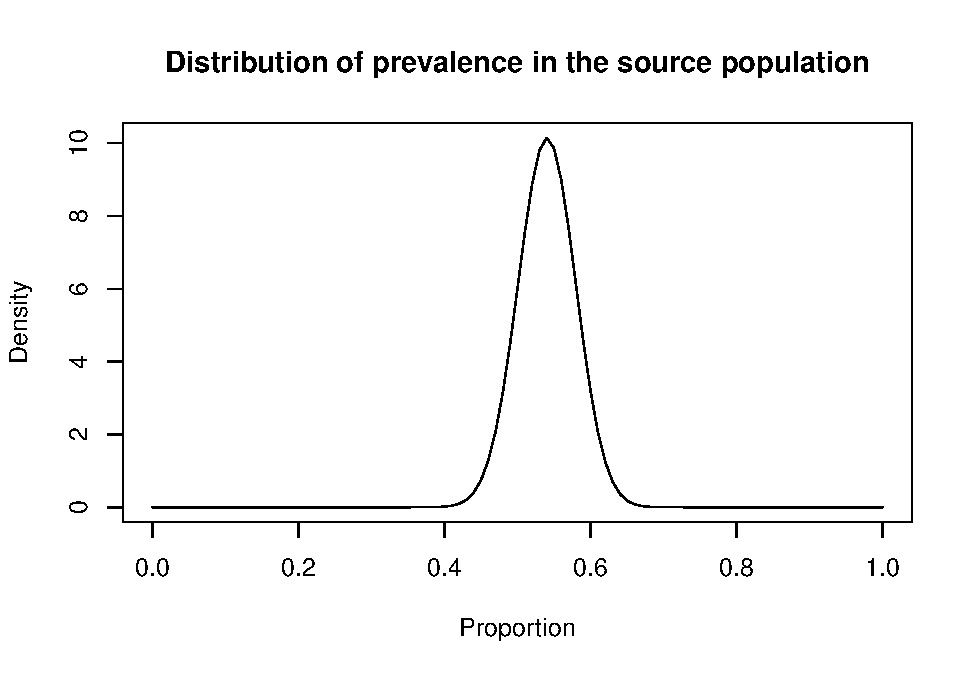
\includegraphics[keepaspectratio]{_main_files/_main_files/figure-latex/unnamed-chunk-66-1.pdf}}

\subsection{Generating informative hyperpriors for mu and psi}\label{generating-informative-hyperpriors-for-mu-and-psi}

\href{https://link.springer.com/article/10.1198/1085711031526}{Hanson et al.~(2003)} proposed to use a \textbf{beta distribution as a hyperprior for \emph{mu} and a gamma distribution for \emph{psi}}. They also provided a method to elicit values for these hyperpriors. This method is, however, slightly more technical than what we have done so far.

\subsubsection{mu}\label{mu}

For \emph{mu}, (the mean within-herd prevalence) we could use a method similar to the one we used before. For instance, we could have some literature, external data, or experts opinion, indicating a most likely (mode) mean within-herd prevalence in the source population, and we could provide the 97.5th (or another) percentile for this mean within-herd prevalence. As an example, in the PAG \emph{vs.} ultrasound study, \href{https://www.sciencedirect.com/science/article/pii/S016758771630527X?via\%3Dihub}{Dufour et al.~(2017)} used reproductive data from 30 other herds from the same region as the 18 recruited herds. They computed the within-herd pregnancy prevalence at testing for these 30 herds and found a 50th and 95th percentiles of 42\% and 74\%, respectively. Using the \texttt{epiR} \texttt{epi.betabuster} function we could find the corresponding beta distribution as follow:

\begin{Shaded}
\begin{Highlighting}[]
\FunctionTok{library}\NormalTok{(epiR) }
\CommentTok{\# Prevalence as Mode=0.42, and we are 95\% sure \textless{}0.74 }
\NormalTok{rval }\OtherTok{\textless{}{-}} \FunctionTok{epi.betabuster}\NormalTok{(}\AttributeTok{mode=}\FloatTok{0.42}\NormalTok{, }
                       \AttributeTok{conf=}\FloatTok{0.95}\NormalTok{, }
                       \AttributeTok{imsure=}\StringTok{"less than"}\NormalTok{, }
                       \AttributeTok{x=}\FloatTok{0.74}\NormalTok{)  }

\NormalTok{rval}\SpecialCharTok{$}\NormalTok{shape1                }\CommentTok{\#View the a shape parameter in rval}
\end{Highlighting}
\end{Shaded}

\begin{verbatim}
## [1] 3.132
\end{verbatim}

\begin{Shaded}
\begin{Highlighting}[]
\NormalTok{rval}\SpecialCharTok{$}\NormalTok{shape2                }\CommentTok{\#View the b shape parameter in rval}
\end{Highlighting}
\end{Shaded}

\begin{verbatim}
## [1] 3.94419
\end{verbatim}

\begin{Shaded}
\begin{Highlighting}[]
\CommentTok{\#Assign the generated values for later usage. }
\NormalTok{mu.shapea }\OtherTok{\textless{}{-}}\NormalTok{ rval}\SpecialCharTok{$}\NormalTok{shape1}
\NormalTok{mu.shapeb }\OtherTok{\textless{}{-}}\NormalTok{ rval}\SpecialCharTok{$}\NormalTok{shape2  }

\CommentTok{\#plot the prior distribution}
\FunctionTok{curve}\NormalTok{(}\FunctionTok{dbeta}\NormalTok{(x, }
            \AttributeTok{shape1=}\NormalTok{mu.shapea, }
            \AttributeTok{shape2=}\NormalTok{mu.shapeb), }
      \AttributeTok{from=}\DecValTok{0}\NormalTok{, }\AttributeTok{to=}\DecValTok{1}\NormalTok{, }
      \AttributeTok{main=}\StringTok{"Hyperprior for mu (the mean within{-}herd prevalence)"}\NormalTok{, }
      \AttributeTok{xlab =} \StringTok{"Proportion"}\NormalTok{, }
      \AttributeTok{ylab =} \StringTok{"Density"}\NormalTok{)}
\end{Highlighting}
\end{Shaded}

\pandocbounded{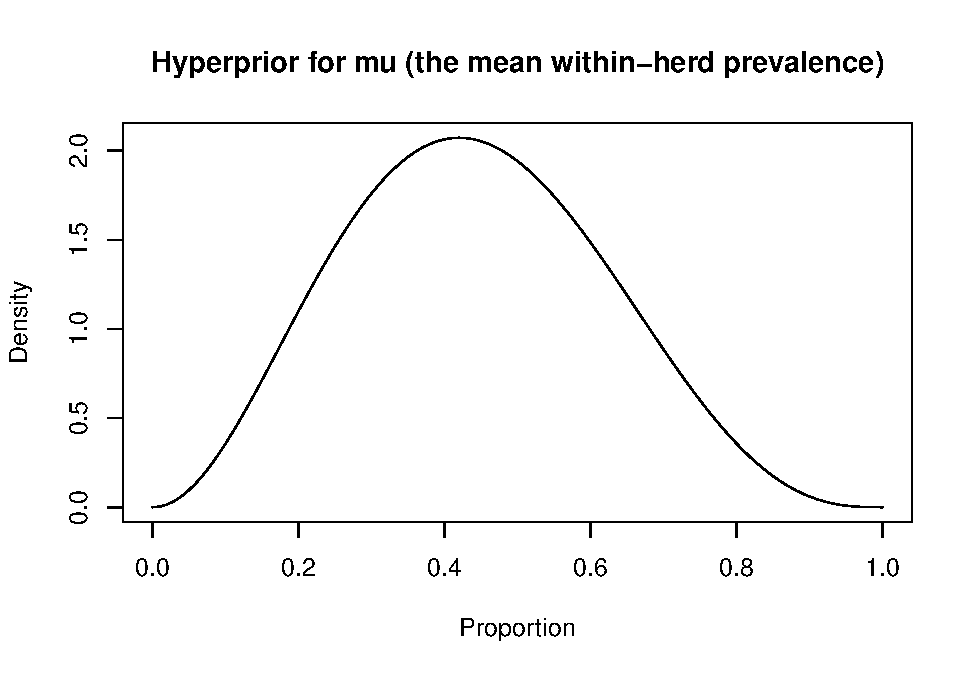
\includegraphics[keepaspectratio]{_main_files/_main_files/figure-latex/unnamed-chunk-67-1.pdf}}

\subsubsection{psi}\label{psi}

For \emph{psi}, which describe the spread of the distribution around the mean within-herd prevalence, \href{https://link.springer.com/article/10.1198/1085711031526}{Hanson et al.~(2003)} proposed to describe the uncertainty around the 90th percentile of the distribution of the mean within-herd prevalence. More specifically, they proposed to use the most likely value (mode) for that 90th percentile and a less likely and large value (for instance the 90th percentile) of this 90th percentile.

For instance, in \href{https://www.sciencedirect.com/science/article/pii/S016758771630527X?via\%3Dihub}{Dufour et al.~(2017)}, using the 30 herds from the same region, they found a 90th percentile of 65\% of pregnancy (i.e., the top 10\% of herds would achieve 65\% pregnancy rate at pregnancy testing). Through experts opinion, they identified that this 90th percentile could hardly be higher than 75\%, thus a 90th percentile of the 90th percentile of 75\%. In other words, they proposed that the top 10\% of herds would most probably have a pregnancy rate at testing of 65\%, but this could possibly (90\% sure) be up to 75\%.

Then, as described by \href{https://link.springer.com/article/10.1198/1085711031526}{Hanson et al.~(2003)}, the 50th percentile of the gamma distribution for \emph{psi} can be computed by adding the \emph{a} and \emph{b} terms of the \emph{beta(a, b)} distribution with mean of 42\% (based on \emph{mu}'s mode) and 90th percentile of 65\% (based on the above assumption on the median value for the 90th percentile).

\begin{Shaded}
\begin{Highlighting}[]
\NormalTok{fifty.psi }\OtherTok{\textless{}{-}} \FunctionTok{epi.betabuster}\NormalTok{(}\AttributeTok{mode=}\FloatTok{0.42}\NormalTok{, }
                            \AttributeTok{conf =} \FloatTok{0.90}\NormalTok{, }
                            \AttributeTok{imsure=}\StringTok{"less than"}\NormalTok{, }
                            \AttributeTok{x=}\FloatTok{0.65}\NormalTok{)  }

\CommentTok{\# Computing the value for the 50th percentile for the gamma distribution for psi }
\NormalTok{fifty }\OtherTok{\textless{}{-}}\NormalTok{ fifty.psi}\SpecialCharTok{$}\NormalTok{shape1 }\SpecialCharTok{+}\NormalTok{ fifty.psi}\SpecialCharTok{$}\NormalTok{shape2 }
\NormalTok{fifty}
\end{Highlighting}
\end{Shaded}

\begin{verbatim}
## [1] 8.904762
\end{verbatim}

The 90th percentile of the gamma distribution is computed in the same manner, but using the \emph{a} and \emph{b} terms of the \emph{beta(a, b)} distribution with mean of, again, 42\%, but 90th percentile of 75\%.

\begin{Shaded}
\begin{Highlighting}[]
\NormalTok{ninety.psi }\OtherTok{\textless{}{-}} \FunctionTok{epi.betabuster}\NormalTok{(}\AttributeTok{mode=}\FloatTok{0.42}\NormalTok{, }
                            \AttributeTok{conf =} \FloatTok{0.90}\NormalTok{, }
                            \AttributeTok{imsure=}\StringTok{"less than"}\NormalTok{, }
                            \AttributeTok{x=}\FloatTok{0.75}\NormalTok{)  }

\CommentTok{\# Computing the value for the 50th percentile for the gamma distribution for psi }
\NormalTok{ninety }\OtherTok{\textless{}{-}}\NormalTok{ ninety.psi}\SpecialCharTok{$}\NormalTok{shape1 }\SpecialCharTok{+}\NormalTok{ fifty.psi}\SpecialCharTok{$}\NormalTok{shape2 }
\NormalTok{ninety}
\end{Highlighting}
\end{Shaded}

\begin{verbatim}
## [1] 7.037762
\end{verbatim}

Using this methodology, we obtained the 50th and 90th percentiles for the gamma distribution for \emph{psi} of 8.9047619 and 7.0377619, respectively. Finally, these percentiles can be translated to obtain the shape and rate parameters of the corresponding gamma distribution.

To achieve this in R, we can use the \texttt{GammaParmsFromQuantile.R} function that was developed by \href{https://www.medicine.mcgill.ca/epidemiology/Joseph/PBelisle/GammaParmsFromQuantiles.html\#download}{Patrick Brisle from McGill U}. This function is not currently part of \texttt{R} package. It has to be downloaded from \href{https://www.medicine.mcgill.ca/epidemiology/Joseph/PBelisle/GammaParmsFromQuantiles.html\#download}{Patrick Brisle website}. You can save the function on your computer, we did save it in a folder named ``Functions''. In the chunk below, the function is called and then used to identify the two parameters (shape and rate) for \emph{psi}'s gamma distribution.

\begin{Shaded}
\begin{Highlighting}[]
\FunctionTok{source}\NormalTok{(}\StringTok{\textquotesingle{}Functions/GammaParmsFromQuantiles.R\textquotesingle{}}\NormalTok{)}
\NormalTok{psi.gamma }\OtherTok{\textless{}{-}} \FunctionTok{gamma.parms.from.quantiles}\NormalTok{(}\AttributeTok{q=}\FunctionTok{c}\NormalTok{(fifty, ninety), }\AttributeTok{p=}\FunctionTok{c}\NormalTok{(}\FloatTok{0.50}\NormalTok{, }\FloatTok{0.90}\NormalTok{), }\AttributeTok{plot=}\NormalTok{T)}
\end{Highlighting}
\end{Shaded}

\pandocbounded{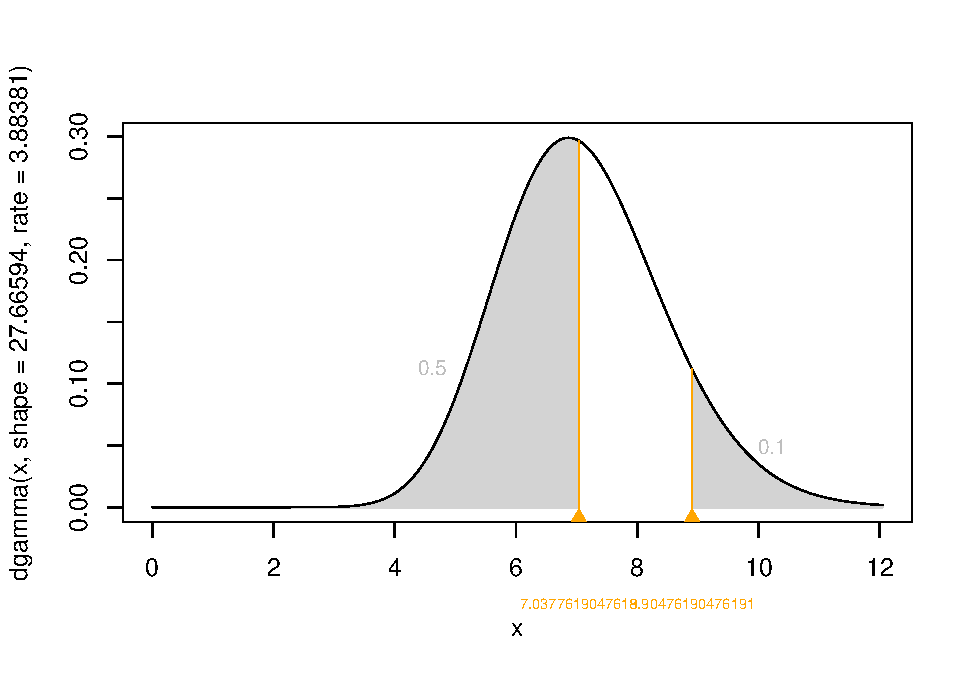
\includegraphics[keepaspectratio]{_main_files/_main_files/figure-latex/unnamed-chunk-70-1.pdf}}

\begin{Shaded}
\begin{Highlighting}[]
\NormalTok{psi.shapea }\OtherTok{\textless{}{-}}\NormalTok{ psi.gamma}\SpecialCharTok{$}\NormalTok{shape   }\CommentTok{\# a shape parameter for gamma}
\NormalTok{psi.shapea}
\end{Highlighting}
\end{Shaded}

\begin{verbatim}
## [1] 27.66594
\end{verbatim}

\begin{Shaded}
\begin{Highlighting}[]
\NormalTok{psi.shapeb }\OtherTok{\textless{}{-}}\NormalTok{ psi.gamma}\SpecialCharTok{$}\NormalTok{rate    }\CommentTok{\# b shape parameter for gamma}
\NormalTok{psi.shapeb}
\end{Highlighting}
\end{Shaded}

\begin{verbatim}
## [1] 3.88381
\end{verbatim}

A gamma (27.7, 3.9) distribution can, therefore, be used to represent hyperprior information on \emph{psi}.

\subsection{Extensions}\label{extensions}

Of course, the hierarchical model presented could be extended as we have seen before to add, for instance, covariance terms between tests (thus, allowing for conditional dependence between tests). We could also extend the likelihood function to compare 3 (or 4, or 5, etc) tests as we will see in Chapter 9.

\chapter{Exercise 3 - Multiple populations}\label{exercise-3---multiple-populations}

\section{Questions}\label{questions-2}

Open up the \texttt{R} project for Exercise 3 (i.e., the R project file named \emph{Exercise 3.Rproj}).

In the Exercise 3 folder, you will find partially completed \texttt{R} scripts. To answer the questions, try to complete the missing parts (they are highlighted by a \textbf{\#TO COMPLETE\#} comment). We also provided complete \texttt{R} scripts, but try to work it out on your own first!

We know that US is not a gold-standard test for diagnosing pregnancy in dairy cows between 28-45 days post-AI. \href{https://www.sciencedirect.com/science/article/pii/S0093691X06001543?via\%3Dihub}{Romano et al.~(2006)} have reported estimates of Se and Sp for US that we have used in the preceding exercises. However, these US accuracy
estimates were themselves computed without comparing to a gold-standard, and the authors did not used a LCM methodology. The reported US accuracy estimates are, thus, possibly biased to some extent.

It would be great if we could compute Se and Sp estimates for the PAG test, but without using these potentially biased US accuracy estimates. In the complete study, we have results for cows from three herds. Assuming that pregnancy prevalence is sufficiently different between herds, we could possibly use the \href{https://www.jstor.org/stable/2530508?seq=1}{Hui and Walter} model with 3 populations. Cross-tabulated PAG and US data from the 3 herds are presented below.

\textbf{Table.} Cross-classified results from the PAG and US diagnostic tests in the three herds studied.

\begin{longtable}[]{@{}
  >{\centering\arraybackslash}p{(\linewidth - 26\tabcolsep) * \real{0.0930}}
  >{\centering\arraybackslash}p{(\linewidth - 26\tabcolsep) * \real{0.0698}}
  >{\centering\arraybackslash}p{(\linewidth - 26\tabcolsep) * \real{0.0698}}
  >{\centering\arraybackslash}p{(\linewidth - 26\tabcolsep) * \real{0.0853}}
  >{\centering\arraybackslash}p{(\linewidth - 26\tabcolsep) * \real{0.0233}}
  >{\centering\arraybackslash}p{(\linewidth - 26\tabcolsep) * \real{0.0930}}
  >{\centering\arraybackslash}p{(\linewidth - 26\tabcolsep) * \real{0.0698}}
  >{\centering\arraybackslash}p{(\linewidth - 26\tabcolsep) * \real{0.0698}}
  >{\centering\arraybackslash}p{(\linewidth - 26\tabcolsep) * \real{0.0853}}
  >{\centering\arraybackslash}p{(\linewidth - 26\tabcolsep) * \real{0.0233}}
  >{\centering\arraybackslash}p{(\linewidth - 26\tabcolsep) * \real{0.0930}}
  >{\centering\arraybackslash}p{(\linewidth - 26\tabcolsep) * \real{0.0698}}
  >{\centering\arraybackslash}p{(\linewidth - 26\tabcolsep) * \real{0.0698}}
  >{\centering\arraybackslash}p{(\linewidth - 26\tabcolsep) * \real{0.0853}}@{}}
\toprule\noalign{}
\begin{minipage}[b]{\linewidth}\centering
\textbf{Herd 1}
\end{minipage} & \begin{minipage}[b]{\linewidth}\centering
\end{minipage} & \begin{minipage}[b]{\linewidth}\centering
\end{minipage} & \begin{minipage}[b]{\linewidth}\centering
\textbf{Total}
\end{minipage} & \begin{minipage}[b]{\linewidth}\centering
\end{minipage} & \begin{minipage}[b]{\linewidth}\centering
\textbf{Herd 2}
\end{minipage} & \begin{minipage}[b]{\linewidth}\centering
\end{minipage} & \begin{minipage}[b]{\linewidth}\centering
\end{minipage} & \begin{minipage}[b]{\linewidth}\centering
\textbf{Total}
\end{minipage} & \begin{minipage}[b]{\linewidth}\centering
\end{minipage} & \begin{minipage}[b]{\linewidth}\centering
\textbf{Herd 3}
\end{minipage} & \begin{minipage}[b]{\linewidth}\centering
\end{minipage} & \begin{minipage}[b]{\linewidth}\centering
\end{minipage} & \begin{minipage}[b]{\linewidth}\centering
\textbf{Total}
\end{minipage} \\
\midrule\noalign{}
\endhead
\bottomrule\noalign{}
\endlastfoot
& \textbf{US+} & \textbf{US-} & & & & \textbf{US+} & \textbf{US-} & & & & \textbf{US+} & \textbf{US-} & \\
\textbf{PAG+} & 138 & 10 & & & \textbf{PAG+} & 71 & 8 & & & \textbf{PAG+} & 46 & 3 & \\
\textbf{PAG-} & 1 & 113 & & & \textbf{PAG-} & 0 & 69 & & & \textbf{PAG-} & 1 & 37 & \\
\textbf{Total} & & & 262 & & \textbf{Total} & & & 148 & & \textbf{Total} & & & 87 \\
\end{longtable}

\textbf{1.} Using a \href{https://www.jstor.org/stable/2530508?seq=1}{Hui and Walter} model with these three populations, how many unknown parameters and degrees of freedom would you have, and how many informative priors will you need?

\textbf{2.} Based on the observed results (do not compute a model yet, just ballpark estimates), do you think pregnancy prevalence differ between the 3 herds? Do you have any biological reason to believe that PAG or US Se and/or Sp should not be the same in herd \#1 \emph{vs.} herd \#2 \emph{vs.} herd \#3?

\textbf{3. Start from the partially completed \emph{Question 3.R} script located in Exercise 3 folder.} Try to apply a \href{https://www.jstor.org/stable/2530508?seq=1}{Hui and Walter} model for three populations to these data using informative pregnancy prevalence (mode=0.42, 97.5th percentile=0.74) and informative US accuracy priors (Se: mode=0.90, 2.5th percentile=0.85; Sp: mode=0.95, 2.5th percentile=0.90). For this analysis, consider that the two tests are conditionally independent. Then use the same LCM, but with vague priors for all parameters and compare your results.

\section{Answers}\label{answers-2}

\textbf{1.} Using a \href{https://www.jstor.org/stable/2530508?seq=1}{Hui and Walter} model with these three populations, how many unknown parameters and degrees of freedom would you have, and how many informative priors will you need?

\textbf{Answer:} We would still have 2 Se and 2 Sp and now 3 prevalence (one for each herd) to estimate, thus 7 unknown parameters. For each herd we have 3 degrees of freedom; in total 9 degrees of freedom. We have 7 unknown parameters and 9 degrees of freedom, so we do not need any informative prior to estimate these parameters.

\textbf{2.} Based on the observed results (do not compute a model yet, just ballpark estimates), do you think pregnancy prevalence differ between the 3 herds? Do you have any biological reason to believe that PAG or US Se and/or Sp should not be the same in herd \#1 \emph{vs.} herd \#2 \emph{vs.} herd \#3?

\textbf{Answer:} We do not know the true pregnancy prevalence in these herds, but we could explore the apparent prevalence observed using our tests under investigation. Here are the apparent prevalence estimates computed using either PAG or US results by herd.

\textbf{Table.} Apparent prevalence of pregnancy in 3 herds using either a PAG or US test.

\begin{longtable}[]{@{}ccc@{}}
\toprule\noalign{}
\textbf{Herd} & \textbf{PAG-based prevalence} & \textbf{US-based prevalence} \\
\midrule\noalign{}
\endhead
\bottomrule\noalign{}
\endlastfoot
\textbf{1} & 0.56 & 0.53 \\
\textbf{2} & 0.53 & 0.48 \\
\textbf{3} & 0.56 & 0.54 \\
\end{longtable}

These prevalences are fairly similar\ldots{} In a real-life situation, I would probably try to find another way to split the dataset in different populations so we have more striking outcome prevalence differences between populations (e.g., cows with \textless{} 3 AI \emph{vs.} cows with ≥ 3 AI; 1st lactation cows \emph{vs.} older cows). But, for the sake of the exercise, we could still try to apply the \href{https://www.jstor.org/stable/2530508?seq=1}{Hui and Walter} model to these data.

Regarding PAG or US changing Se and/or Sp between the three herds, it is difficult to imagine any reason that would affect PAG or US accuracy from one herd to another. We would probably be OK considering that, no matter the herd, tests Se and Sp are the same.

\textbf{3.} Try to apply a \href{https://www.jstor.org/stable/2530508?seq=1}{Hui and Walter} model for three populations to these data using informative pregnancy prevalence (mode=0.42, 97.5th percentile=0.74) and informative US accuracy priors (Se: mode=0.90, 2.5th percentile=0.85; Sp: mode=0.95, 2.5th percentile=0.90). For this analysis, consider that the two tests are conditionally independent. Then use the same LCM, but with vague priors for all parameters and compare your results.

\textbf{Answer:} The model with informative priors run very smoothly, as expected.

The model using vague priors for all parameters also converged very easily, autocorrelation is not a problem, etc. Isn't it a bit surprising? We would have expected that, with prevalence that are not overly different between the three herds, using the \href{https://www.jstor.org/stable/2530508?seq=1}{Hui and Walter} model would not necessarily make the model identifiable. In this specific example, however, we have two very precise tests and, therefore, limited disagreement between tests (check the three 2x2 tables). Therefore, the number of potential solutions is very limited and the model is still identifiable even though we do not have striking prevalence differences between herds. It may not work as well in a different dataset. Below, I have summarize the results of the LCM with informative \emph{vs.} vague priors.

\textbf{Table.} Results from a 2 tests, 3 populations LCM using different priors (informative on pregnancy prevalence and on US Se and Sp \emph{vs.} vague priors on all parameters).

\begin{longtable}[]{@{}
  >{\centering\arraybackslash}p{(\linewidth - 10\tabcolsep) * \real{0.1500}}
  >{\centering\arraybackslash}p{(\linewidth - 10\tabcolsep) * \real{0.1700}}
  >{\centering\arraybackslash}p{(\linewidth - 10\tabcolsep) * \real{0.2200}}
  >{\centering\arraybackslash}p{(\linewidth - 10\tabcolsep) * \real{0.0700}}
  >{\centering\arraybackslash}p{(\linewidth - 10\tabcolsep) * \real{0.1700}}
  >{\centering\arraybackslash}p{(\linewidth - 10\tabcolsep) * \real{0.2200}}@{}}
\toprule\noalign{}
\begin{minipage}[b]{\linewidth}\centering
\textbf{Parameter}
\end{minipage} & \begin{minipage}[b]{\linewidth}\centering
\textbf{Informative}
\end{minipage} & \begin{minipage}[b]{\linewidth}\centering
\end{minipage} & \begin{minipage}[b]{\linewidth}\centering
\end{minipage} & \begin{minipage}[b]{\linewidth}\centering
\textbf{Vague}
\end{minipage} & \begin{minipage}[b]{\linewidth}\centering
\end{minipage} \\
\midrule\noalign{}
\endhead
\bottomrule\noalign{}
\endlastfoot
& \textbf{Prior} & \textbf{Posterior} & & \textbf{Prior} & \textbf{Posterior} \\
\textbf{Prev1} & Beta(4.2, 5.4) & 0.554 (0.493, 0.614) & & Beta (1.0, 1.0) & 0.547 (0.482, 0.612) \\
\textbf{Prev2} & Beta(4.2, 5.4) & 0.517 (0.436, 0.595) & & Beta (1.0, 1.0) & 0.505 (0.418, 0.590) \\
\textbf{Prev3} & Beta(4.2, 5.4) & 0.547 (0.444, 0.646) & & Beta (1.0, 1.0) & 0.551 (0.445, 0.654) \\
\textbf{Se US} & Beta (100, 12) & 0.926 (0.893, 0.955) & & Beta (1.0, 1.0) & 0.961 (0.908, 0.998) \\
\textbf{Sp US} & Beta (100, 6.2) & 0.977 (0.956, 0.990) & & Beta (1.0, 1.0) & 0.993 (0.972, 1.000) \\
\textbf{Se PAG} & Beta (1.0, 1.0) & 0.996 (0.980, 1.000) & & Beta (1.0, 1.0) & 0.994 (0.976, 1.000) \\
\textbf{Sp PAG} & Beta (1.0, 1.0) & 0.980 (0.956, 0.990) & & Beta (1.0, 1.0) & 0.949 (0.891, 0.997) \\
\end{longtable}

We have small difference between approaches. In the LCM with informative priors, we indicated, as prior knowledge, that US Se and Sp were around 0.90 and 0.95, respectively. Our posterior estimates for these parameters were 0.93 and 0.98. So, our data indicates that US Se and Sp is possibly better than what was reported by \href{https://www.sciencedirect.com/science/article/pii/S0093691X06001543?via\%3Dihub}{Romano et al.}. This is confirmed in the model where we used vague priors. In that latter LCM, US Se and Sp were estimated at 0.96 and 0.99, respectively.

In the LCM with vague priors, Se of US was estimated to 0.96 (\emph{vs.} 0.93), as a result, the PAG Sp was slightly reduced (0.95 \emph{vs.} 0.98). In other words, in the LCM with informative priors, most of the US-/PAG+ results were attributed to errors of the US exam (because of the prior US Se with mode of 0.90). In the LCM with vague priors, the US-/PAG+ disagreements were distributed more equally between an error of the PAG \emph{vs.} an error of the US test.

\chapter{Multiple diagnostic tests}\label{multiple-diagnostic-tests}

In some situations, individuals will be tested using more than two diagnostic tests. For instance, if all individuals were tested using three different diagnostic tests (Test A, Test B, and Test C) we could present the cross-classified results of the three tests as follows:

\textbf{Table.} Cross-classified results from three diagnostic tests in one population.

\begin{longtable}[]{@{}
  >{\centering\arraybackslash}p{(\linewidth - 12\tabcolsep) * \real{0.1605}}
  >{\centering\arraybackslash}p{(\linewidth - 12\tabcolsep) * \real{0.1605}}
  >{\centering\arraybackslash}p{(\linewidth - 12\tabcolsep) * \real{0.1605}}
  >{\centering\arraybackslash}p{(\linewidth - 12\tabcolsep) * \real{0.0370}}
  >{\centering\arraybackslash}p{(\linewidth - 12\tabcolsep) * \real{0.1605}}
  >{\centering\arraybackslash}p{(\linewidth - 12\tabcolsep) * \real{0.1605}}
  >{\centering\arraybackslash}p{(\linewidth - 12\tabcolsep) * \real{0.1605}}@{}}
\toprule\noalign{}
\begin{minipage}[b]{\linewidth}\centering
\textbf{Test C+}
\end{minipage} & \begin{minipage}[b]{\linewidth}\centering
\end{minipage} & \begin{minipage}[b]{\linewidth}\centering
\end{minipage} & \begin{minipage}[b]{\linewidth}\centering
\end{minipage} & \begin{minipage}[b]{\linewidth}\centering
\textbf{Test C-}
\end{minipage} & \begin{minipage}[b]{\linewidth}\centering
\end{minipage} & \begin{minipage}[b]{\linewidth}\centering
\end{minipage} \\
\midrule\noalign{}
\endhead
\bottomrule\noalign{}
\endlastfoot
& \textbf{Test A+} & \textbf{Test A-} & & & \textbf{Test A+} & \textbf{Test A-} \\
\textbf{Test B+} & n1 & n3 & & \textbf{Test B+} & n5 & n7 \\
\textbf{Test B-} & n2 & n4 & & \textbf{Test B-} & n6 & n8 \\
\end{longtable}

Contrarily to the case where we had two tests in 2 populations, we can see from the preceding table that we have 7 degrees of freedom available. Indeed, we need to know the total number of individuals (\emph{n}) and the content of seven of the eight cells to ``guess'' the value in the last cell. Moreover, with three diagnostic tests, we would have seven unknown parameters (\emph{SeA} and \emph{SpA}, \emph{SeB} and \emph{SpB}, \emph{SeC} and \emph{SpC},and the population's prevalence, \emph{P}) to estimate. The model is, therefore, identifiable. Again, we can refer to \href{https://doi.org/10.20506/rst.40.1.3224}{Cheung et al.~(2021)} to describe how the number of unknown parameters and degrees of freedom vary as function of the number of diagnostic tests used (see below).

\textbf{Table.} Number of degrees of freedom and of unknown parameters when comparing an increasing number of conditionally independent diagnostic tests in one single population (adapted from \href{https://doi.org/10.20506/rst.40.1.3224}{Cheung et al.~(2021)}).

\begin{longtable}[]{@{}
  >{\centering\arraybackslash}p{(\linewidth - 6\tabcolsep) * \real{0.1419}}
  >{\centering\arraybackslash}p{(\linewidth - 6\tabcolsep) * \real{0.2635}}
  >{\centering\arraybackslash}p{(\linewidth - 6\tabcolsep) * \real{0.2635}}
  >{\centering\arraybackslash}p{(\linewidth - 6\tabcolsep) * \real{0.3311}}@{}}
\toprule\noalign{}
\begin{minipage}[b]{\linewidth}\centering
\textbf{Number of Tests}
\end{minipage} & \begin{minipage}[b]{\linewidth}\centering
\textbf{Number of unknown parameters (np)}
\end{minipage} & \begin{minipage}[b]{\linewidth}\centering
\textbf{Number of degrees of freedom (df)}
\end{minipage} & \begin{minipage}[b]{\linewidth}\centering
\textbf{Minimum number of informative priors needed}
\end{minipage} \\
\midrule\noalign{}
\endhead
\bottomrule\noalign{}
\endlastfoot
2 & 5 & 3 & 2 \\
3 & 7 & 7 & 0 \\
4 & 9 & 15 & 0 \\
k & 2*k+1 & 2\^{}k -1 & if df \textless{} np, then np-df \\
\end{longtable}

As you can see, adding diagnostic tests could be an extremely valuable option to make a LCM identifiable. The gain in statistical power, however, will be maximized if:

-We used many \textbf{conditionally independent} diagnostic tests\\
-The sample size is sufficient so \textbf{all tests combinations are represented} (i.e., no empty cells in the table presenting the cross-classified results)

\section{Likelihood function with 3 tests}\label{likelihood-function-with-3-tests}

With three diagnostic tests applied to a single population, the likelihood function that could be used to link the observed data (\emph{n1}, \ldots, \emph{n8}) to the unknown parameters (\emph{SeA} and \emph{SpA}, \emph{SeB} and \emph{SpB}, \emph{SeC} and \emph{SpC},and \emph{P}) can be described as follows:

\(n[1:8] \sim dmulti(P[1:8], n)\)

\(P1 = P*SeA*SeB*SeC + (1-P)*(1-SpA)*(1-SpB)*(1-SpC)\)\\
\(P2 = P*SeA*(1-SeB)*SeC + (1-P)*(1-SpA)*SpB*(1-SpC)\)\\
\(P3 = P*(1-SeA)*SeB*SeC + (1-P)*SpA*(1-SpB)*(1-SpC)\)\\
\(P4 = P*(1-SeA)*(1-SeB)*SeC + (1-P)*SpA*SpB*(1-SpC)\)\\
\(P5 = P*SeA*SeB*(1-SeC) + (1-P)*(1-SpA)*(1-SpB)*SpC\)\\
\(P6 = P*SeA*(1-SeB)*(1-SeC) + (1-P)*(1-SpA)*SpB*SpC\)\\
\(P7 = P*(1-SeA)*SeB*(1-Sec) + (1-P)*SpA*(1-SpB)*SpC\)\\
\(P8 = P*(1-SeA)*(1-SeB)*(1-SeC) + (1-P)*SpA*SpB*SpC\)

Again, if we put that in words, the number of individuals in cell \emph{n1} (i.e., TestA+ and TestB+ and TestC+) is determined by the number of individuals tested (\emph{n}) and the probability (\emph{P1}) of falling in that cell. The latter itself depends on the true prevalence of disease in the population (\emph{P}), and on each of the tests sensitivity (\emph{SeA}, \emph{SeB}, and \emph{SeC}) and specificity (\emph{SpA}, \emph{SpB}, and \emph{SpC}). We can use similar reasoning for \emph{n2} to \emph{n8}. Finally, the multinomial distribution would further impose that the eight probabilities (\emph{P1} to \emph{P8}) have to sum up to 1.0 (i.e., 100\%).

\section{Organizing the data with 3 tests}\label{organizing-the-data-with-3-tests}

To run such a model, we simply need to provide a dataset where \emph{n1}, \emph{n2}, \emph{n3}, \emph{n4}, \emph{n5}, \emph{n6}, \emph{n7}, and \emph{n8} are listed (in that order). For instance, in the PAG \emph{vs.} US study, we have a number of cows that also had a conventional transrectal exam (\textbf{TRE}). The results of the three tests can be presented as follows:

\textbf{Table.} Cross-classified results from a PAG, US, and TRE diagnostic tests in one population.

\begin{longtable}[]{@{}ccccccc@{}}
\toprule\noalign{}
\textbf{TRE+} & & & & \textbf{TRE-} & & \\
\midrule\noalign{}
\endhead
\bottomrule\noalign{}
\endlastfoot
& \textbf{US+} & \textbf{US-} & & & \textbf{US+} & \textbf{US-} \\
\textbf{PAG+} & 240 & 12 & & \textbf{PAG+} & 15 & 9 \\
\textbf{PAG-} & 1 & 2 & & \textbf{PAG-} & 1 & 216 \\
\end{longtable}

The dataset could, thus be created as follows:

\begin{Shaded}
\begin{Highlighting}[]
\CommentTok{\#n is of the form : (TestA+ TestB+ Test C+), (TestA+ TestB{-} TestC+), (TestA{-} TestB+ TestC+), (TestA{-} TestB{-} TestC+), (TestA+ TestB+ TestC{-}), (TestA+ TestB{-} TestC{-}), (TestA{-} TestB+ TestC{-}), (TestA{-} Test{-} TestC{-})}
\NormalTok{datalist }\OtherTok{\textless{}{-}} \FunctionTok{list}\NormalTok{(}\AttributeTok{n=}\FunctionTok{c}\NormalTok{(}\DecValTok{240}\NormalTok{, }\DecValTok{1}\NormalTok{, }\DecValTok{12}\NormalTok{, }\DecValTok{2}\NormalTok{, }\DecValTok{15}\NormalTok{, }\DecValTok{1}\NormalTok{, }\DecValTok{9}\NormalTok{, }\DecValTok{216}\NormalTok{))}
\end{Highlighting}
\end{Shaded}

\section{The JAGS model with 3 tests}\label{the-jags-model-with-3-tests}

Again, we could provide the values that will be used to describe the prior distributions as we did before (they will then become included in the LCM text file). The only difference is that we now have three Se and Sp to describe. In the example below, I will use vague priors for all parameters.

\begin{Shaded}
\begin{Highlighting}[]
\CommentTok{\#We could first create labels for TestA, TestB, and TestC}
\NormalTok{TestA }\OtherTok{\textless{}{-}} \StringTok{"US"}
\NormalTok{TestB }\OtherTok{\textless{}{-}} \StringTok{"PAG"}
\NormalTok{TestC }\OtherTok{\textless{}{-}} \StringTok{"TRE"}

\CommentTok{\#Provide information for the prior distributions (all beta distributions) for the 7 unknown parameters }
\NormalTok{Prev.shapea }\OtherTok{\textless{}{-}} \DecValTok{1}         \CommentTok{\#a shape parameter for Prev     }
\NormalTok{Prev.shapeb }\OtherTok{\textless{}{-}} \DecValTok{1}         \CommentTok{\#b shape parameter for Prev }

\NormalTok{Se.TestA.shapea }\OtherTok{\textless{}{-}} \DecValTok{1}     \CommentTok{\#a shape parameter for Se of TestA}
\NormalTok{Se.TestA.shapeb }\OtherTok{\textless{}{-}} \DecValTok{1}     \CommentTok{\#b shape parameter for Se of TestA}
\NormalTok{Sp.TestA.shapea }\OtherTok{\textless{}{-}} \DecValTok{1}     \CommentTok{\#a shape parameter for Sp of TestA}
\NormalTok{Sp.TestA.shapeb }\OtherTok{\textless{}{-}} \DecValTok{1}     \CommentTok{\#b shape parameter for Sp of TestA}

\NormalTok{Se.TestB.shapea }\OtherTok{\textless{}{-}} \DecValTok{1}     \CommentTok{\#a shape parameter for Se of TestB}
\NormalTok{Se.TestB.shapeb }\OtherTok{\textless{}{-}} \DecValTok{1}     \CommentTok{\#b shape parameter for Se of TestB}
\NormalTok{Sp.TestB.shapea }\OtherTok{\textless{}{-}} \DecValTok{1}     \CommentTok{\#a shape parameter for Sp of TestB}
\NormalTok{Sp.TestB.shapeb }\OtherTok{\textless{}{-}} \DecValTok{1}     \CommentTok{\#b shape parameter for Sp of TestB}

\NormalTok{Se.TestC.shapea }\OtherTok{\textless{}{-}} \DecValTok{1}     \CommentTok{\#a shape parameter for Se of TestC}
\NormalTok{Se.TestC.shapeb }\OtherTok{\textless{}{-}} \DecValTok{1}     \CommentTok{\#b shape parameter for Se of TestC}
\NormalTok{Sp.TestC.shapea }\OtherTok{\textless{}{-}} \DecValTok{1}     \CommentTok{\#a shape parameter for Sp of TestC}
\NormalTok{Sp.TestC.shapeb }\OtherTok{\textless{}{-}} \DecValTok{1}     \CommentTok{\#b shape parameter for Sp of TestC}

\CommentTok{\#I will also need the total number of individuals tested }
\NormalTok{n }\OtherTok{\textless{}{-}} \FunctionTok{sapply}\NormalTok{(datalist, sum)}
\end{Highlighting}
\end{Shaded}

We now have everything that is needed to write the JAGS model.

\begin{Shaded}
\begin{Highlighting}[]
\CommentTok{\#Create the JAGS text file}
\NormalTok{model\_3tests\_1pop\_indep }\OtherTok{\textless{}{-}} \FunctionTok{paste0}\NormalTok{(}\StringTok{"model\{}

\StringTok{\#=== LIKELIHOOD ===\#}

\StringTok{  n[1:8] \textasciitilde{} dmulti(p[1:8], "}\NormalTok{,n,}\StringTok{")}
\StringTok{  p[1] \textless{}{-} Prev*Se\_"}\NormalTok{, TestA, }\StringTok{"*Se\_"}\NormalTok{, TestB, }\StringTok{"*Se\_"}\NormalTok{, TestC, }\StringTok{" + (1{-}Prev)*(1{-}Sp\_"}\NormalTok{, TestA, }\StringTok{")*(1{-}Sp\_"}\NormalTok{, TestB, }\StringTok{")*(1{-}Sp\_"}\NormalTok{, TestC,}\StringTok{")}
\StringTok{  p[2] \textless{}{-} Prev*Se\_"}\NormalTok{, TestA, }\StringTok{"*(1{-}Se\_"}\NormalTok{, TestB, }\StringTok{")*Se\_"}\NormalTok{, TestC, }\StringTok{" + (1{-}Prev)*(1{-}Sp\_"}\NormalTok{, TestA, }\StringTok{")*Sp\_"}\NormalTok{, TestB, }\StringTok{"*(1{-}Sp\_"}\NormalTok{, TestC,}\StringTok{")}
\StringTok{  p[3] \textless{}{-} Prev*(1{-}Se\_"}\NormalTok{, TestA, }\StringTok{")*Se\_"}\NormalTok{, TestB, }\StringTok{"*Se\_"}\NormalTok{, TestC, }\StringTok{" + (1{-}Prev)*Sp\_"}\NormalTok{, TestA, }\StringTok{"*(1{-}Sp\_"}\NormalTok{, TestB, }\StringTok{")*(1{-}Sp\_"}\NormalTok{, TestC,}\StringTok{")}
\StringTok{  p[4] \textless{}{-} Prev*(1{-}Se\_"}\NormalTok{, TestA, }\StringTok{")*(1{-}Se\_"}\NormalTok{, TestB, }\StringTok{")*Se\_"}\NormalTok{, TestC, }\StringTok{" + (1{-}Prev)*Sp\_"}\NormalTok{, TestA, }\StringTok{"*Sp\_"}\NormalTok{, TestB, }\StringTok{"*(1{-}Sp\_"}\NormalTok{, TestC,}\StringTok{")}
\StringTok{  }
\StringTok{  p[5] \textless{}{-} Prev*Se\_"}\NormalTok{, TestA, }\StringTok{"*Se\_"}\NormalTok{, TestB, }\StringTok{"*(1{-}Se\_"}\NormalTok{, TestC,}\StringTok{") + (1{-}Prev)*(1{-}Sp\_"}\NormalTok{, TestA, }\StringTok{")*(1{-}Sp\_"}\NormalTok{, TestB, }\StringTok{")*Sp\_"}\NormalTok{, TestC,}\StringTok{"}
\StringTok{  p[6] \textless{}{-} Prev*Se\_"}\NormalTok{, TestA, }\StringTok{"*(1{-}Se\_"}\NormalTok{, TestB, }\StringTok{")*(1{-}Se\_"}\NormalTok{, TestC,}\StringTok{") + (1{-}Prev)*(1{-}Sp\_"}\NormalTok{, TestA, }\StringTok{")*Sp\_"}\NormalTok{, TestB, }\StringTok{"*Sp\_"}\NormalTok{, TestC,}\StringTok{"}
\StringTok{  p[7] \textless{}{-} Prev*(1{-}Se\_"}\NormalTok{, TestA, }\StringTok{")*Se\_"}\NormalTok{, TestB, }\StringTok{"*(1{-}Se\_"}\NormalTok{, TestC,}\StringTok{") + (1{-}Prev)*Sp\_"}\NormalTok{, TestA, }\StringTok{"*(1{-}Sp\_"}\NormalTok{, TestB, }\StringTok{")*Sp\_"}\NormalTok{, TestC,}\StringTok{"}
\StringTok{  p[8] \textless{}{-} Prev*(1{-}Se\_"}\NormalTok{, TestA, }\StringTok{")*(1{-}Se\_"}\NormalTok{, TestB, }\StringTok{")*(1{-}Se\_"}\NormalTok{, TestC,}\StringTok{") + (1{-}Prev)*Sp\_"}\NormalTok{, TestA, }\StringTok{"*Sp\_"}\NormalTok{, TestB, }\StringTok{"*Sp\_"}\NormalTok{, TestC,}\StringTok{"}
\StringTok{  }
\StringTok{  }
\StringTok{\#=== PRIOR  ===\#}

\StringTok{  Prev \textasciitilde{} dbeta("}\NormalTok{,Prev.shapea,}\StringTok{", "}\NormalTok{,Prev.shapeb,}\StringTok{")    \#\# Prior for Prevalence}
\StringTok{  Se\_"}\NormalTok{, TestA, }\StringTok{" \textasciitilde{} dbeta("}\NormalTok{,Se.TestA.shapea,}\StringTok{", "}\NormalTok{,Se.TestA.shapeb,}\StringTok{")  \#\# Prior for Se of Test A}
\StringTok{  Sp\_"}\NormalTok{, TestA, }\StringTok{" \textasciitilde{} dbeta("}\NormalTok{,Sp.TestA.shapea,}\StringTok{", "}\NormalTok{,Sp.TestA.shapeb,}\StringTok{")  \#\# Prior for Sp of Test A}
\StringTok{  Se\_"}\NormalTok{, TestB, }\StringTok{" \textasciitilde{} dbeta("}\NormalTok{,Se.TestB.shapea,}\StringTok{", "}\NormalTok{,Se.TestB.shapeb,}\StringTok{")  \#\# Prior for Se of Test B}
\StringTok{  Sp\_"}\NormalTok{, TestB, }\StringTok{" \textasciitilde{} dbeta("}\NormalTok{,Sp.TestB.shapea,}\StringTok{", "}\NormalTok{,Sp.TestB.shapeb,}\StringTok{")  \#\# Prior for Sp of Test B}
\StringTok{  Se\_"}\NormalTok{, TestC, }\StringTok{" \textasciitilde{} dbeta("}\NormalTok{,Se.TestC.shapea,}\StringTok{", "}\NormalTok{,Se.TestC.shapeb,}\StringTok{")  \#\# Prior for Se of Test C}
\StringTok{  Sp\_"}\NormalTok{, TestC, }\StringTok{" \textasciitilde{} dbeta("}\NormalTok{,Sp.TestC.shapea,}\StringTok{", "}\NormalTok{,Sp.TestC.shapeb,}\StringTok{")  \#\# Prior for Sp of Test C}
\StringTok{  }
\StringTok{\}"}\NormalTok{)}

\CommentTok{\#write as a text (.txt) file}
\FunctionTok{write.table}\NormalTok{(model\_3tests\_1pop\_indep, }
            \AttributeTok{file=}\StringTok{"model\_3tests\_1pop\_indep.txt"}\NormalTok{, }
            \AttributeTok{quote=}\ConstantTok{FALSE}\NormalTok{, }
            \AttributeTok{sep=}\StringTok{""}\NormalTok{, }
            \AttributeTok{row.names=}\ConstantTok{FALSE}\NormalTok{,}
            \AttributeTok{col.names=}\ConstantTok{FALSE}\NormalTok{)}
\end{Highlighting}
\end{Shaded}

With this code, you could, again, simply modify the labels for Test A, Test B, and Test C, and the shape parameters for the prior distributions. The text file with the JAGS model will automatically be updated. Currently, it looks like this:

\begin{figure}
\centering
\pandocbounded{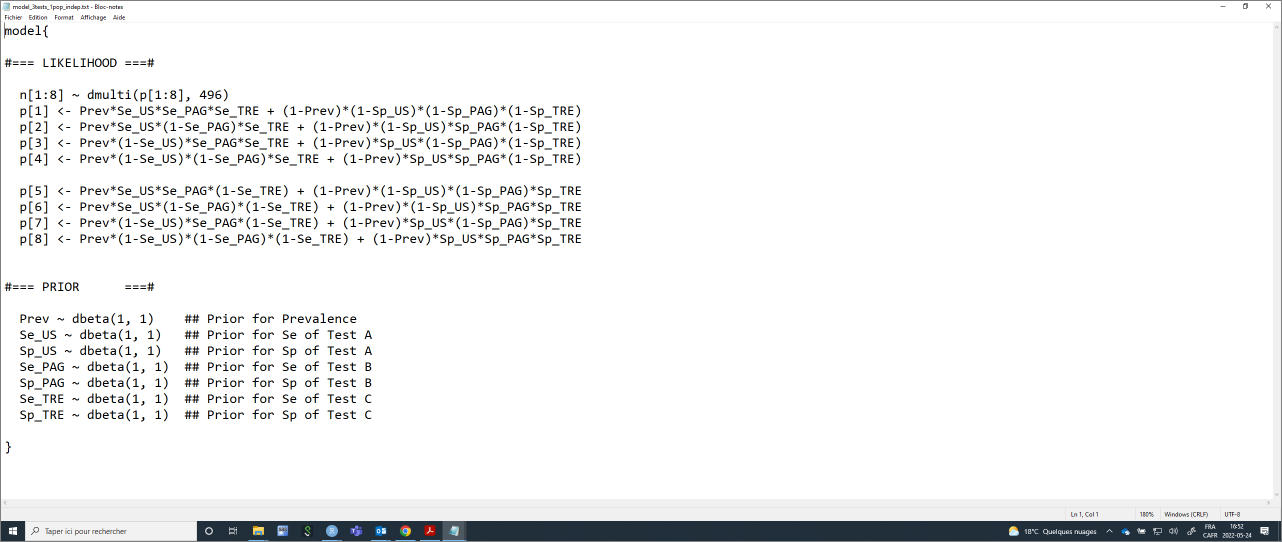
\includegraphics[keepaspectratio]{_main_files/Figures/model_3tests_1pop_indep.png}}
\caption{\textbf{Text file with the LCM for 3 independent diagnostic tests applied to one population.}}
\end{figure}

\strut \\
Again, we will need to provide a list of initial values (one per Markov chain) for all unknown parameters. Careful again, we now have three tests.

\begin{Shaded}
\begin{Highlighting}[]
\CommentTok{\#Initializing values for the parameters Prev, and the Ses and Sps of the two tests for the 3 chains.}
\NormalTok{inits }\OtherTok{\textless{}{-}} \FunctionTok{list}\NormalTok{(}\FunctionTok{list}\NormalTok{(}\AttributeTok{Prev=}\FloatTok{0.50}\NormalTok{,}
              \AttributeTok{Se\_US=}\FloatTok{0.90}\NormalTok{,}
              \AttributeTok{Sp\_US=}\FloatTok{0.90}\NormalTok{,}
              \AttributeTok{Se\_PAG=}\FloatTok{0.90}\NormalTok{,}
              \AttributeTok{Sp\_PAG=}\FloatTok{0.90}\NormalTok{,}
              \AttributeTok{Se\_TRE=}\FloatTok{0.90}\NormalTok{,}
              \AttributeTok{Sp\_TRE=}\FloatTok{0.90}\NormalTok{),}
              
              \FunctionTok{list}\NormalTok{(}\AttributeTok{Prev=}\FloatTok{0.60}\NormalTok{,}
              \AttributeTok{Se\_US=}\FloatTok{0.80}\NormalTok{,}
              \AttributeTok{Sp\_US=}\FloatTok{0.80}\NormalTok{,}
              \AttributeTok{Se\_PAG=}\FloatTok{0.80}\NormalTok{,}
              \AttributeTok{Sp\_PAG=}\FloatTok{0.80}\NormalTok{,}
              \AttributeTok{Se\_TRE=}\FloatTok{0.80}\NormalTok{,}
              \AttributeTok{Sp\_TRE=}\FloatTok{0.80}\NormalTok{),}
              
              \FunctionTok{list}\NormalTok{(}\AttributeTok{Prev=}\FloatTok{0.40}\NormalTok{,}
              \AttributeTok{Se\_US=}\FloatTok{0.70}\NormalTok{,}
              \AttributeTok{Sp\_US=}\FloatTok{0.70}\NormalTok{,}
              \AttributeTok{Se\_PAG=}\FloatTok{0.70}\NormalTok{,}
              \AttributeTok{Sp\_PAG=}\FloatTok{0.70}\NormalTok{,}
              \AttributeTok{Se\_TRE=}\FloatTok{0.70}\NormalTok{,}
              \AttributeTok{Sp\_TRE=}\FloatTok{0.70}\NormalTok{)}
\NormalTok{              )}
\end{Highlighting}
\end{Shaded}

We can run the model using \texttt{jags()} function as seen before.

\begin{Shaded}
\begin{Highlighting}[]
\FunctionTok{library}\NormalTok{(R2jags)}
\FunctionTok{library}\NormalTok{(coda)}

\CommentTok{\#Run the Bayesian model}
\NormalTok{bug.out }\OtherTok{\textless{}{-}} \FunctionTok{jags}\NormalTok{(}\AttributeTok{data=}\NormalTok{datalist,                             }
               \AttributeTok{model.file=}\StringTok{"model\_3tests\_1pop\_indep.txt"}\NormalTok{,     }
               \AttributeTok{parameters.to.save=}\FunctionTok{c}\NormalTok{(}\StringTok{"Prev"}\NormalTok{, }\StringTok{"Se\_US"}\NormalTok{, }\StringTok{"Sp\_US"}\NormalTok{, }\StringTok{"Se\_PAG"}\NormalTok{, }\StringTok{"Sp\_PAG"}\NormalTok{, }\StringTok{"Se\_TRE"}\NormalTok{, }\StringTok{"Sp\_TRE"}\NormalTok{),               }
               \AttributeTok{n.chains=}\DecValTok{3}\NormalTok{,                                 }
               \AttributeTok{inits=}\NormalTok{inits,                                }
               \AttributeTok{n.iter=}\DecValTok{11000}\NormalTok{,                                }
               \AttributeTok{n.burnin=}\DecValTok{1000}\NormalTok{,                              }
               \AttributeTok{n.thin=}\DecValTok{1}\NormalTok{,                                   }
               \AttributeTok{DIC=}\ConstantTok{FALSE}\NormalTok{)                                   }
\end{Highlighting}
\end{Shaded}

Then we could produce the diagnostic plots, compute the ESS, and print out our results as we did previously (results not shown).

\begin{Shaded}
\begin{Highlighting}[]
\FunctionTok{library}\NormalTok{(mcmcplots)}
\NormalTok{bug.mcmc }\OtherTok{\textless{}{-}} \FunctionTok{as.mcmc}\NormalTok{(bug.out)          }
\FunctionTok{mcmcplot}\NormalTok{(bug.mcmc, }\AttributeTok{title=}\StringTok{"Diagnostic plots"}\NormalTok{) }
\FunctionTok{effectiveSize}\NormalTok{(bug.mcmc)}
\FunctionTok{print}\NormalTok{(bug.out, }\AttributeTok{digits.summary=}\DecValTok{3}\NormalTok{) }
\end{Highlighting}
\end{Shaded}

\section{Conditional dependence}\label{conditional-dependence-1}

With LCM where \textgreater2 diagnostic tests are used, we could, again, relax the assumption of conditional independence by adding covariance terms representing the conditional dependence between tests \href{https://onlinelibrary.wiley.com/doi/10.1111/j.0006-341X.2001.00158.x}{(Dendukuri and Joseph, 2001)}. However, a LCM including every covariance term between every test is not always feasible. A more pragmatic approach would be to consider pair-wise covariance terms between two of the three tests.

For instance, using the example from the preceding section, we could assume that US and TRE, which are both based on recognition (tactile or visual) of the amniotic vesicle or embryo, are possibly conditionally \textbf{dependent} (as compared to the PAG test, which measure a glycoprotein associated with the placenta). We could thus include covariance terms between these two specific tests. Remember, we had set up US as Test A and TRE as Test C. It will be easier, however, to manage the covariance terms if the dependent tests are next to each other within the likelihood function. I will, therefore, re-assign the tests as follows, and reorganized the dataset with that new tests configuration.\\
-Test A: US\\
-Test B: TRE\\
-Test C: PAG

\begin{Shaded}
\begin{Highlighting}[]
\NormalTok{TestA }\OtherTok{\textless{}{-}} \StringTok{"US"}
\NormalTok{TestB }\OtherTok{\textless{}{-}} \StringTok{"TRE"}
\NormalTok{TestC }\OtherTok{\textless{}{-}} \StringTok{"PAG"}

\CommentTok{\#n is of the form : (TestA+ TestB+ Test C+), (TestA+ TestB{-} TestC+), (TestA{-} TestB+ TestC+), (TestA{-} TestB{-} TestC+), (TestA+ TestB+ Test C{-}), (TestA+ TestB{-} TestC{-}), (TestA{-} TestB+ TestC{-}), (TestA{-} TestB{-} TestC{-})}
\NormalTok{datalist }\OtherTok{\textless{}{-}} \FunctionTok{list}\NormalTok{(}\AttributeTok{n=}\FunctionTok{c}\NormalTok{(}\DecValTok{240}\NormalTok{, }\DecValTok{15}\NormalTok{, }\DecValTok{12}\NormalTok{, }\DecValTok{9}\NormalTok{, }\DecValTok{1}\NormalTok{, }\DecValTok{1}\NormalTok{, }\DecValTok{2}\NormalTok{, }\DecValTok{216}\NormalTok{))}
\NormalTok{n }\OtherTok{\textless{}{-}} \FunctionTok{sapply}\NormalTok{(datalist, sum)}

\CommentTok{\#Create the JAGS text file}
\NormalTok{model\_3tests\_1pop\_dep }\OtherTok{\textless{}{-}} \FunctionTok{paste0}\NormalTok{(}\StringTok{"model\{}

\StringTok{\#=== LIKELIHOOD ===\#}

\StringTok{  n[1:8] \textasciitilde{} dmulti(p[1:8], "}\NormalTok{,n,}\StringTok{")}
\StringTok{  p[1] \textless{}{-} Prev*(Se\_"}\NormalTok{, TestA, }\StringTok{"*Se\_"}\NormalTok{, TestB, }\StringTok{" + covp)*Se\_"}\NormalTok{, TestC, }\StringTok{" + (1{-}Prev)*((1{-}Sp\_"}\NormalTok{, TestA, }\StringTok{")*(1{-}Sp\_"}\NormalTok{, TestB, }\StringTok{") + covn)*(1{-}Sp\_"}\NormalTok{, TestC,}\StringTok{")}
\StringTok{  p[2] \textless{}{-} Prev*(Se\_"}\NormalTok{, TestA, }\StringTok{"*(1{-}Se\_"}\NormalTok{, TestB, }\StringTok{") {-} covp)*Se\_"}\NormalTok{, TestC, }\StringTok{" + (1{-}Prev)*((1{-}Sp\_"}\NormalTok{, TestA, }\StringTok{")*Sp\_"}\NormalTok{, TestB, }\StringTok{" {-} covn)*(1{-}Sp\_"}\NormalTok{, TestC,}\StringTok{")}
\StringTok{  p[3] \textless{}{-} Prev*((1{-}Se\_"}\NormalTok{, TestA, }\StringTok{")*Se\_"}\NormalTok{, TestB, }\StringTok{" {-} covp)*Se\_"}\NormalTok{, TestC, }\StringTok{" + (1{-}Prev)*(Sp\_"}\NormalTok{, TestA, }\StringTok{"*(1{-}Sp\_"}\NormalTok{, TestB, }\StringTok{") {-} covn)*(1{-}Sp\_"}\NormalTok{, TestC,}\StringTok{")}
\StringTok{  p[4] \textless{}{-} Prev*((1{-}Se\_"}\NormalTok{, TestA, }\StringTok{")*(1{-}Se\_"}\NormalTok{, TestB, }\StringTok{") + covp)*Se\_"}\NormalTok{, TestC, }\StringTok{" + (1{-}Prev)*(Sp\_"}\NormalTok{, TestA, }\StringTok{"*Sp\_"}\NormalTok{, TestB, }\StringTok{" + covn)*(1{-}Sp\_"}\NormalTok{, TestC,}\StringTok{")}
\StringTok{  }
\StringTok{  p[5] \textless{}{-} Prev*(Se\_"}\NormalTok{, TestA, }\StringTok{"*Se\_"}\NormalTok{, TestB, }\StringTok{" + covp)*(1{-}Se\_"}\NormalTok{, TestC,}\StringTok{") + (1{-}Prev)*((1{-}Sp\_"}\NormalTok{, TestA, }\StringTok{")*(1{-}Sp\_"}\NormalTok{, TestB, }\StringTok{") + covn)*Sp\_"}\NormalTok{, TestC,}\StringTok{"}
\StringTok{  p[6] \textless{}{-} Prev*(Se\_"}\NormalTok{, TestA, }\StringTok{"*(1{-}Se\_"}\NormalTok{, TestB, }\StringTok{") {-} covp)*(1{-}Se\_"}\NormalTok{, TestC,}\StringTok{") + (1{-}Prev)*((1{-}Sp\_"}\NormalTok{, TestA, }\StringTok{")*Sp\_"}\NormalTok{, TestB, }\StringTok{" {-} covn)*Sp\_"}\NormalTok{, TestC,}\StringTok{"}
\StringTok{  p[7] \textless{}{-} Prev*((1{-}Se\_"}\NormalTok{, TestA, }\StringTok{")*Se\_"}\NormalTok{, TestB, }\StringTok{" {-} covp)*(1{-}Se\_"}\NormalTok{, TestC,}\StringTok{") + (1{-}Prev)*(Sp\_"}\NormalTok{, TestA, }\StringTok{"*(1{-}Sp\_"}\NormalTok{, TestB, }\StringTok{") {-} covn)*Sp\_"}\NormalTok{, TestC,}\StringTok{"}
\StringTok{  p[8] \textless{}{-} Prev*((1{-}Se\_"}\NormalTok{, TestA, }\StringTok{")*(1{-}Se\_"}\NormalTok{, TestB, }\StringTok{") + covp)*(1{-}Se\_"}\NormalTok{, TestC,}\StringTok{") + (1{-}Prev)*(Sp\_"}\NormalTok{, TestA, }\StringTok{"*Sp\_"}\NormalTok{, TestB, }\StringTok{" + covn)*Sp\_"}\NormalTok{, TestC,}\StringTok{"}
\StringTok{  }
\StringTok{  }
\StringTok{\#=== PRIOR  ===\#}

\StringTok{  Prev \textasciitilde{} dbeta("}\NormalTok{,Prev.shapea,}\StringTok{", "}\NormalTok{,Prev.shapeb,}\StringTok{")    \#\# Prior for Prevalence}
\StringTok{  Se\_"}\NormalTok{, TestA, }\StringTok{" \textasciitilde{} dbeta("}\NormalTok{,Se.TestA.shapea,}\StringTok{", "}\NormalTok{,Se.TestA.shapeb,}\StringTok{")  \#\# Prior for Se of Test A}
\StringTok{  Sp\_"}\NormalTok{, TestA, }\StringTok{" \textasciitilde{} dbeta("}\NormalTok{,Sp.TestA.shapea,}\StringTok{", "}\NormalTok{,Sp.TestA.shapeb,}\StringTok{")  \#\# Prior for Sp of Test A}
\StringTok{  Se\_"}\NormalTok{, TestB, }\StringTok{" \textasciitilde{} dbeta("}\NormalTok{,Se.TestB.shapea,}\StringTok{", "}\NormalTok{,Se.TestB.shapeb,}\StringTok{")  \#\# Prior for Se of Test B}
\StringTok{  Sp\_"}\NormalTok{, TestB, }\StringTok{" \textasciitilde{} dbeta("}\NormalTok{,Sp.TestB.shapea,}\StringTok{", "}\NormalTok{,Sp.TestB.shapeb,}\StringTok{")  \#\# Prior for Sp of Test B}
\StringTok{  Se\_"}\NormalTok{, TestC, }\StringTok{" \textasciitilde{} dbeta("}\NormalTok{,Se.TestC.shapea,}\StringTok{", "}\NormalTok{,Se.TestC.shapeb,}\StringTok{")  \#\# Prior for Se of Test C}
\StringTok{  Sp\_"}\NormalTok{, TestC, }\StringTok{" \textasciitilde{} dbeta("}\NormalTok{,Sp.TestC.shapea,}\StringTok{", "}\NormalTok{,Sp.TestC.shapeb,}\StringTok{")  \#\# Prior for Sp of Test C}
\StringTok{  }
\StringTok{  \#=== CONDITIONAL DEPENDENCE STRUCTURE ===\#}

\StringTok{  covp \textasciitilde{} dunif(minp,maxp)}
\StringTok{  covn \textasciitilde{} dunif(minn,maxn)}
\StringTok{  minp \textless{}{-} (1{-}Se\_"}\NormalTok{, TestA, }\StringTok{")*(Se\_"}\NormalTok{, TestB, }\StringTok{"{-}1)}
\StringTok{  minn \textless{}{-} (Sp\_"}\NormalTok{, TestA, }\StringTok{"{-}1)*(1{-}Sp\_"}\NormalTok{, TestB, }\StringTok{")}
\StringTok{  maxp \textless{}{-} min(Se\_"}\NormalTok{, TestA, }\StringTok{",Se\_"}\NormalTok{, TestB, }\StringTok{") {-} Se\_"}\NormalTok{, TestA, }\StringTok{"*Se\_"}\NormalTok{, TestB, }\StringTok{"    }
\StringTok{  maxn \textless{}{-} min(Sp\_"}\NormalTok{, TestA, }\StringTok{",Sp\_"}\NormalTok{, TestB, }\StringTok{") {-} Sp\_"}\NormalTok{, TestA, }\StringTok{"*Sp\_"}\NormalTok{, TestB, }\StringTok{"  }
\StringTok{  }
\StringTok{\}"}\NormalTok{)}

\CommentTok{\#write as a text (.txt) file}
\FunctionTok{write.table}\NormalTok{(model\_3tests\_1pop\_dep, }
            \AttributeTok{file=}\StringTok{"model\_3tests\_1pop\_dep.txt"}\NormalTok{, }
            \AttributeTok{quote=}\ConstantTok{FALSE}\NormalTok{, }
            \AttributeTok{sep=}\StringTok{""}\NormalTok{, }
            \AttributeTok{row.names=}\ConstantTok{FALSE}\NormalTok{,}
            \AttributeTok{col.names=}\ConstantTok{FALSE}\NormalTok{)}
\end{Highlighting}
\end{Shaded}

The text file would look as follows:

\begin{figure}
\centering
\pandocbounded{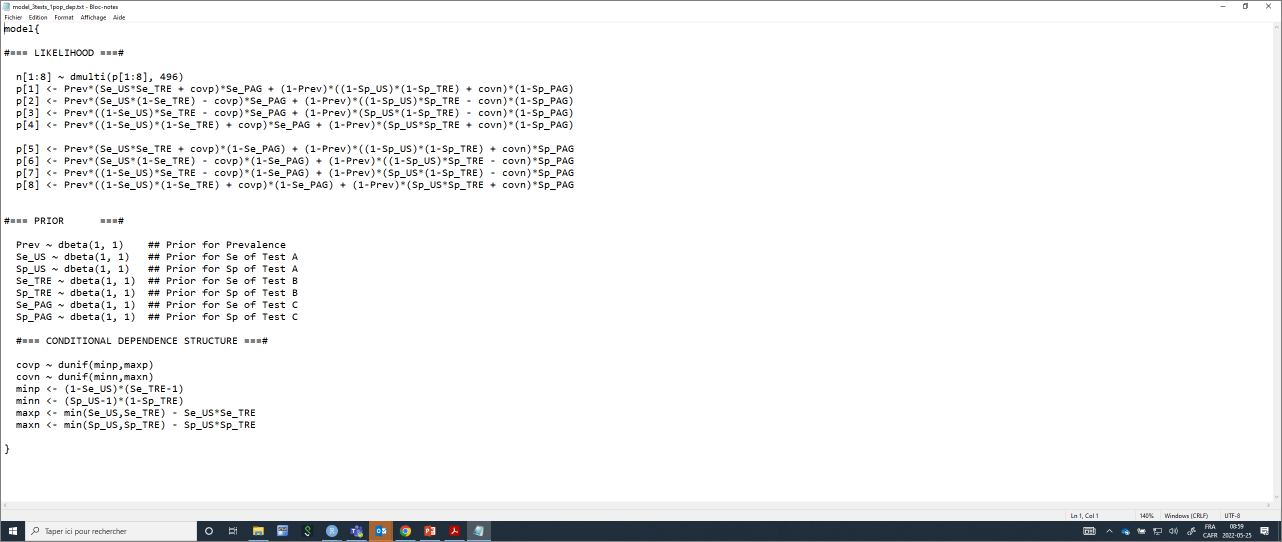
\includegraphics[keepaspectratio]{_main_files/Figures/model_3tests_1pop_dep.png}}
\caption{\textbf{Text file with the LCM for 3 diagnostic tests applied to one population and allowing for conditional dependence between two of the tests (US and TRE).}}
\end{figure}

\strut \\
We could run the model using \texttt{jags()} function and then produce the diagnostic plots, compute the ESS, and print out our results as we did previously (results not shown).

\begin{Shaded}
\begin{Highlighting}[]
\FunctionTok{library}\NormalTok{(R2jags)}
\FunctionTok{library}\NormalTok{(coda)}

\CommentTok{\#Run the Bayesian model}
\NormalTok{bug.out }\OtherTok{\textless{}{-}} \FunctionTok{jags}\NormalTok{(}\AttributeTok{data=}\NormalTok{datalist,                             }
               \AttributeTok{model.file=}\StringTok{"model\_3tests\_1pop\_dep.txt"}\NormalTok{,     }
               \AttributeTok{parameters.to.save=}\FunctionTok{c}\NormalTok{(}\StringTok{"Prev"}\NormalTok{, }\StringTok{"Se\_US"}\NormalTok{, }\StringTok{"Sp\_US"}\NormalTok{, }\StringTok{"Se\_PAG"}\NormalTok{, }\StringTok{"Sp\_PAG"}\NormalTok{, }\StringTok{"Se\_TRE"}\NormalTok{, }\StringTok{"Sp\_TRE"}\NormalTok{, }\StringTok{"covp"}\NormalTok{, }\StringTok{"covn"}\NormalTok{),               }
               \AttributeTok{n.chains=}\DecValTok{3}\NormalTok{,                                 }
               \AttributeTok{inits=}\NormalTok{inits,                                }
               \AttributeTok{n.iter=}\DecValTok{11000}\NormalTok{,                                }
               \AttributeTok{n.burnin=}\DecValTok{1000}\NormalTok{,                              }
               \AttributeTok{n.thin=}\DecValTok{1}\NormalTok{,                                   }
               \AttributeTok{DIC=}\ConstantTok{FALSE}\NormalTok{)                                   }

\FunctionTok{library}\NormalTok{(mcmcplots)}
\NormalTok{bug.mcmc }\OtherTok{\textless{}{-}} \FunctionTok{as.mcmc}\NormalTok{(bug.out)          }
\FunctionTok{mcmcplot}\NormalTok{(bug.mcmc, }\AttributeTok{title=}\StringTok{"Diagnostic plots"}\NormalTok{) }
\FunctionTok{effectiveSize}\NormalTok{(bug.mcmc)}
\FunctionTok{print}\NormalTok{(bug.out, }\AttributeTok{digits.summary=}\DecValTok{3}\NormalTok{) }
\end{Highlighting}
\end{Shaded}

In cases where you would like to consider potential conditional dependence between all tests, you could either:

\begin{itemize}
\item
  Run a number of models where you include, each time, one pairwise conditional dependence. For instance, with three tests: 1) model with \emph{TestA} \emph{vs.} \emph{TestB}; 2) model with \emph{TestA} \emph{vs.} \emph{TestC}; and 3) model with \emph{TestB} \emph{vs.} \emph{TestC}. If you are ``lucky'', perhaps just one (or none) pair of tests will yield covariance terms that are substantially different from 0.0. Then, a model with just one (or no) set of covariance terms could be used.
\item
  Include, in a single model, all potential covariance terms between 3 tests (or \textgreater{} 3 tests). For this, a different modelling approach will have to be used. As an example, \href{https://doi.org/10.3168/jds.2024-24693}{Denis-Robichaud et al.~(2024)} published a study where conditional dependence between 3 tests was allowed. The \texttt{R} script used for their analyses, along with the original dataset, was also published in this \href{https://doi.org/10.7910/DVN/EATTYD}{Dataverse}.
\end{itemize}

\chapter{Exercise 4 - Multiple tests}\label{exercise-4---multiple-tests}

\section{Questions}\label{questions-3}

Open up the \texttt{R} project for Exercise 4 (i.e., the R project file named \emph{Exercise 4.Rproj}).

In the Exercise 4 folder, you will find partially completed \texttt{R} scripts. To answer the questions, try to complete the missing parts (they are highlighted by a \textbf{\#TO COMPLETE\#} comment). We also provided complete \texttt{R} scripts, but try to work it out on your own first!

During the study comparing PAG to US, a third test (a trans-rectal manual exam; \textbf{TRE}) was conducted on most cows. To be honest, this third exam was conducted later (\textgreater50 days post-AI). But, for the sake of the exercise, you could consider that three diagnostic tests (PAG, US, and TRE) were all conducted at the same time point and develop a LCM for 3 diagnostic tests applied to one single population (i.e., herd \#1).

\textbf{Table.} Cross-classified results from a PAG, US, and TRE diagnostic tests in herd \#1.

\begin{longtable}[]{@{}ccccccc@{}}
\toprule\noalign{}
\textbf{TRE+} & & & & \textbf{TRE-} & & \\
\midrule\noalign{}
\endhead
\bottomrule\noalign{}
\endlastfoot
& \textbf{US+} & \textbf{US-} & & & \textbf{US+} & \textbf{US-} \\
\textbf{PAG+} & 126 & 3 & & \textbf{PAG+} & 12 & 7 \\
\textbf{PAG-} & 0 & 0 & & \textbf{PAG-} & 1 & 112 \\
\end{longtable}

\textbf{1.} How many degrees of freedom and unknown parameters do you have? How many informative priors will be needed?

\textbf{2. Start from the partially completed \emph{Question 2.R} script located in Exercise 4 folder.} Run a model using informative priors for US' Se and Sp and pregnancy prevalence and with vague priors on all other parameters. Then run a second model with vague priors on all parameters. We will assume conditional independence between tests and we will also assume that this is one single population. Do you expect any problems with the model using vague priors on all parameters?

\section{Answers}\label{answers-3}

\textbf{1.} How many degrees of freedom and unknown parameters do you have? How many informative priors will be needed?

\textbf{Answer:} We have 7 degrees of freedom and 7 unknown parameters, so we do not need any informative priors.

\textbf{2.} Run a model using informative priors for US and pregnancy prevalence and with vague priors on all other parameters. Then run a second model with vague priors on all parameters. We will assume conditional independence between tests and we will also assume that this is one single population. Do you expect any problem with the model using vague priors on all parameters?

\textbf{Answer:} The first model with informative priors on US' Se, Sp and on pregnancy prevalence ran well. The Markov chains were nice. With 30,000 iterations, I do get a decent ESS (around 5,000 for the worst parameter, Se\_PAG). The median estimates and 95 CI are reported in the table below.

\emph{A priori}, I would also expect that the LCM with vague priors on all parameters will work well, since it is identifiable. This was the case, the Markov chains were also nice. The lowest ESS was again around 5,000 (with 3 times 10,000 iterations). If it was for publication, we could run these LCM for more iterations to reach an ESS \textgreater{} 10,000 for all parameters. Results for the LCM with vague priors are also reported in the table below.

There were very little differences between the two LCM. Only the US' Se and Sp estimates were slightly affected. The LCM with informative priors generated posterior estimates that were somewhere in between the prior estimates and the estimates from the LCM with vague priors (i.e., between the priors and the data).

\textbf{Table.} Results from a 3 tests, 1 population LCM using different priors (informative on pregnancy prevalence and on US Se and Sp \emph{vs.} vague priors on all parameters).

\begin{longtable}[]{@{}
  >{\centering\arraybackslash}p{(\linewidth - 10\tabcolsep) * \real{0.1579}}
  >{\centering\arraybackslash}p{(\linewidth - 10\tabcolsep) * \real{0.1789}}
  >{\centering\arraybackslash}p{(\linewidth - 10\tabcolsep) * \real{0.2316}}
  >{\centering\arraybackslash}p{(\linewidth - 10\tabcolsep) * \real{0.0316}}
  >{\centering\arraybackslash}p{(\linewidth - 10\tabcolsep) * \real{0.1684}}
  >{\centering\arraybackslash}p{(\linewidth - 10\tabcolsep) * \real{0.2316}}@{}}
\toprule\noalign{}
\begin{minipage}[b]{\linewidth}\centering
\textbf{Parameter}
\end{minipage} & \begin{minipage}[b]{\linewidth}\centering
\textbf{Informative}
\end{minipage} & \begin{minipage}[b]{\linewidth}\centering
\end{minipage} & \begin{minipage}[b]{\linewidth}\centering
\end{minipage} & \begin{minipage}[b]{\linewidth}\centering
\textbf{Vague}
\end{minipage} & \begin{minipage}[b]{\linewidth}\centering
\end{minipage} \\
\midrule\noalign{}
\endhead
\bottomrule\noalign{}
\endlastfoot
& \textbf{Prior} & \textbf{Posterior} & & \textbf{Prior} & \textbf{Posterior} \\
\textbf{Prev} & Beta(4.2, 5.4) & 0.539 (0.479, 0.599) & & Beta(1.0, 1.0) & 0.541 (0.481, 0.602) \\
\textbf{Se PAG} & Beta(1.0, 1.0) & 0.995 (0.973, 1.00) & & Beta(1.0, 1.0) & 0.995 (0.972, 1.00) \\
\textbf{Sp PAG} & Beta(1.0, 1.0) & 0.942 (0.887, 0.978) & & Beta(1.0, 1.0) & 0.938 (0.885, 0.974) \\
\textbf{Se US} & Beta(100, 12) & 0.939 (0.904, 0.964) & & Beta(1.0, 1.0) & 0.972 (0.933, 0.992) \\
\textbf{Sp US} & Beta(100, 6.2) & 0.969 (0.940, 0.986) & & Beta(1.0, 1.0) & 0.986 (0.953, 0.999) \\
\textbf{Se TRE} & Beta(1.0, 1.0) & 0.907 (0.850, 0.949) & & Beta(1.0, 1.0) & 0.909 (0.852, 0.950) \\
\textbf{Sp TRE} & Beta(1.0, 1.0) & 0.994 (0.969, 1.00) & & Beta(1.0, 1.0) & 0.994 (0.967, 1.00) \\
\end{longtable}

\chapter{Accuracy varying with covariate}\label{accuracy-varying-with-covariate}

So far we have (implicitly) assumed that tests' accuracy (i.e., their Se and Sp) are the same for every individuals tested. Some diagnostic tests, however, may behave differently whether they are applied to individuals of a certain age, breed, etc. For instance, we could hypothesize that many of the diagnostic tests aiming at quantifying antibodies against a given pathogen will behave differently in neonates (which typically have an immature immune system) compared to juvenile or adult animals.

The situation where test accuracy varies as function of a characteristic of the individual tested (i.e., as function of a covariate) can be implemented relatively easily in the different LCM we have used so far. For instance, if we hypothesize that the accuracy of the PAG-based pregnancy test varies as function of whether the cow is a first lactation \emph{vs.} and older cow, we would simply specify a LCM where we have two different PAG Se and Sp, one for first lactation cows (\emph{PAG\_Se\_first} and \emph{PAG\_Sp\_first}) and one for older cows (\emph{PAG\_Se\_old} and \emph{PAG\_Sp\_old}). We would also have to provide two sets of data (one for first lactation cows and one for older cows). Of course, in that specific example, we would now have three additional unknown parameters to estimate (one additional Se, one additional Sp, and one additional prevalence), with three additional degrees of freedom (one additional 2x2 table). So investigating whether test accuracy varies as function of a covariate will not help us make the LCM identifiable. We will still need to use another trick to make the model identifiable (e.g., informative priors, \textgreater{} 1 population, or \textgreater2 diagnostic tests).

\section{Likelihood function when accuracy varies as function of covariate}\label{likelihood-function-when-accuracy-varies-as-function-of-covariate}

If we have two diagnostic tests (Test A and Test B) applied to a single population, and if we assumed that the Se and Sp of one of the test (Test A) varies as function of a characteristic (\emph{Z}) of the individual tested, then we would specify one likelihood function for the individuals without the characteristic (\emph{Z}=0) and one likelihood function for the individual having the characteristic (\emph{Z}=1). Moreover, we would estimate two Se and two Sp for the test which is hypothesized to vary as function of the covariate (\emph{Se\_Z0}, \emph{Sp\_Z0}, \emph{Se\_Z1}, \emph{Sp\_Z1}). Note that this could be extended to covariates with more than 2 levels. Thus, the likelihood function would become:

With Z=0:\\
\(n_0[1:4] \sim dmulti(P[1:4]_0, n_0)\)\\
\(P1_0 = P_0*SeA_0*SeB + (1-P_0)*(1-SpA_0)*(1-SpB)\)\\
\(P2_0 = P_0*SeA_0*(1-SeB) + (1-P_0)*(1-SpA_0)*SpB\)\\
\(P3_0 = P_0*(1-SeA_0)*SeB + (1-P_0)*SpA_0*(1-SpB)\)\\
\(P4_0 = P_0*(1-SeA_0)*(1-SeB) + (1-P_0)*SpA_0*SpB\)

With Z=1:\\
\(n_1[1:4] \sim dmulti(P[1:4]_1, n_1)\)\\
\(P1_1 = P_1*SeA_1*SeB + (1-P_1)*(1-SpA_1)*(1-SpB)\)\\
\(P2_1 = P_1*SeA_1*(1-SeB) + (1-P_1)*(1-SpA_1)*SpB\)\\
\(P3_1 = P_1*(1-SeA_1)*SeB + (1-P_1)*SpA_1*(1-SpB)\)\\
\(P4_1 = P_1*(1-SeA_1)*(1-SeB) + (1-P_1)*SpA_1*SpB\)

\section{Organizing the data when accuracy varies as function of covariate}\label{organizing-the-data-when-accuracy-varies-as-function-of-covariate}

To run such a model, we simply need to provide a dataset presenting the cross tabulated results of the two tests for individuals with \emph{Z}=0 and a second dataset for the individuals with \emph{Z}=1. For instance, in the PAG \emph{vs.} US study, the results of the PAG and US tests can be presented as function of the cow's age as follows:

\textbf{Table.} Cross-classified results from a PAG and US in first lactation \emph{vs.} older cows.

\begin{longtable}[]{@{}
  >{\centering\arraybackslash}p{(\linewidth - 12\tabcolsep) * \real{0.2394}}
  >{\centering\arraybackslash}p{(\linewidth - 12\tabcolsep) * \real{0.1268}}
  >{\centering\arraybackslash}p{(\linewidth - 12\tabcolsep) * \real{0.1268}}
  >{\centering\arraybackslash}p{(\linewidth - 12\tabcolsep) * \real{0.0423}}
  >{\centering\arraybackslash}p{(\linewidth - 12\tabcolsep) * \real{0.2113}}
  >{\centering\arraybackslash}p{(\linewidth - 12\tabcolsep) * \real{0.1268}}
  >{\centering\arraybackslash}p{(\linewidth - 12\tabcolsep) * \real{0.1268}}@{}}
\toprule\noalign{}
\begin{minipage}[b]{\linewidth}\centering
\textbf{First (Z=0)}
\end{minipage} & \begin{minipage}[b]{\linewidth}\centering
\end{minipage} & \begin{minipage}[b]{\linewidth}\centering
\end{minipage} & \begin{minipage}[b]{\linewidth}\centering
\end{minipage} & \begin{minipage}[b]{\linewidth}\centering
\textbf{Old (Z=1)}
\end{minipage} & \begin{minipage}[b]{\linewidth}\centering
\end{minipage} & \begin{minipage}[b]{\linewidth}\centering
\end{minipage} \\
\midrule\noalign{}
\endhead
\bottomrule\noalign{}
\endlastfoot
& \textbf{US+} & \textbf{US-} & & & \textbf{US+} & \textbf{US-} \\
\textbf{PAG+} & 76 & 10 & & \textbf{PAG+} & 179 & 11 \\
\textbf{PAG-} & 1 & 65 & & \textbf{PAG-} & 1 & 153 \\
\end{longtable}

The two datasets could be created as follows:

\begin{Shaded}
\begin{Highlighting}[]
\CommentTok{\#n is of the form : (TestA pos and TestB pos), (TestA pos and TestB neg), (TestA neg and TestB pos), then (TestA neg and TestB neg)}
\NormalTok{datalist }\OtherTok{\textless{}{-}} \FunctionTok{list}\NormalTok{(}\AttributeTok{Z0=}\FunctionTok{c}\NormalTok{(}\DecValTok{76}\NormalTok{,}\DecValTok{1}\NormalTok{ ,}\DecValTok{10}\NormalTok{, }\DecValTok{65}\NormalTok{),}
                 \AttributeTok{Z1=}\FunctionTok{c}\NormalTok{(}\DecValTok{179}\NormalTok{, }\DecValTok{1}\NormalTok{, }\DecValTok{11}\NormalTok{, }\DecValTok{153}\NormalTok{)}
\NormalTok{                 )}
\end{Highlighting}
\end{Shaded}

\section{The JAGS model when accuracy varies as function of covariate}\label{the-jags-model-when-accuracy-varies-as-function-of-covariate}

We could provide the values that will be used to described the prior distributions as we did before (so they are included in the model text file). The difference is that we now have, for one of the test, two Se and Sp and we also have one prevalence for \emph{Z}=0 and one prevalence for \emph{Z=1}. In the example below, I will use informative priors for these two prevalence (I will use the same priors for \emph{Z}=0 and \emph{Z}=1, but they could be different) and for US' Se and Sp.

\begin{Shaded}
\begin{Highlighting}[]
\CommentTok{\#I could first create labels for TestA and TestB}
\NormalTok{TestA }\OtherTok{\textless{}{-}} \StringTok{"US"}
\NormalTok{TestB }\OtherTok{\textless{}{-}} \StringTok{"PAG"}

\CommentTok{\#I could create labels for Z=0 and Z=1}
\NormalTok{Z0 }\OtherTok{\textless{}{-}} \StringTok{"First"}
\NormalTok{Z1 }\OtherTok{\textless{}{-}} \StringTok{"Old"}

\CommentTok{\#Provide information for the prior distributions (all beta distributions) for the unknown parameters }
\NormalTok{Prev0.shapea }\OtherTok{\textless{}{-}} \FloatTok{4.2}         \CommentTok{\#a shape parameter for Prev in Z=0    }
\NormalTok{Prev0.shapeb }\OtherTok{\textless{}{-}} \FloatTok{5.4}         \CommentTok{\#b shape parameter for Prev in Z=0}

\NormalTok{Prev1.shapea }\OtherTok{\textless{}{-}} \FloatTok{4.2}         \CommentTok{\#a shape parameter for Prev in Z=1    }
\NormalTok{Prev1.shapeb }\OtherTok{\textless{}{-}} \FloatTok{5.4}         \CommentTok{\#b shape parameter for Prev in Z=1}

\NormalTok{Se.TestA.shapea }\OtherTok{\textless{}{-}} \DecValTok{131}     \CommentTok{\#a shape parameter for Se of TestA}
\NormalTok{Se.TestA.shapeb }\OtherTok{\textless{}{-}} \DecValTok{15}     \CommentTok{\#b shape parameter for Se of TestA}
\NormalTok{Sp.TestA.shapea }\OtherTok{\textless{}{-}} \DecValTok{100}     \CommentTok{\#a shape parameter for Sp of TestA}
\NormalTok{Sp.TestA.shapeb }\OtherTok{\textless{}{-}} \DecValTok{6}     \CommentTok{\#b shape parameter for Sp of TestA}

\NormalTok{Se.TestB.Z0.shapea }\OtherTok{\textless{}{-}} \DecValTok{1}     \CommentTok{\#a shape parameter for Se of TestB in Z=0}
\NormalTok{Se.TestB.Z0.shapeb }\OtherTok{\textless{}{-}} \DecValTok{1}     \CommentTok{\#b shape parameter for Se of TestB in Z=0}
\NormalTok{Sp.TestB.Z0.shapea }\OtherTok{\textless{}{-}} \DecValTok{1}     \CommentTok{\#a shape parameter for Sp of TestB in Z=0}
\NormalTok{Sp.TestB.Z0.shapeb }\OtherTok{\textless{}{-}} \DecValTok{1}     \CommentTok{\#b shape parameter for Sp of TestB in Z=0}

\NormalTok{Se.TestB.Z1.shapea }\OtherTok{\textless{}{-}} \DecValTok{1}     \CommentTok{\#a shape parameter for Se of TestB in Z=1}
\NormalTok{Se.TestB.Z1.shapeb }\OtherTok{\textless{}{-}} \DecValTok{1}     \CommentTok{\#b shape parameter for Se of TestB in Z=1}
\NormalTok{Sp.TestB.Z1.shapea }\OtherTok{\textless{}{-}} \DecValTok{1}     \CommentTok{\#a shape parameter for Sp of TestB in Z=1}
\NormalTok{Sp.TestB.Z1.shapeb }\OtherTok{\textless{}{-}} \DecValTok{1}     \CommentTok{\#b shape parameter for Sp of TestB in Z=1}

\CommentTok{\#I will also need the number of individuals tested in each populations (n0 and n1)}
\NormalTok{n }\OtherTok{\textless{}{-}} \FunctionTok{sapply}\NormalTok{(datalist, sum)}
\NormalTok{n0 }\OtherTok{\textless{}{-}}\NormalTok{ n[}\DecValTok{1}\NormalTok{]}
\NormalTok{n1 }\OtherTok{\textless{}{-}}\NormalTok{ n[}\DecValTok{2}\NormalTok{]}
\end{Highlighting}
\end{Shaded}

With that, we have everything that is needed to write the JAGS model.

\begin{Shaded}
\begin{Highlighting}[]
\CommentTok{\#Create the JAGS text file}
\NormalTok{model\_2tests\_covariate }\OtherTok{\textless{}{-}} \FunctionTok{paste0}\NormalTok{(}\StringTok{"model\{}

\StringTok{\#=== LIKELIHOOD ===\#}
\StringTok{  \#For Z=0}
\StringTok{  Z0[1:4] \textasciitilde{} dmulti(p0[1:4], "}\NormalTok{,n0,}\StringTok{")}
\StringTok{  p0[1] \textless{}{-} Prev\_"}\NormalTok{, Z0,}\StringTok{"*Se\_"}\NormalTok{, TestA, }\StringTok{"*Se\_"}\NormalTok{, TestB, }\StringTok{"\_"}\NormalTok{, Z0,}\StringTok{" + (1{-}Prev\_"}\NormalTok{, Z0,}\StringTok{")*(1{-}Sp\_"}\NormalTok{, TestA, }\StringTok{")*(1{-}Sp\_"}\NormalTok{, TestB, }\StringTok{"\_"}\NormalTok{, Z0,}\StringTok{")}
\StringTok{  p0[2] \textless{}{-} Prev\_"}\NormalTok{, Z0,}\StringTok{"*Se\_"}\NormalTok{, TestA, }\StringTok{"*(1{-}Se\_"}\NormalTok{, TestB, }\StringTok{"\_"}\NormalTok{, Z0,}\StringTok{") + (1{-}Prev\_"}\NormalTok{, Z0,}\StringTok{")*(1{-}Sp\_"}\NormalTok{, TestA, }\StringTok{")*Sp\_"}\NormalTok{, TestB, }\StringTok{"\_"}\NormalTok{, Z0,}\StringTok{"}
\StringTok{  p0[3] \textless{}{-} Prev\_"}\NormalTok{, Z0,}\StringTok{"*(1{-}Se\_"}\NormalTok{, TestA, }\StringTok{")*Se\_"}\NormalTok{, TestB, }\StringTok{"\_"}\NormalTok{, Z0,}\StringTok{" + (1{-}Prev\_"}\NormalTok{, Z0,}\StringTok{")*Sp\_"}\NormalTok{, TestA, }\StringTok{"*(1{-}Sp\_"}\NormalTok{, TestB, }\StringTok{"\_"}\NormalTok{, Z0,}\StringTok{")}
\StringTok{  p0[4] \textless{}{-} Prev\_"}\NormalTok{, Z0,}\StringTok{"*(1{-}Se\_"}\NormalTok{, TestA, }\StringTok{")*(1{-}Se\_"}\NormalTok{, TestB, }\StringTok{"\_"}\NormalTok{, Z0,}\StringTok{") + (1{-}Prev\_"}\NormalTok{, Z0,}\StringTok{")*Sp\_"}\NormalTok{, TestA, }\StringTok{"*Sp\_"}\NormalTok{, TestB, }\StringTok{"\_"}\NormalTok{, Z0,}\StringTok{"}
\StringTok{  }
\StringTok{  \#For Z=1}
\StringTok{  Z1[1:4] \textasciitilde{} dmulti(p1[1:4], "}\NormalTok{,n1,}\StringTok{")}
\StringTok{  p1[1] \textless{}{-} Prev\_"}\NormalTok{, Z1,}\StringTok{"*Se\_"}\NormalTok{, TestA, }\StringTok{"*Se\_"}\NormalTok{, TestB, }\StringTok{"\_"}\NormalTok{, Z1,}\StringTok{" + (1{-}Prev\_"}\NormalTok{, Z1,}\StringTok{")*(1{-}Sp\_"}\NormalTok{, TestA, }\StringTok{")*(1{-}Sp\_"}\NormalTok{, TestB, }\StringTok{"\_"}\NormalTok{, Z1,}\StringTok{")}
\StringTok{  p1[2] \textless{}{-} Prev\_"}\NormalTok{, Z1,}\StringTok{"*Se\_"}\NormalTok{, TestA, }\StringTok{"*(1{-}Se\_"}\NormalTok{, TestB, }\StringTok{"\_"}\NormalTok{, Z1,}\StringTok{") + (1{-}Prev\_"}\NormalTok{, Z1,}\StringTok{")*(1{-}Sp\_"}\NormalTok{, TestA, }\StringTok{")*Sp\_"}\NormalTok{, TestB, }\StringTok{"\_"}\NormalTok{, Z1,}\StringTok{"}
\StringTok{  p1[3] \textless{}{-} Prev\_"}\NormalTok{, Z1,}\StringTok{"*(1{-}Se\_"}\NormalTok{, TestA, }\StringTok{")*Se\_"}\NormalTok{, TestB, }\StringTok{"\_"}\NormalTok{, Z1,}\StringTok{" + (1{-}Prev\_"}\NormalTok{, Z1,}\StringTok{")*Sp\_"}\NormalTok{, TestA, }\StringTok{"*(1{-}Sp\_"}\NormalTok{, TestB, }\StringTok{"\_"}\NormalTok{, Z1,}\StringTok{")}
\StringTok{  p1[4] \textless{}{-} Prev\_"}\NormalTok{, Z1,}\StringTok{"*(1{-}Se\_"}\NormalTok{, TestA, }\StringTok{")*(1{-}Se\_"}\NormalTok{, TestB, }\StringTok{"\_"}\NormalTok{, Z1,}\StringTok{") + (1{-}Prev\_"}\NormalTok{, Z1,}\StringTok{")*Sp\_"}\NormalTok{, TestA, }\StringTok{"*Sp\_"}\NormalTok{, TestB, }\StringTok{"\_"}\NormalTok{, Z1,}\StringTok{"}
\StringTok{   }

\StringTok{\#=== PRIOR  ===\#}

\StringTok{  Prev\_"}\NormalTok{, Z0,}\StringTok{" \textasciitilde{} dbeta("}\NormalTok{,Prev0.shapea,}\StringTok{", "}\NormalTok{,Prev0.shapeb,}\StringTok{")  \#\# Prior for Prev in Z=0}
\StringTok{  Prev\_"}\NormalTok{, Z1,}\StringTok{" \textasciitilde{} dbeta("}\NormalTok{,Prev1.shapea,}\StringTok{", "}\NormalTok{,Prev1.shapeb,}\StringTok{")  \#\# Prior for Prev in Z=1}
\StringTok{  Se\_"}\NormalTok{, TestA, }\StringTok{" \textasciitilde{} dbeta("}\NormalTok{,Se.TestA.shapea,}\StringTok{", "}\NormalTok{,Se.TestA.shapeb,}\StringTok{")  \#\# Prior for Se of Test A}
\StringTok{  Sp\_"}\NormalTok{, TestA, }\StringTok{" \textasciitilde{} dbeta("}\NormalTok{,Sp.TestA.shapea,}\StringTok{", "}\NormalTok{,Sp.TestA.shapeb,}\StringTok{")  \#\# Prior for Sp of Test A}
\StringTok{  Se\_"}\NormalTok{, TestB, }\StringTok{"\_"}\NormalTok{, Z0, }\StringTok{" \textasciitilde{} dbeta("}\NormalTok{,Se.TestB.Z0.shapea,}\StringTok{", "}\NormalTok{,Se.TestB.Z0.shapeb,}\StringTok{")   \#\# Prior for Se of Test B in Z=0}
\StringTok{  Sp\_"}\NormalTok{, TestB, }\StringTok{"\_"}\NormalTok{, Z0, }\StringTok{" \textasciitilde{} dbeta("}\NormalTok{,Sp.TestB.Z0.shapea,}\StringTok{", "}\NormalTok{,Sp.TestB.Z0.shapeb,}\StringTok{")   \#\# Prior for Sp of Test B in Z=0}
\StringTok{  Se\_"}\NormalTok{, TestB, }\StringTok{"\_"}\NormalTok{, Z1, }\StringTok{" \textasciitilde{} dbeta("}\NormalTok{,Se.TestB.Z1.shapea,}\StringTok{", "}\NormalTok{,Se.TestB.Z1.shapeb,}\StringTok{")   \#\# Prior for Se of Test B in Z=1}
\StringTok{  Sp\_"}\NormalTok{, TestB, }\StringTok{"\_"}\NormalTok{, Z1, }\StringTok{" \textasciitilde{} dbeta("}\NormalTok{,Sp.TestB.Z1.shapea,}\StringTok{", "}\NormalTok{,Sp.TestB.Z1.shapeb,}\StringTok{")   \#\# Prior for Sp of Test B in Z=1}
\StringTok{  }
\StringTok{\}"}\NormalTok{)}

\CommentTok{\#write as a text (.txt) file}
\FunctionTok{write.table}\NormalTok{(model\_2tests\_covariate, }
            \AttributeTok{file=}\StringTok{"model\_2tests\_covariate.txt"}\NormalTok{, }
            \AttributeTok{quote=}\ConstantTok{FALSE}\NormalTok{, }
            \AttributeTok{sep=}\StringTok{""}\NormalTok{, }
            \AttributeTok{row.names=}\ConstantTok{FALSE}\NormalTok{,}
            \AttributeTok{col.names=}\ConstantTok{FALSE}\NormalTok{)}
\end{Highlighting}
\end{Shaded}

With this code, you could, again, simply modify the labels for Test A and Test B, and for Z0 and Z1, and the shape parameters for the prior distributions. The text file with the JAGS model will automatically be updated. Currently, it looks like this:

\begin{figure}
\centering
\pandocbounded{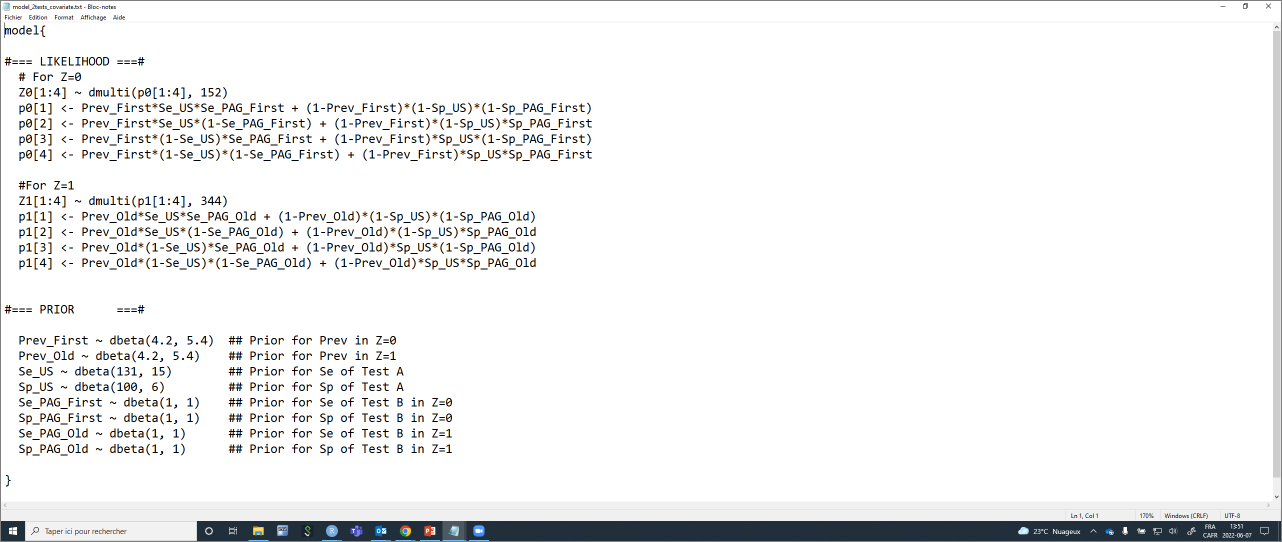
\includegraphics[keepaspectratio]{_main_files/Figures/model_2tests_covariate.png}}
\caption{\textbf{Text file with the LCM for 2 independent diagnostic tests applied to one population but with one of the test accuracy varying as function of a covariate.}}
\end{figure}

\strut \\
Again, we will need to provide a list of initial values (one per Markov chain) for all unknown parameters. Careful, we now have two tests, but two Se and Sp for one of the test, and two prevalence.

\begin{Shaded}
\begin{Highlighting}[]
\CommentTok{\#Initializing values for the parameters Prev, and the Ses and Sps of the two tests for the 3 chains.}
\NormalTok{inits }\OtherTok{\textless{}{-}} \FunctionTok{list}\NormalTok{(}\FunctionTok{list}\NormalTok{(}\AttributeTok{Prev\_First=}\FloatTok{0.50}\NormalTok{,}
              \AttributeTok{Prev\_Old=}\FloatTok{0.50}\NormalTok{,}
              \AttributeTok{Se\_US=}\FloatTok{0.90}\NormalTok{,}
              \AttributeTok{Sp\_US=}\FloatTok{0.90}\NormalTok{,}
              \AttributeTok{Se\_PAG\_First=}\FloatTok{0.90}\NormalTok{,}
              \AttributeTok{Sp\_PAG\_First=}\FloatTok{0.90}\NormalTok{,}
              \AttributeTok{Se\_PAG\_Old=}\FloatTok{0.90}\NormalTok{,}
              \AttributeTok{Sp\_PAG\_Old=}\FloatTok{0.90}\NormalTok{),}
              
              \FunctionTok{list}\NormalTok{(}\AttributeTok{Prev\_First=}\FloatTok{0.60}\NormalTok{,}
              \AttributeTok{Prev\_Old=}\FloatTok{0.60}\NormalTok{,}
              \AttributeTok{Se\_US=}\FloatTok{0.80}\NormalTok{,}
              \AttributeTok{Sp\_US=}\FloatTok{0.80}\NormalTok{,}
              \AttributeTok{Se\_PAG\_First=}\FloatTok{0.80}\NormalTok{,}
              \AttributeTok{Sp\_PAG\_First=}\FloatTok{0.80}\NormalTok{,}
              \AttributeTok{Se\_PAG\_Old=}\FloatTok{0.80}\NormalTok{,}
              \AttributeTok{Sp\_PAG\_Old=}\FloatTok{0.80}\NormalTok{),}
              
              \FunctionTok{list}\NormalTok{(}\AttributeTok{Prev\_First=}\FloatTok{0.40}\NormalTok{,}
              \AttributeTok{Prev\_Old=}\FloatTok{0.40}\NormalTok{,}
              \AttributeTok{Se\_US=}\FloatTok{0.70}\NormalTok{,}
              \AttributeTok{Sp\_US=}\FloatTok{0.70}\NormalTok{,}
              \AttributeTok{Se\_PAG\_First=}\FloatTok{0.70}\NormalTok{,}
              \AttributeTok{Sp\_PAG\_First=}\FloatTok{0.70}\NormalTok{,}
              \AttributeTok{Se\_PAG\_Old=}\FloatTok{0.70}\NormalTok{,}
              \AttributeTok{Sp\_PAG\_Old=}\FloatTok{0.70}\NormalTok{)}
\NormalTok{              )}
\end{Highlighting}
\end{Shaded}

We can run the model using \texttt{jags()} function as seen before.

\begin{Shaded}
\begin{Highlighting}[]
\FunctionTok{library}\NormalTok{(R2jags)}
\FunctionTok{library}\NormalTok{(coda)}

\CommentTok{\#Run the Bayesian model}
\NormalTok{bug.out }\OtherTok{\textless{}{-}} \FunctionTok{jags}\NormalTok{(}\AttributeTok{data=}\NormalTok{datalist,                             }
               \AttributeTok{model.file=}\StringTok{"model\_2tests\_covariate.txt"}\NormalTok{,     }
               \AttributeTok{parameters.to.save=}\FunctionTok{c}\NormalTok{(}\StringTok{"Prev\_First"}\NormalTok{, }\StringTok{"Prev\_Old"}\NormalTok{,}\StringTok{"Se\_US"}\NormalTok{, }\StringTok{"Sp\_US"}\NormalTok{, }\StringTok{"Se\_PAG\_First"}\NormalTok{, }\StringTok{"Sp\_PAG\_First"}\NormalTok{, }\StringTok{"Se\_PAG\_Old"}\NormalTok{, }\StringTok{"Sp\_PAG\_Old"}\NormalTok{),               }
               \AttributeTok{n.chains=}\DecValTok{3}\NormalTok{,                                 }
               \AttributeTok{inits=}\NormalTok{inits,                                }
               \AttributeTok{n.iter=}\DecValTok{11000}\NormalTok{,                                }
               \AttributeTok{n.burnin=}\DecValTok{1000}\NormalTok{,                              }
               \AttributeTok{n.thin=}\DecValTok{1}\NormalTok{,                                   }
               \AttributeTok{DIC=}\ConstantTok{FALSE}\NormalTok{)                                   }
\end{Highlighting}
\end{Shaded}

Then we could produce the diagnostic plots, compute the ESS, and print out our results as we did previously (results not shown).

\begin{Shaded}
\begin{Highlighting}[]
\FunctionTok{library}\NormalTok{(mcmcplots)}
\NormalTok{bug.mcmc }\OtherTok{\textless{}{-}} \FunctionTok{as.mcmc}\NormalTok{(bug.out)          }
\FunctionTok{mcmcplot}\NormalTok{(bug.mcmc, }\AttributeTok{title=}\StringTok{"Diagnostic plots"}\NormalTok{) }
\FunctionTok{effectiveSize}\NormalTok{(bug.mcmc)}
\FunctionTok{print}\NormalTok{(bug.out, }\AttributeTok{digits.summary=}\DecValTok{3}\NormalTok{) }
\end{Highlighting}
\end{Shaded}

\chapter{Exercise 5 - Accuracy varying with covariate}\label{exercise-5---accuracy-varying-with-covariate}

\section{Questions}\label{questions-4}

Open up the \texttt{R} project for Exercise 5 (i.e., the R project file named \emph{Exercise 5.Rproj}).

In the Exercise 5 folder, you will find partially completed \texttt{R} scripts. To answer the questions, try to complete the missing parts (they are highlighted by a \textbf{\#TO COMPLETE\#} comment). We also provided complete \texttt{R} scripts, but try to work it out on your own first!

Some anecdotic reports suggest that expression of PAG may vary as function of number of days of pregnancy. We could, therefore, hypothesize that PAG's Se and Sp may vary if the test is conducted early (≤ 35 days post-breeding) compared to later (\textgreater35 days post-breeding). When cross-tabulating the studies results for the PAG and US tests as function of days since breeding, we get:

\textbf{Table.} Cross-classified results from a PAG and US test as function of number of days since breeding.

\begin{longtable}[]{@{}
  >{\centering\arraybackslash}p{(\linewidth - 12\tabcolsep) * \real{0.2206}}
  >{\centering\arraybackslash}p{(\linewidth - 12\tabcolsep) * \real{0.1324}}
  >{\centering\arraybackslash}p{(\linewidth - 12\tabcolsep) * \real{0.1324}}
  >{\centering\arraybackslash}p{(\linewidth - 12\tabcolsep) * \real{0.0441}}
  >{\centering\arraybackslash}p{(\linewidth - 12\tabcolsep) * \real{0.2059}}
  >{\centering\arraybackslash}p{(\linewidth - 12\tabcolsep) * \real{0.1324}}
  >{\centering\arraybackslash}p{(\linewidth - 12\tabcolsep) * \real{0.1324}}@{}}
\toprule\noalign{}
\begin{minipage}[b]{\linewidth}\centering
\textbf{≤ 35 days}
\end{minipage} & \begin{minipage}[b]{\linewidth}\centering
\end{minipage} & \begin{minipage}[b]{\linewidth}\centering
\end{minipage} & \begin{minipage}[b]{\linewidth}\centering
\end{minipage} & \begin{minipage}[b]{\linewidth}\centering
\textbf{\textgreater35 days}
\end{minipage} & \begin{minipage}[b]{\linewidth}\centering
\end{minipage} & \begin{minipage}[b]{\linewidth}\centering
\end{minipage} \\
\midrule\noalign{}
\endhead
\bottomrule\noalign{}
\endlastfoot
& \textbf{US+} & \textbf{US-} & & & \textbf{US+} & \textbf{US-} \\
\textbf{PAG+} & 143 & 11 & & \textbf{PAG+} & 112 & 10 \\
\textbf{PAG-} & 2 & 136 & & \textbf{PAG-} & 0 & 82 \\
\end{longtable}

\textbf{1.Start from the partially completed \emph{Question 1.R} script located in Exercise 5 folder.} Build a model for two diagnostic tests, one single population, but with Se and Sp of the PAG test varying as function of days since breeding. Use the \href{https://www.sciencedirect.com/science/article/pii/S0093691X06001543?via\%3Dihub}{Romano et al.~(2006)} results, to inform the priors for the Se and Sp of a US exam (Se: 0.90, 95CI: 0.85, 0.95; Sp: 0.95, 95CI: 0.90, 0.97). Assume conditional independence between tests. How many degrees of freedom do you have and how many unknown parameters do you need to estimate? Based on your results, would you conclude that PAG accuracy is influenced by number of days since breeding?

\section{Answers}\label{answers-4}

\textbf{1.} How many degrees of freedom do you have and how many unknown parameters do you need to estimate? Based on your results, would you conclude that PAG accuracy is influenced by number of days since breeding?

\textbf{Answer:} We have 6 degrees of freedom and 8 unknown parameters to estimate (one Se and one Sp for US, 2 Se and 2 Sp for PAG, and two prevalence). We need two informative priors to make the LCM identifiable.

The results from this LCM are below.

\textbf{Table.} Results for the LCM allowing for varying accuracy of PAG as function of days since breeding.

\begin{longtable}[]{@{}ccc@{}}
\toprule\noalign{}
\textbf{Parameter} & \textbf{Median} & \textbf{95CI} \\
\midrule\noalign{}
\endhead
\bottomrule\noalign{}
\endlastfoot
\textbf{Prevalence 28-35 days} & 0.521 & 0.462, 0.580 \\
\textbf{Prevalence 36-45 days} & 0.584 & 0.512, 0.653 \\
\textbf{Se US} & 0.928 & 0.895, 0.956 \\
\textbf{Sp US} & 0.977 & 0.957, 0.990 \\
\textbf{Se PAG 28-35 days} & 0.991 & 0.963, 1.00 \\
\textbf{Se PAG 36-45 days} & 0.994 & 0.966, 1.00 \\
\textbf{Sp PAG 28-35 days} & 0.980 & 0.927, 0.999 \\
\textbf{Sp PAG 36-45 days} & 0.962 & 0.879, 0.998 \\
\end{longtable}

There was little difference between the 28-35 days since breeding \emph{vs.} 36-45 days since breeding accuracy parameters. Below, we have plotted the two PAG Sp posterior distributions to illustrate how similar they are. However, since we are not in a Frequentist framework, ``testing'' whether the 28-35 days \emph{vs.} 36-45 days accuracy parameters are statistically different is not straightforward. Note that Bayesian methods can be used to compute the probability that a given parameter is larger (or smaller) than another parameter, or than an estimate previously reported in the literature \href{https://doi.org/10.1016/j.prevetmed.2021.105510}{(see Arango-Sabogal et al., 2021} for an applied example.

\begin{figure}
\centering
\pandocbounded{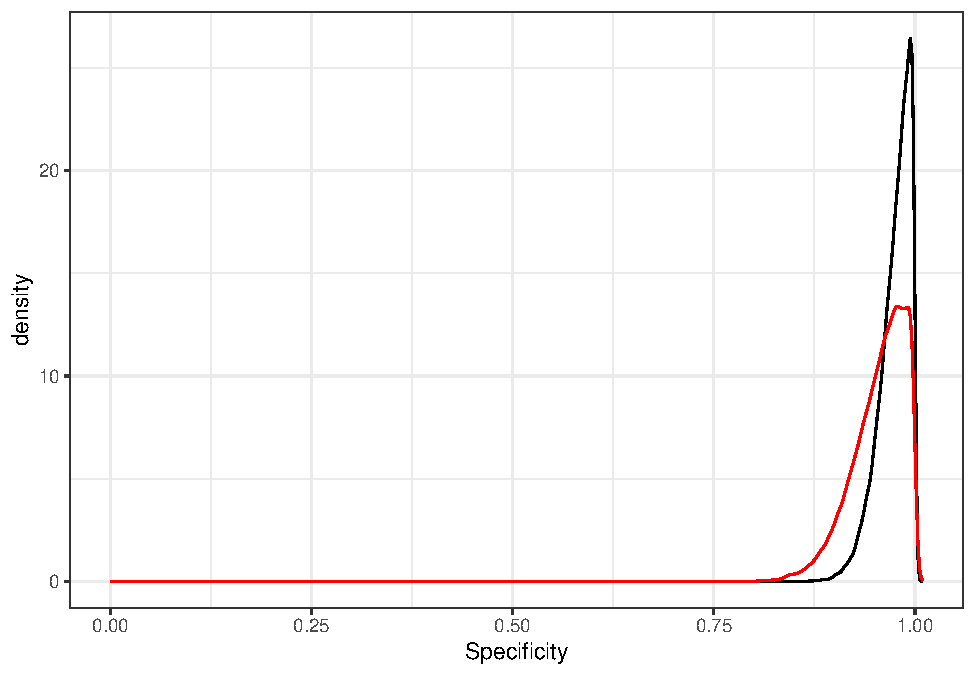
\includegraphics[keepaspectratio]{_main_files/_main_files/figure-latex/unnamed-chunk-91-1.pdf}}
\caption{\label{fig:unnamed-chunk-91}Posterior distributions for PAG specificity at 28-35 days (black) and 36-45 days (red) post-breeding.}
\end{figure}

\chapter{Extensions}\label{extensions-1}

In this document we have described some of the ``main'' LCM. More specifically we described LCMs that can be used with:

-\textbf{Two} conditionally \textbf{independent} diagnostic tests applied in \textbf{one single population};\\
-\textbf{Two} conditionally \textbf{dependent} diagnostic tests applied in \textbf{one single population};\\
-\textbf{Two} conditionally \textbf{independent} diagnostic tests applied in \textbf{more than one population} (using a conventional or hierarchical model);\\
-\textbf{Two} conditionally \textbf{dependent} diagnostic tests applied in \textbf{more than one population} (using a conventional or hierarchical model);\\
-\textbf{More than two} conditionally \textbf{independent} diagnostic tests applied in \textbf{one single population};\\
-\textbf{More than two} diagnostic tests applied in \textbf{one single population} and with conditional \textbf{dependence} between two of the tests;\\
-\textbf{Two} conditionally \textbf{independent} diagnostic tests, but with \textbf{accuracy of one or both tests varying as function of a characteristic of the individual tested};

From here, it is up to you to adapt these LCMs to fit your needs. For instance, you could have a study where three tests were applied to one population, but two of these tests were also applied to a second population. For two of the tests, you may want to relax the assumption of conditional dependence by including covariance terms between them. Finally, you may want to allow the Se and Sp of one of the test to vary as function of a characteristic of the individual tested.

When working with a ``customized'' LCM, the principles that we have discussed still apply. It will always be a good starting point to:

-Count the number of unknown parameters to estimate;\\
-Organize the dataset(s);\\
-Evaluate whether some tests combinations are not observed;\\
-Count the number of degrees of freedom available;\\
-Identify the number of informative priors that will be needed;\\
-Consider whether scientific literature will be available to develop the needed informative priors;

Based on this initial assessment, you will be able to decide whether running this LCM is doable, or if it would be better to revise your plans.

\chapter{Sensitivity analyses}\label{sensitivity-analyses}

An important step of any Bayesian analysis is to evaluate whether the results are strongly affected by the model's assumptions and/or the choice of priors.

\section{Model's assumptions}\label{models-assumptions}

Regarding the sensitivity of our results to the assumptions made, this could be assessed by comparing the results from the LCM where a given assumption was made \emph{vs.} the ones from a LCM where the assumption was relaxed. Of course, \textbf{to fully ``isolate'' the effect of a given assumption, the same priors would have to be used in both LCM}. This is, however, not always possible since, sometimes, the ``relaxed'' LCM may require a larger number of informative priors to make it identifiable.

In the end, providing the results from an ``alternative'' LCM could help the readers understand what was the influence of the model chosen on the presented results. As author, you would probably want to use the LCM that is the most ``biologically relevant'' as your main model, but present the results of these alternative models to illustrate how the choice of model may have impacted the results.

Below are some of the main assumptions that you may want to evaluate.

\subsection{Conditional independence between tests}\label{conditional-independence-between-tests}

Even if two tests rely on very different biological processes, it would be a good practice to evaluate whether allowing for conditional dependence between tests would produce different results. You could do this using the model described in Chapter 5.

\subsection{Constant test accuracy across populations}\label{constant-test-accuracy-across-populations}

To evaluate whether test's accuracy is constant across populations, the following options could be used:

\begin{itemize}
\tightlist
\item
  Check if the accuracy vary as function of a characteristic of the tested individuals (e.g., age, breed, etc);\\
\item
  If a substantial number of populations were studied:

  \begin{itemize}
  \tightlist
  \item
    We could run the model after removing one of the population and repeat this process for each population. If the results (e.g., the test's accuracy parameters) differ substantially for one of the model, this could indicate that the test accuracy is different in this population;\\
  \item
    We could allow for different accuracy in one or many of the populations. For instance, we may define \emph{TestA} accuracy as \emph{SeA-2} and \emph{SpA-2} in one (or some) of the populations studied and as \emph{SeA} and \emph{SpA} for all other populations. If the \emph{SeA} and \emph{SeA-2} (or \emph{SpA} and \emph{SpA-2}) parameters differ substantially, this may, again, indicate that the test accuracy is different in this population.
  \end{itemize}
\end{itemize}

\subsection{Prevalence varies from one population to another}\label{prevalence-varies-from-one-population-to-another}

This latter assumption is important for the \href{https://www.jstor.org/stable/2530508?seq=1}{Hui and Walter (1980)} model and other similar models. One thing that can be done is to ``eyeball'' the initial tests' results and/or the estimated prevalence to confirm some differences between populations in, respectively, the apparent and/or true prevalence.

Besides, \href{https://projecteuclid.org/journals/statistical-science/volume-20/issue-2/On-Model-Expansion-Model-Contraction-Identifiability-and-Prior-Information/10.1214/088342305000000098.full}{Gustafson et al.~(2005)} have reviewed the impacts of having two populations with very similar prevalence and the only impact was a lack of identifiability of the model. This latter issue would results in non-converging Markov chains for one or a few of the unknown parameters. If the Markov chains converged, then the assumption of varying prevalence between population is probably not a problem.

\section{Choice of priors}\label{choice-of-priors}

Whenever informative priors are used in a LCM, the sensitivity of the LCM to the choice of priors should be assessed. This can be done by running the same LCM, but with ``perturbed'' and usually ``more diffuse'' priors. \href{https://doi.org/10.1016/j.prevetmed.2019.01.010}{Johnson et al.~(2019)} recommended, for instance, to move the mode of the prior distribution of a given parameter by a few percentage-points (e.g., -15 percentage-points) and to increase the width of its prior distribution. Then, the results from the LCM using the scientific literature-derived priors can be compared to those of the LCM using perturbed priors to assess how sensitive to the choice of priors the results are. The amount and direction by which the mode will be moved and the level of increase of the width of the distribution will depend on the problem at hand.

For instance, in the preceding sections we used the \href{https://www.sciencedirect.com/science/article/pii/S0093691X06001543?via\%3Dihub}{Romano et al.~(2006)} results, to inform the priors for the Se and Sp of a US exam conducted between 28-45 days post-insemination:\\
-Se = 0.90 (95CI: 0.85, 0.95)\\
-Sp = 0.95 (95CI: 0.90, 0.97)

We thus came up with these prior distributions for US' Se and sp.

\pandocbounded{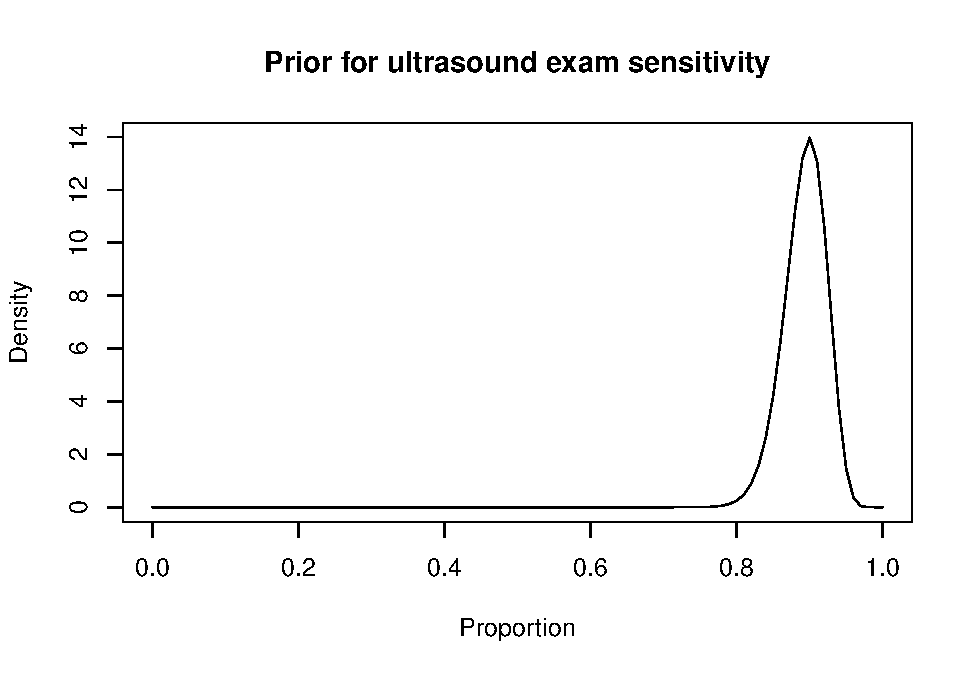
\includegraphics[keepaspectratio]{_main_files/_main_files/figure-latex/unnamed-chunk-94-1.pdf}}

\pandocbounded{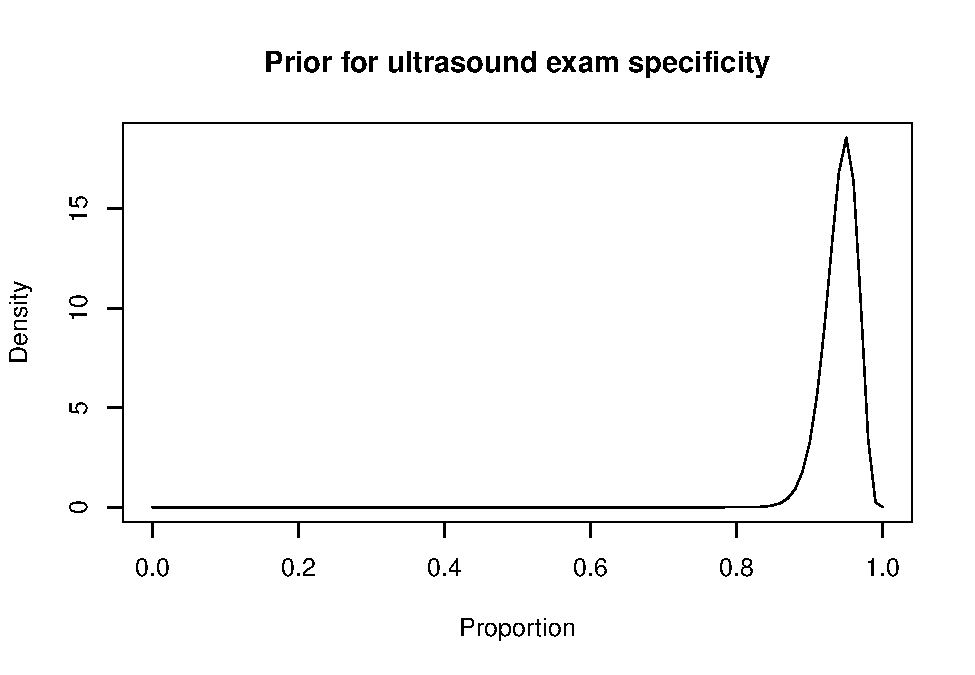
\includegraphics[keepaspectratio]{_main_files/_main_files/figure-latex/unnamed-chunk-95-1.pdf}}

Thus, a possibility could be to move down the Se and Sp modes by 10 percentage points (i.e., mode for Se: 0.80 and mode for Sp: 0.85) and to increase the width of the distribution by moving the 2.5th percentiles by 30 percentage-points (Se 2.5th percentile: 0.55; Sp 2.5th percentile: 0.60). Thus:

\pandocbounded{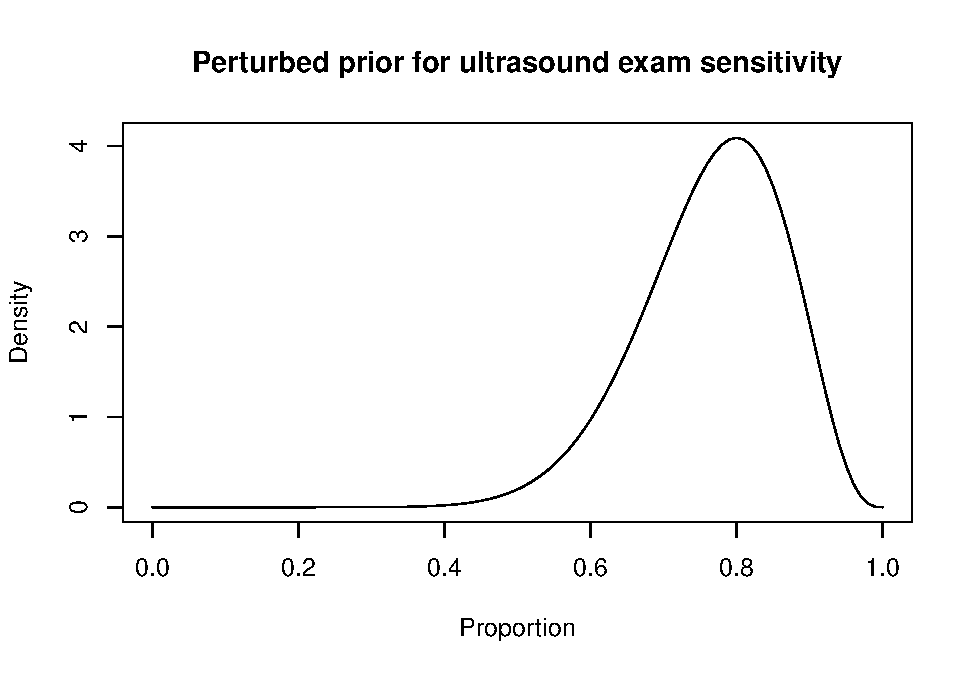
\includegraphics[keepaspectratio]{_main_files/_main_files/figure-latex/unnamed-chunk-96-1.pdf}}

\pandocbounded{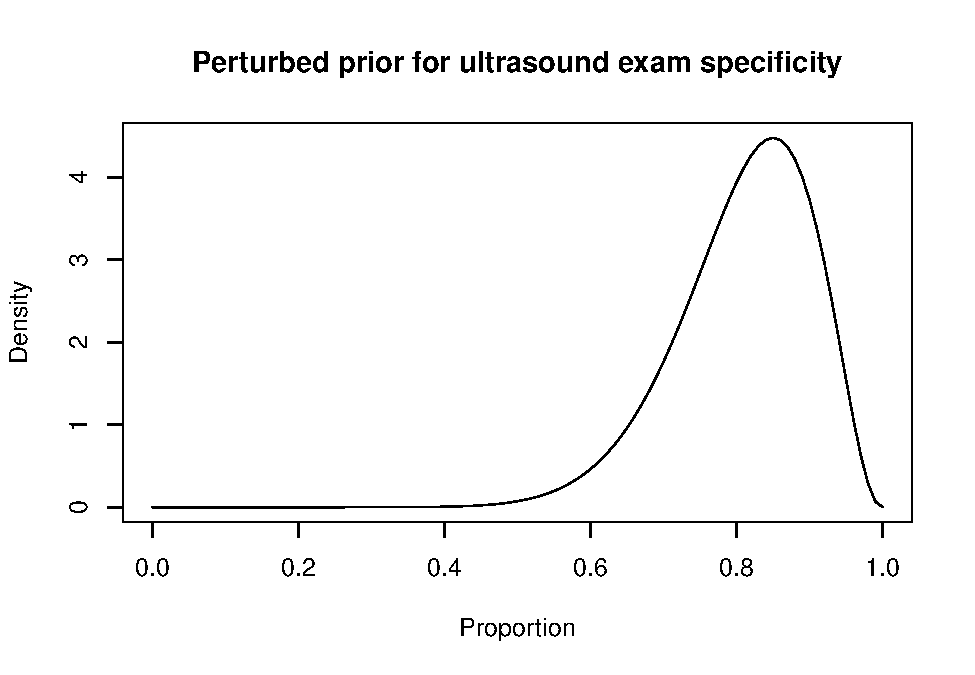
\includegraphics[keepaspectratio]{_main_files/_main_files/figure-latex/unnamed-chunk-97-1.pdf}}

Then, the results from the LCM with the informative and perturbed priors could be compared.

For instance, in exercise 3 we compared two conditionally independent diagnostic tests (PAG and US) in three populations (herd \#1, herd \#2, and herd \#3). For that model, though the model is identifiable, we could use the \href{https://www.sciencedirect.com/science/article/pii/S0093691X06001543?via\%3Dihub}{Romano et al.~(2006)} informative priors on US' Se and Sp. Then, we could run the same LCM, but with the perturbed US' Se and Sp priors suggested above. If we do that, we would obtain the following results:

\textbf{Table.} Results from a 2 tests, 3 populations LCM using different priors (literature-based \emph{vs.} perturbed informative priors on US' Se and Sp). The priors differing between LCM are indicated in bold.

\begin{longtable}[]{@{}
  >{\centering\arraybackslash}p{(\linewidth - 10\tabcolsep) * \real{0.1304}}
  >{\centering\arraybackslash}p{(\linewidth - 10\tabcolsep) * \real{0.2696}}
  >{\centering\arraybackslash}p{(\linewidth - 10\tabcolsep) * \real{0.1913}}
  >{\centering\arraybackslash}p{(\linewidth - 10\tabcolsep) * \real{0.0261}}
  >{\centering\arraybackslash}p{(\linewidth - 10\tabcolsep) * \real{0.1913}}
  >{\centering\arraybackslash}p{(\linewidth - 10\tabcolsep) * \real{0.1913}}@{}}
\toprule\noalign{}
\begin{minipage}[b]{\linewidth}\centering
\textbf{Parameter}
\end{minipage} & \begin{minipage}[b]{\linewidth}\centering
\textbf{Romano et al.~2006 priors}
\end{minipage} & \begin{minipage}[b]{\linewidth}\centering
\end{minipage} & \begin{minipage}[b]{\linewidth}\centering
\end{minipage} & \begin{minipage}[b]{\linewidth}\centering
\textbf{Perturbed priors}
\end{minipage} & \begin{minipage}[b]{\linewidth}\centering
\end{minipage} \\
\midrule\noalign{}
\endhead
\bottomrule\noalign{}
\endlastfoot
& \textbf{Prior} & \textbf{Posterior} & & \textbf{Prior} & \textbf{Posterior} \\
\textbf{Prev1} & Beta(1.0, 1.0) & 0.558 (0.496, 0.618) & & Beta (1.0, 1.0) & 0.556 (0.494, 0.617) \\
\textbf{Prev2} & Beta(1.0, 1.0) & 0.523 (0.440, 0.604) & & Beta (1.0, 1.0) & 0.520 (0.435, 0.603) \\
\textbf{Prev3} & Beta(1.0, 1.0) & 0.559 (0.452, 0.662) & & Beta (1.0, 1.0) & 0.557 (0.449, 0.657) \\
\textbf{Se US} & \textbf{Beta (100, 12)} & 0.925 (0.893, 0.954) & & \textbf{Beta (13.6, 4.1)} & 0.931 (0.890, 0.970) \\
\textbf{Sp US} & \textbf{Beta (100, 6.2)} & 0.977 (0.956, 0.990) & & \textbf{Beta (14.0, 3.3)} & 0.981 (0.957, 0.994) \\
\textbf{Se PAG} & Beta (1.0, 1.0) & 0.996 (0.981, 1.00) & & Beta (1.0, 1.0) & 0.996 (0.980, 1.00) \\
\textbf{Sp PAG} & Beta (1.0, 1.0) & 0.981 (0.934, 0.999) & & Beta (1.0, 1.0) & 0.977 (0.922, 0.999) \\
\end{longtable}

In this specific example, we can see that the results are virtually unchanged. Thus, we could say that our initial analysis was quite robust to the choice of prior distributions. Personally, we would present the LCM with the \href{https://www.sciencedirect.com/science/article/pii/S0093691X06001543?via\%3Dihub}{Romano et al.~(2006)} priors as our ``main'' model. If we do have valid information from the literature about one or many of the unknown parameters, then why not using them?

\chapter{Sample size}\label{sample-size}

When designing a study for estimating disease prevalence or diagnostic test accuracy we will want to evaluate the required sample size to achieve a certain precision in our test accuracy and disease prevalence estimates. In the following sections, we will first present, as a reminder, the method that can be used to estimate the sample size needed when a gold standard test is used for comparison. This method, however, is not appropriate when the test used for comparison is not a gold standard.

Then we will present a method specific for BLCM, which will provide a more accurate sample size estimation when imperfect tests are compared. This latter method will also be very helpful to quantify the impacts of choosing a given comparison test over another, or for choosing the prevalence that we should aim for in a second population of individuals.

\section{Method when comparing to a gold standard}\label{method-when-comparing-to-a-gold-standard}

Remember, the main parameters we want to estimate are a disease prevalence and a sensitivity and specificity, and these are all proportions. More precisely:

\begin{itemize}
\item
  The prevalence is \(\frac{\text{Number of diseased}}{\text{Number individuals}}\)
\item
  The sensitivity is \(\frac{\text{Number of test+}}{\text{Number diseased}}\)
\item
  The specificity is \(\frac{\text{Number of test-}}{\text{Number healthy}}\)
\end{itemize}

For any of these fractions, increasing the denominator will result in a decrease in the width of the 95\% confidence interval (i.e., a greater precision). To determine the denominator (i.e., the sample size) that could generate a given width for the 95\%CI, we could use the following, very simple Frequentist methods.

\(n=p*(1-p)*(\frac{1.96}{E})^{2}\)

Where \emph{n} is the required denominator, \emph{p} is the expected proportion, \emph{E} is the width of the 95\%CI we would like to achieve (i.e., the precision), and 1.96 is the \emph{Z} value corresponding to a type-I error rate of 0.05.

Alternatively, we could compute the width of the 95\%CI as function of a given denominator.

\(E=1.96*\sqrt{\frac{p*(1-p)}{n}}\)

Therefore, in order to estimate the required sample size, we would first need to provide an educated guess regarding:\\
- The true prevalence of disease we will observe;\\
- The sensitivity and specificity of the test under investigation.

As an example, if we were to design a study:\\
- On a population where we think the disease prevalence will be around 30\%;\\
- Using a test that we think will have a sensitivity of 85\% and specificity of 95\%;\\
- Where we would like to have a width of the 95\%CI of 10 percentage-points (i.e., +/- 5\% on each side of the median estimate).

We could use the following scripts to get an estimate of the required sample size.

\begin{Shaded}
\begin{Highlighting}[]
\CommentTok{\#Sample size for the prevalence}
\NormalTok{p }\OtherTok{\textless{}{-}} \FloatTok{0.30}
\NormalTok{E }\OtherTok{\textless{}{-}} \FloatTok{0.10}

\NormalTok{n }\OtherTok{\textless{}{-}}\NormalTok{ p}\SpecialCharTok{*}\NormalTok{(}\DecValTok{1}\SpecialCharTok{{-}}\NormalTok{p)}\SpecialCharTok{*}\NormalTok{(}\FloatTok{1.96}\SpecialCharTok{/}\NormalTok{E)}\SpecialCharTok{\^{}}\DecValTok{2}
\NormalTok{n}
\end{Highlighting}
\end{Shaded}

\begin{verbatim}
## [1] 80.6736
\end{verbatim}

For the prevalence, we would need 81 individuals to obtain a 95\%CI width of 10 percentage-points if the prevalence is around 30\%.

Note that, to obtain a 95\%CI width of 5 percentage-points:

\begin{Shaded}
\begin{Highlighting}[]
\CommentTok{\#Sample size for the prevalence}
\NormalTok{p }\OtherTok{\textless{}{-}} \FloatTok{0.30}
\NormalTok{E }\OtherTok{\textless{}{-}} \FloatTok{0.05}

\NormalTok{n }\OtherTok{\textless{}{-}}\NormalTok{ p}\SpecialCharTok{*}\NormalTok{(}\DecValTok{1}\SpecialCharTok{{-}}\NormalTok{p)}\SpecialCharTok{*}\NormalTok{(}\FloatTok{1.96}\SpecialCharTok{/}\NormalTok{E)}\SpecialCharTok{\^{}}\DecValTok{2}
\NormalTok{n}
\end{Highlighting}
\end{Shaded}

\begin{verbatim}
## [1] 322.6944
\end{verbatim}

We would now need 323 individuals.

Regarding the sensitivity, remember that the denominator will be the truly diseased individuals, rather than all sampled individuals.

\begin{Shaded}
\begin{Highlighting}[]
\CommentTok{\#Sample size for the sensitivity}
\NormalTok{p }\OtherTok{\textless{}{-}} \FloatTok{0.85}
\NormalTok{E }\OtherTok{\textless{}{-}} \FloatTok{0.10}

\NormalTok{n }\OtherTok{\textless{}{-}}\NormalTok{ p}\SpecialCharTok{*}\NormalTok{(}\DecValTok{1}\SpecialCharTok{{-}}\NormalTok{p)}\SpecialCharTok{*}\NormalTok{(}\FloatTok{1.96}\SpecialCharTok{/}\NormalTok{E)}\SpecialCharTok{\^{}}\DecValTok{2}
\NormalTok{n}
\end{Highlighting}
\end{Shaded}

\begin{verbatim}
## [1] 48.9804
\end{verbatim}

We would need 49 \textbf{diseased individuals} to obtain a 95\%CI width of 10 percentage-points if the sensitivity is around 85\%.

Regarding the specificity, again the denominator will be the truly healthy individuals, rather than all sampled individuals.

\begin{Shaded}
\begin{Highlighting}[]
\CommentTok{\#Sample size for the specificity}
\NormalTok{p }\OtherTok{\textless{}{-}} \FloatTok{0.95}
\NormalTok{E }\OtherTok{\textless{}{-}} \FloatTok{0.10}

\NormalTok{n }\OtherTok{\textless{}{-}}\NormalTok{ p}\SpecialCharTok{*}\NormalTok{(}\DecValTok{1}\SpecialCharTok{{-}}\NormalTok{p)}\SpecialCharTok{*}\NormalTok{(}\FloatTok{1.96}\SpecialCharTok{/}\NormalTok{E)}\SpecialCharTok{\^{}}\DecValTok{2}
\NormalTok{n}
\end{Highlighting}
\end{Shaded}

\begin{verbatim}
## [1] 18.2476
\end{verbatim}

We would need 18 \textbf{healthy individuals} to obtain a 95\%CI width of 10 percentage-points if the specificity is around 95\%.

Now, we need to reunite these different estimates together. For instance, we saw that measuring 81 individuals was enough to get the precision we needed for the prevalence of disease. But, with 81 individuals and a prevalence of 30\%, we would, theoretically, have 24 diseased (30\% of 81) and 57 healthy (70\% of 81) individuals. And we just computed that we needed 49 diseased individuals to get a precise estimate of the test's sensitivity.

In this case, we can see that the sensitivity is the limiting parameter. We could, thus, possibly recruit \textbf{a minimum} of 150 individuals and, hopefully, 50 will be diseased and 100 will be healthy. With that latter sample, we would possibly achieve the precision needed for the test's sensitivity, and we would exceed what we needed for the test's specificity and for disease prevalence. Of course this will work if our guess estimates were not too ``off the mark''.

\textbf{This basic method, however, is not considering the loss of power that will occur when comparing imperfect tests with one another (as compared to comparing a novel test to a gold-standard test). This should, therefore, be considered as an overoptimistic scenario if the test used for comparison is not a gold standard.}

\section{Method for the Hui-Walter BLCM}\label{method-for-the-hui-walter-blcm}

\href{https://www.sciencedirect.com/science/article/pii/S0167587705001674?via\%3Dihub}{Georgiadis et al.~(2005)} proposed a method to calculate sample size to estimate disease prevalence, sensitivity and specificity with a desired precision, when using the \href{https://www.jstor.org/stable/2530508?seq=1}{Hui and Walter (1980)} model (two conditionally independent tests for screening individuals from two populations). In their article, \href{https://www.sciencedirect.com/science/article/pii/S0167587705001674?via\%3Dihub}{Georgiadis et al.~(2005)} provided the hyperlink to an Excel spreadsheet template. We included this spreadsheet in the course material.

Briefly, we need to provide our best guess on:\\
- Disease prevalence in population 1 (\(\pi1\));\\
- Disease prevalence in population 2 (\(\pi2\));\\
- Sensitivity of the first (\(Se1\)) and second test (\(Se2\));\\
- Specificity of the first (\(Sp1\)) and second test (\(Sp2\)).

And, then, the desired 95\% BCI width for these different parameters.

Below is a screen capture of the spreadsheet. In this case, we proposed to study two populations where:\\
- Disease prevalence (\(\pi1\) and \(\pi2\)) would be 0.10 and 0.70;\\
- Sensitivity of the two tests (\(Se1\) and \(Se2\)) would be 0.85 and 0.95;\\
- Specificity of the two tests (\(Sp1\) and \(Sp2\)) would both be 0.95;\\
- Desired width of the 95\% BCI for disease prevalence (\(\pi1\) and \(\pi2\)) would be 0.15;\\
- Desired width of the 95\% BCI for sensitivity (\(Se1\) and \(Se2\)) would be 0.20;\\
- Desired width of the 95\% BCI for specificity (\(Sp1\) and \(Sp2\)) would be 0.10;

\begin{figure}
\centering
\pandocbounded{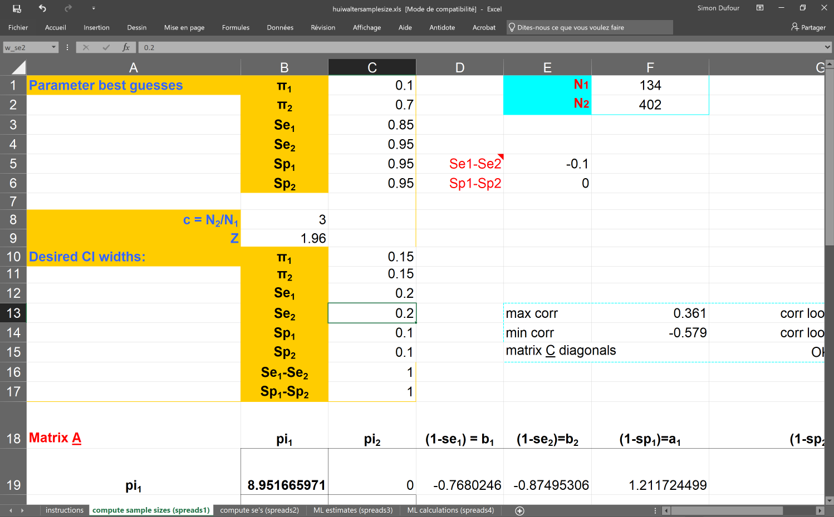
\includegraphics[keepaspectratio]{_main_files/Figures/Georgiadis spreadsheet.png}}
\caption{\textbf{Excel spreadsheet used to estimate sample size for BLCM comparing two independent tests in two populations.}}
\end{figure}

\strut \\
Additional information are provided in the spreadsheet, but we can already see that we would need to sample 134 individuals from the low (10\%) prevalence population (\emph{N1}) and 402 from the high (70\%) prevalence population (\emph{N2}) to obtain the desired width for the 95\% BCIs.

Again, this will work if our guess estimates were not too ``off the mark''. One additional note, when using the \href{https://www.sciencedirect.com/science/article/pii/S0167587705001674?via\%3Dihub}{Georgiadis et al.~(2005)} method, we are not considering any informative priors that we may want to use. Typically, if we were to use informative priors on some or all of the unknown parameters the width of the 95\% BCI will possibly be modified. For instance, if we provided relatively narrow priors for a given parameter, and if these priors agree closely with the observed data, then the 95\% BCI could be more precise than anticipated (i.e., narrower). On the other hand, narrow priors which are not consistent with the observed data would possibly yield larger 95\% BCI.

Nevertheless, this spreadsheet is quite handy to get rough sample size estimates. It is also quite useful to explore, for instance, how larger differences in disease prevalence between populations can improve the study power. It is also very interesting to investigate how the choice of the second test used for comparison will affect the study power.

As an example, in the following figure we illustrated, for the \href{https://www.jstor.org/stable/2530508?seq=1}{Hui and Walter (1980)} model, how the \textbf{difference in prevalence between the two populations} would impact sample size. As you can see, for this specific scenario, targeting populations with more important prevalence differences could have a tremendous impact on power of the study. For instance, in this example, \textbf{with prevalence of 0.10 and 0.20 in the first and second population, a total of 14356 individuals would have to be tested to achieve the desired precision. On the other hand, with prevalence of 0.10 and 0.70 in the first and second population, only 218 individuals would have to be tested.}

\begin{figure}
\centering
\pandocbounded{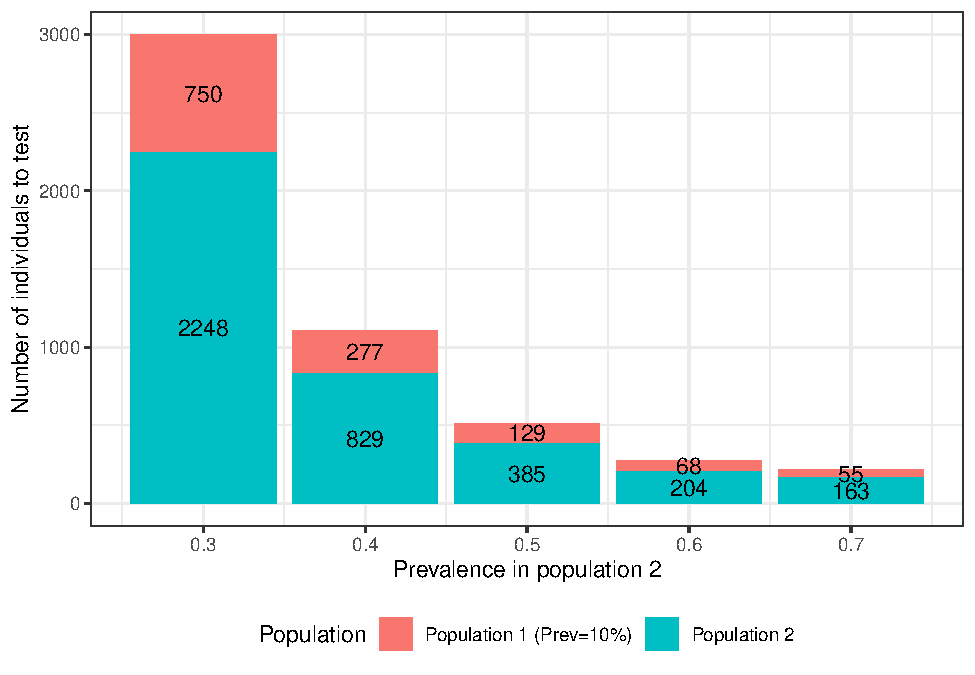
\includegraphics[keepaspectratio]{_main_files/_main_files/figure-latex/unnamed-chunk-106-1.pdf}}
\caption{\label{fig:unnamed-chunk-106}Number of individuals to test as function of the difference in prevalence between populations. For these calculations we assumed that: 1) the first population has a prevalence of disease of 0.10; 2) the two tests are expected to have Se and Sp of 0.90; 3) we are only interested in estimating the accuracy of the first test; and 4) we wish to obtain a 95 BCI width of \textless20 percentage-points (i.e., \textless{} +/- 10 percentage points) when reporting accuracy of the first test.}
\end{figure}

Now, we could use two populations with expected disease prevalence of 0.10 and 0.50, but we are, this time, wondering what would be the best test to use for comparison so we can achieve the required precision with the smallest possible sample size. Below, we quantified how a change in the specificity of the second test would affect the require sample size. We see that, \textbf{if the test used for comparison has a specificity of 0.70, we will need to test 1664 individuals to achieve the desired precision. On the other hand, if this test specificity is 1.0 (i.e., no false positive results), only 218 individuals would have to be tested.}

\begin{figure}
\centering
\pandocbounded{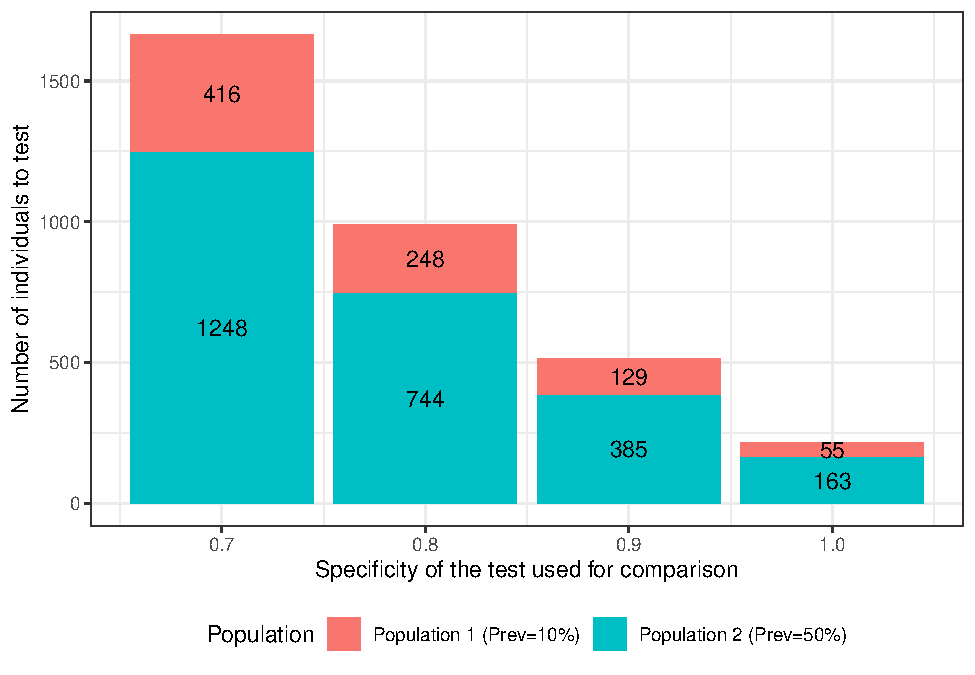
\includegraphics[keepaspectratio]{_main_files/_main_files/figure-latex/unnamed-chunk-107-1.pdf}}
\caption{\label{fig:unnamed-chunk-107}Number of individuals to test as function of specificity of the test used for comparison. For these calculations we assumed that: 1) the first and second population have disease prevalence of 0.10 and 0.50; 2) the test under investigation is expected to have a Se and Sp of 0.90; 3) we are only interested in estimating the accuracy of this first test; 4) we wish to obtain a 95 BCI width of \textless20 percentage-points (i.e., \textless{} +/- 10 percentage points) when reporting accuracy of the first test; and 5) the test used for comparison is expected to have a sensitivity of 0.90.}
\end{figure}

We could also quantify how a change in the sensitivity of the test used for comparison would affect the require sample size. We see that, \textbf{if the test has a sensitivity of 0.70, we will need to test 851 individuals to achieve the desired precision. On the other hand, if the test's sensitivity is 1.0 (i.e., no false negative results), only 420 individuals would have to be tested.}

\begin{figure}
\centering
\pandocbounded{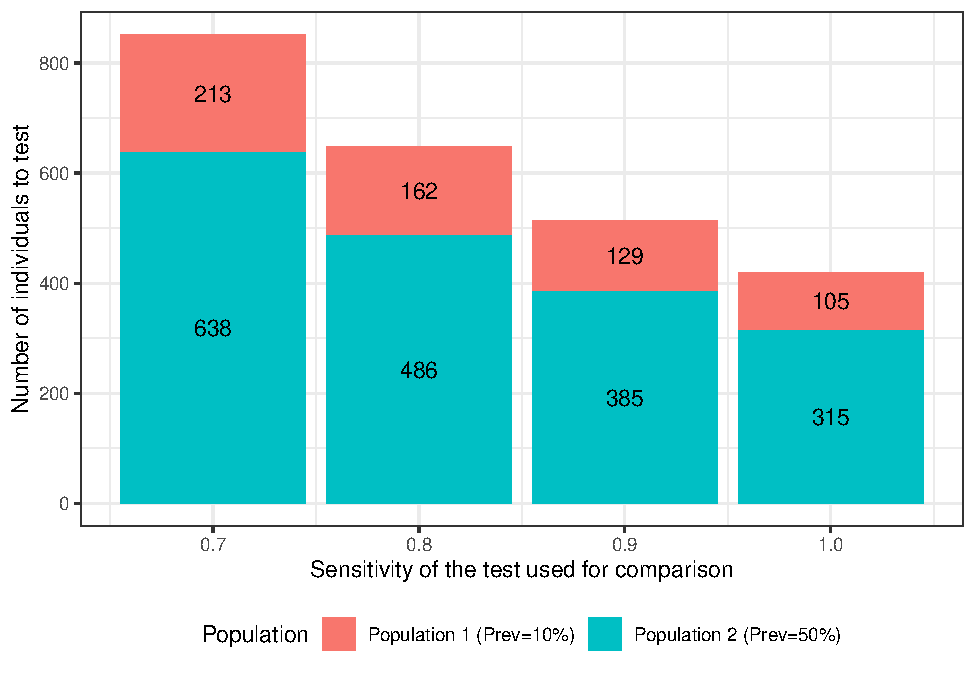
\includegraphics[keepaspectratio]{_main_files/_main_files/figure-latex/unnamed-chunk-108-1.pdf}}
\caption{\label{fig:unnamed-chunk-108}Number of individuals to test as function of sensitivity of the test used for comparison. For these calculations we assumed that: 1) the first and second population have disease prevalence of 0.10 and 0.50; 2) the test under investigation is expected to have a Se and Sp of 0.90; 3) we are only interested in estimating the accuracy of this first test; 4) we wish to obtain a 95 BCI width of \textless20 percentage-points (i.e., \textless{} +/- 10 percentage points) when reporting accuracy of the first test; and 5) the test used for comparison is expected to have a specificity of 0.90.}
\end{figure}

For this specific scenario, we can see that there is a greater gain in study power, when improving the specificity of the test used for comparison \emph{vs.} improving its sensitivity. Indeed, with prevalence of 0.10 and 0.50 in the two populations, we have more healthy individuals than diseased individuals. As a consequence, in this example, an increase in the specificity of one of the tests was a better strategy to reduce misclassification issues than increasing its sensitivity. Finding a second test with the latter properties is often doable. For instance, for many diseases we have tests that can lead to the isolation of the microorganism and, if the microorganism is a strict pathogen, then such a test would be deemed to be 100\% specific. As a comparison, using the same example, if we would have used a gold standard test for comparison, 196 individuals would have to be tested, as compared to 218 when using a second test with perfect specificity and a sensitivity of 0.90. Not a huge difference\ldots{} And in many cases, another imperfect test would be cheaper than a gold standard test, and that is when a gold standard test is actually available (often it is not).

As we can see, conducting an \emph{a priori} sample size estimation is extremely important when designing a diagnostic test validation study, since relatively minor decisions regarding the study design can greatly affect its power. One final note, if we are planning a study with more than two populations, or more than two tests, this spreadsheet could still be used to obtain a ``worst-case scenario'' sample size estimation (i.e., study power would mainly be increased, not decreased, by adding extra populations or tests).

\chapter{Exercise 6 - Sample size estimation and study design}\label{exercise-6---sample-size-estimation-and-study-design}

\section{Questions}\label{questions-5}

For the following questions we will work with the Microsoft Excel sheet developed by \href{https://www.sciencedirect.com/science/article/pii/S0167587705001674?via\%3Dihub}{Georgiadis et al.~(2005)}. You will find this document in the folder named ``Exercise 6 - Sample size estimation and study design'' in the course materials.

\textbf{1.} Imagine that you are helping a research team for planning a study aiming at estimating the accuracy of a new test for detection of \emph{Staphylococcus aureus} intra-mammary infections (\textbf{IMI}) using milk samples from dairy cattle.

\begin{itemize}
\tightlist
\item
  The diagnostic test development team is expecting that this new test will have a \textbf{sensitivity (Se) around 95\%} and a \textbf{specificity (Sp) around 90\%}.\\
\item
  They would like to report accuracy of the new test with a \textbf{precision of +/- 5 percentage-points}, but they are not really interested in reporting the disease prevalence nor the second test's accuracy.\\
\item
  In the literature, \href{https://www.sciencedirect.com/science/article/pii/S0022030210006922?via\%3Dihub}{Dohoo et al.~(2011)} reported a \textbf{Se and Sp of, respectively, 90\% and 100\% for conventional bacteriological culture}.\\
\item
  Moreover, a veterinary practitioner working with the test's development team indicated that, when sampling a population of cows without specific selection criteria, we could expect a \emph{S. aureus} IMI \textbf{prevalence of 5\%}.\\
\item
  The practitioner also indicated that, \textbf{in a population of cows with persistently high somatic cells count (SCC), we would possibly have 20\% of \emph{S. aureus} IMI}.
\end{itemize}

How would you see the study design for this study and what would be the number of cows to test?

\textbf{2.} The diagnostic test development team was not too happy with the number of tests required by the darn epidemiologist (as usual). They told you that they have the budget for testing 400 cows and are asking what would be the precision in the accuracy parameters (Se and Sp) of the new test that they could achieve with such a sample size?

\textbf{3.} One of the person from the test's development team suggested to use for comparison, PCR instead of conventional bacteriological culture. Indeed, PCR as a Se of 99\% and Sp of 99\%, so quite superior to that of culture (90\% and 100\%). They are asking if, with 400 cows, they could now achieve a more precise estimation of the new test accuracy?

\textbf{4.} The research team is getting quite frustrated with your answers. The practitioner on the test's development team indicate that, when sampling cows that were positive to \emph{S. aureus} in the past, we could expect that 50\% of them would still be positive. They are asking if this could be a ``better'' second population in term of study power? When comparing the new test to bacteriological culture in a population of cows selected randomly and a population of cows that were positive to \emph{S. aureus} in the past, what would be the precision in the accuracy parameters (Se and Sp) of the new test that could be obtained using 400 cows?

\section{Answers}\label{answers-5}

\textbf{1.} How would you see the study design for this study and what would be the number of cows to test?

\textbf{Answer:} We could imagine a validation test study where the new test and conventional milk bacteriological culture will be applied to samples coming from a number of cows in two populations:\\
1- Randomly chosen cows (anticipated prevalence of 5\%)\\
2- Cows with persistently high SCC (anticipated prevalence of 20\%)

Using this approach we would estimate that 1330 cows would be needed; 333 cows from the low prevalence population and 997 from the high prevalence population. This is, of course, assuming that the tests are conditionally independent.

\textbf{2.} What would be the precision in the accuracy parameters (Se and Sp) of the new test when testing 400 cows?

\textbf{Answer:} In the Excel sheet, we had to play with the desired CI width for the Se and Sp of the first test until we reached a total sample size of approximately 400 cows. Therefore, you may have obtained results that are slightly different than us. But, in our case, we were approaching 400 animals (exactly 411 animals, actually) when using CI width of 0.18 for Se and of 0.16 for Sp, thus \textbf{+/- 9 and +/- 8 percentage-points around the median Se and Sp estimates, respectively}.

\textbf{3.} What would be the precision of the new test accuracy when using PCR as comparison and with 400 cows?

\textbf{Answer:} If we use 99\% for the second test's Se and Sp and play with the first test's Se and Sp desired CI width until we get around 400 cows to test, we find that, with 400 cows (403 to be precise), \textbf{we would report Se and Sp with precision of +/- 14 and +/- 8 percentage-points around the median estimates, respectively.} It's worst than before! As you can see, when disease prevalence is low, having a second test with a perfect Sp (i.e., bacteriological milk culture in this case) can have a tremendous impact!

\textbf{4.} What would be the precision of the new test accuracy when using a population of cow selected randomly and a population of cows that were positive to \emph{S. aureus} in the past, and with a total of 400 cows tested?

\textbf{Answer:} With these parameters we would report Se and Sp with precision of \textbf{+/- 5 and +/- 7 percentage-points around the median estimates, respectively.} The test's development team is super happy with this; they now love epidemiologists. When you leave the room you hear them say:

\pandocbounded{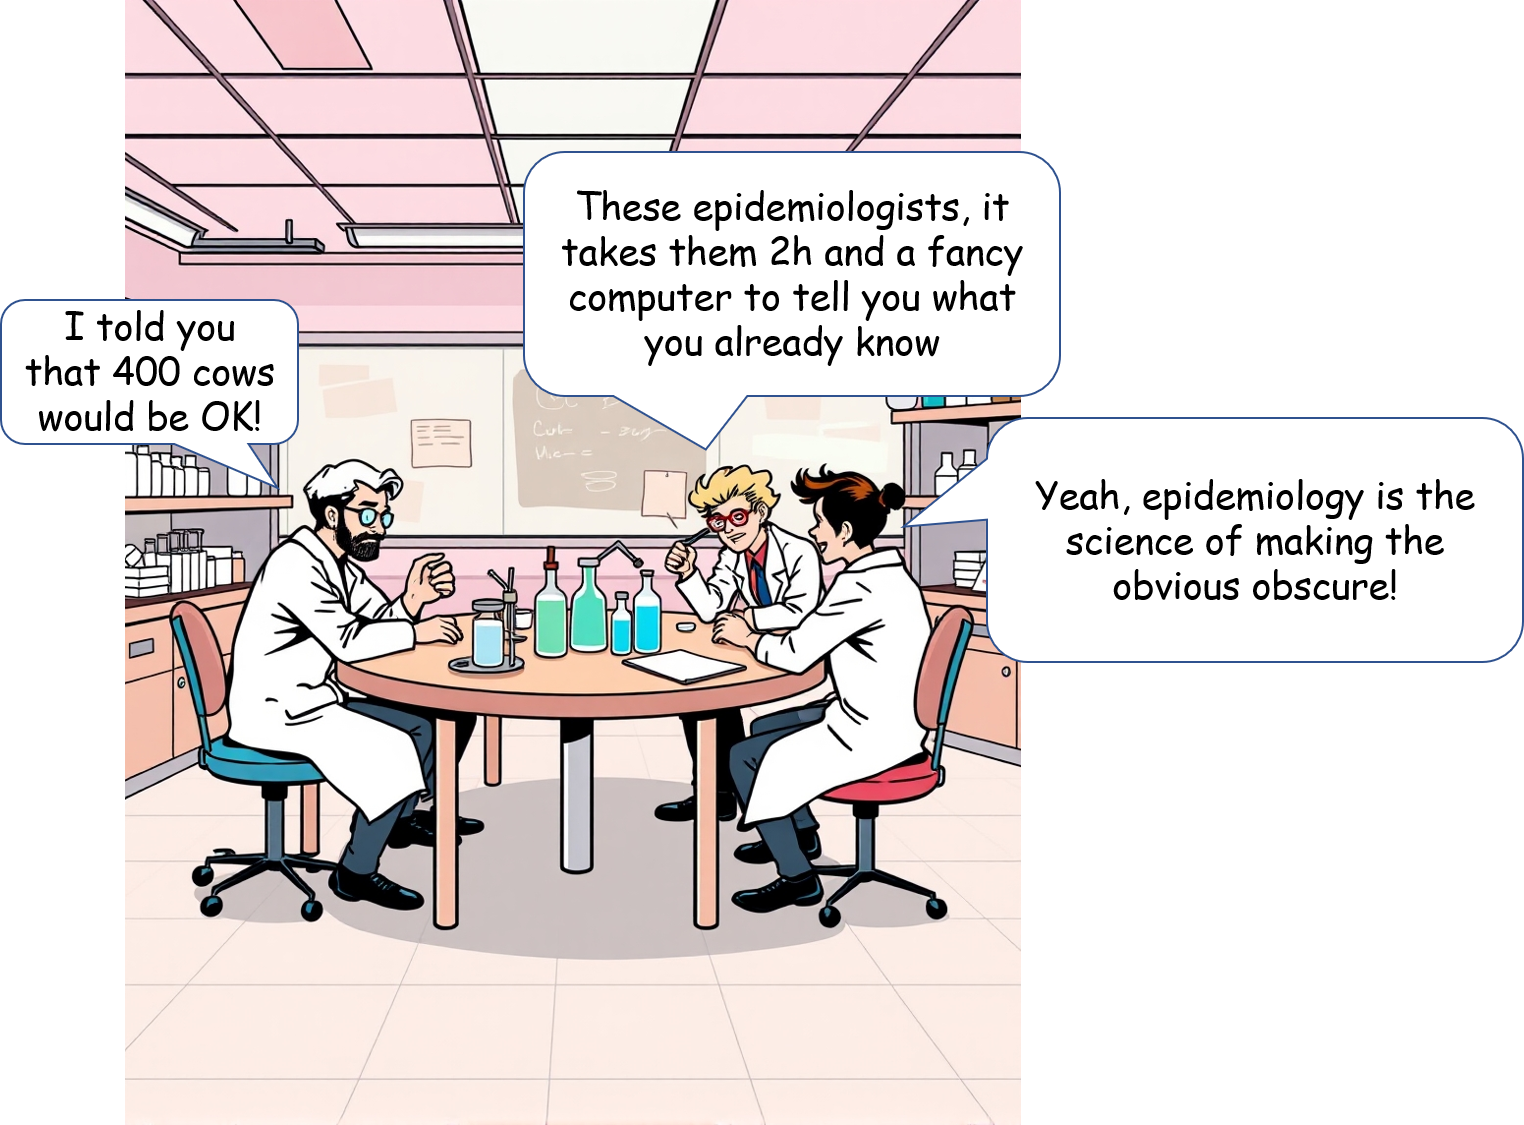
\includegraphics[keepaspectratio]{_main_files/Figures/scientists.png}}

\bibliography{book.bib,packages.bib}

\end{document}
